\chapter{fearful symmetries} 
\label{sec:symmetries}
\rhead[]{\leftmark}
\lstset{style=6502Style}
\lstset{ 
   aboveskip=5pt,
   belowskip=0pt,
}

% \newdate{..label..}{..date..}{..info..}
\newcommand\addItem[2]%
{
  \expandafter\def\csname row:#1\endcsname{#2}%
}

% \showItem{..label..}
\newcommand\showItem[1]%
{\expandafter\csname row:#1\endcsname}


% \getItem{..label..}
\newcommand\getItem[1]%
{\noindent
  \text{\showItem{#1}}
  \par
}
% An array of captions 
\addItem{0}{Star One: Y-Axis, X-Y Symmetry, X-Axis Symmetry, Quad Symmetry}
\addItem{1}{The Twist: Y-Axis, X-Y Symmetry, X-Axis Symmetry, Quad Symmetry}
\addItem{2}{La Llamita}
\addItem{3}{Star Two}
\addItem{4}{Deltoid}
\addItem{5}{Diffused}
\addItem{6}{Multi-Cross}
\addItem{7}{Pulsar}
\addItem{8}{Custom Pattern 1}
\addItem{9}{Custom Pattern 2}
\addItem{10}{Custom Pattern 3}
\addItem{11}{Custom Pattern 4}
\addItem{12}{Custom Pattern 5}
\addItem{13}{Custom Pattern 6}
\addItem{14}{Custom Pattern 7}

\begin{definition}[Jeffrey Says\index{Jeffrey Says}]
\setlength{\intextsep}{0pt}%
\setlength{\columnsep}{3pt}%
\begin{wrapfigure}{l}{0.12\textwidth}

\includegraphics[width=\linewidth]{src/callout/psych.png} 
\end{wrapfigure}
\small
\textbf{Press S to change the Symmetry.} \\
  The pattern gets reflected in various planes, or not at all according to the setting.
\\
\\
\end{definition}

There are 4 possible symmetries for displaying patterns in Psychedelia. As we saw when
reviewing the code for the magazine listing the painting of the symmetries is managed
by \icode{PaintPixelForCurrentSymmetry\index{PaintPixelForCurrentSymmetry}}. There it was hardcoded to use a simple
reflection symmetry along the X-axis, but the commercial version of Psychedelia has to
go a little further and support along all three possible axes. 

Now that the player can change the active symmetry at any time, there is also a little more
book-keeping for Psychedelia to do in terms of recognizing the active symmetry for each
step in the pattern's evolution. In this chapter we'll take a look at how this 
\textit{fascinating} bit of accounting works and console ourselves the while with some
pretty pictures of the symmetry rendering in operation. First, a couple of pretty pictures.
Then some potentially tedious unpacking of code.

\foreach \l in {0,...,1}
{
  \begin{figure}[H]
      \centering
        \vspace*{-6cm}
        \hspace*{-8cm}
        \includegraphics[width=20cm]{src/symmetries/pattern\l_1-45.png}%
        \hspace*{-12cm}
        \includegraphics[width=20cm]{src/symmetries/pattern\l_2-45.png}\\
        \vspace*{-13cm}
        \hspace*{-7cm}
        \includegraphics[width=20cm]{src/symmetries/pattern\l_3-45.png} \\
        \vspace*{-20cm}
        \includegraphics[width=20cm]{src/symmetries/pattern\l_4-45.png}
        \vspace*{-4cm}
  \caption*{\getItem{\l}}
  \end{figure}

}%

\clearpage
\textbf{Lines 1210-1231. \icode{\textbf{CheckKeyboardInput\index{CheckKeyboardInput}}}}
\begin{lstlisting}[escapechar=\%]
;-------------------------------------------------------
; CheckKeyboardInput%\index{CheckKeyboardInput}%
;-------------------------------------------------------
CheckKeyboardInput%\index{CheckKeyboardInput}%   
        ...
        LDA lastKeyPressed%\index{lastKeyPressed}%
        ...
MaybeSPressed   
        CMP #KEY_S ; 'S' pressed.
        BNE MaybeLPressed

        ; Check if shift was pressed too.
        LDA shiftPressed%\index{shiftPressed}%
        AND #$01
        BEQ JustSPressed%\index{JustSPressed}%

        LDA tapeSavingInProgress
        BNE JustSPressed%\index{JustSPressed}%
        ; Shift + S pressed: Save.
        JMP PromptToSave%\index{PromptToSave}%
        ; Returns

        ; 'S' pressed. 
JustSPressed%\index{JustSPressed}%   
        INC currentSymmetrySetting%\index{currentSymmetrySetting}%
        LDA currentSymmetrySetting%\index{currentSymmetrySetting}%
        CMP #$05
        BNE SetUpYRegisterToGetText
        LDA #$00
        STA currentSymmetrySetting%\index{currentSymmetrySetting}%

SetUpYRegisterToGetText   
        ASL 
        ASL 
        ASL 
        ASL 
        TAY 
        JSR ClearLastLineOfScreen%\index{ClearLastLineOfScreen}%

        ; currentSymmetrySetting%\index{currentSymmetrySetting}% is in Y
        LDX #$00
WriteSymmetryDescription   
        LDA txtSymmetrySettingDescriptions,Y
        STA lastLineBufferPtr,X
        INY 
        INX 
        CPX #$10
        BNE WriteSymmetryDescription

        JMP WriteLastLineBufferToScreen%\index{WriteLastLineBufferToScreen}%
        ;Returns
\end{lstlisting}
\clearpage

\rhead[]{\icode{CheckKeyboardInput\index{CheckKeyboardInput}}}
\textbf{Lines 1210-1231. \icode{\textbf{MaybeSPressed}}:} This is the routine that detects when the player has selected a new
symmetry by pressing the 'S' key. It is part of the much larger routine \icode{CheckKeyboardInput\index{CheckKeyboardInput}} which periodically checks
for keyboard input by polling the byte at address \icode{\$00C5} (which we label \icode{lastKeyPressed\index{lastKeyPressed}}). This address always
contains the value of the most recently pressed key on the keyboard.

If Shift was pressed the user is actually looking to trigger a save, in which case execution passes to \icode{PromptToSave\index{PromptToSave}}.

Otherwise we increment \icode{currentSymmetrySetting\index{currentSymmetrySetting}}, which is the variable we use for storing the currently selected symmetry.
Each press of the 'S' key increments the value of \icode{currentSymmetrySetting\index{currentSymmetrySetting}} until it reaches 5. Once that happens, we 
reset it to zero again (\icode{LDA \#\$00; STA currentSymmetrySetting\index{currentSymmetrySetting}}).

\textbf{Lines 1236-1254. \icode{\textbf{SetUpYRegisterToGetText}}:} What is the series of \icode{ASL} instructions doing? A tricky
piece of business of course. We have loaded \icode{currentSymmetrySetting\index{currentSymmetrySetting}} to the \icode{A} register (\icode{LDA currentSymmetrySetting\index{currentSymmetrySetting}}) and it has a value between 0 and 4.
\icode{ASL} performs a leftward bit-shift on the \icode{A} register. A single left-shift has an interesting property - it doubles the
value of the byte. A second left-shift will double it again, and so on. So our four {ASL} instructions have the effect of turning 1 into
16, 2 into 32, 3 into 48, and 4 into 64. This has the very useful effect of giving us an index into the description of each symmetry!

\begin{lstlisting}[escapechar=\%]
txtSymmetrySettingDescriptions 
        .TEXT 'NO SYMMETRY     ' ; Starts at index 0
        .TEXT 'Y-AXIS SYMMETRY ' ; Starts at index 16
        .TEXT 'X-Y SYMMETRY    ' ; Starts at index 32
        .TEXT 'X-AXIS SYMMETRY ' ; Starts at index 48
        .TEXT 'QUAD SYMMETRY   ' ; Starts at index 64
\end{lstlisting}

So when we take our resulting value and load it into the \icode{Y} register all our \icode{Write\-Symmetry\-Description} needs to do is start at the 
index given by \icode{Y} and write out the next 16 bytes to the screen, displaying the selected symmetry briefly to the player.


\clearpage
\rhead[]{\leftmark}
\hspace{-1cm}
\begin{minipage}[b]{0.50\linewidth}                                       
  \begin{figure}[H]
      \centering
        \vspace*{-1cm}
        \hspace*{-2cm}
        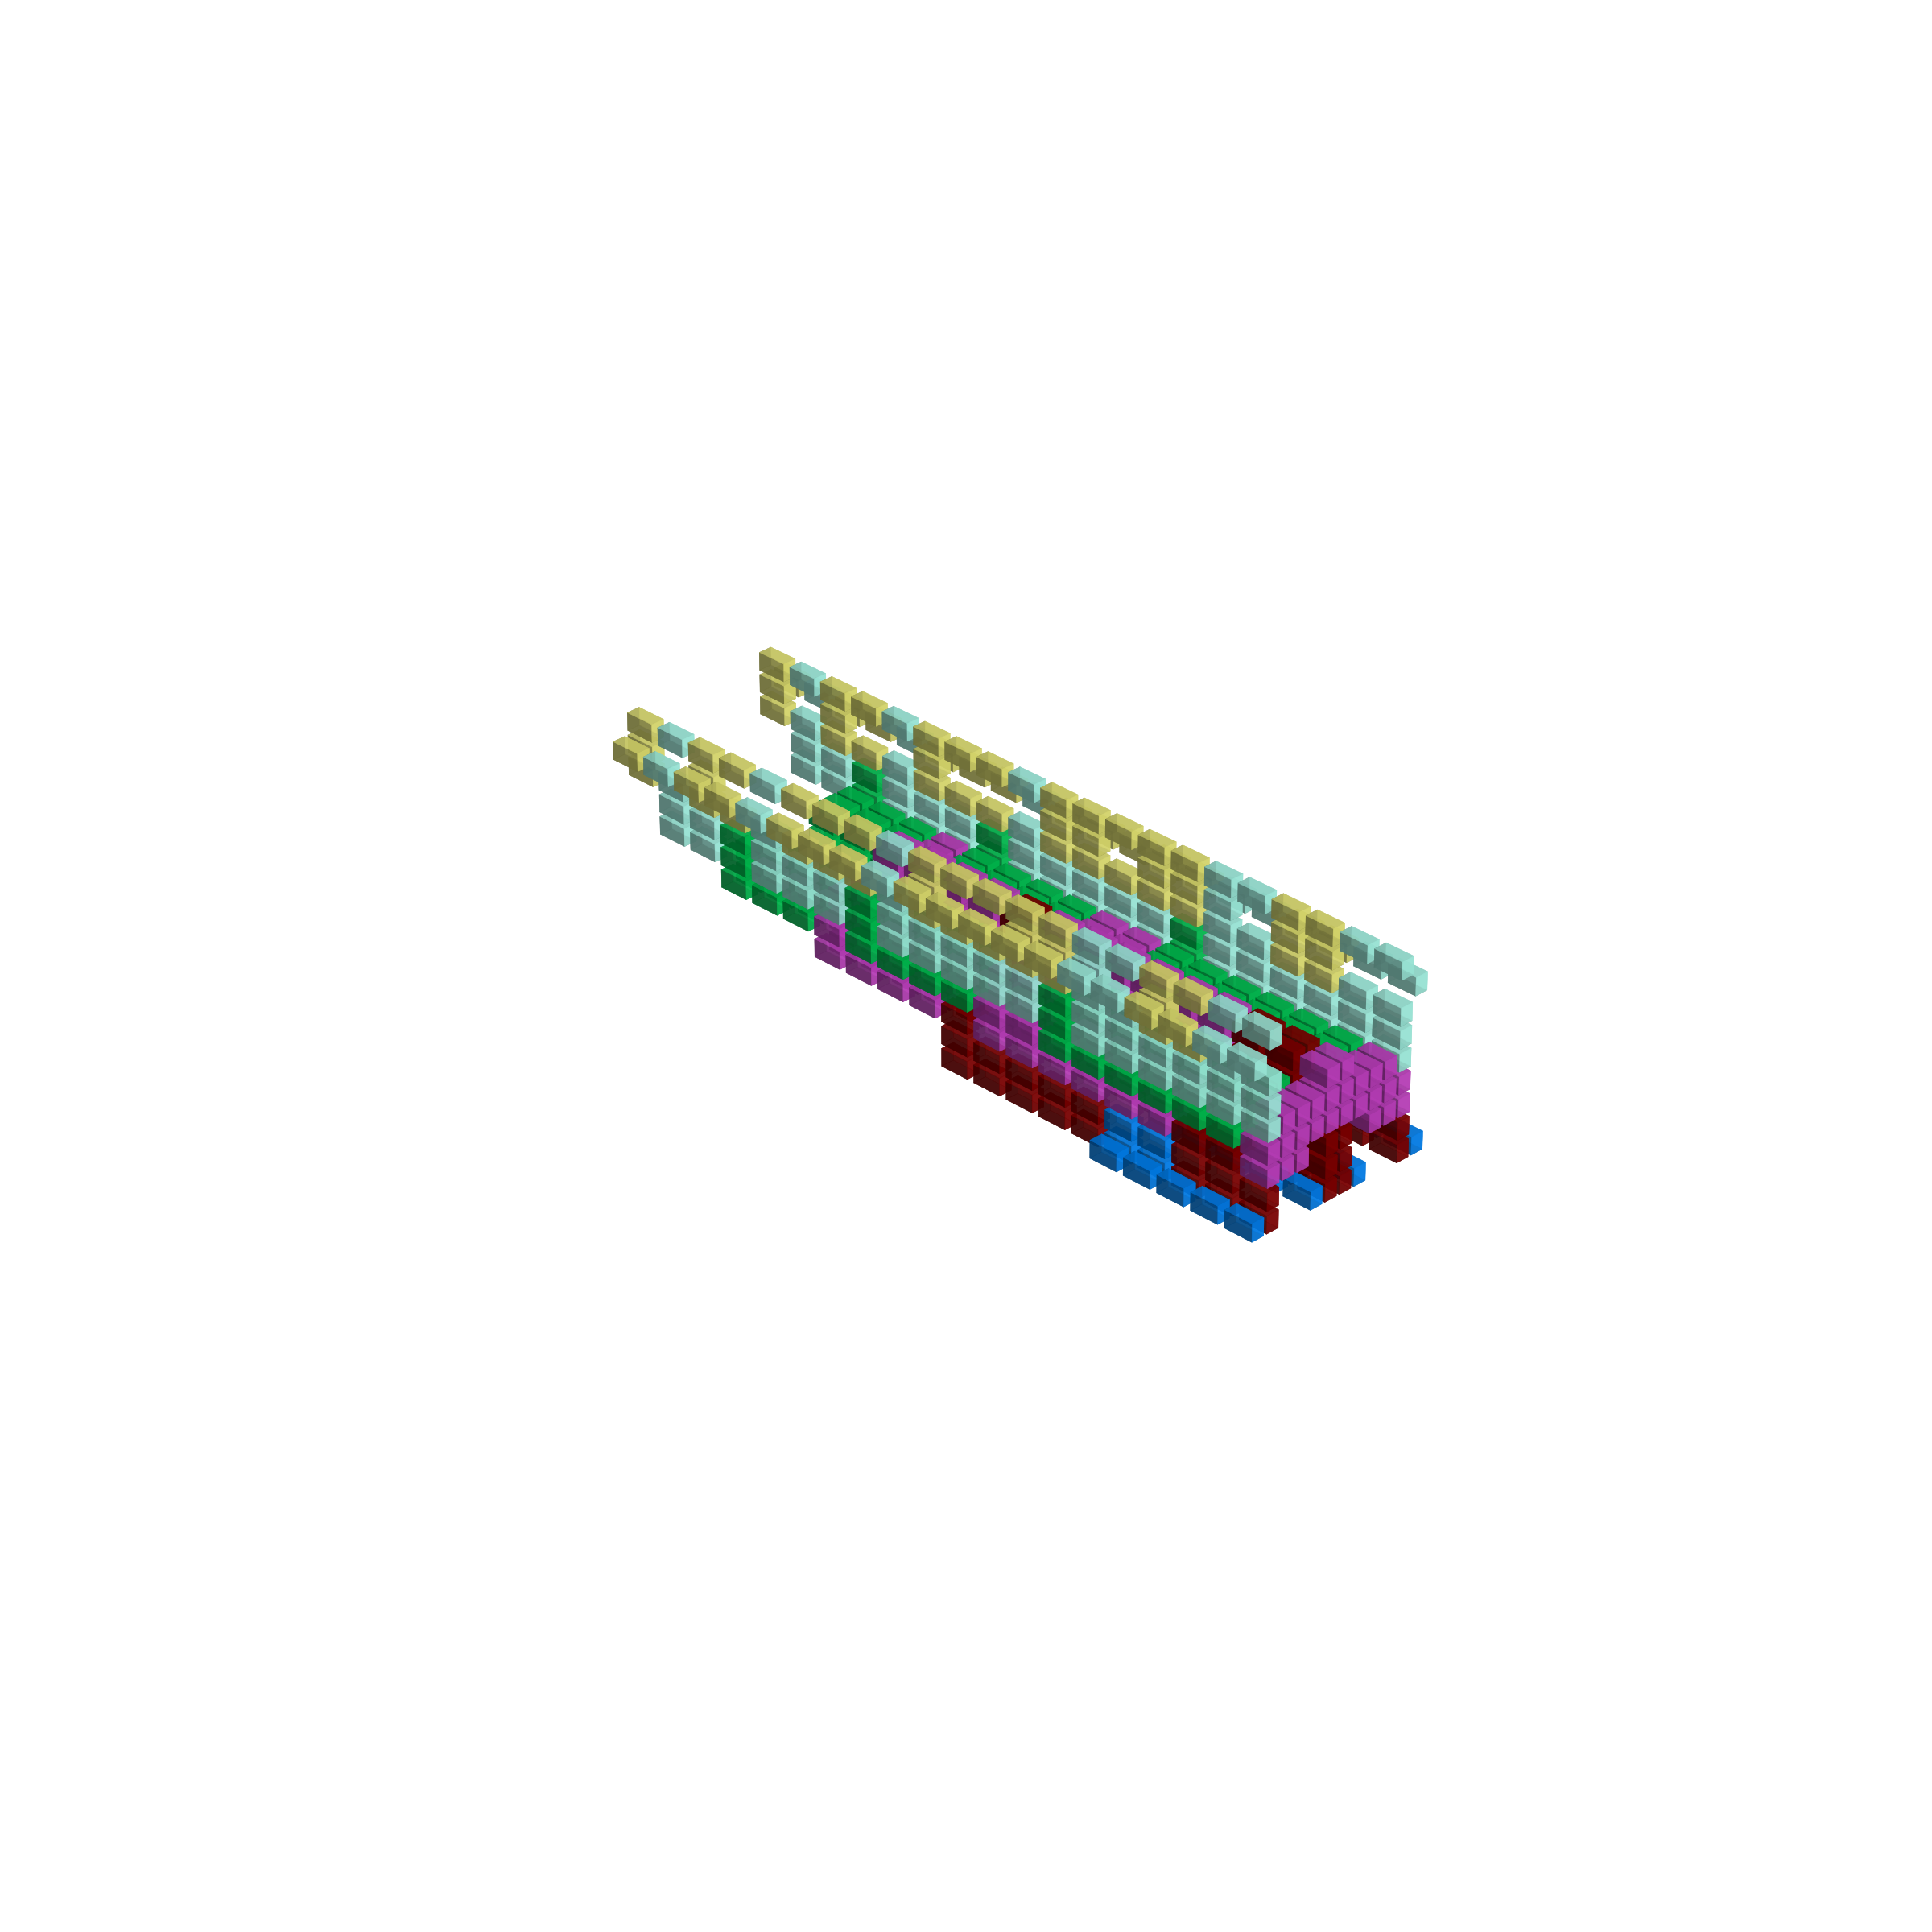
\includegraphics[width=8cm]{src/symmetries/pattern2_1-45.png}%
        \hspace*{-4cm}
        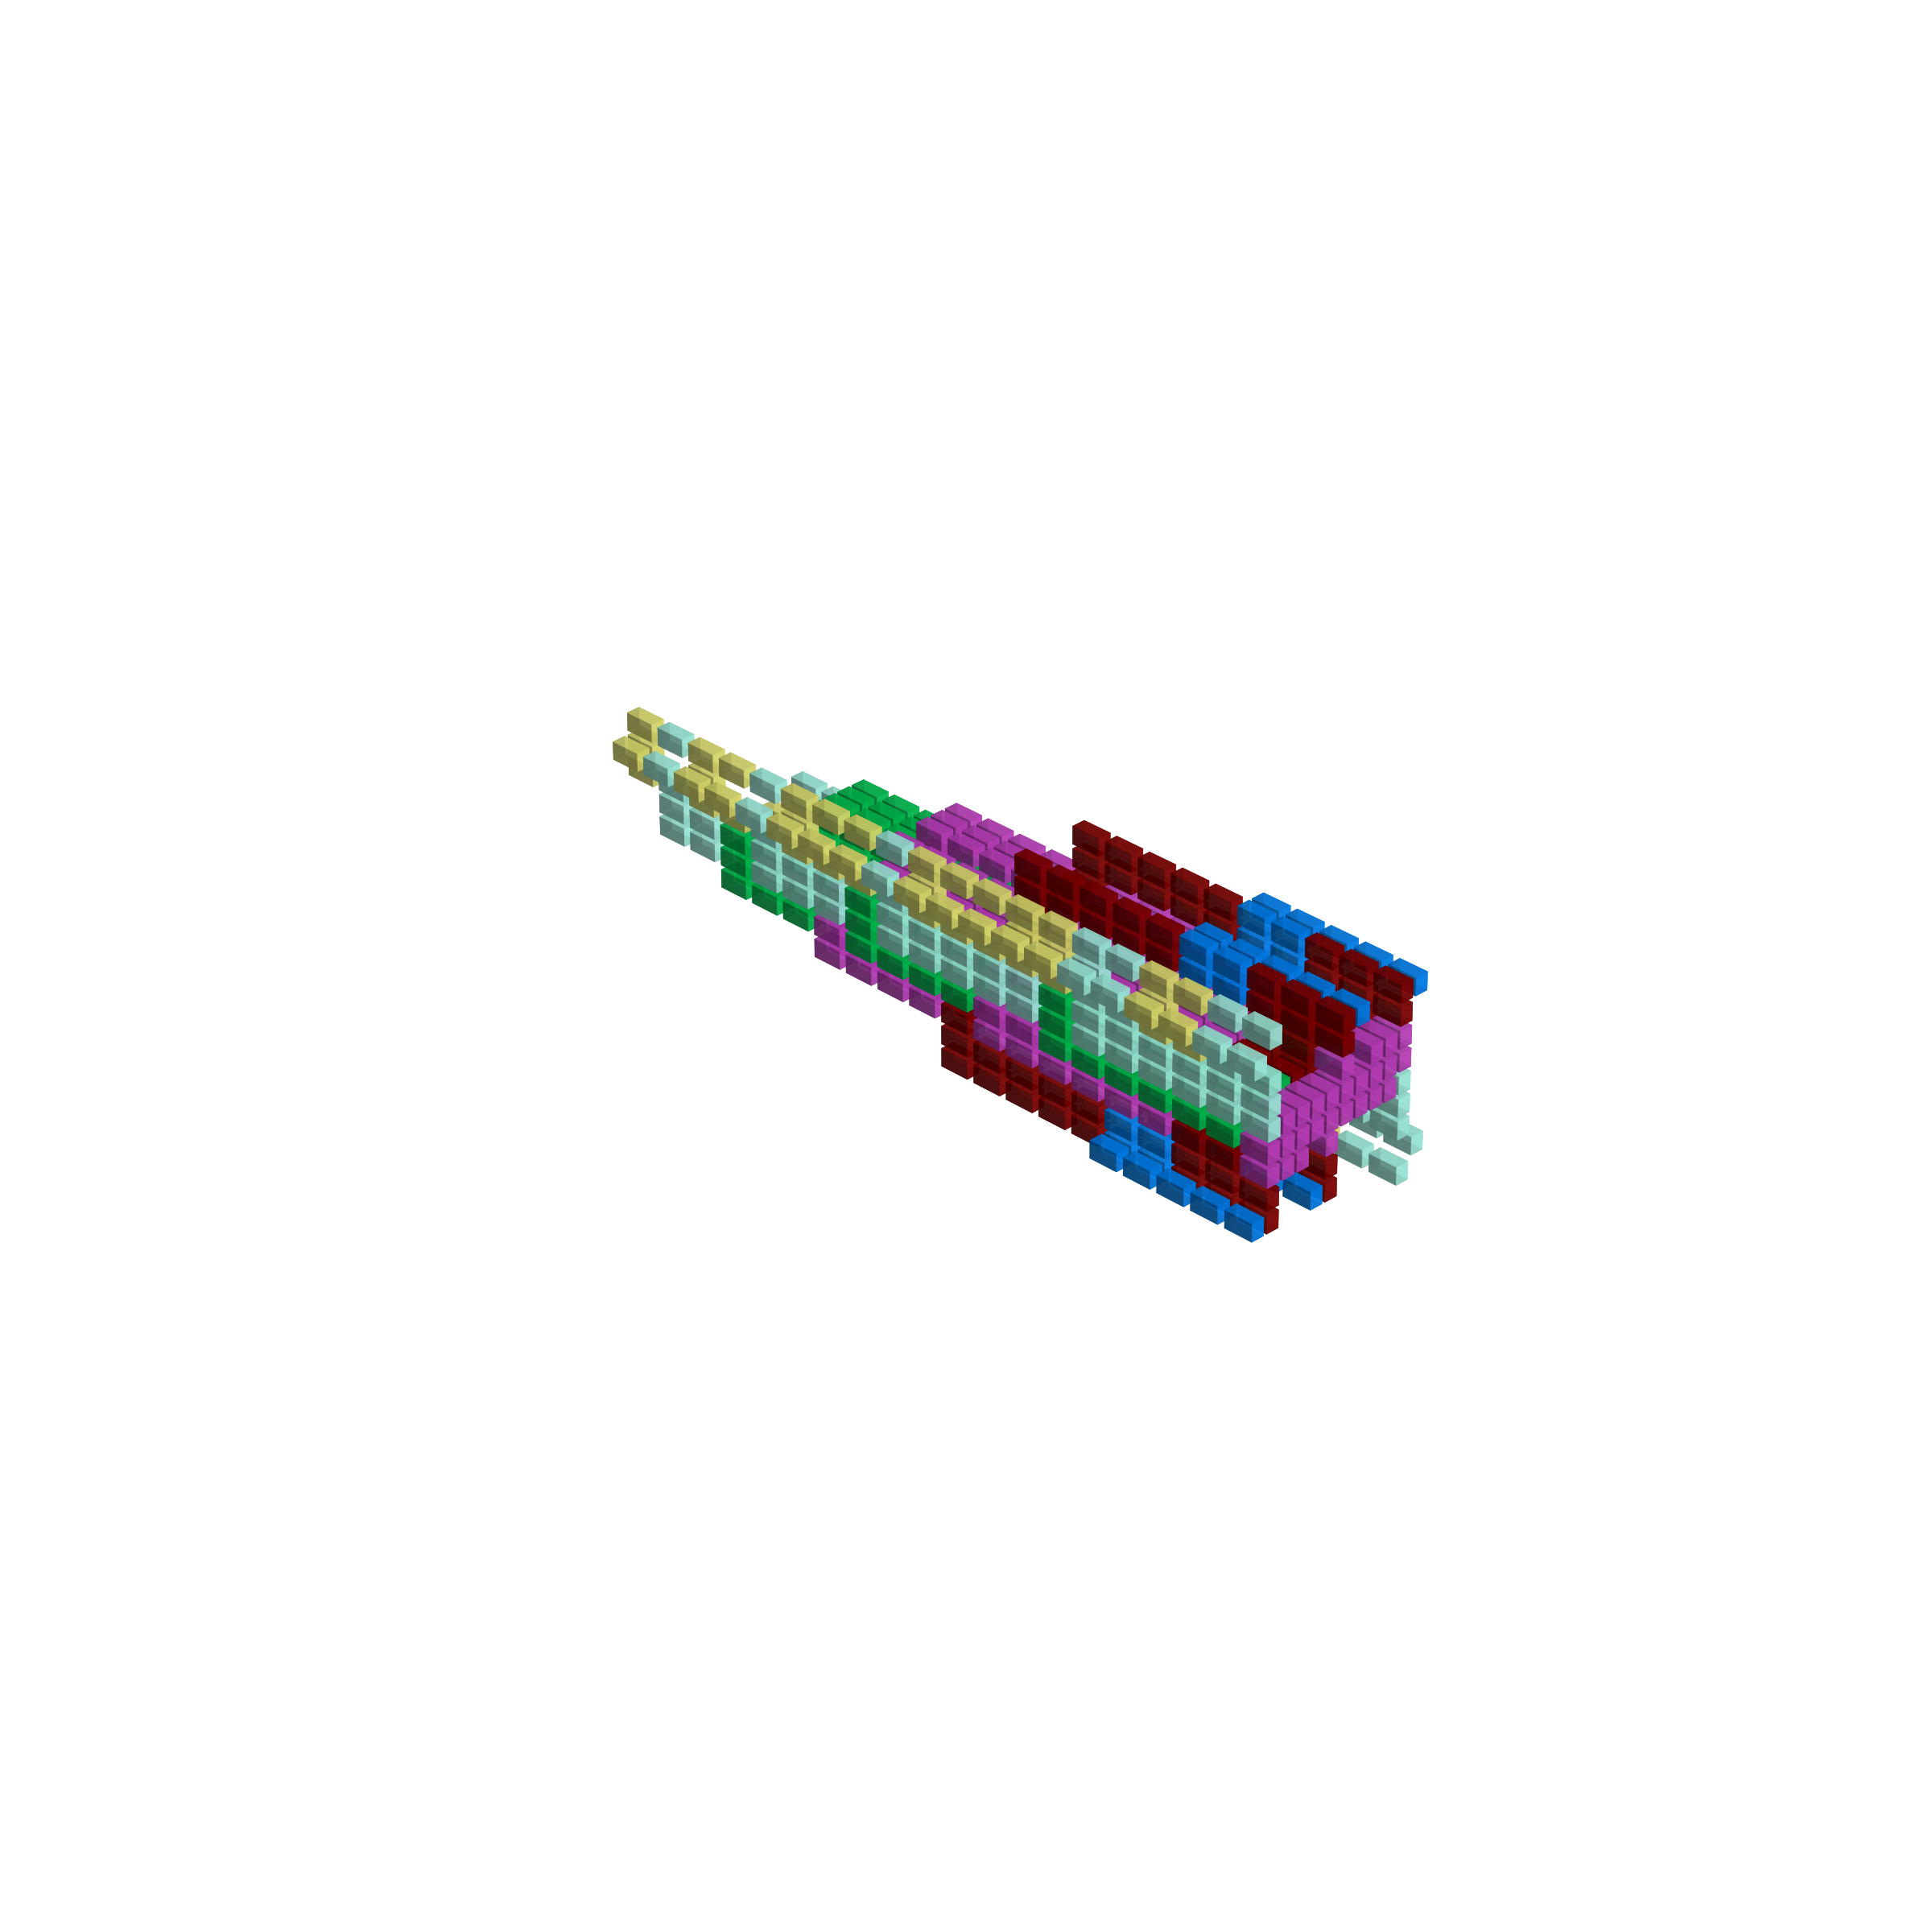
\includegraphics[width=8cm]{src/symmetries/pattern2_2-45.png}\\
        \vspace*{-5cm}
        \hspace*{-3cm}
        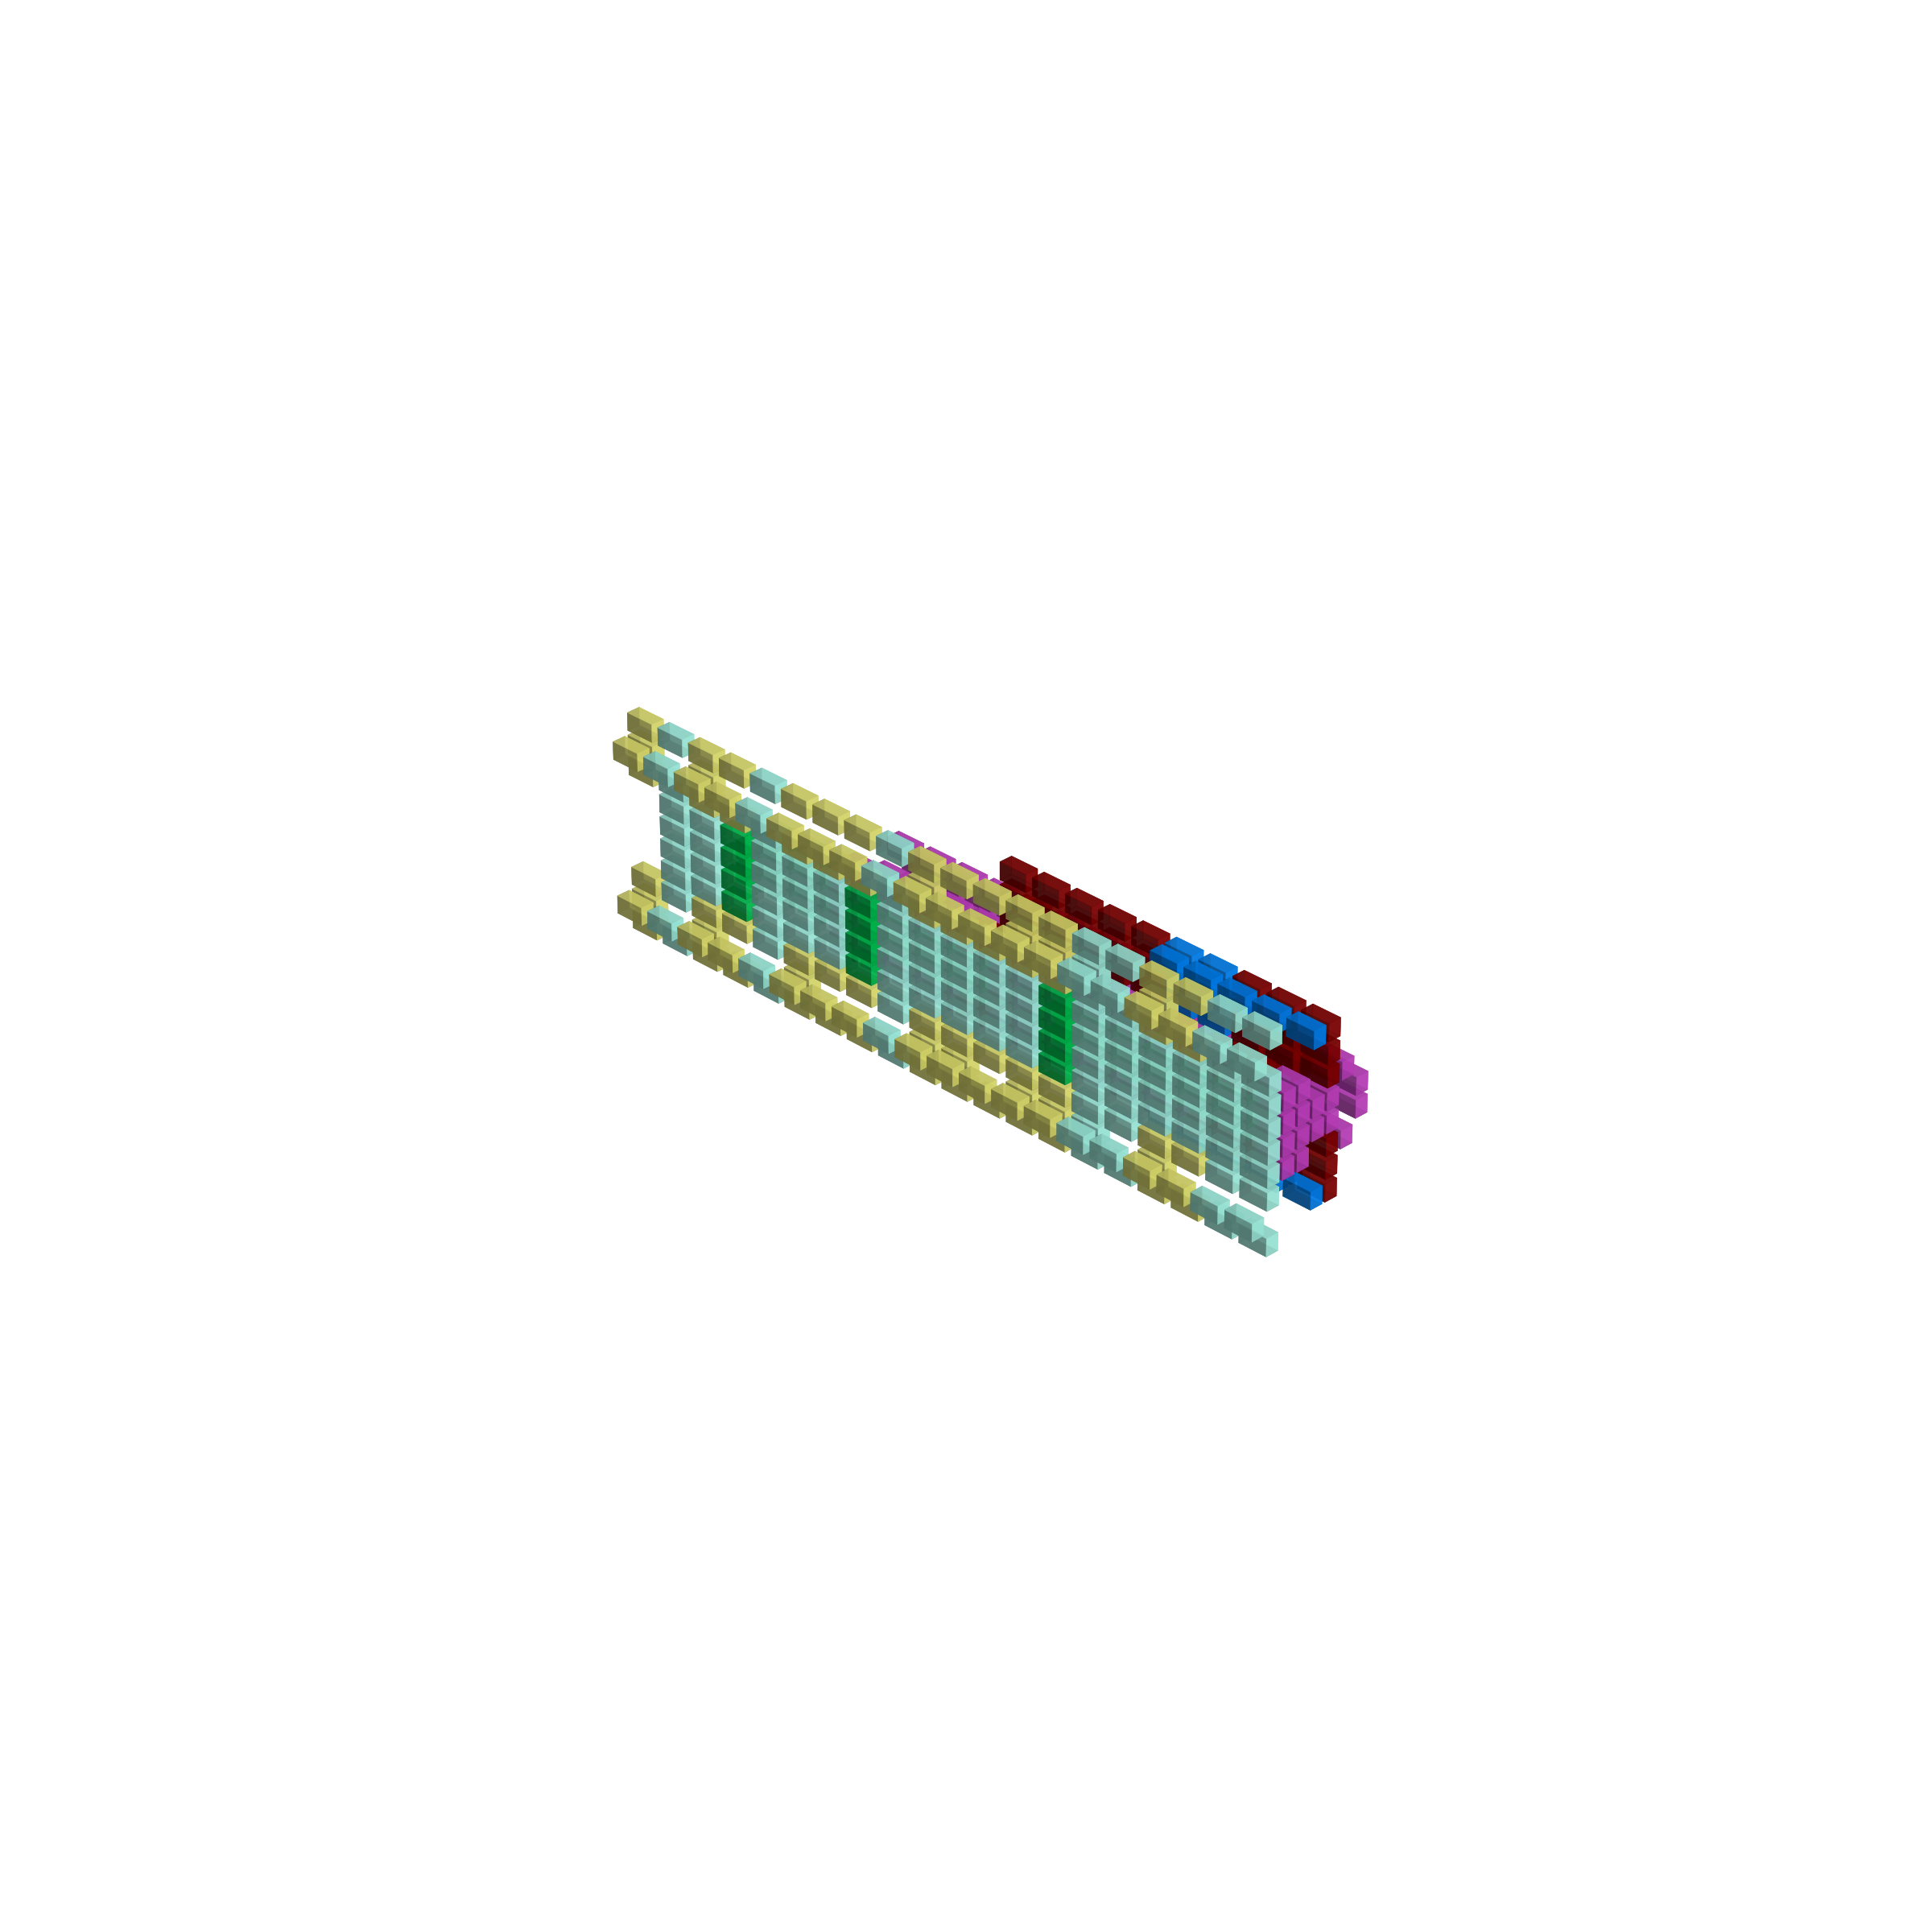
\includegraphics[width=8cm]{src/symmetries/pattern2_3-45.png}\\
        \vspace*{-8cm}
        \hspace*{2cm}
        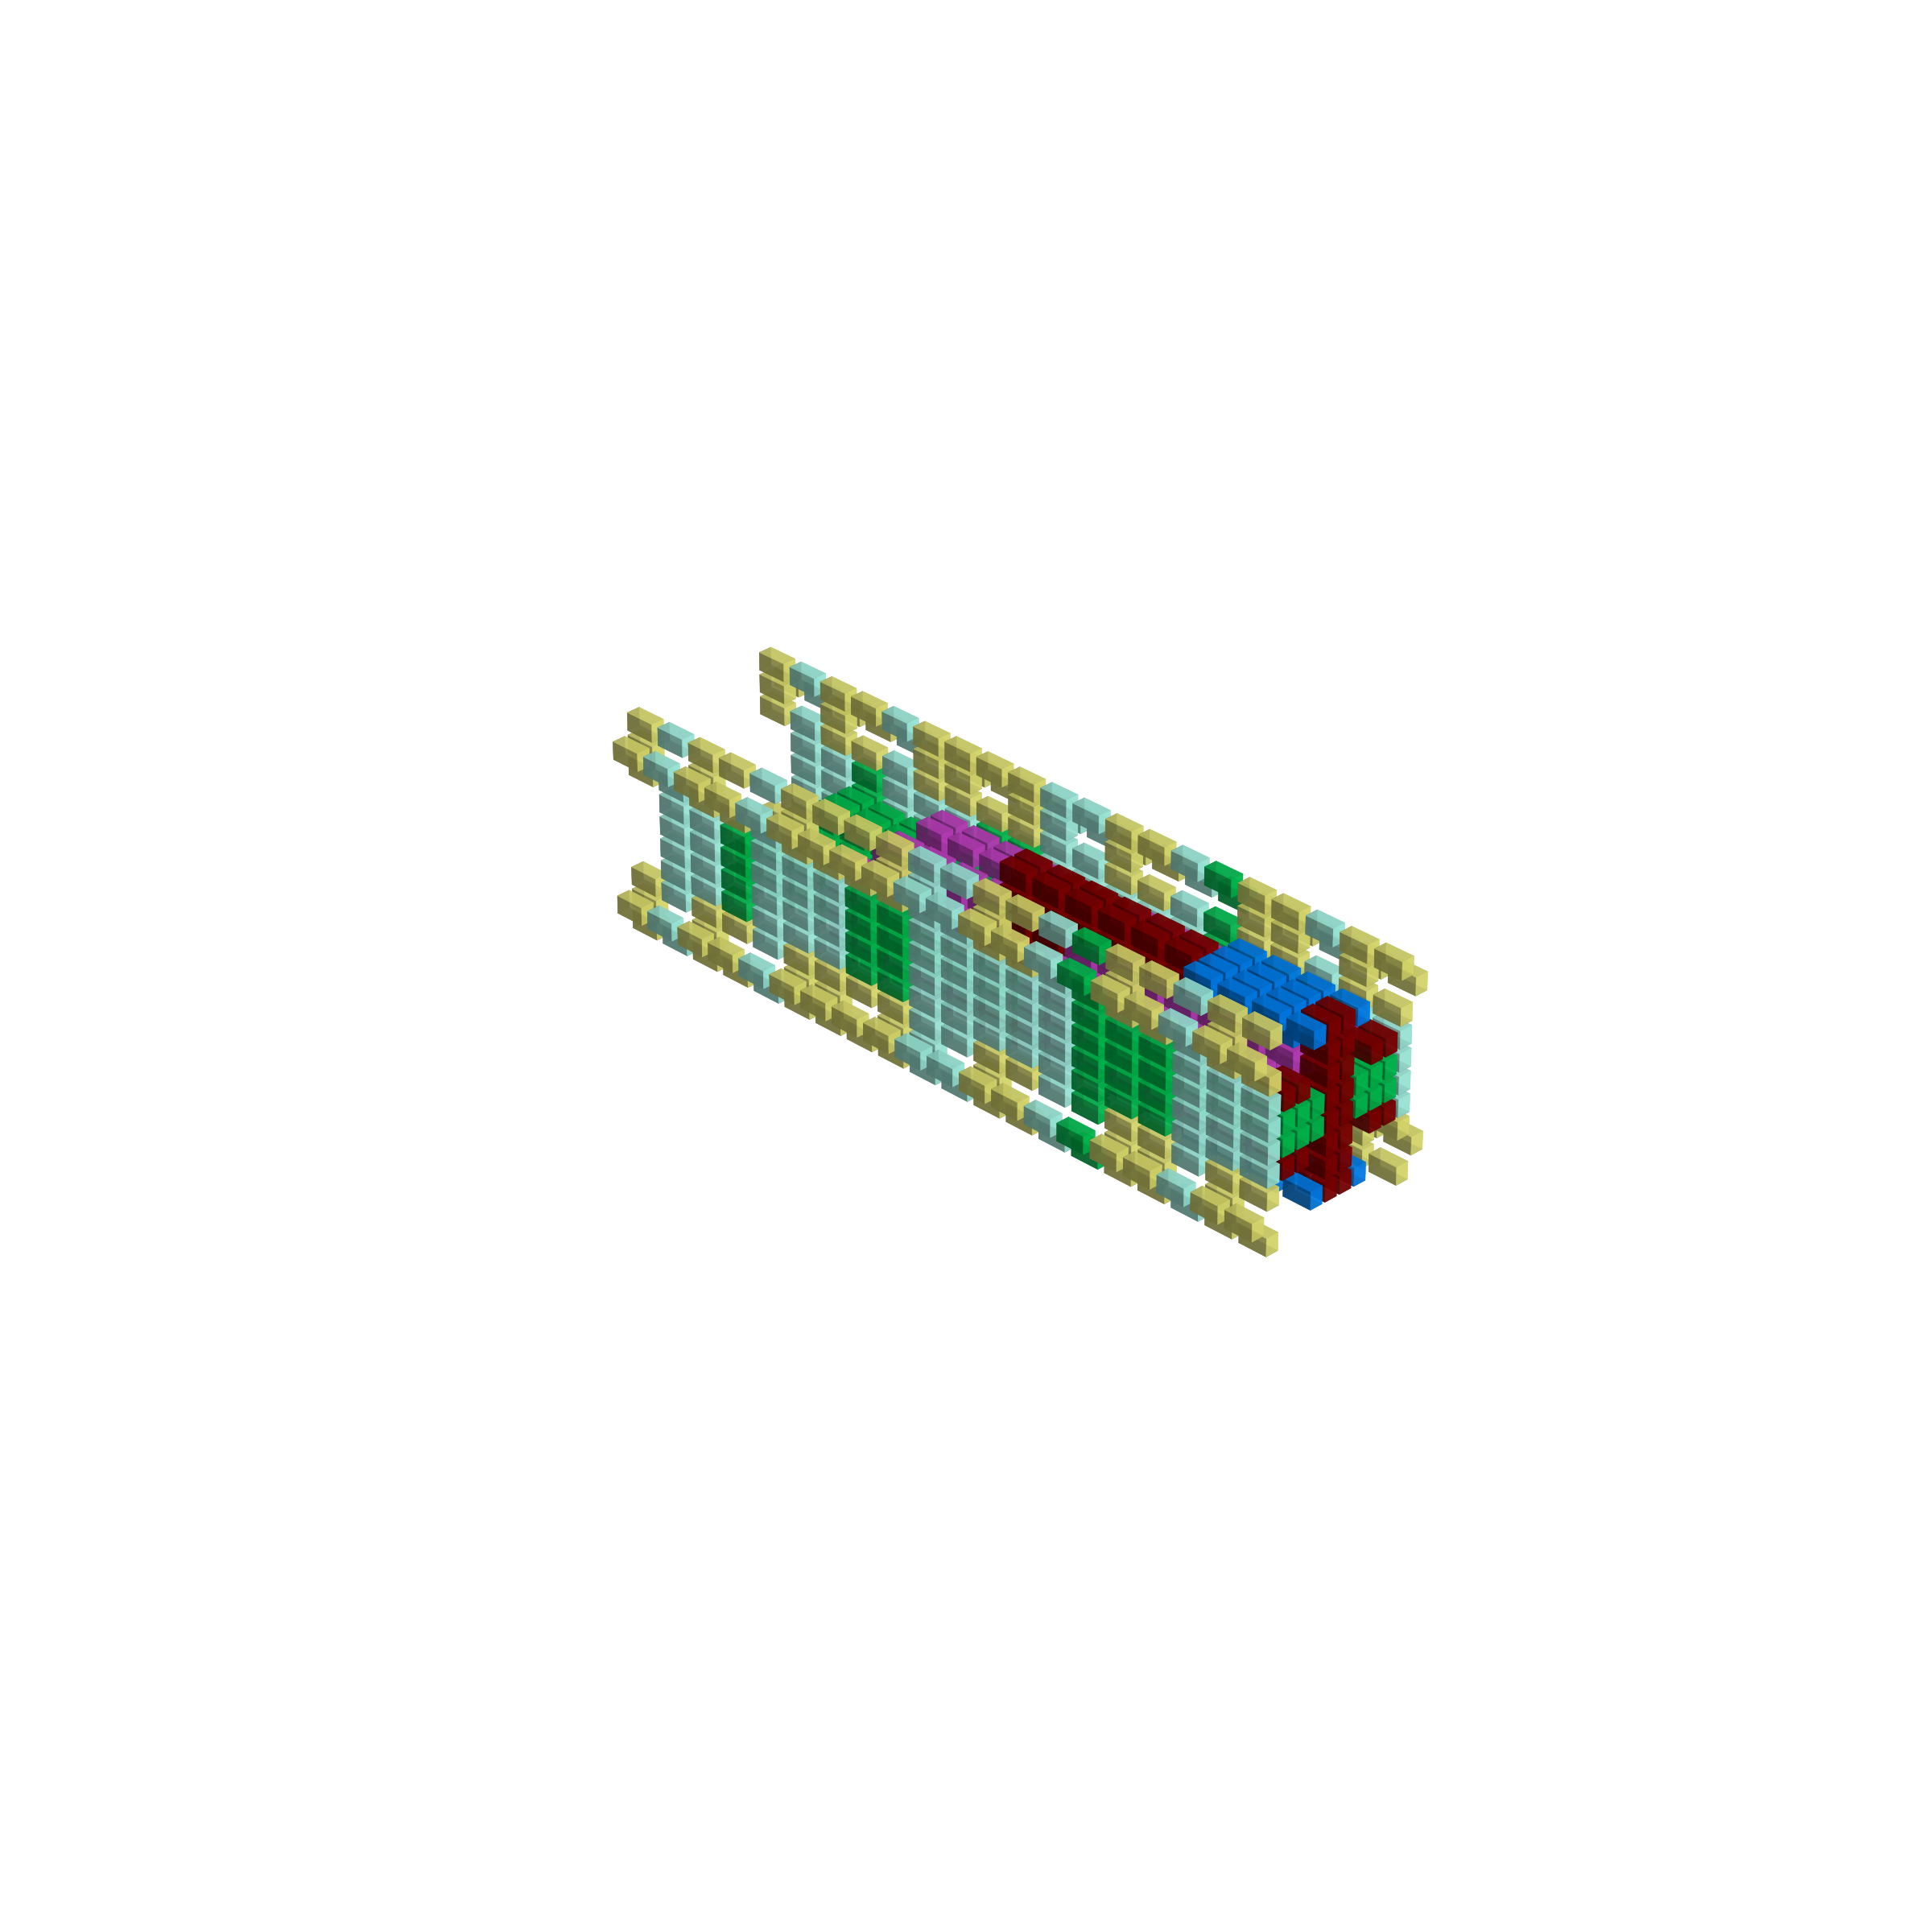
\includegraphics[width=8cm]{src/symmetries/pattern2_4-45.png}
        \vspace*{-2.5cm}
  \caption*{\getItem{2}}
  \end{figure}
\end{minipage}
\hspace{1cm}
\begin{minipage}[b]{0.50\linewidth}                                       
  \begin{figure}[H]
      \centering
        \vspace*{-1cm}
        \hspace*{-2cm}
        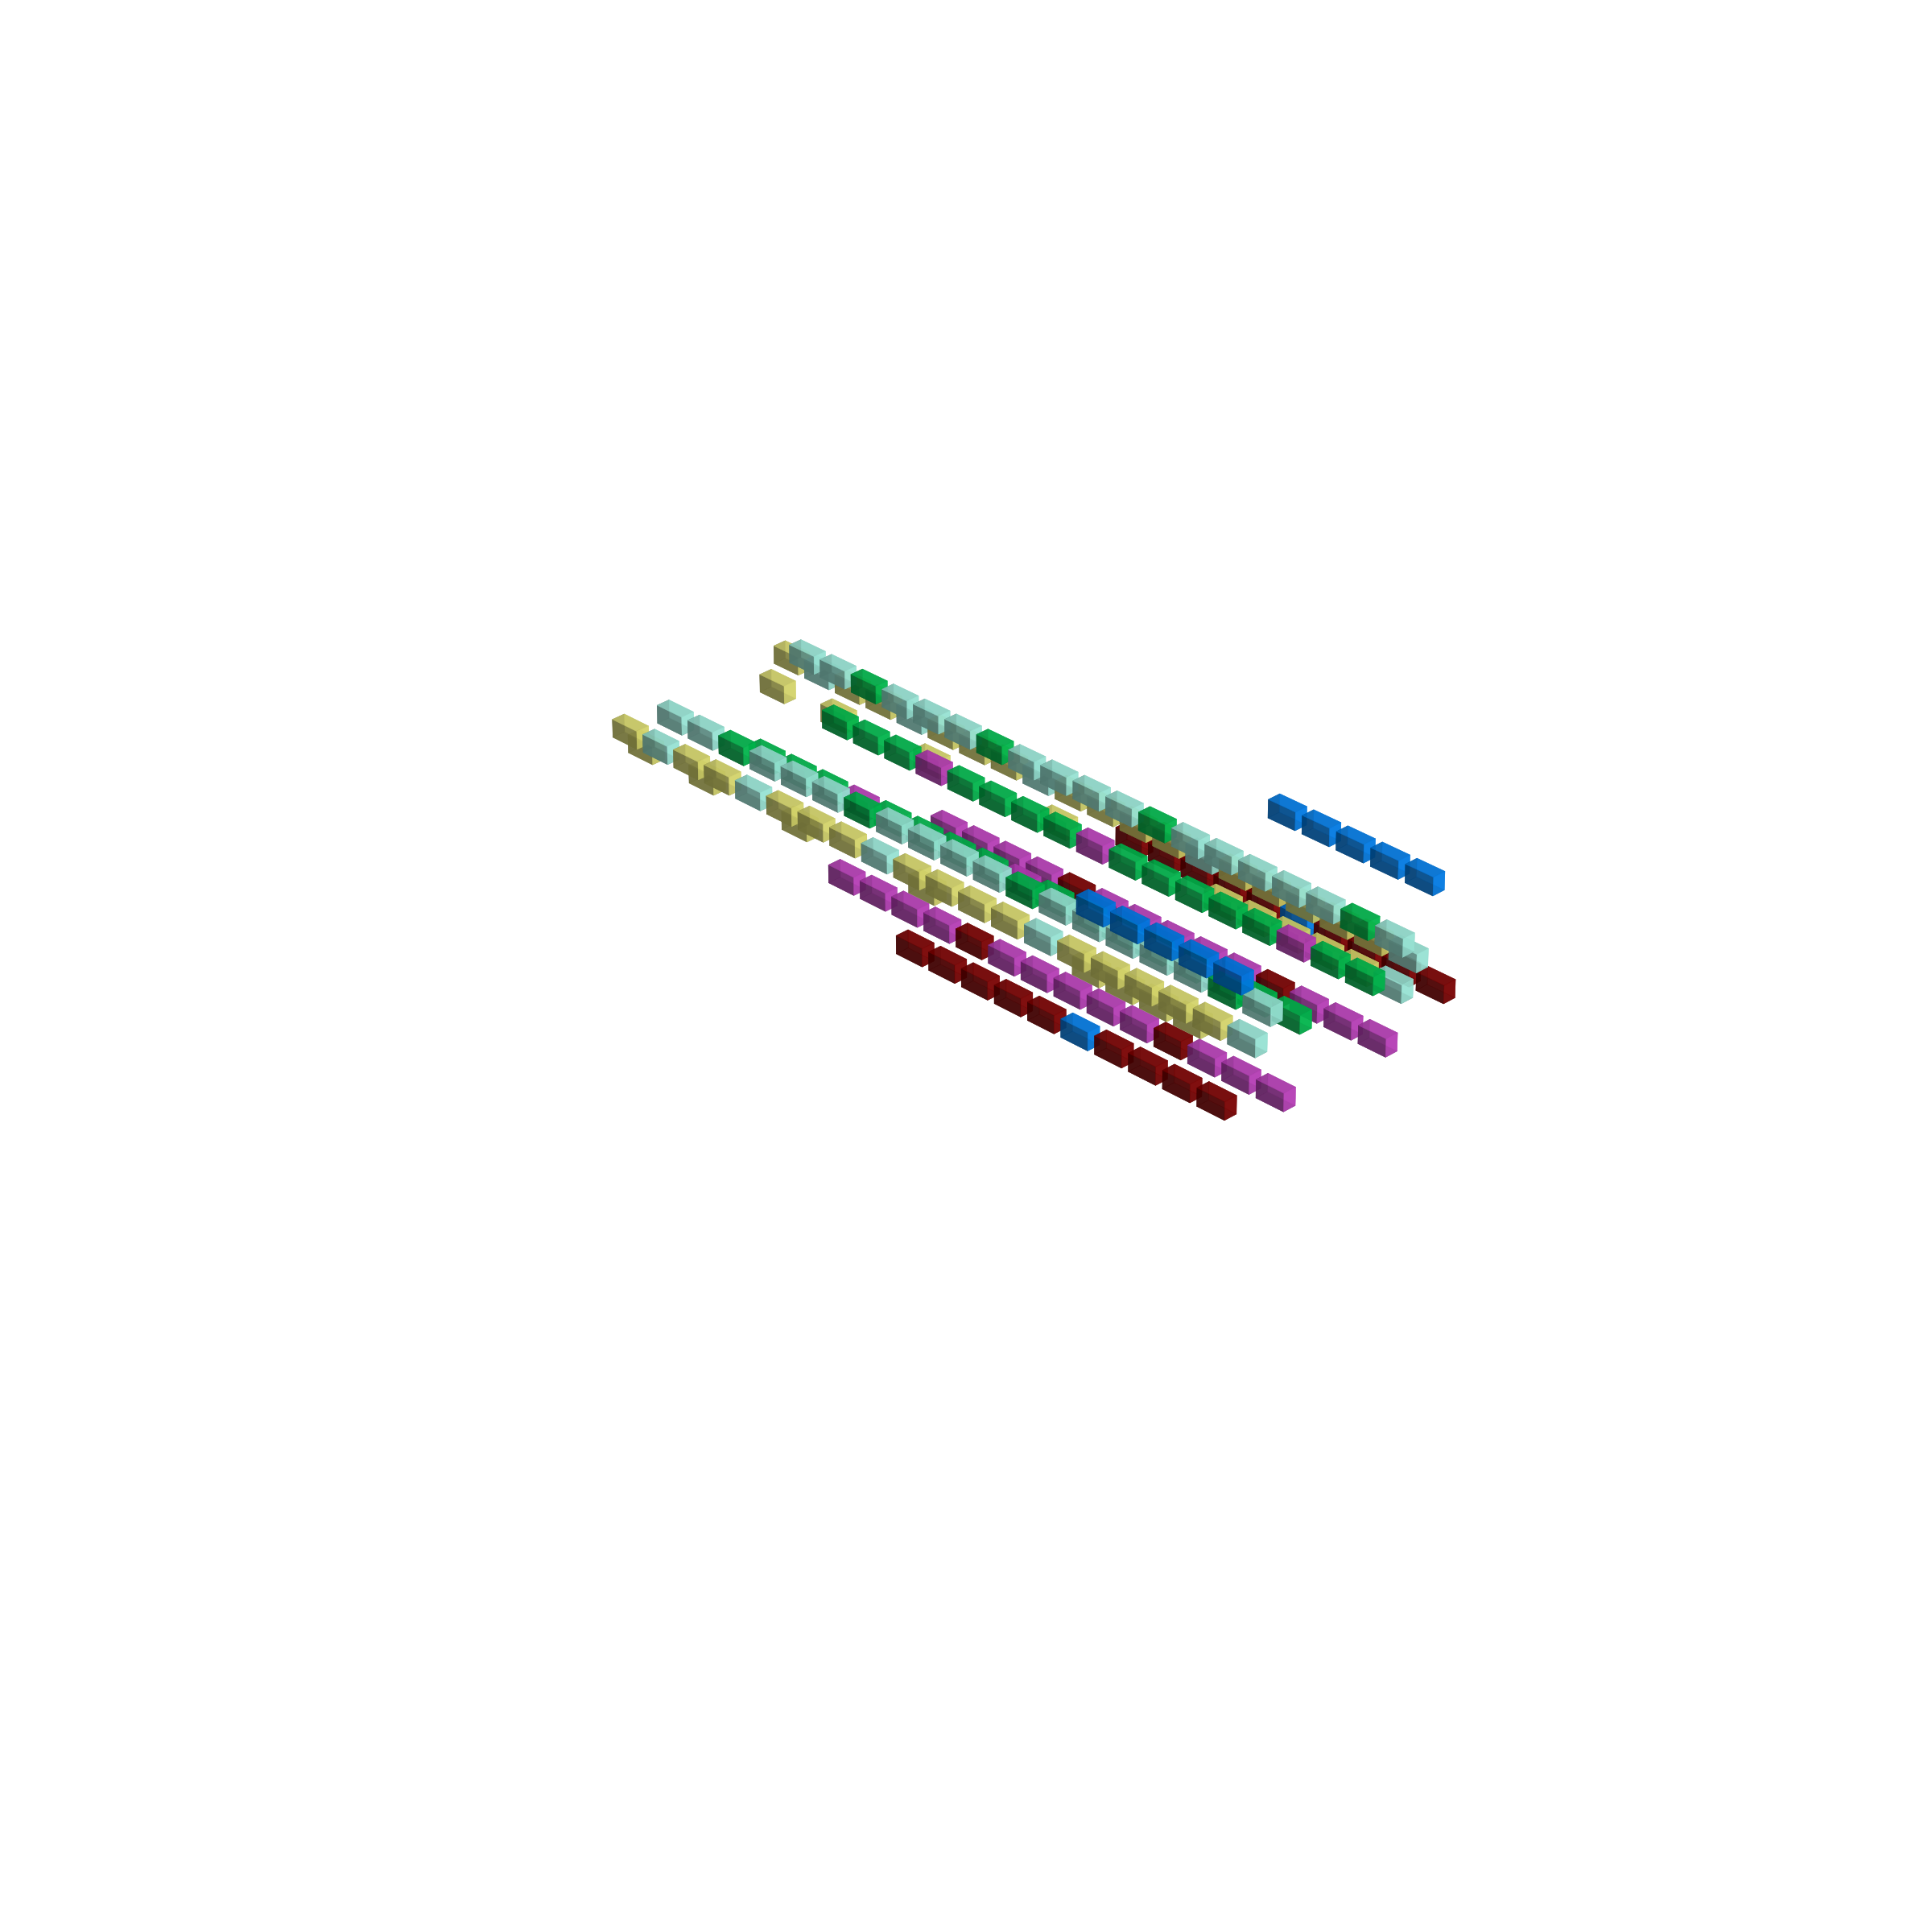
\includegraphics[width=8cm]{src/symmetries/pattern3_1-45.png}%
        \hspace*{-4cm}
        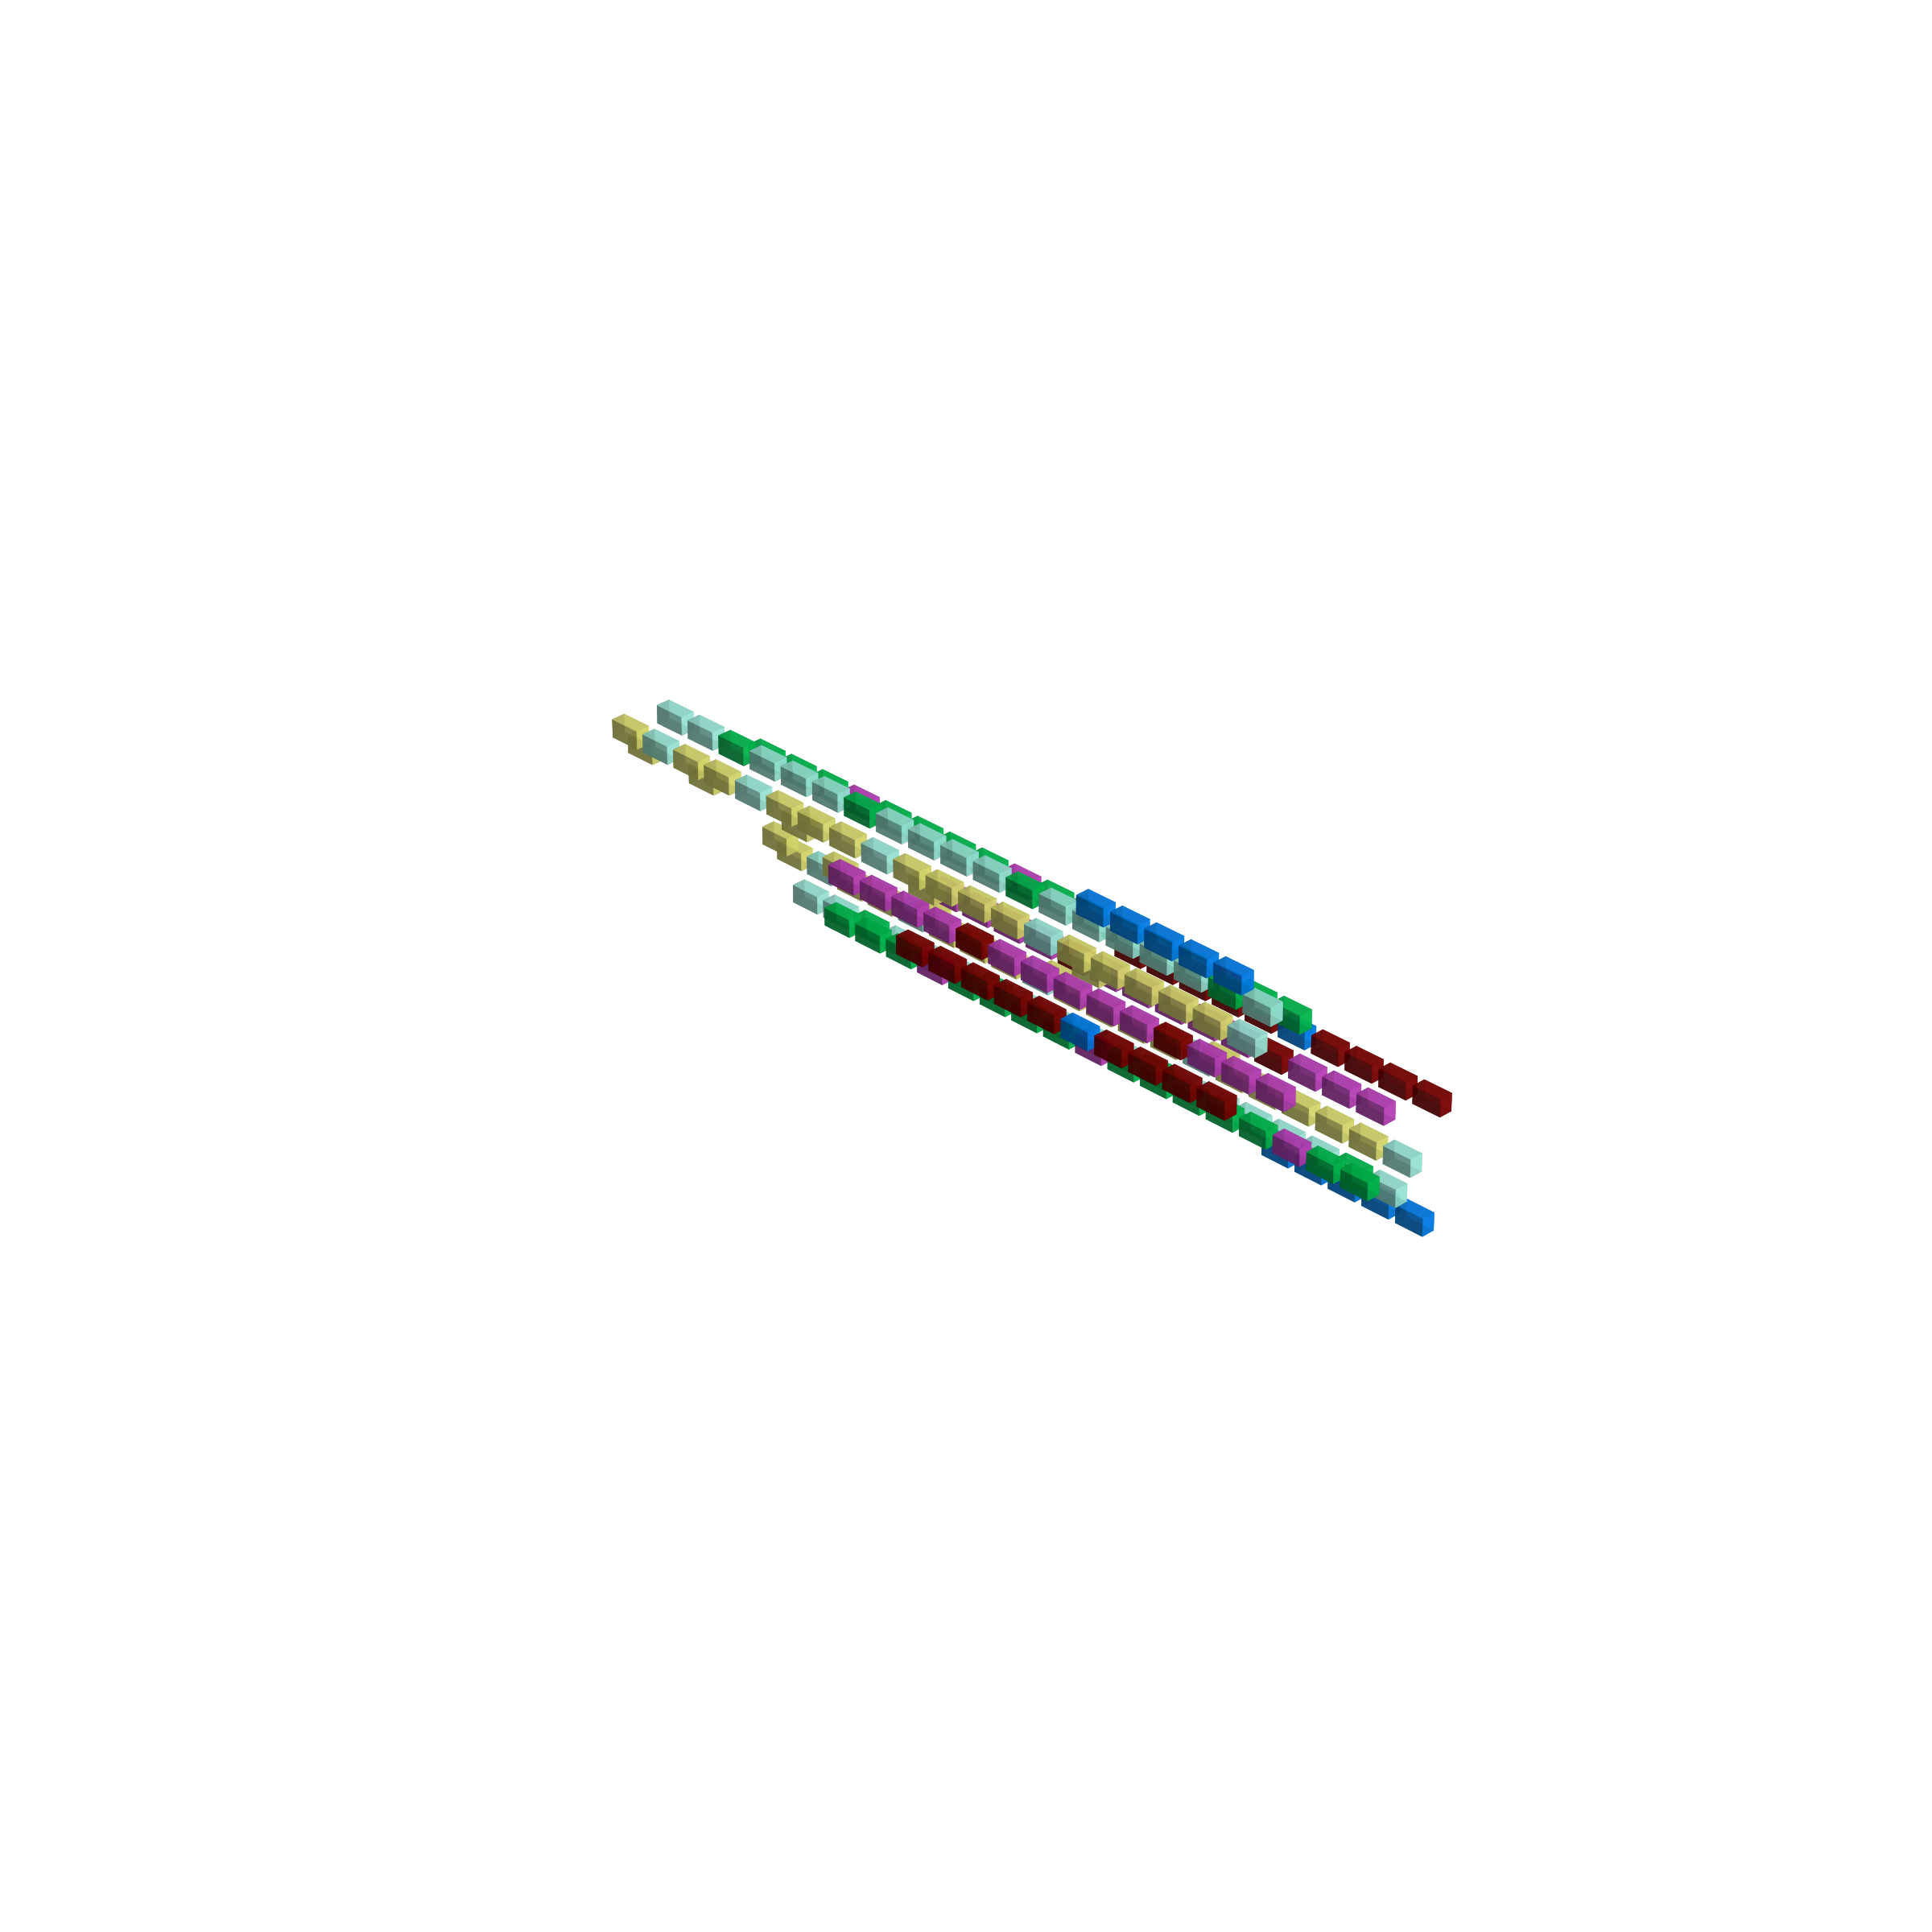
\includegraphics[width=8cm]{src/symmetries/pattern3_2-45.png}\\
        \vspace*{-5cm}
        \hspace*{-1cm}
        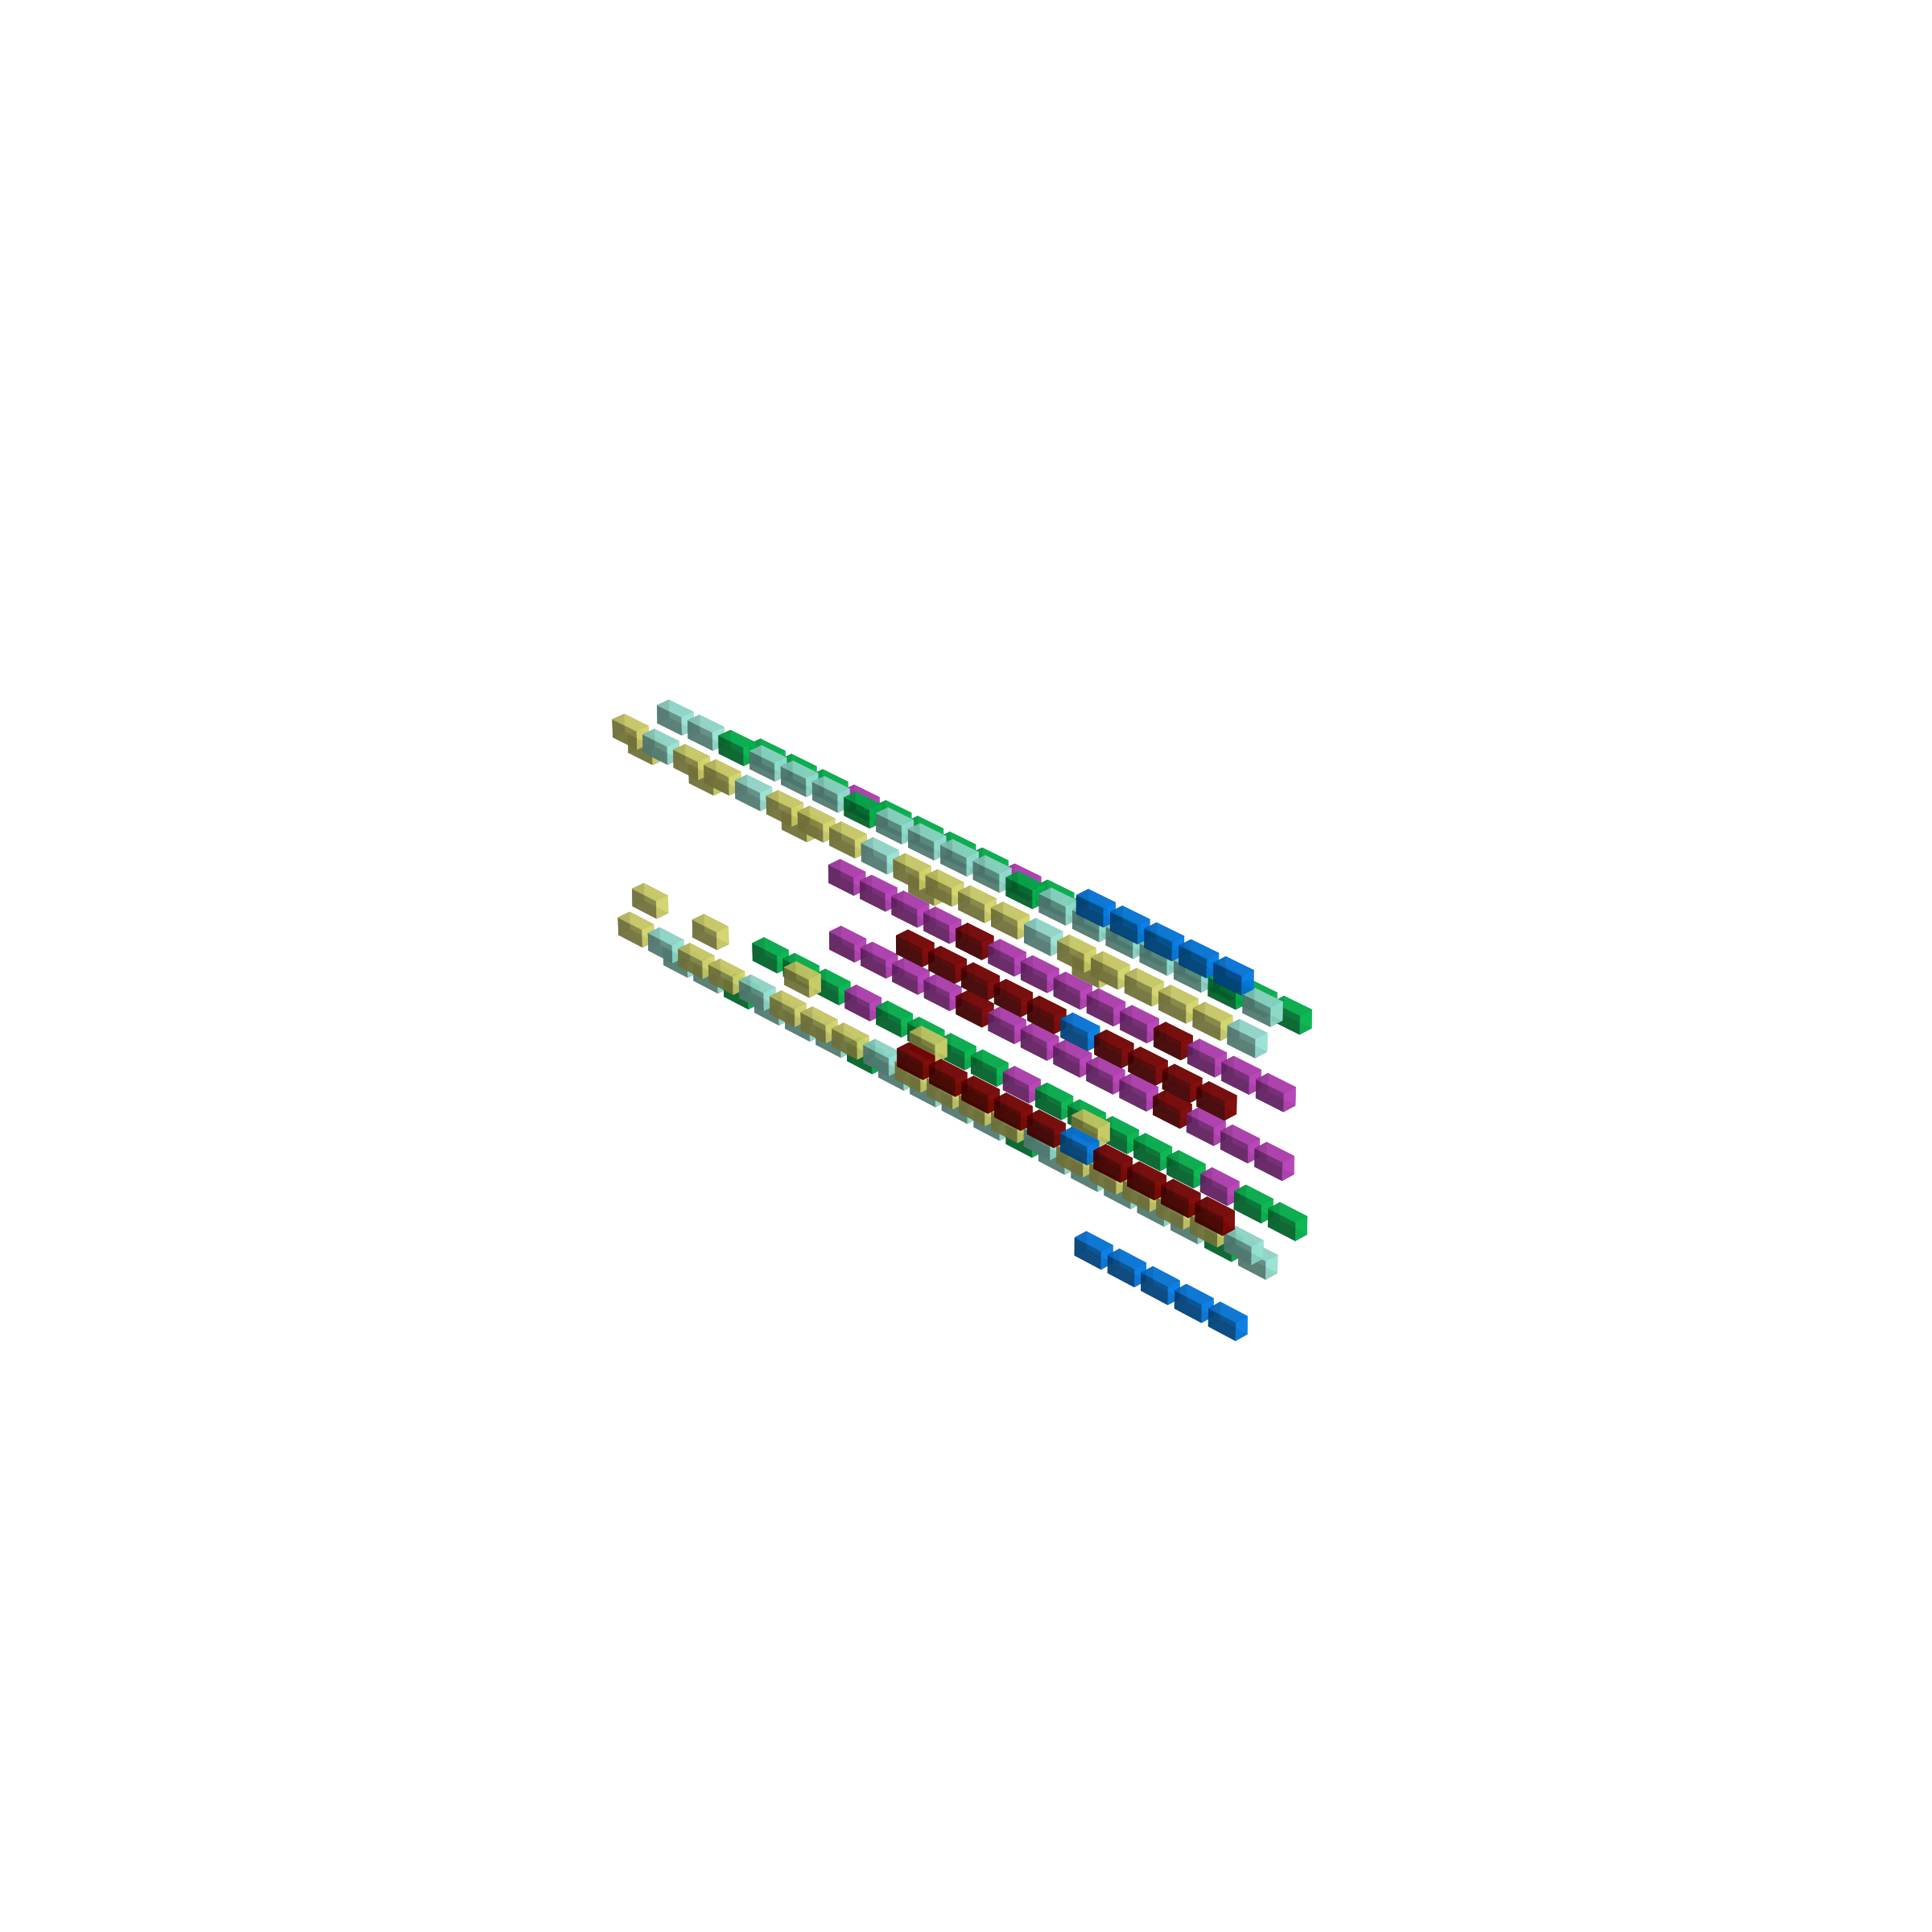
\includegraphics[width=8cm]{src/symmetries/pattern3_3-45.png}\\
        \vspace*{-8cm}
        \hspace*{2cm}
        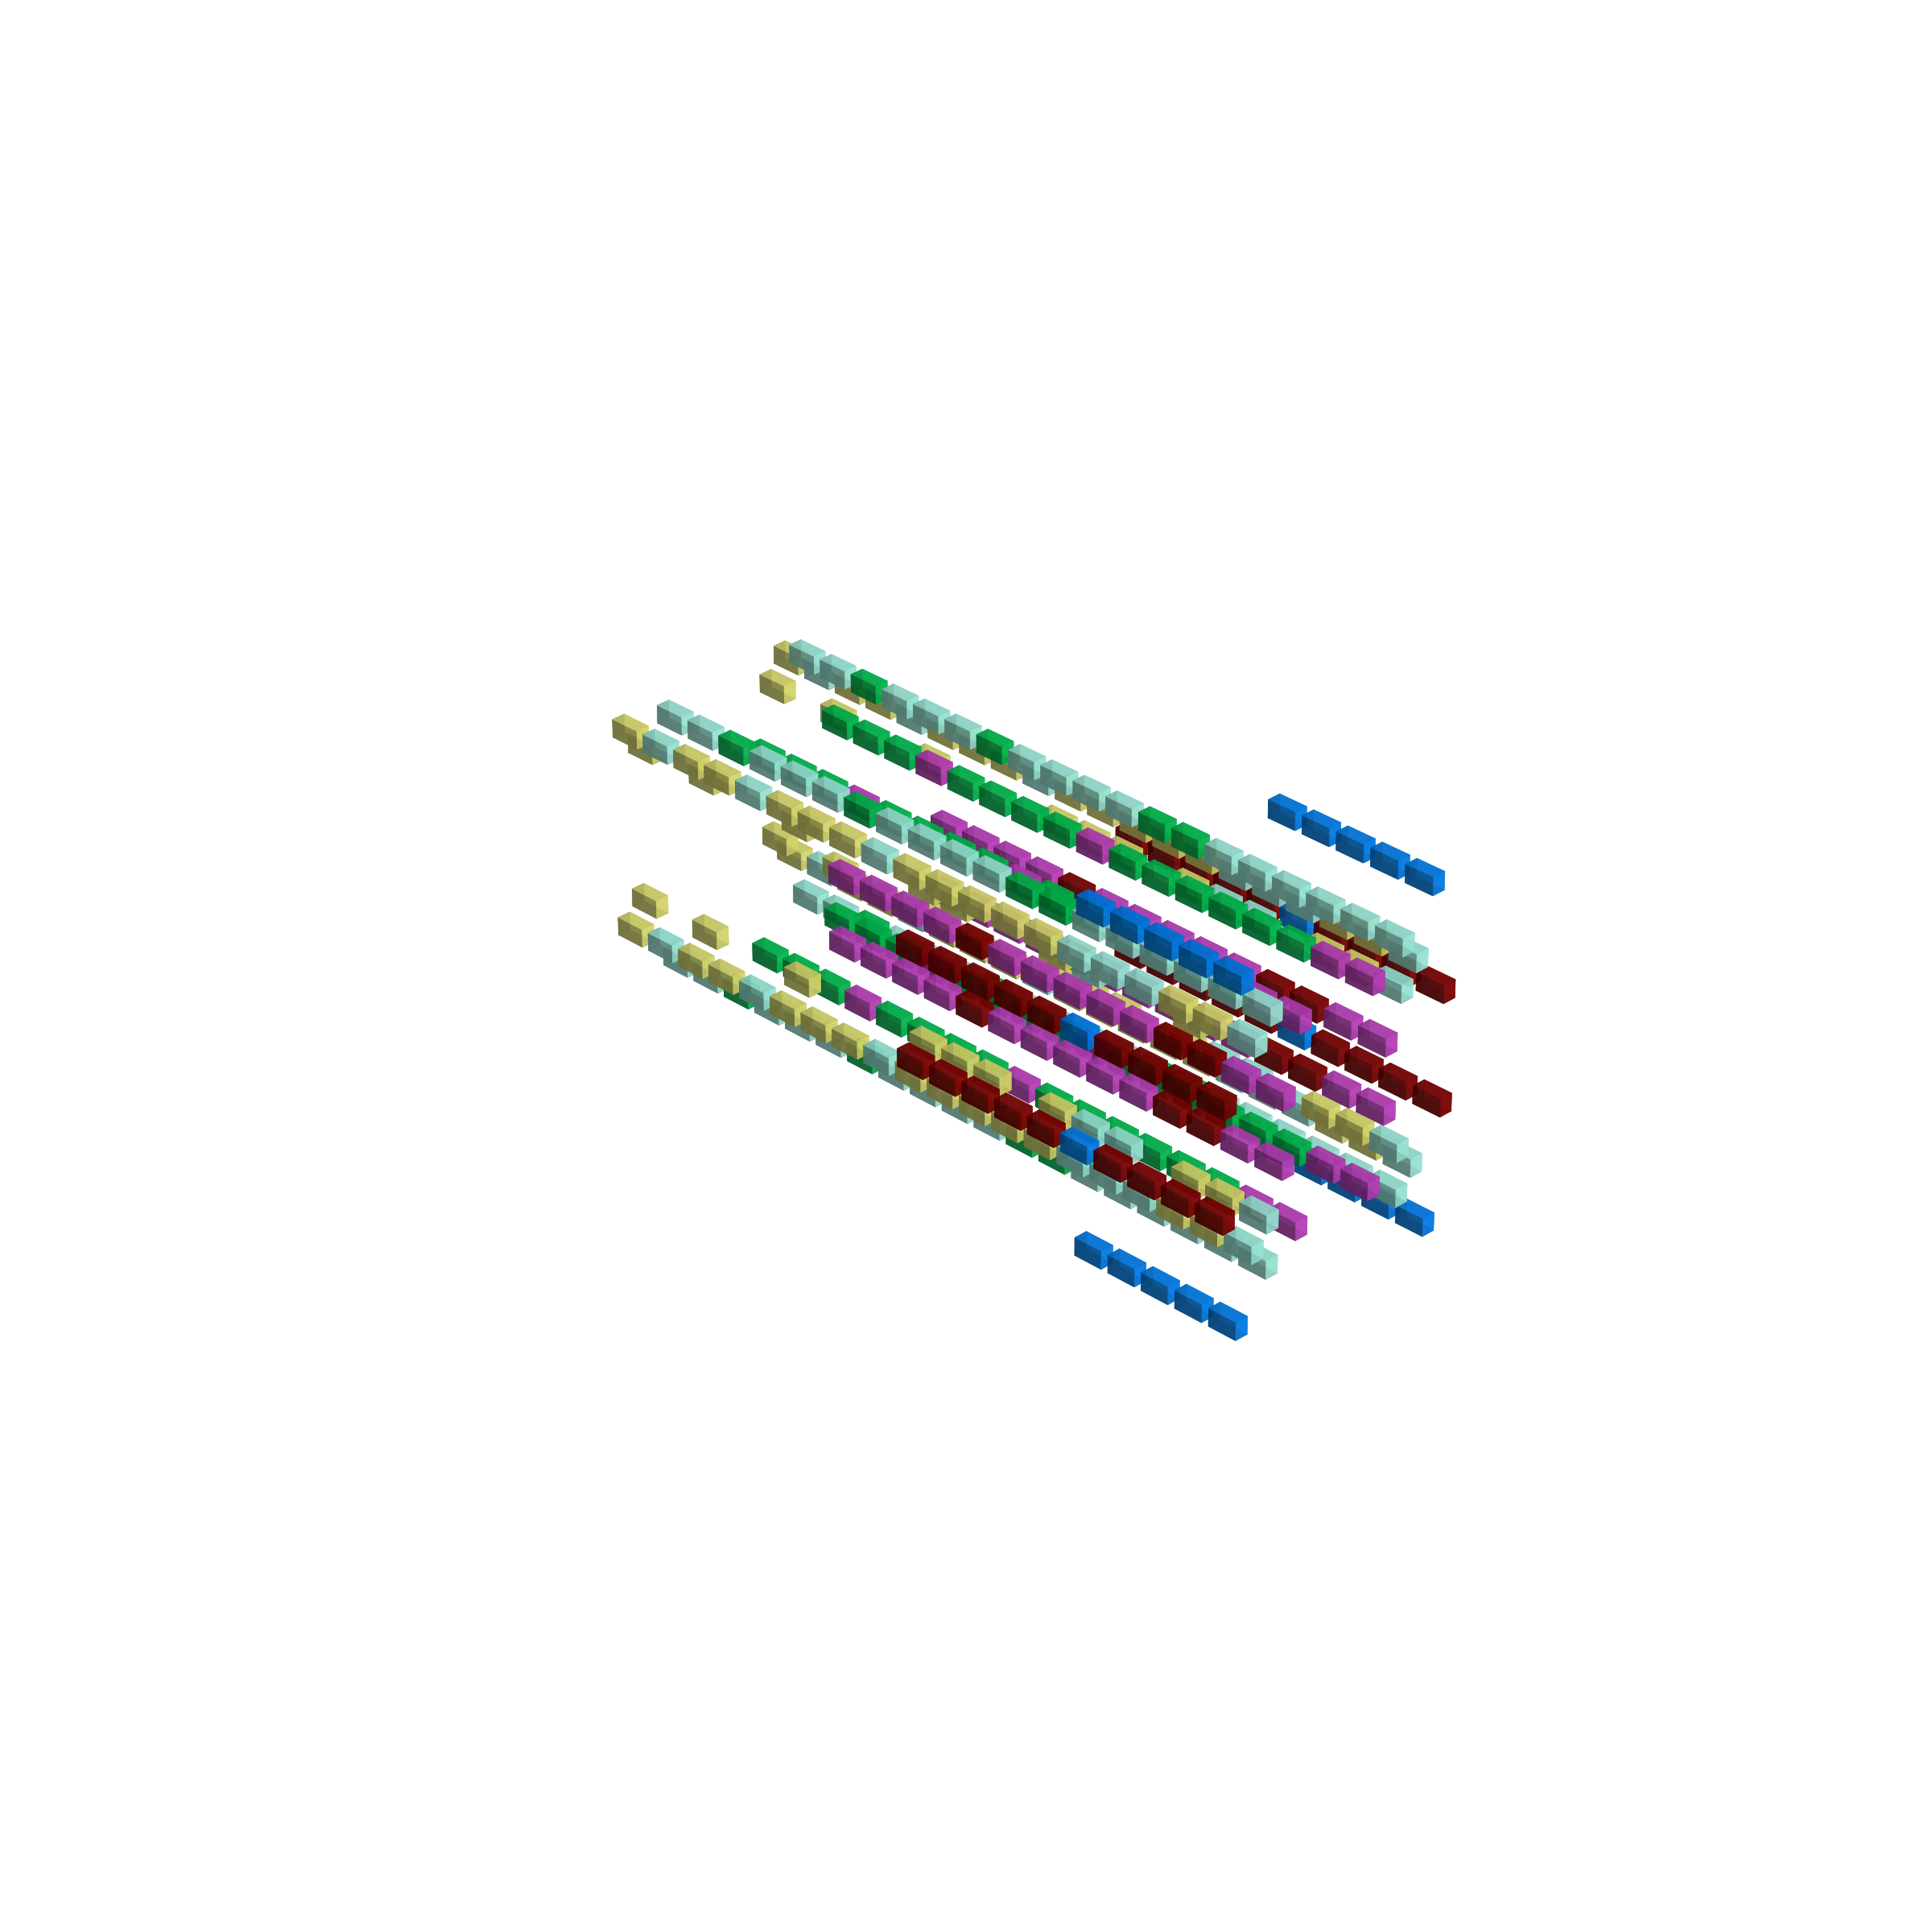
\includegraphics[width=8cm]{src/symmetries/pattern3_4-45.png}
        \vspace*{-2.5cm}
  \caption*{\getItem{3}}
  \end{figure}
\end{minipage}
\begin{minipage}[b]{0.50\linewidth}                                       
  \begin{figure}[H]
      \centering
        \vspace*{-1cm}
        \hspace*{-2cm}
        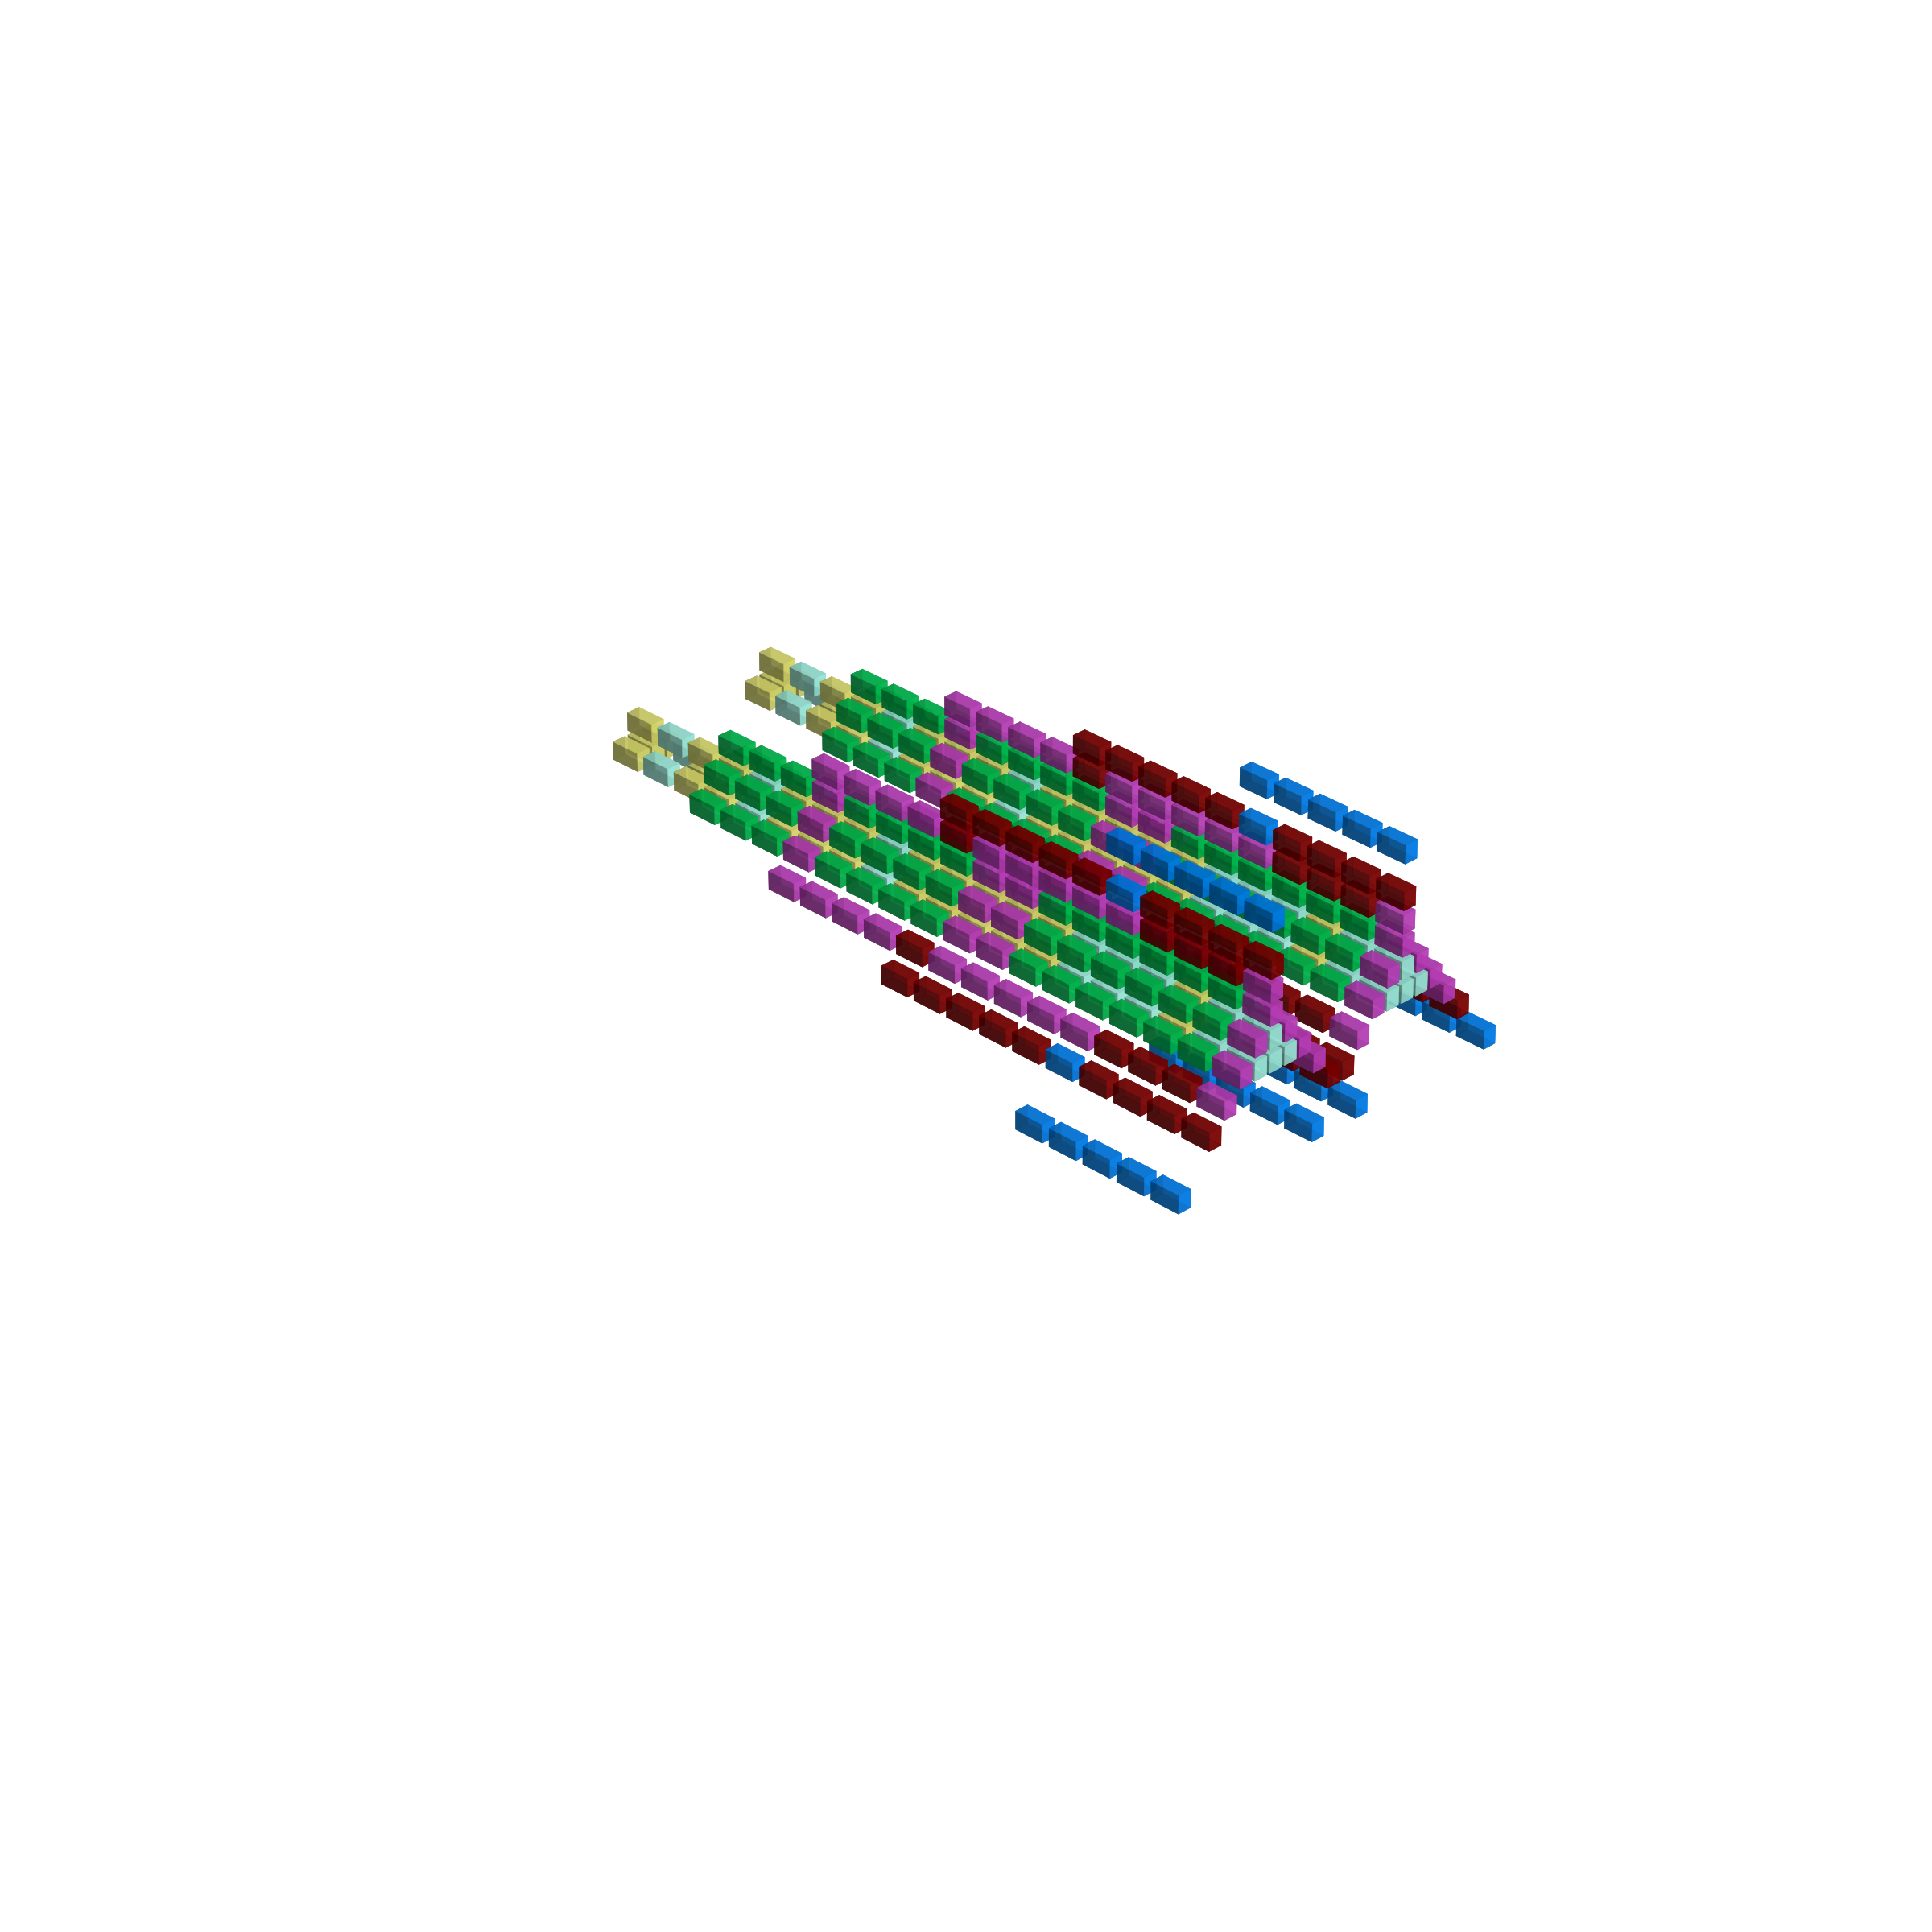
\includegraphics[width=8cm]{src/symmetries/pattern4_1-45.png}%
        \hspace*{-4cm}
        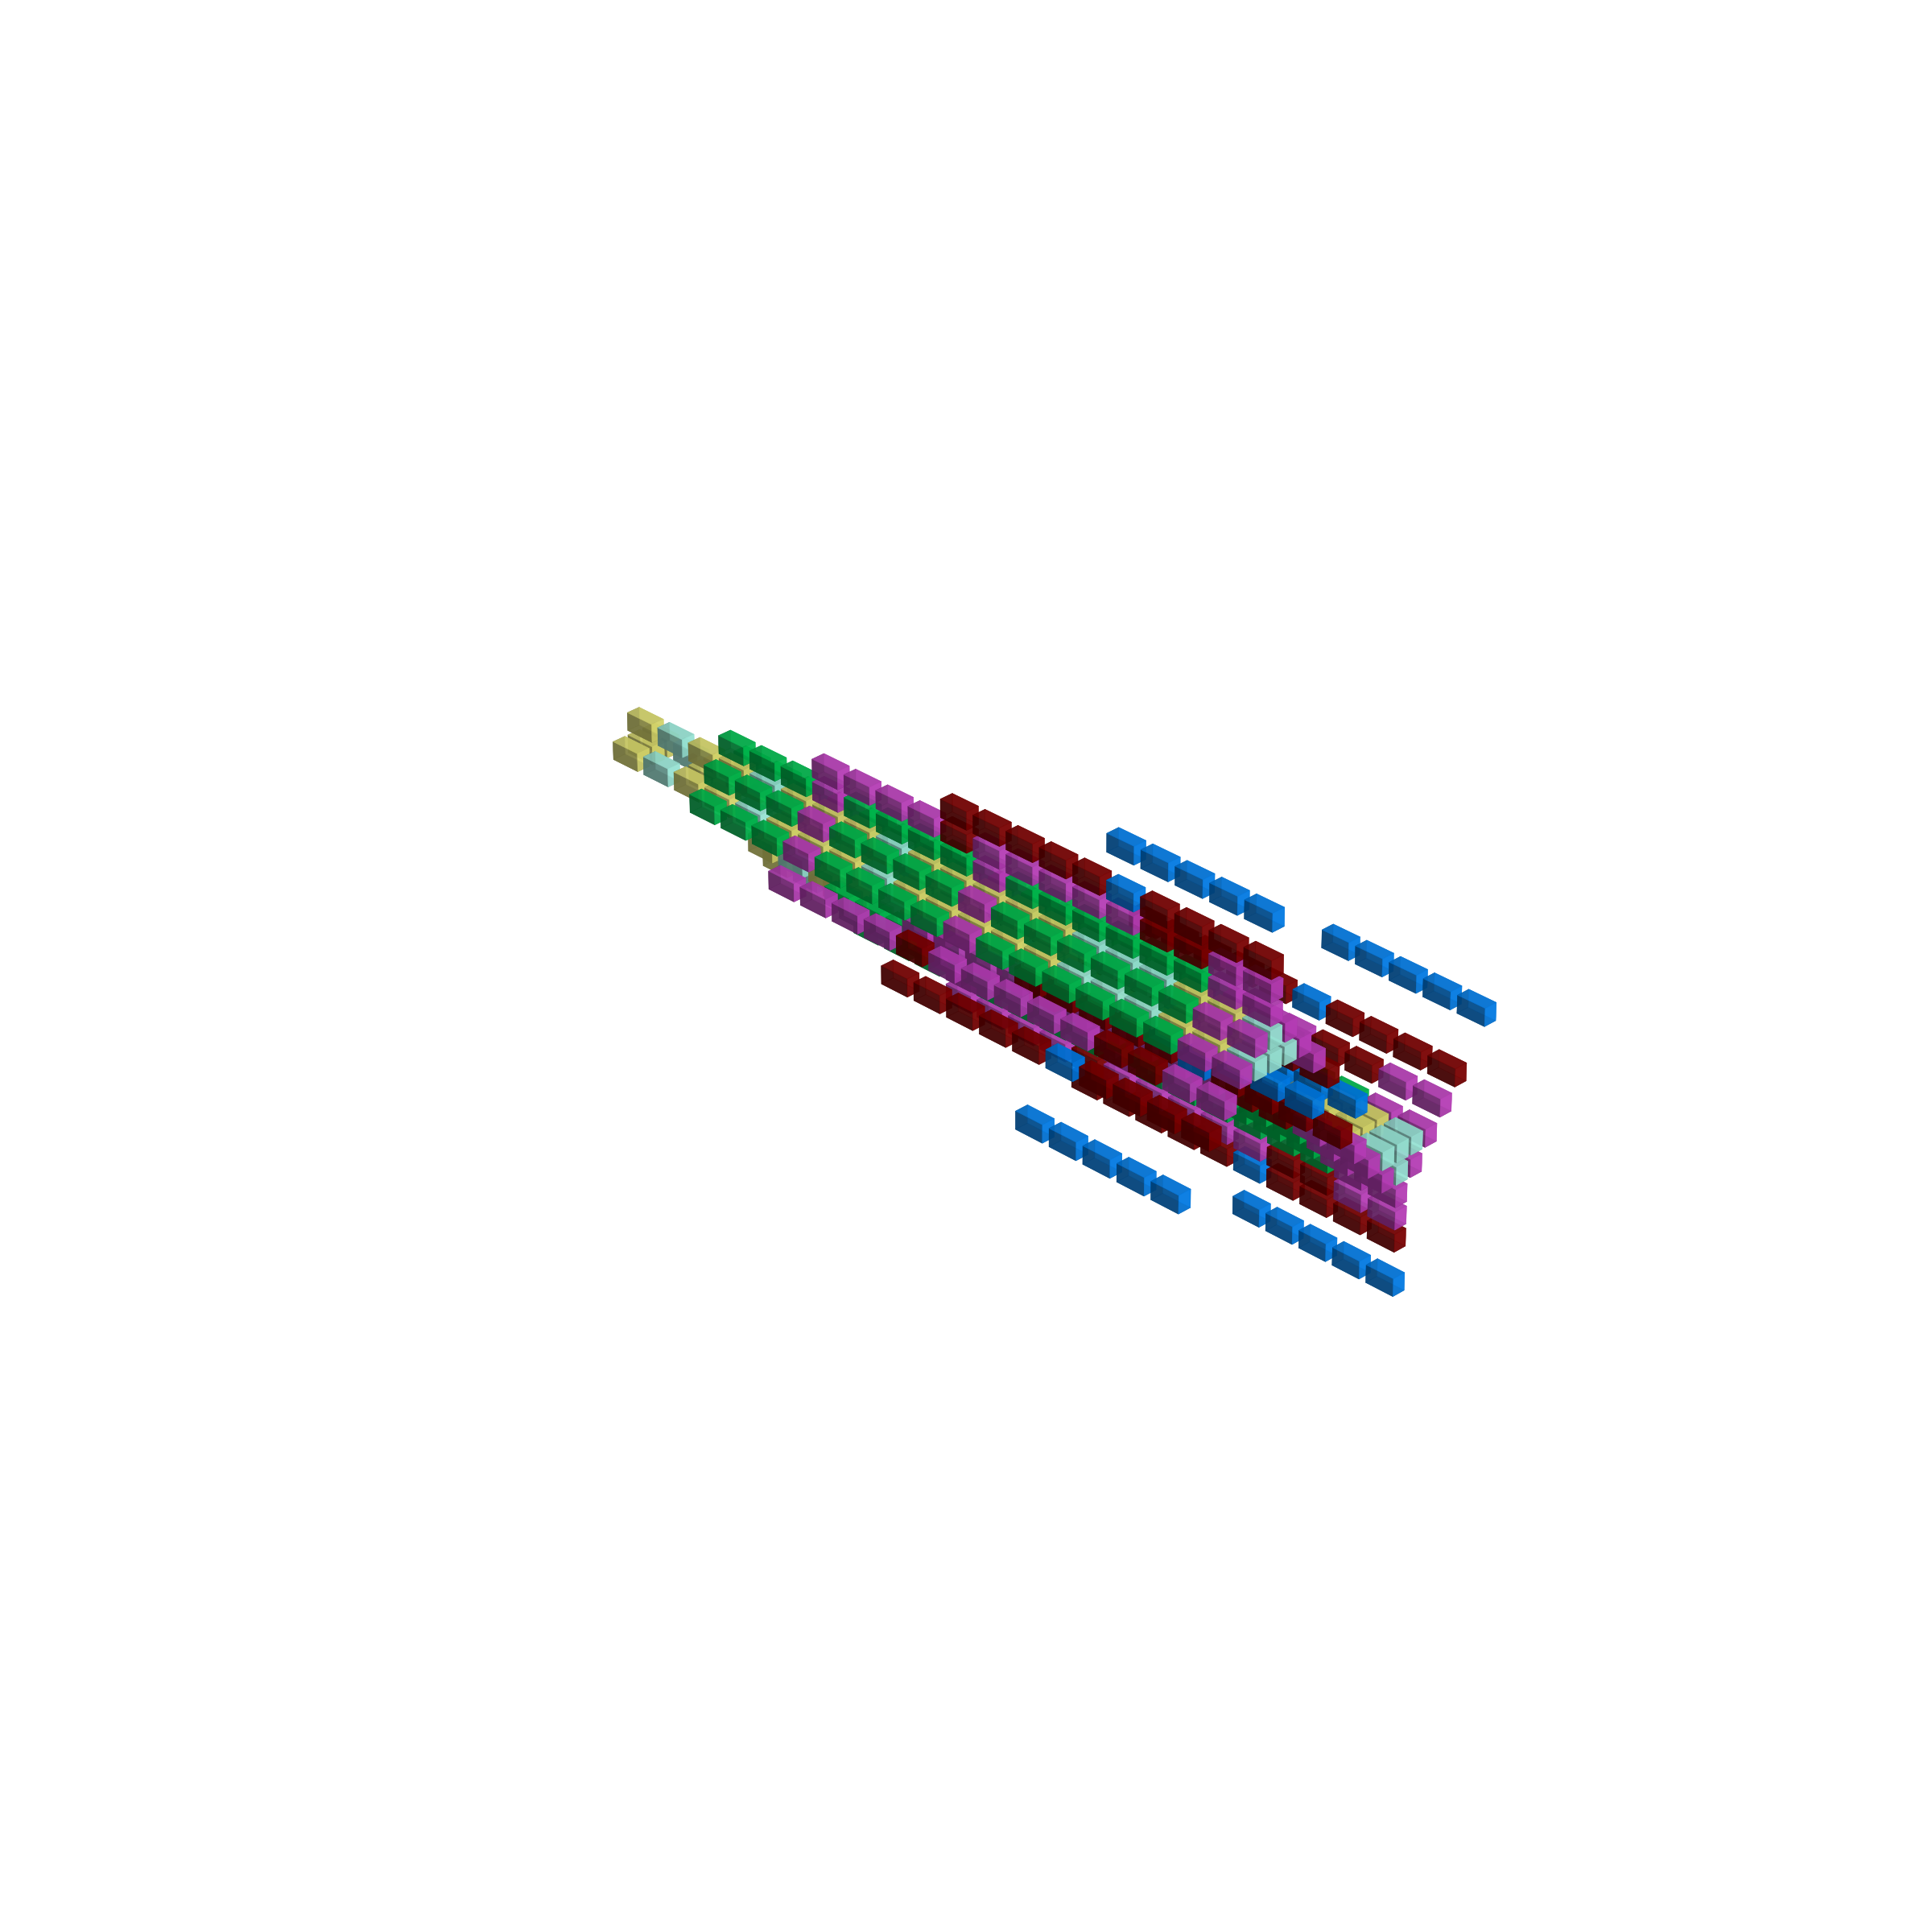
\includegraphics[width=8cm]{src/symmetries/pattern4_2-45.png}\\
        \vspace*{-5cm}
        \hspace*{-3cm}
        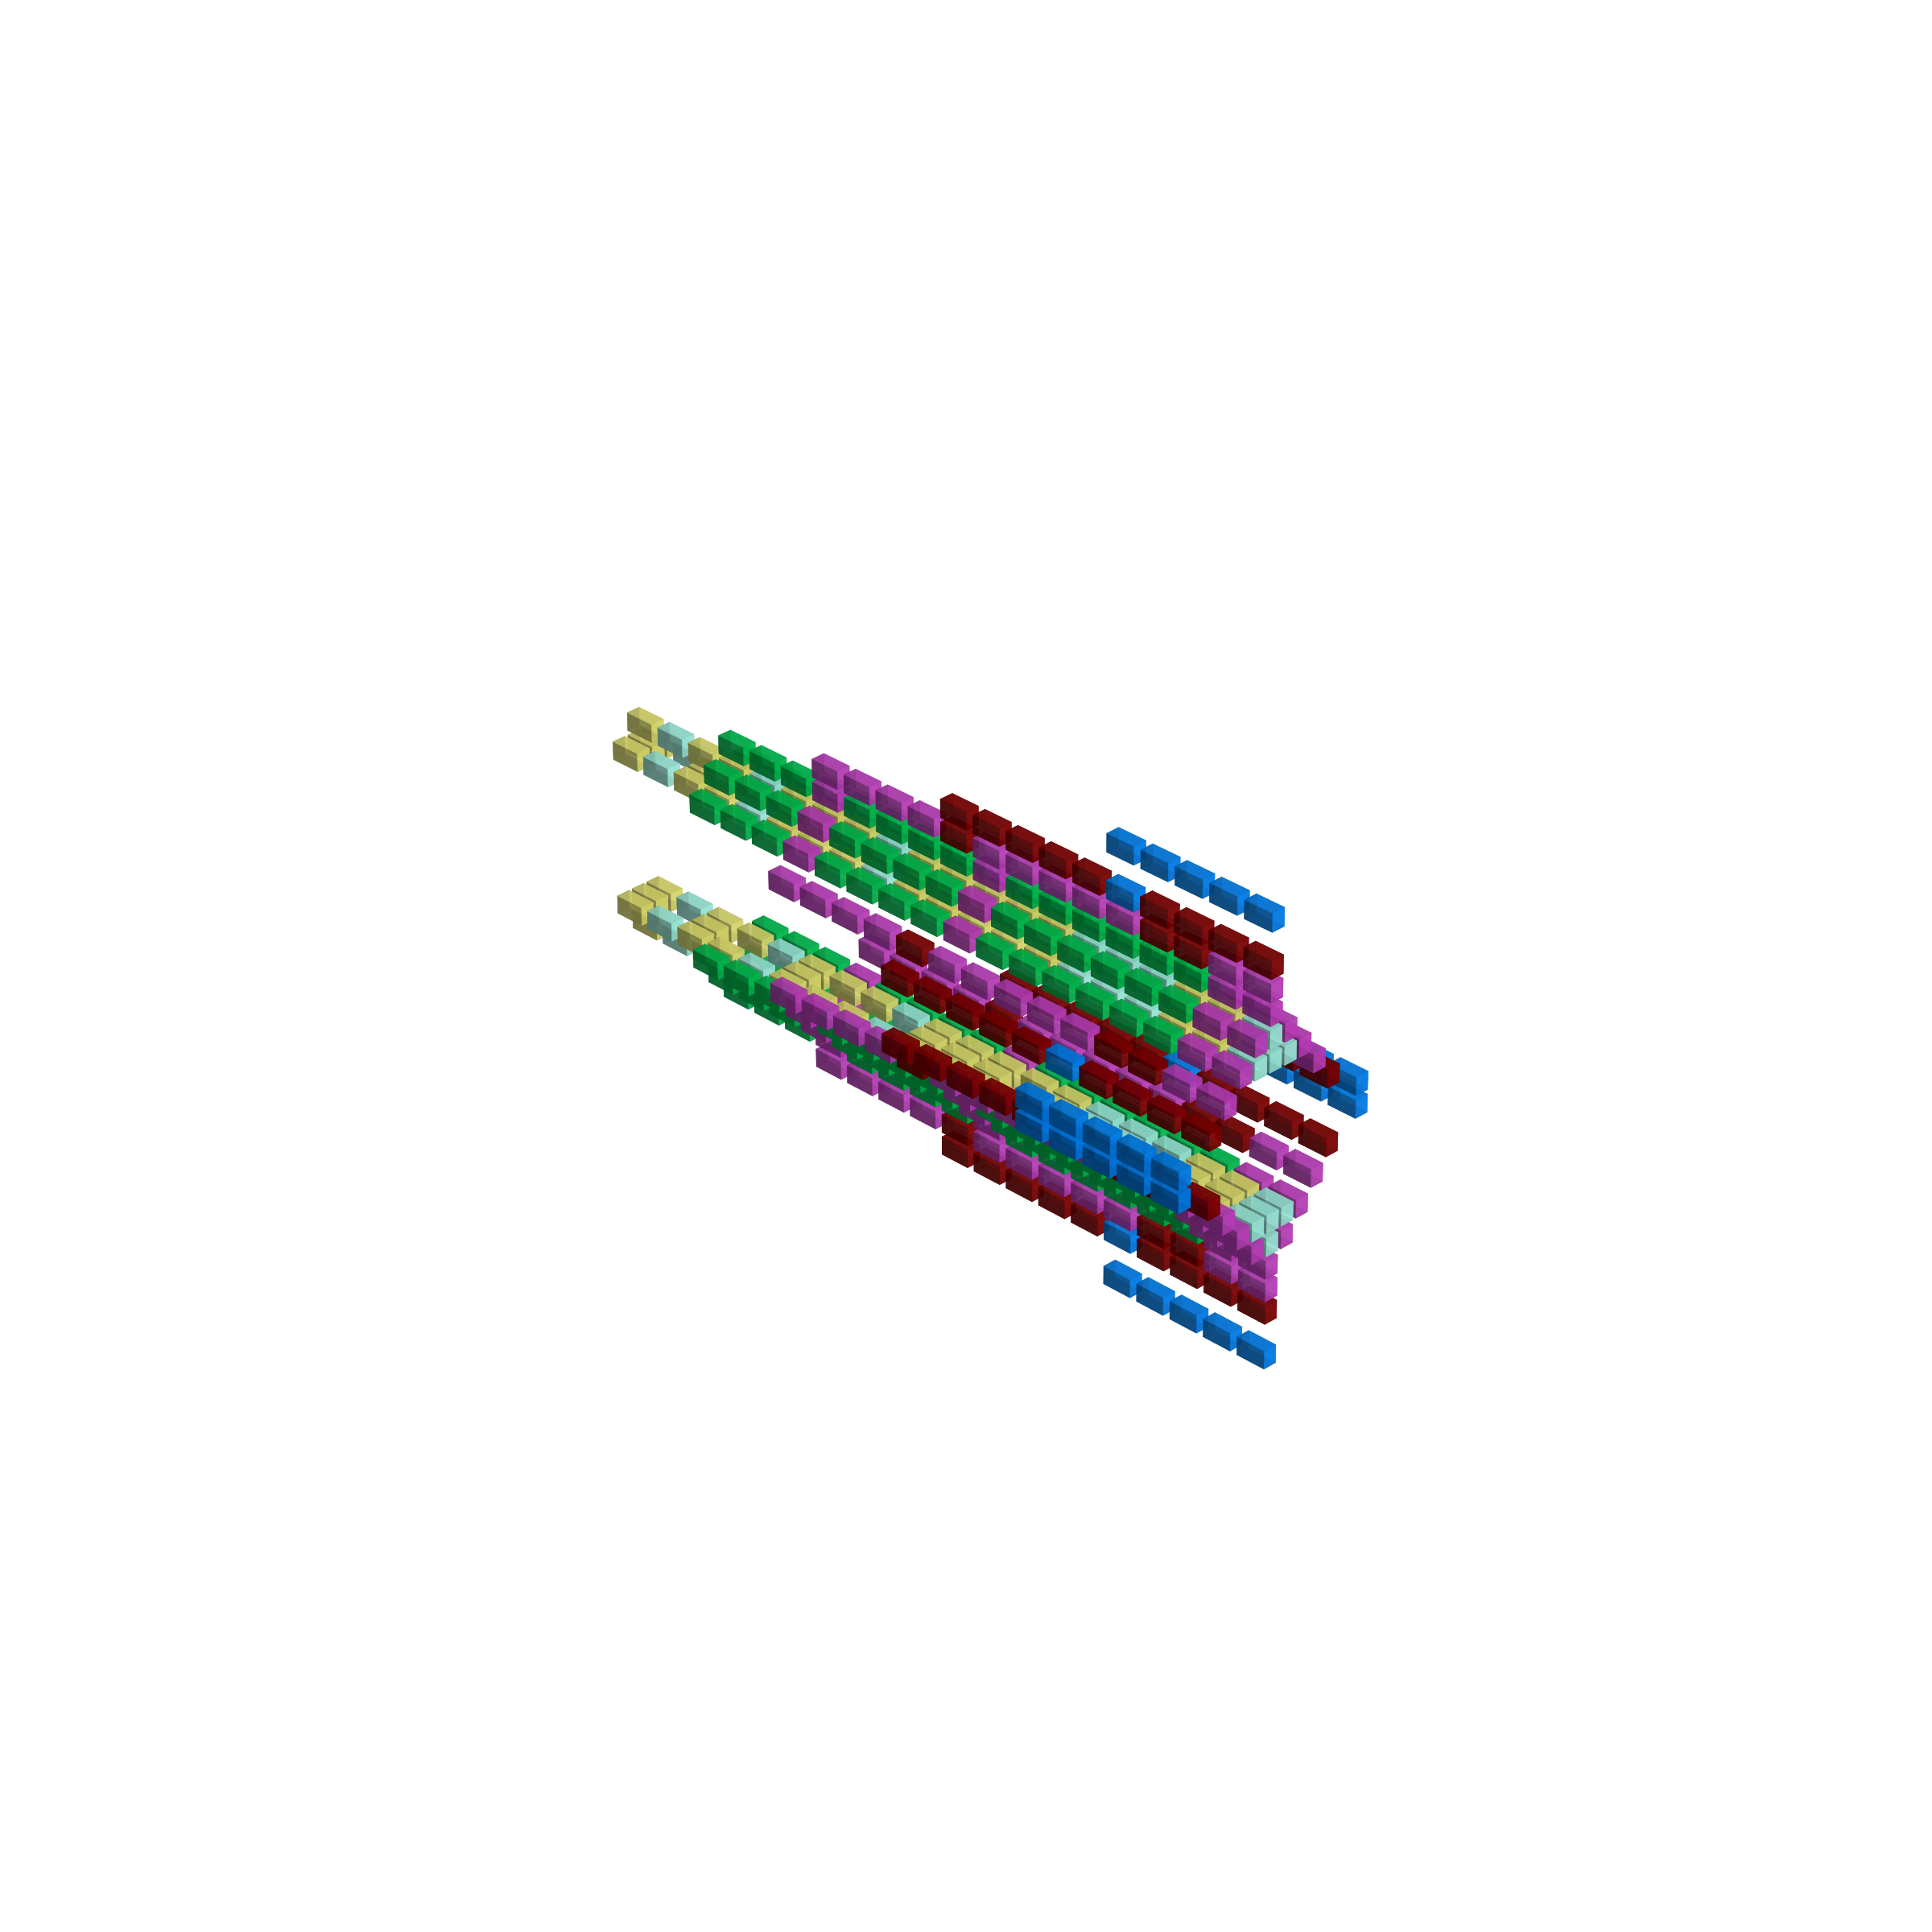
\includegraphics[width=8cm]{src/symmetries/pattern4_3-45.png}\\
        \vspace*{-8cm}
        \hspace*{2cm}
        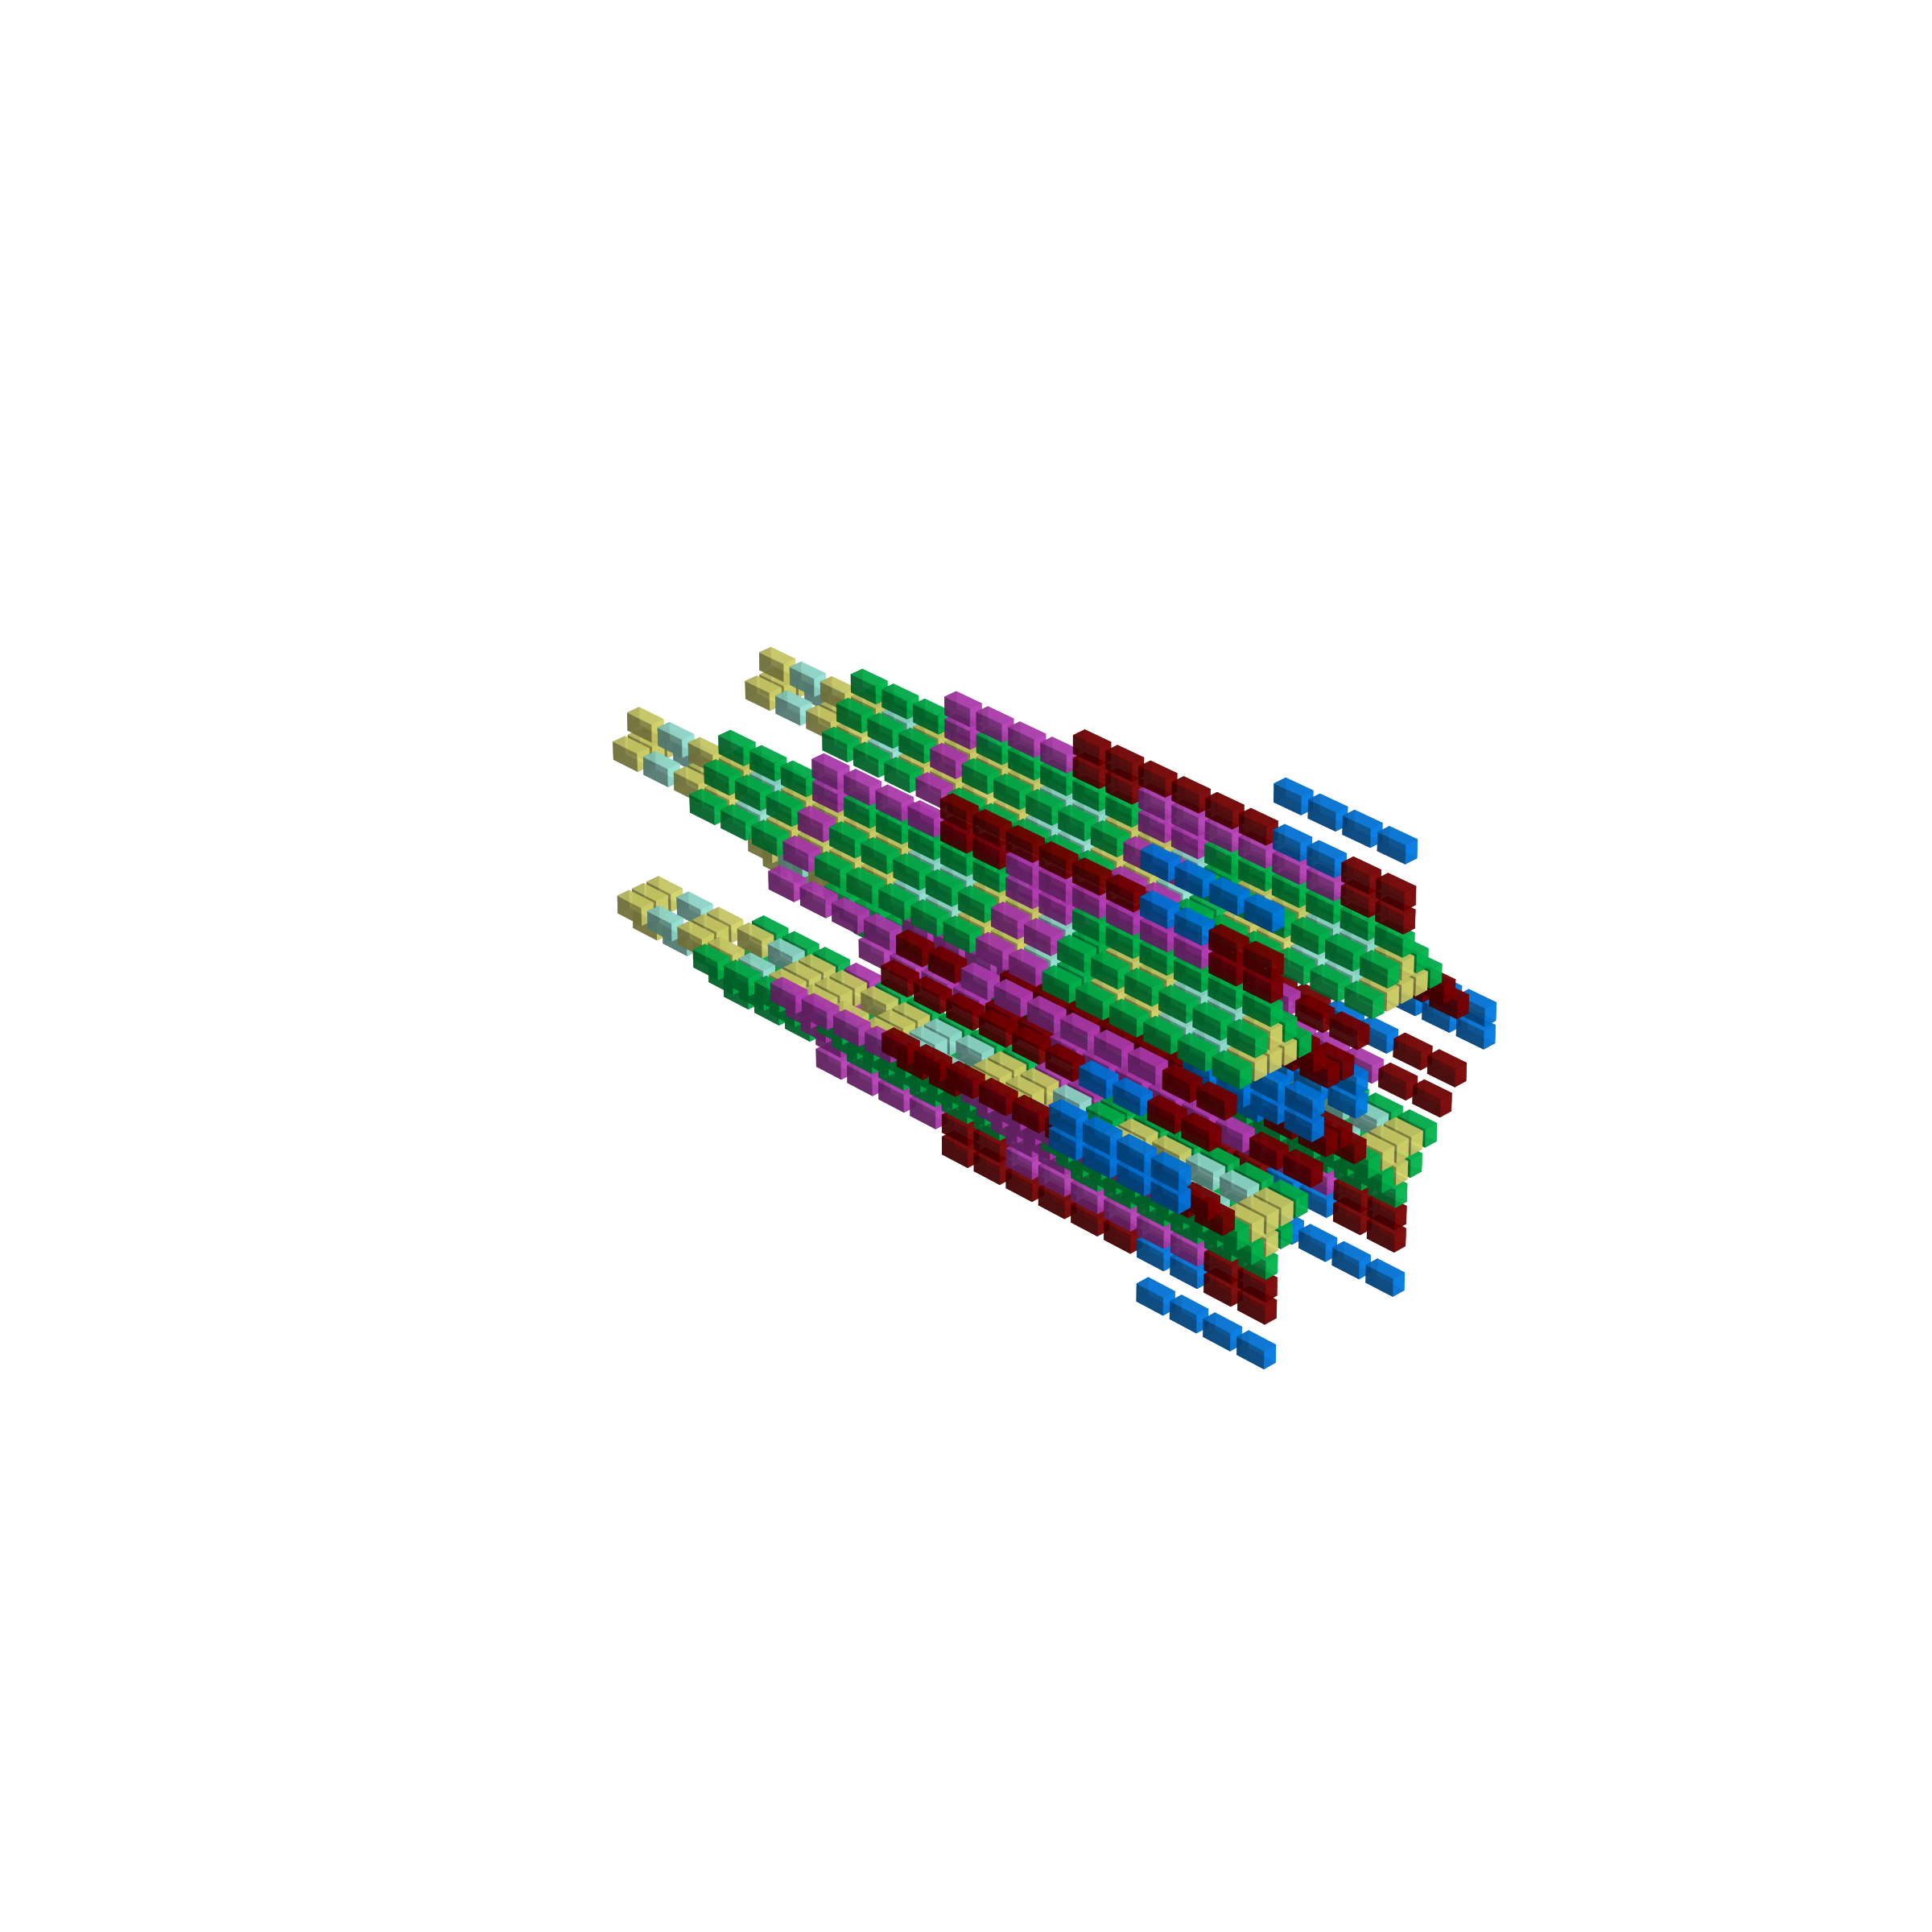
\includegraphics[width=8cm]{src/symmetries/pattern4_4-45.png}
        \vspace*{-2.5cm}
  \caption*{\getItem{4}}
  \end{figure}
\end{minipage}
\hspace{1cm}
\begin{minipage}[b]{0.50\linewidth}                                       
  \begin{figure}[H]
      \centering
        \vspace*{-1cm}
        \hspace*{-2cm}
        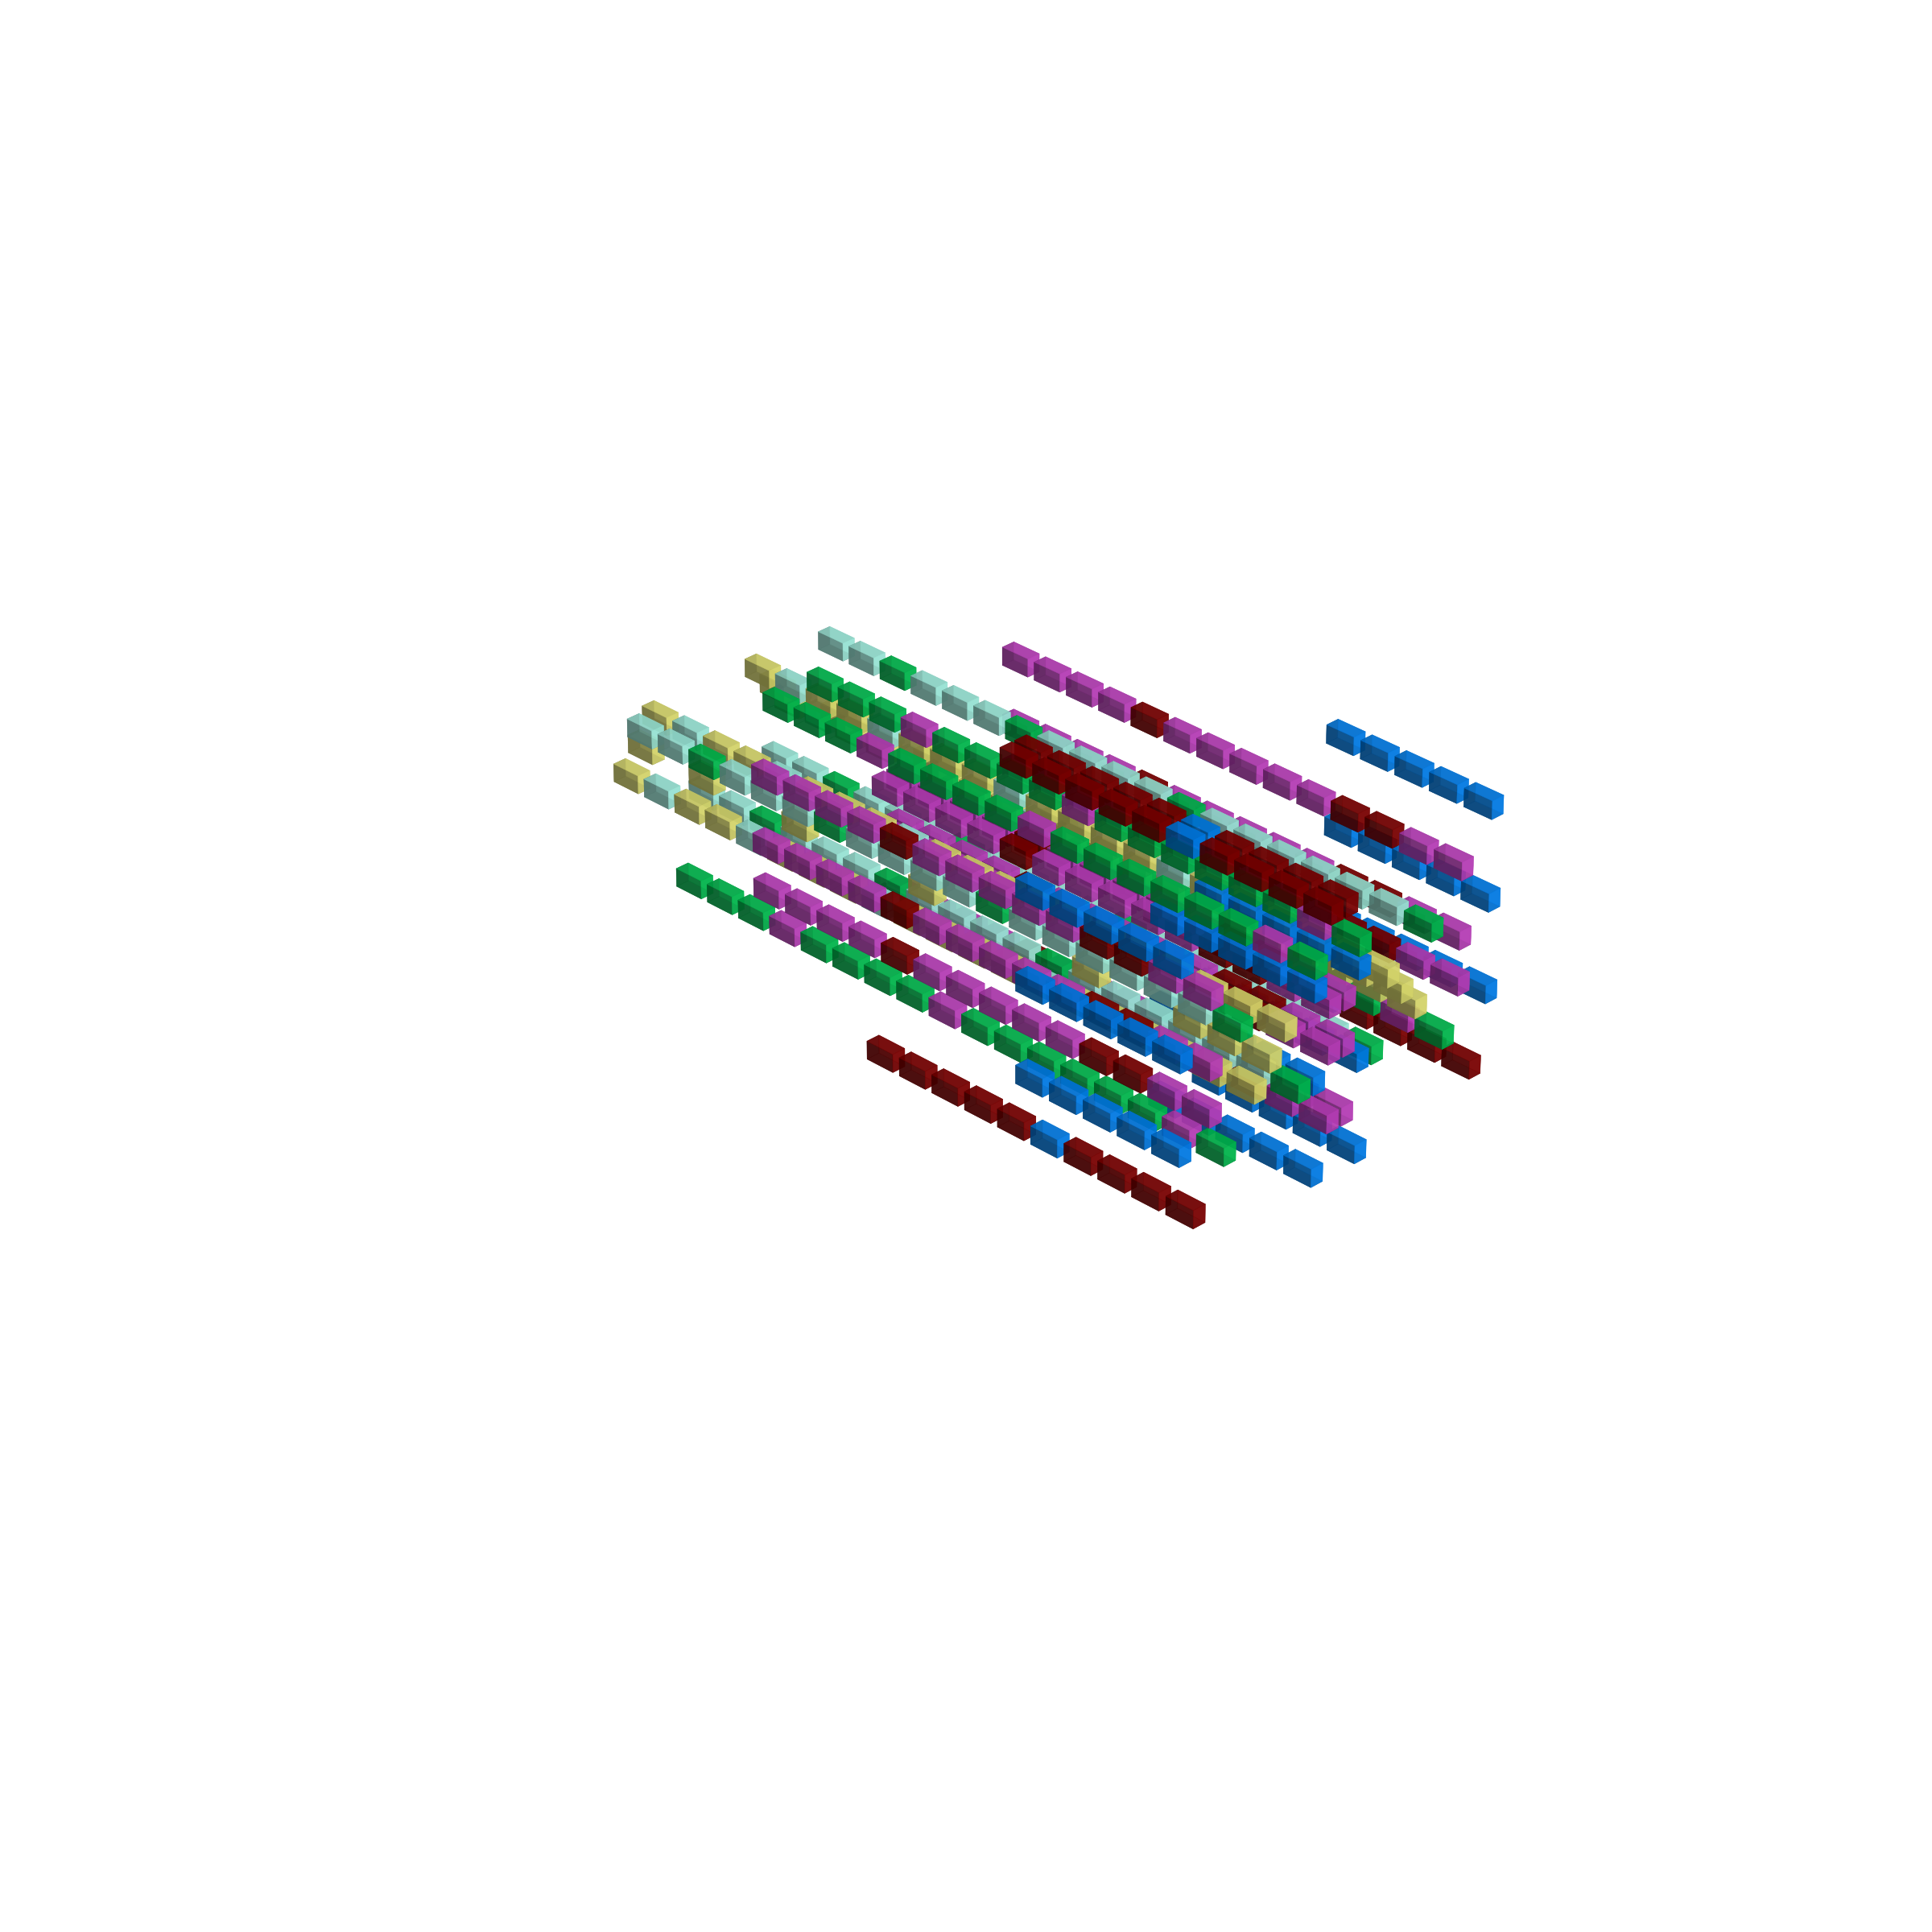
\includegraphics[width=8cm]{src/symmetries/pattern5_1-45.png}%
        \hspace*{-4cm}
        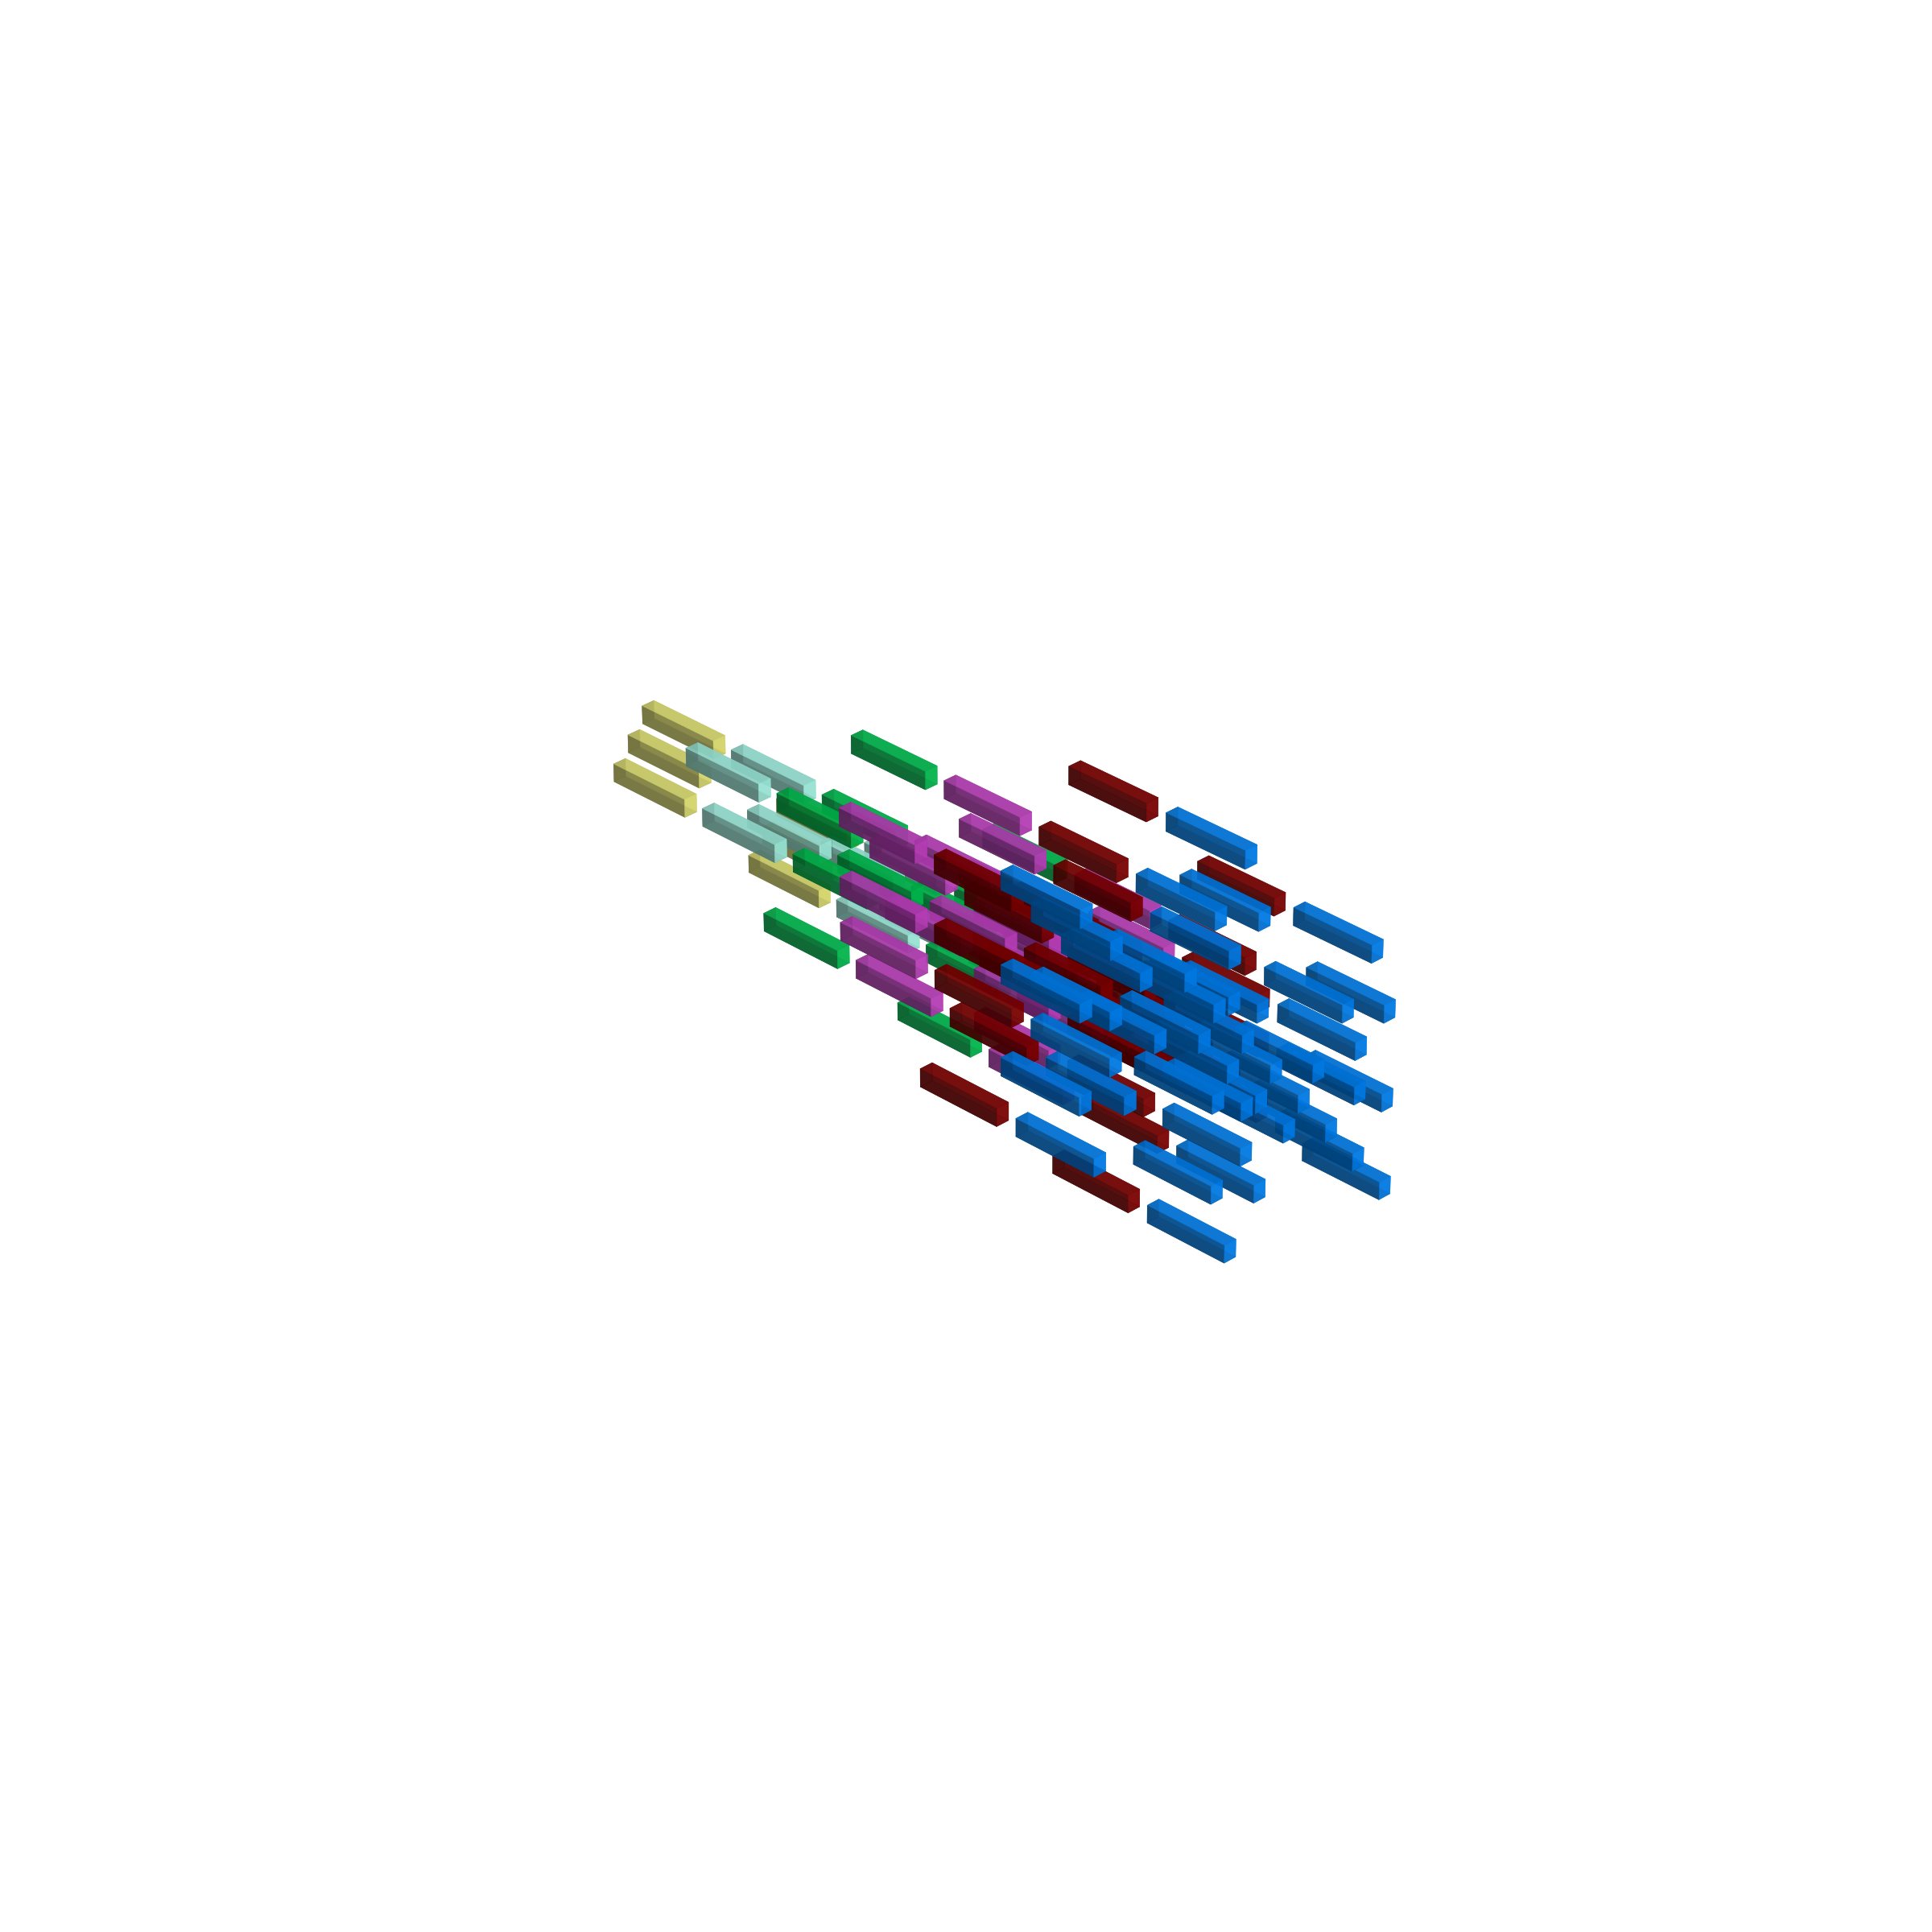
\includegraphics[width=8cm]{src/symmetries/pattern5_2-45.png}\\
        \vspace*{-5cm}
        \hspace*{-1cm}
        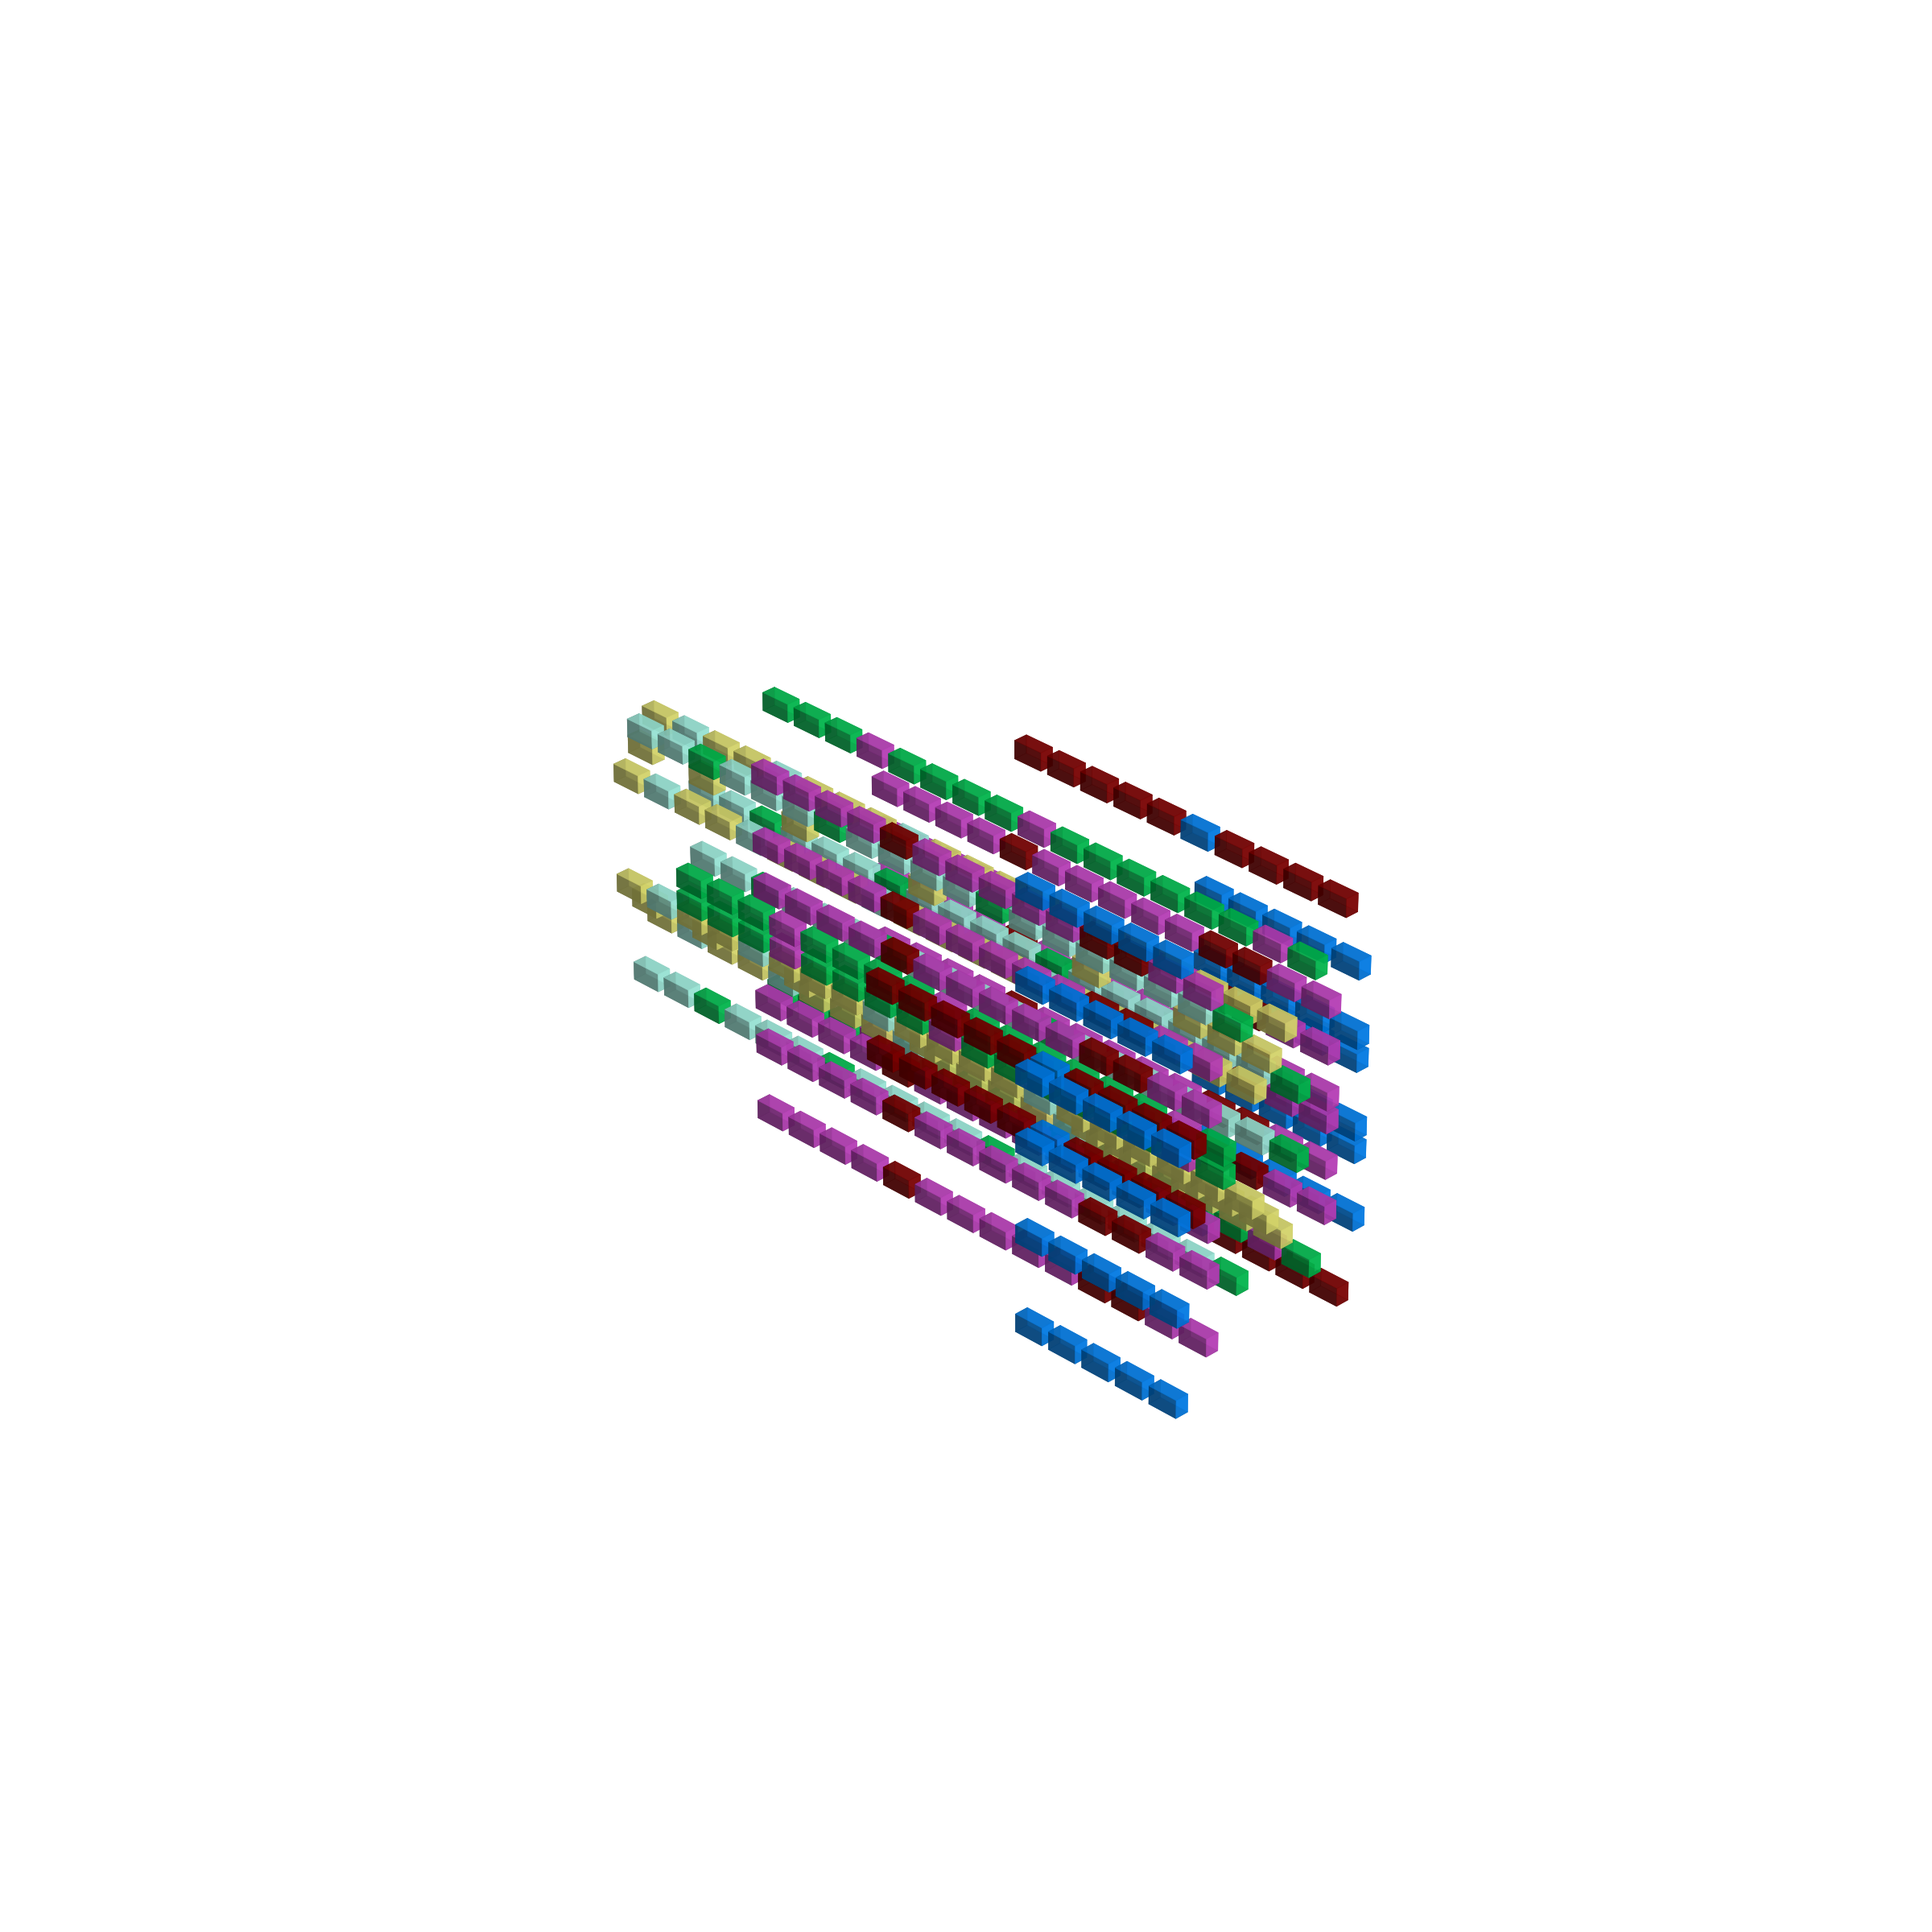
\includegraphics[width=8cm]{src/symmetries/pattern5_3-45.png}\\
        \vspace*{-8cm}
        \hspace*{2cm}
        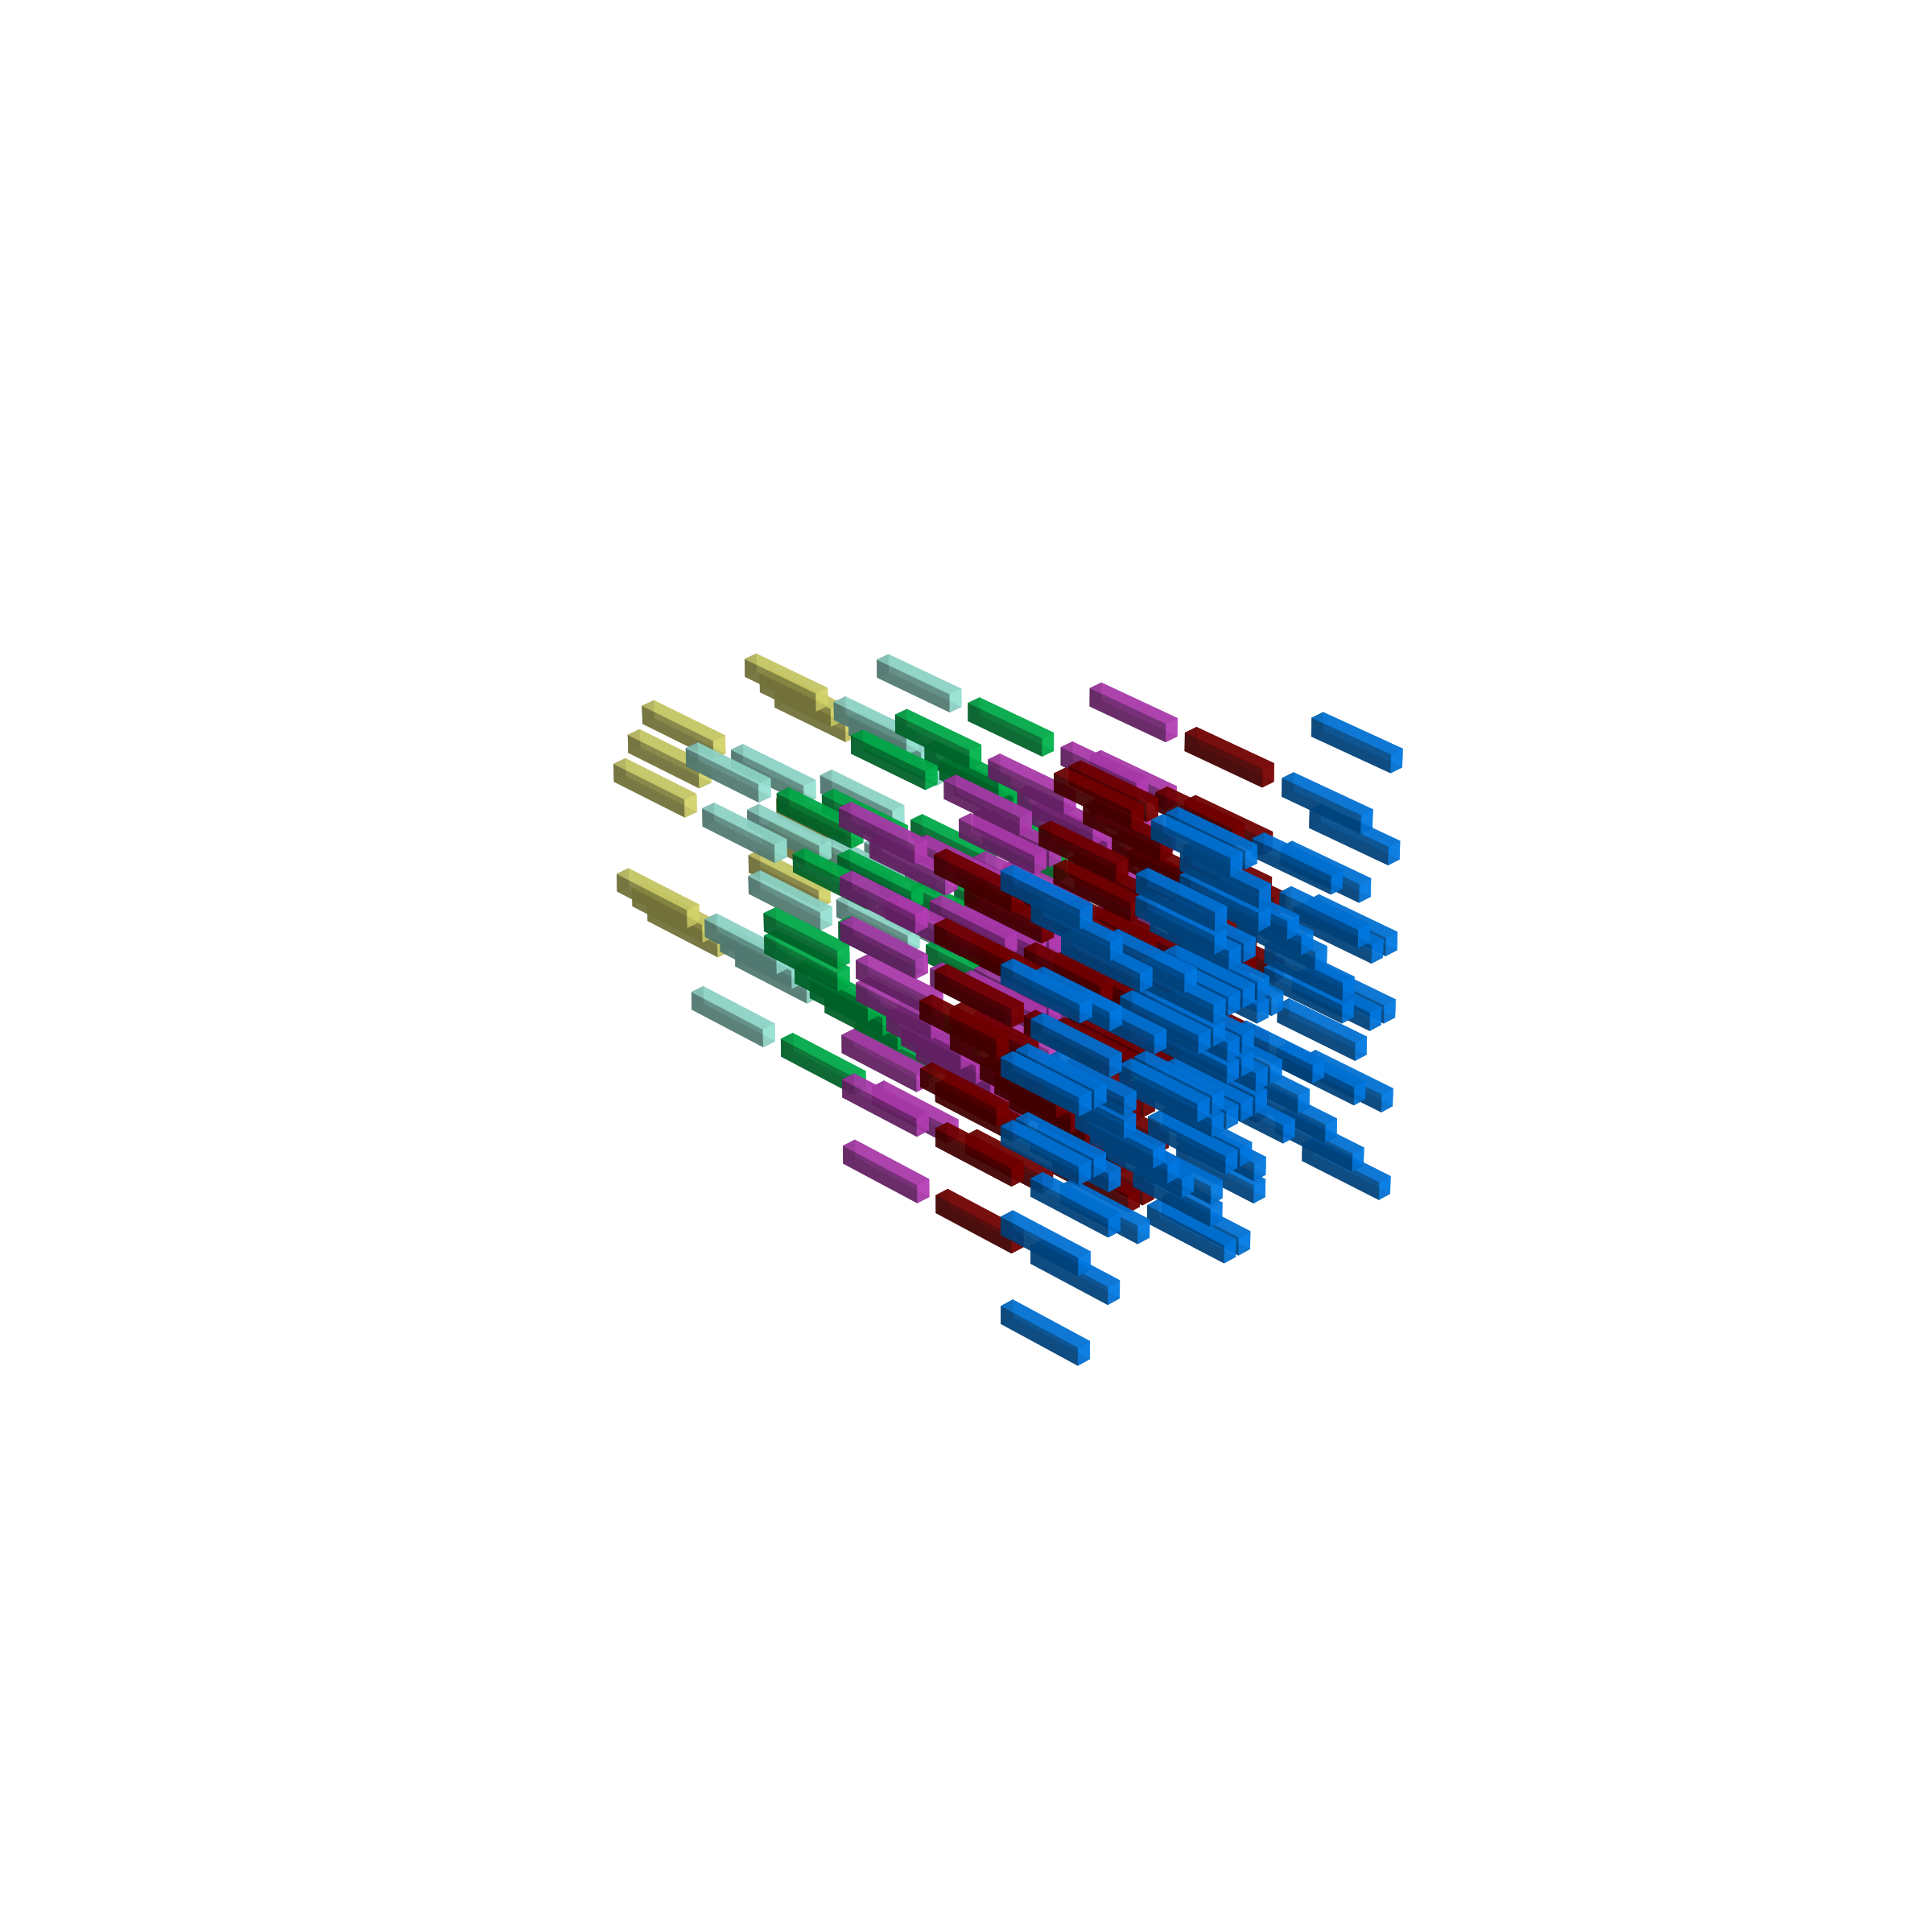
\includegraphics[width=8cm]{src/symmetries/pattern5_4-45.png}
        \vspace*{-2.5cm}
  \caption*{\getItem{5}}
  \end{figure}
\end{minipage}
\clearpage
\hspace{-1cm}
\begin{minipage}[b]{0.50\linewidth}                                       
  \begin{figure}[H]
      \centering
        \vspace*{-1cm}
        \hspace*{-2cm}
        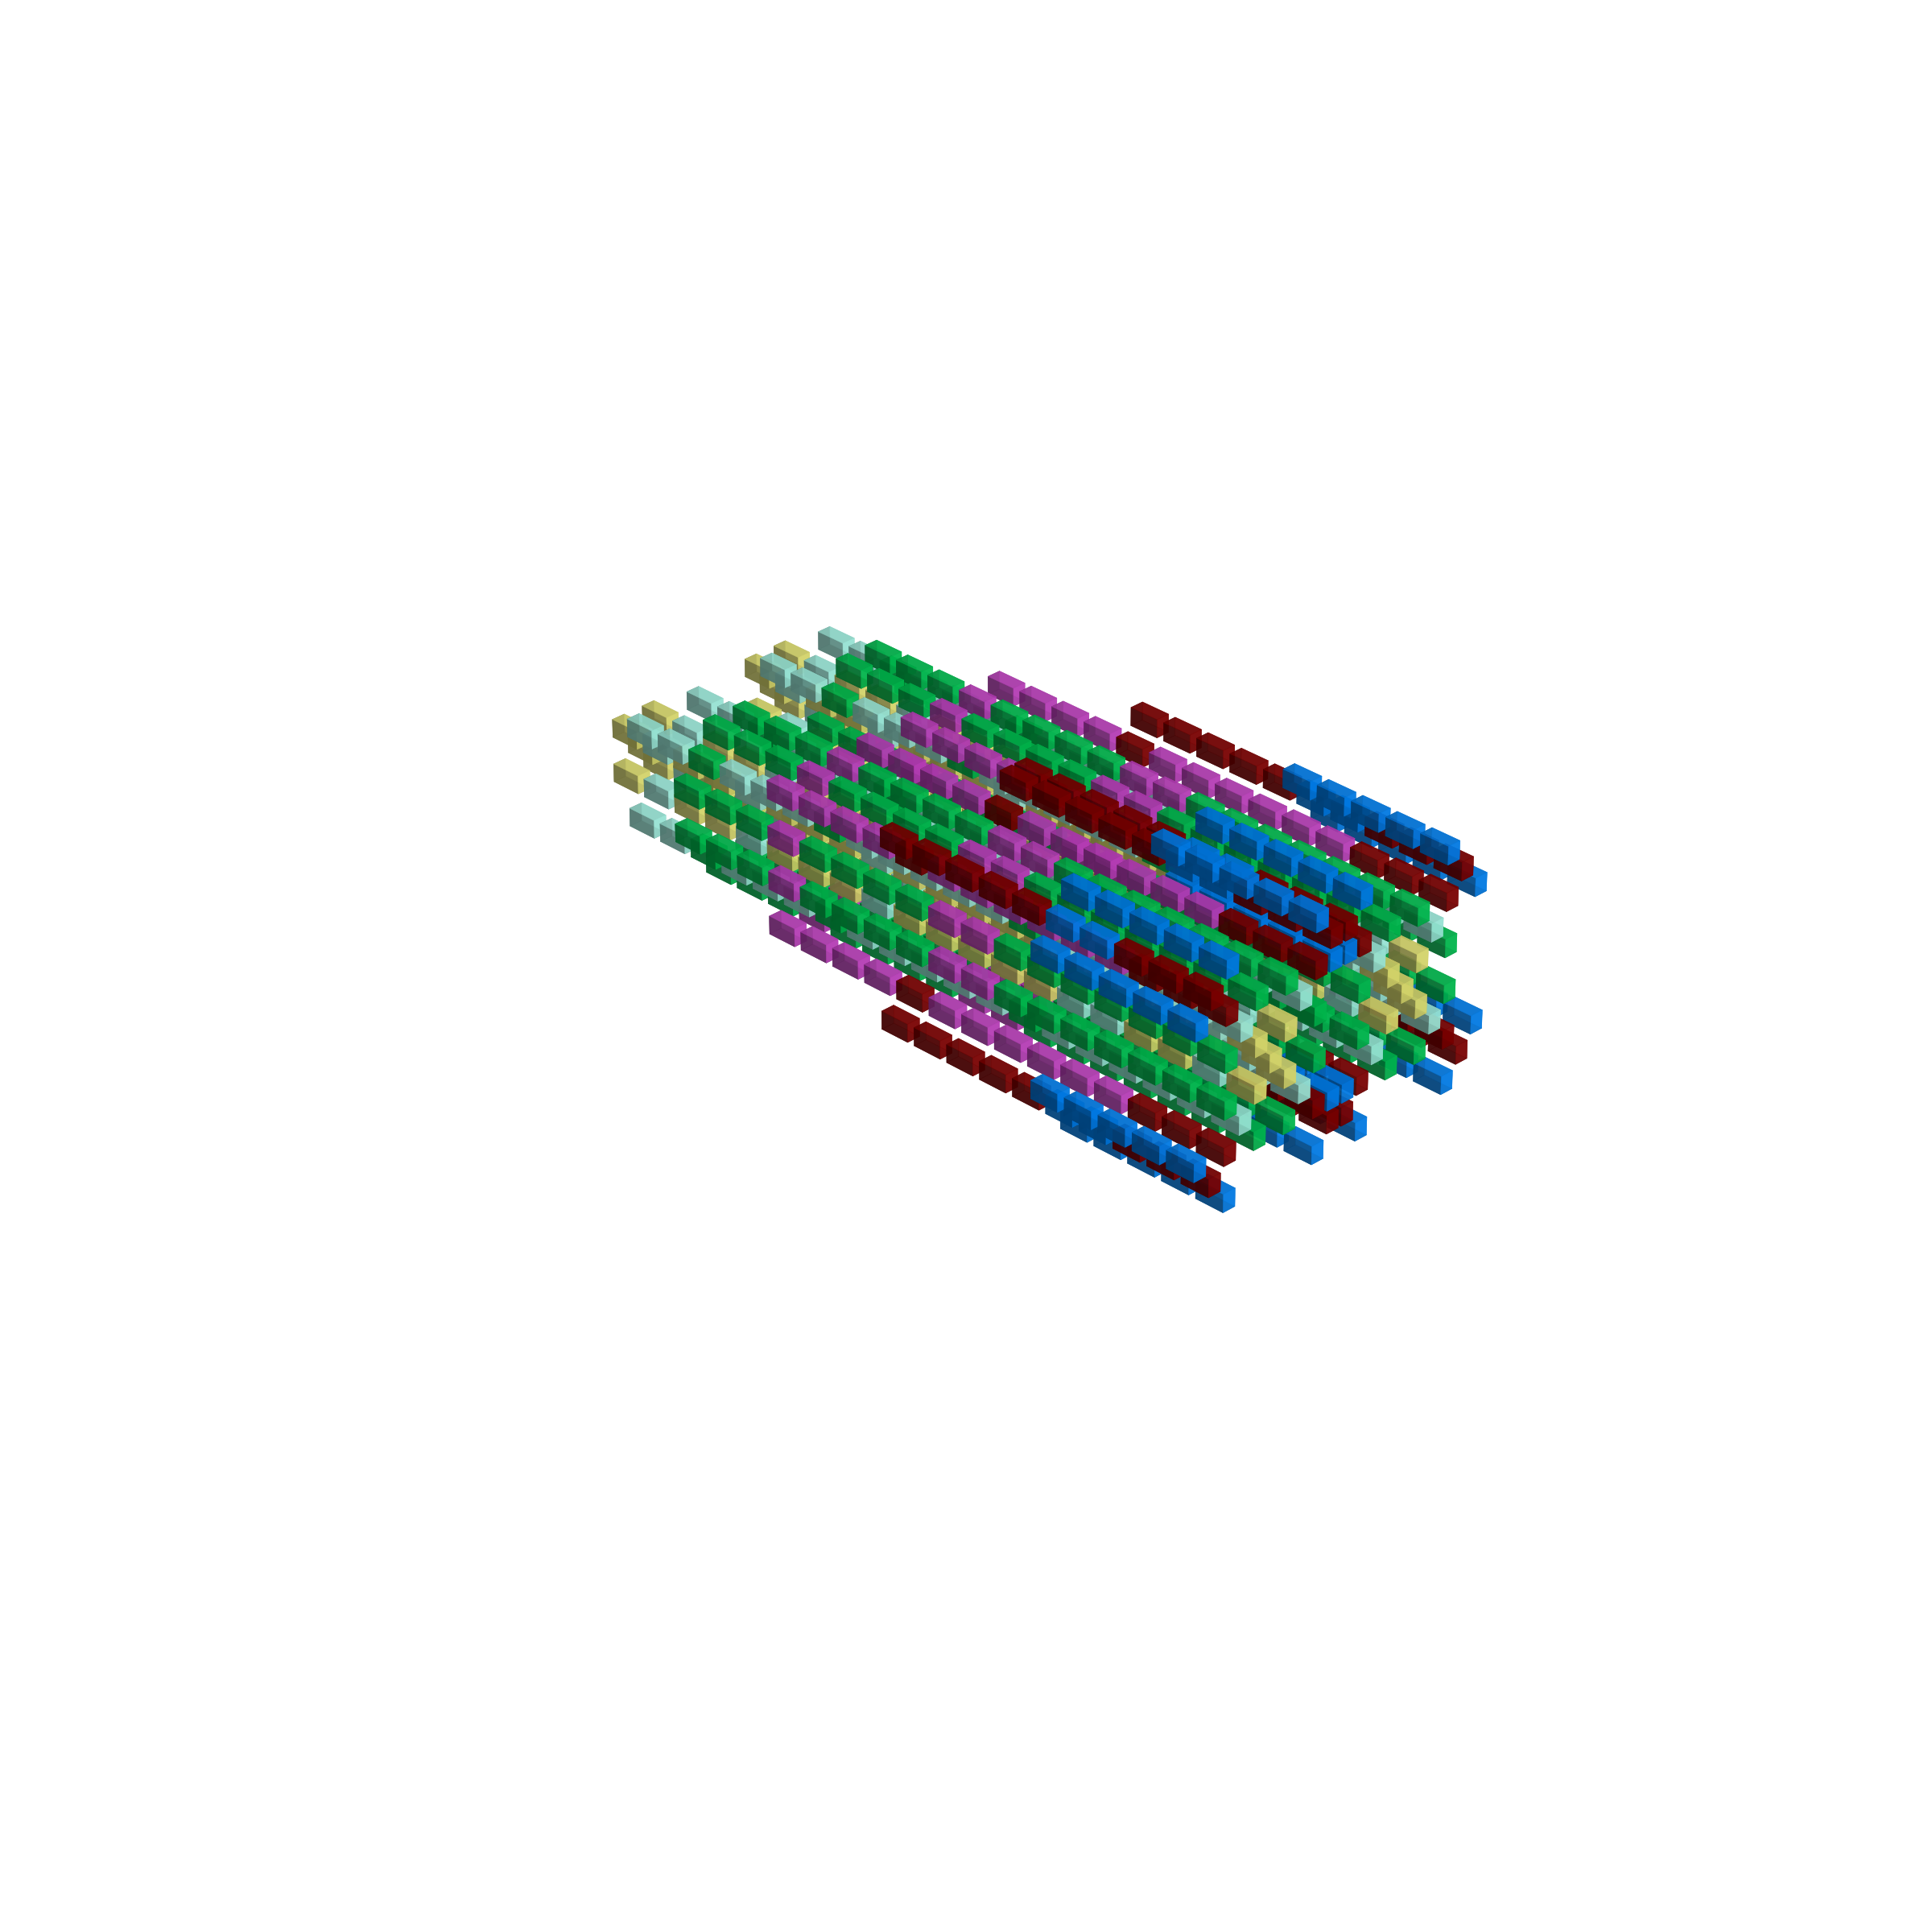
\includegraphics[width=8cm]{src/symmetries/pattern6_1-45.png}%
        \hspace*{-4cm}
        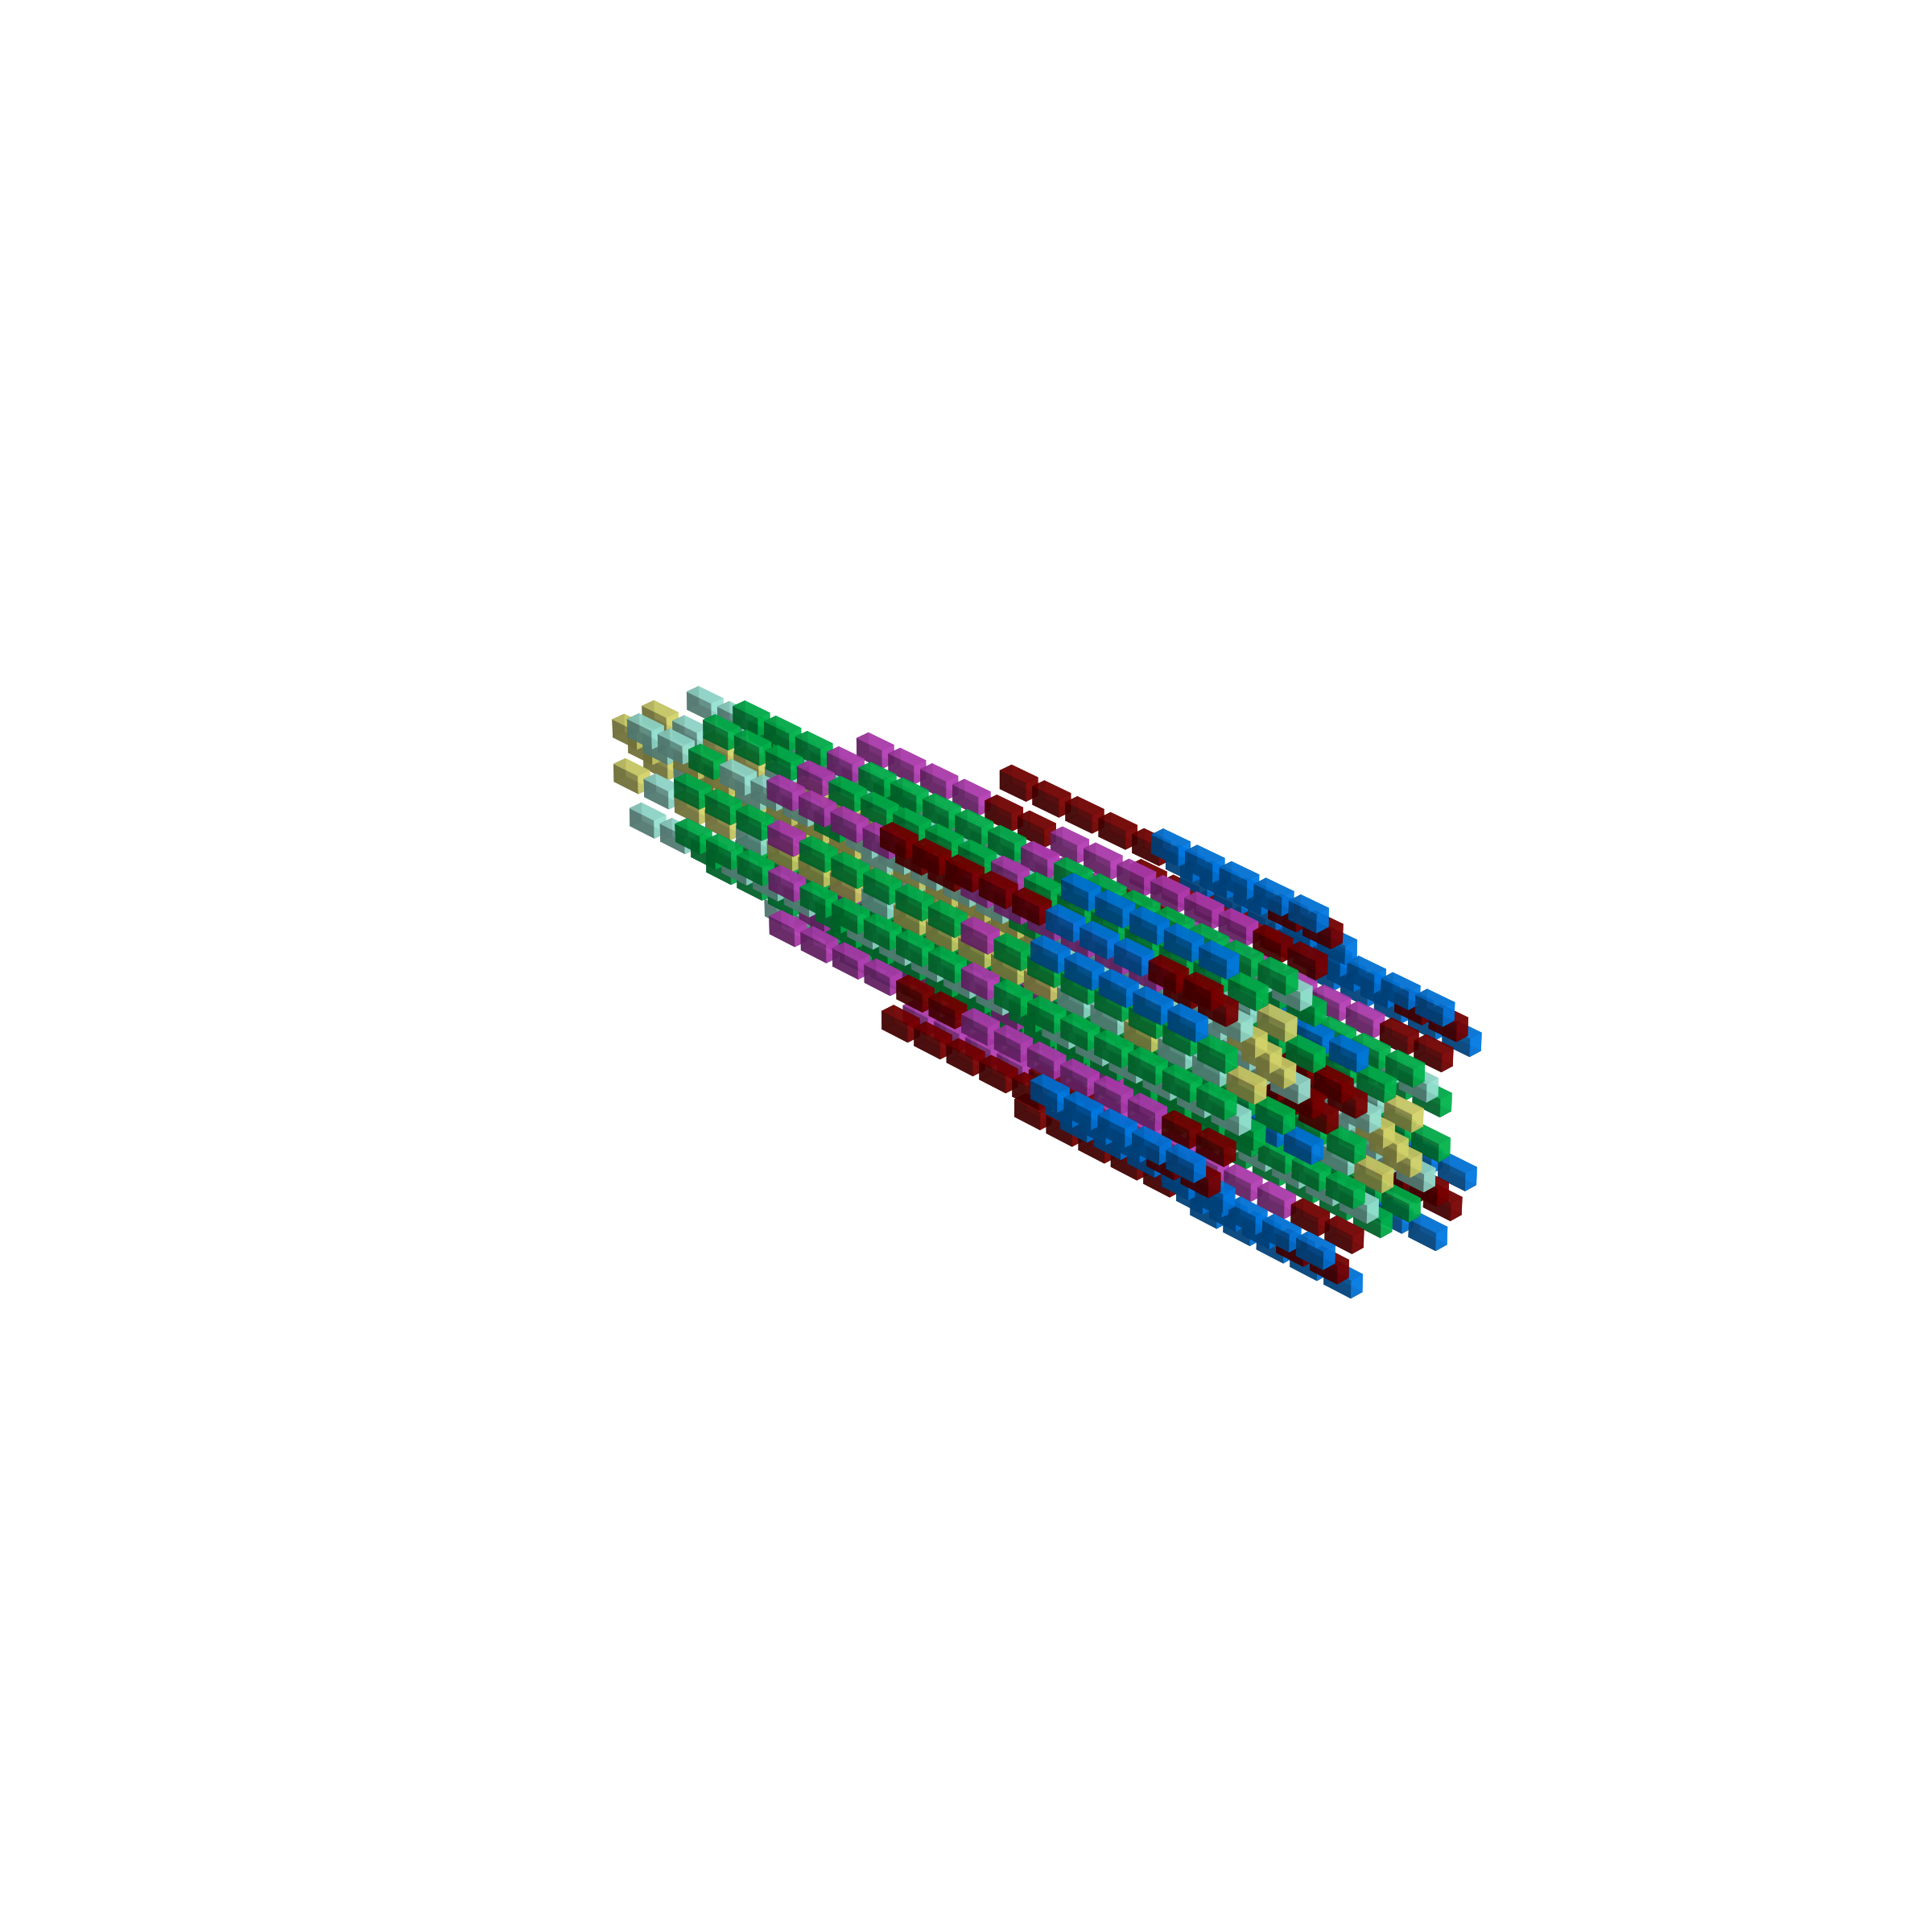
\includegraphics[width=8cm]{src/symmetries/pattern6_2-45.png}\\
        \vspace*{-5cm}
        \hspace*{-3cm}
        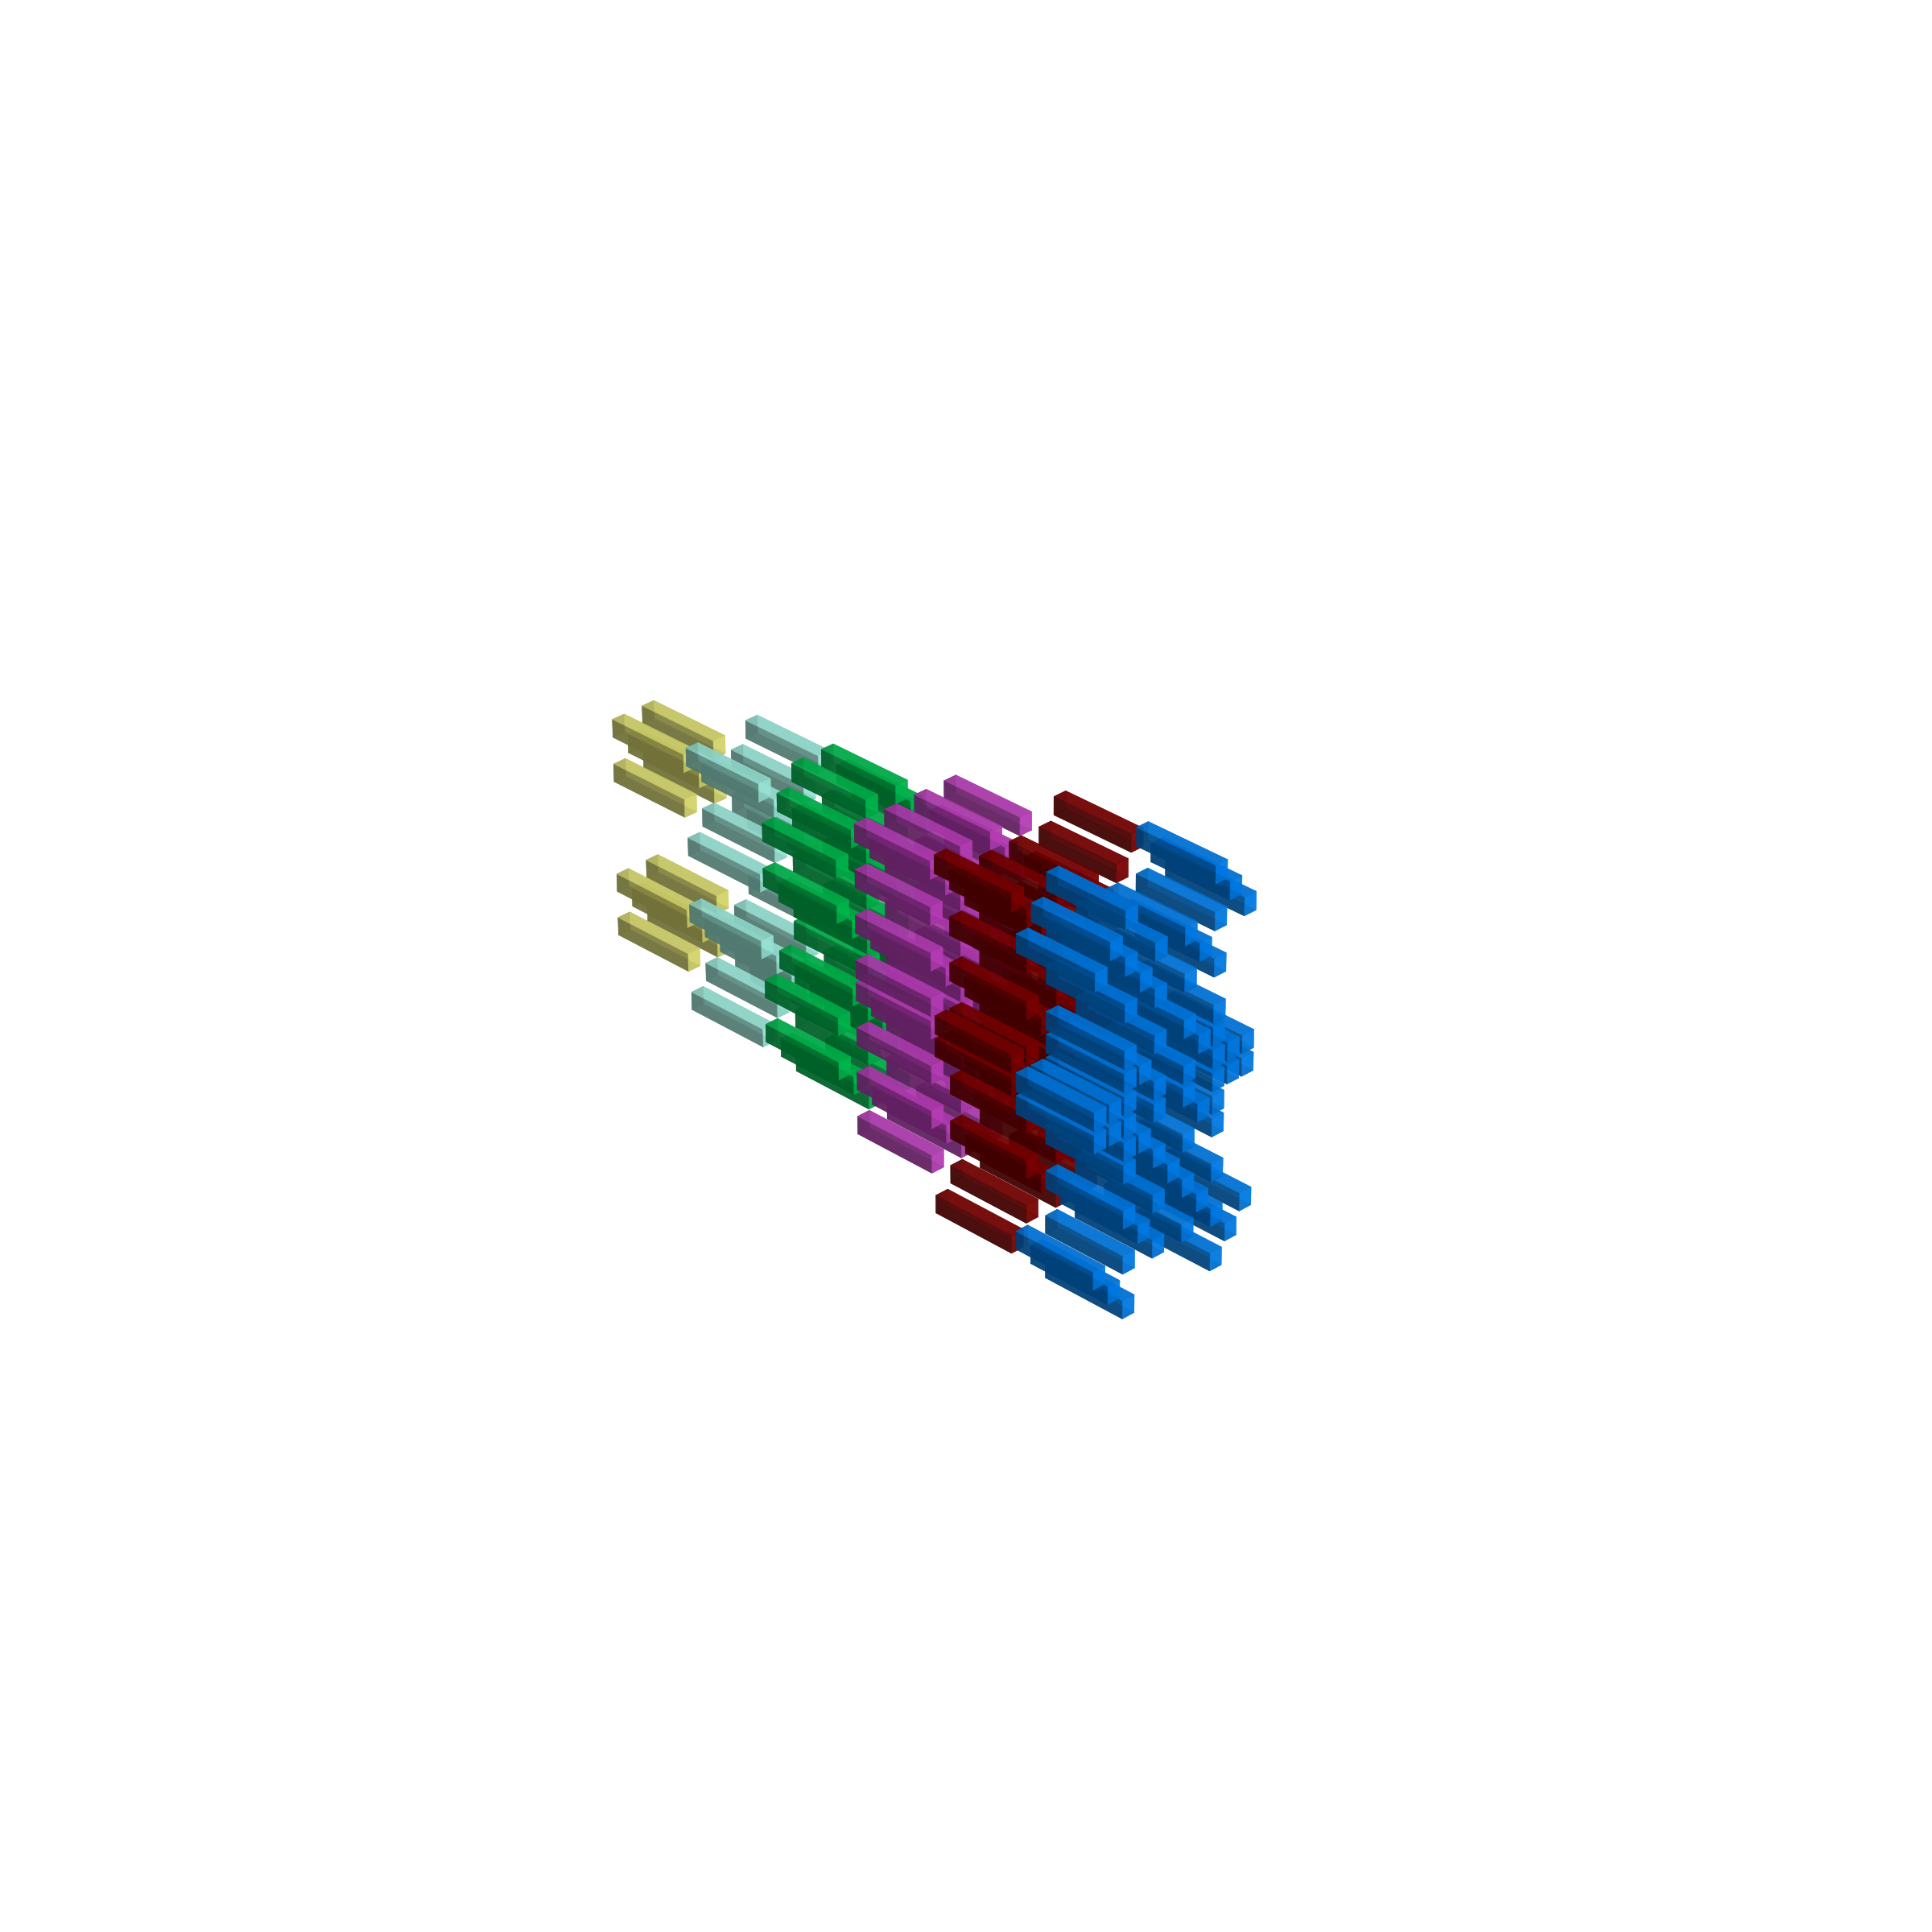
\includegraphics[width=8cm]{src/symmetries/pattern6_3-45.png}\\
        \vspace*{-8cm}
        \hspace*{2cm}
        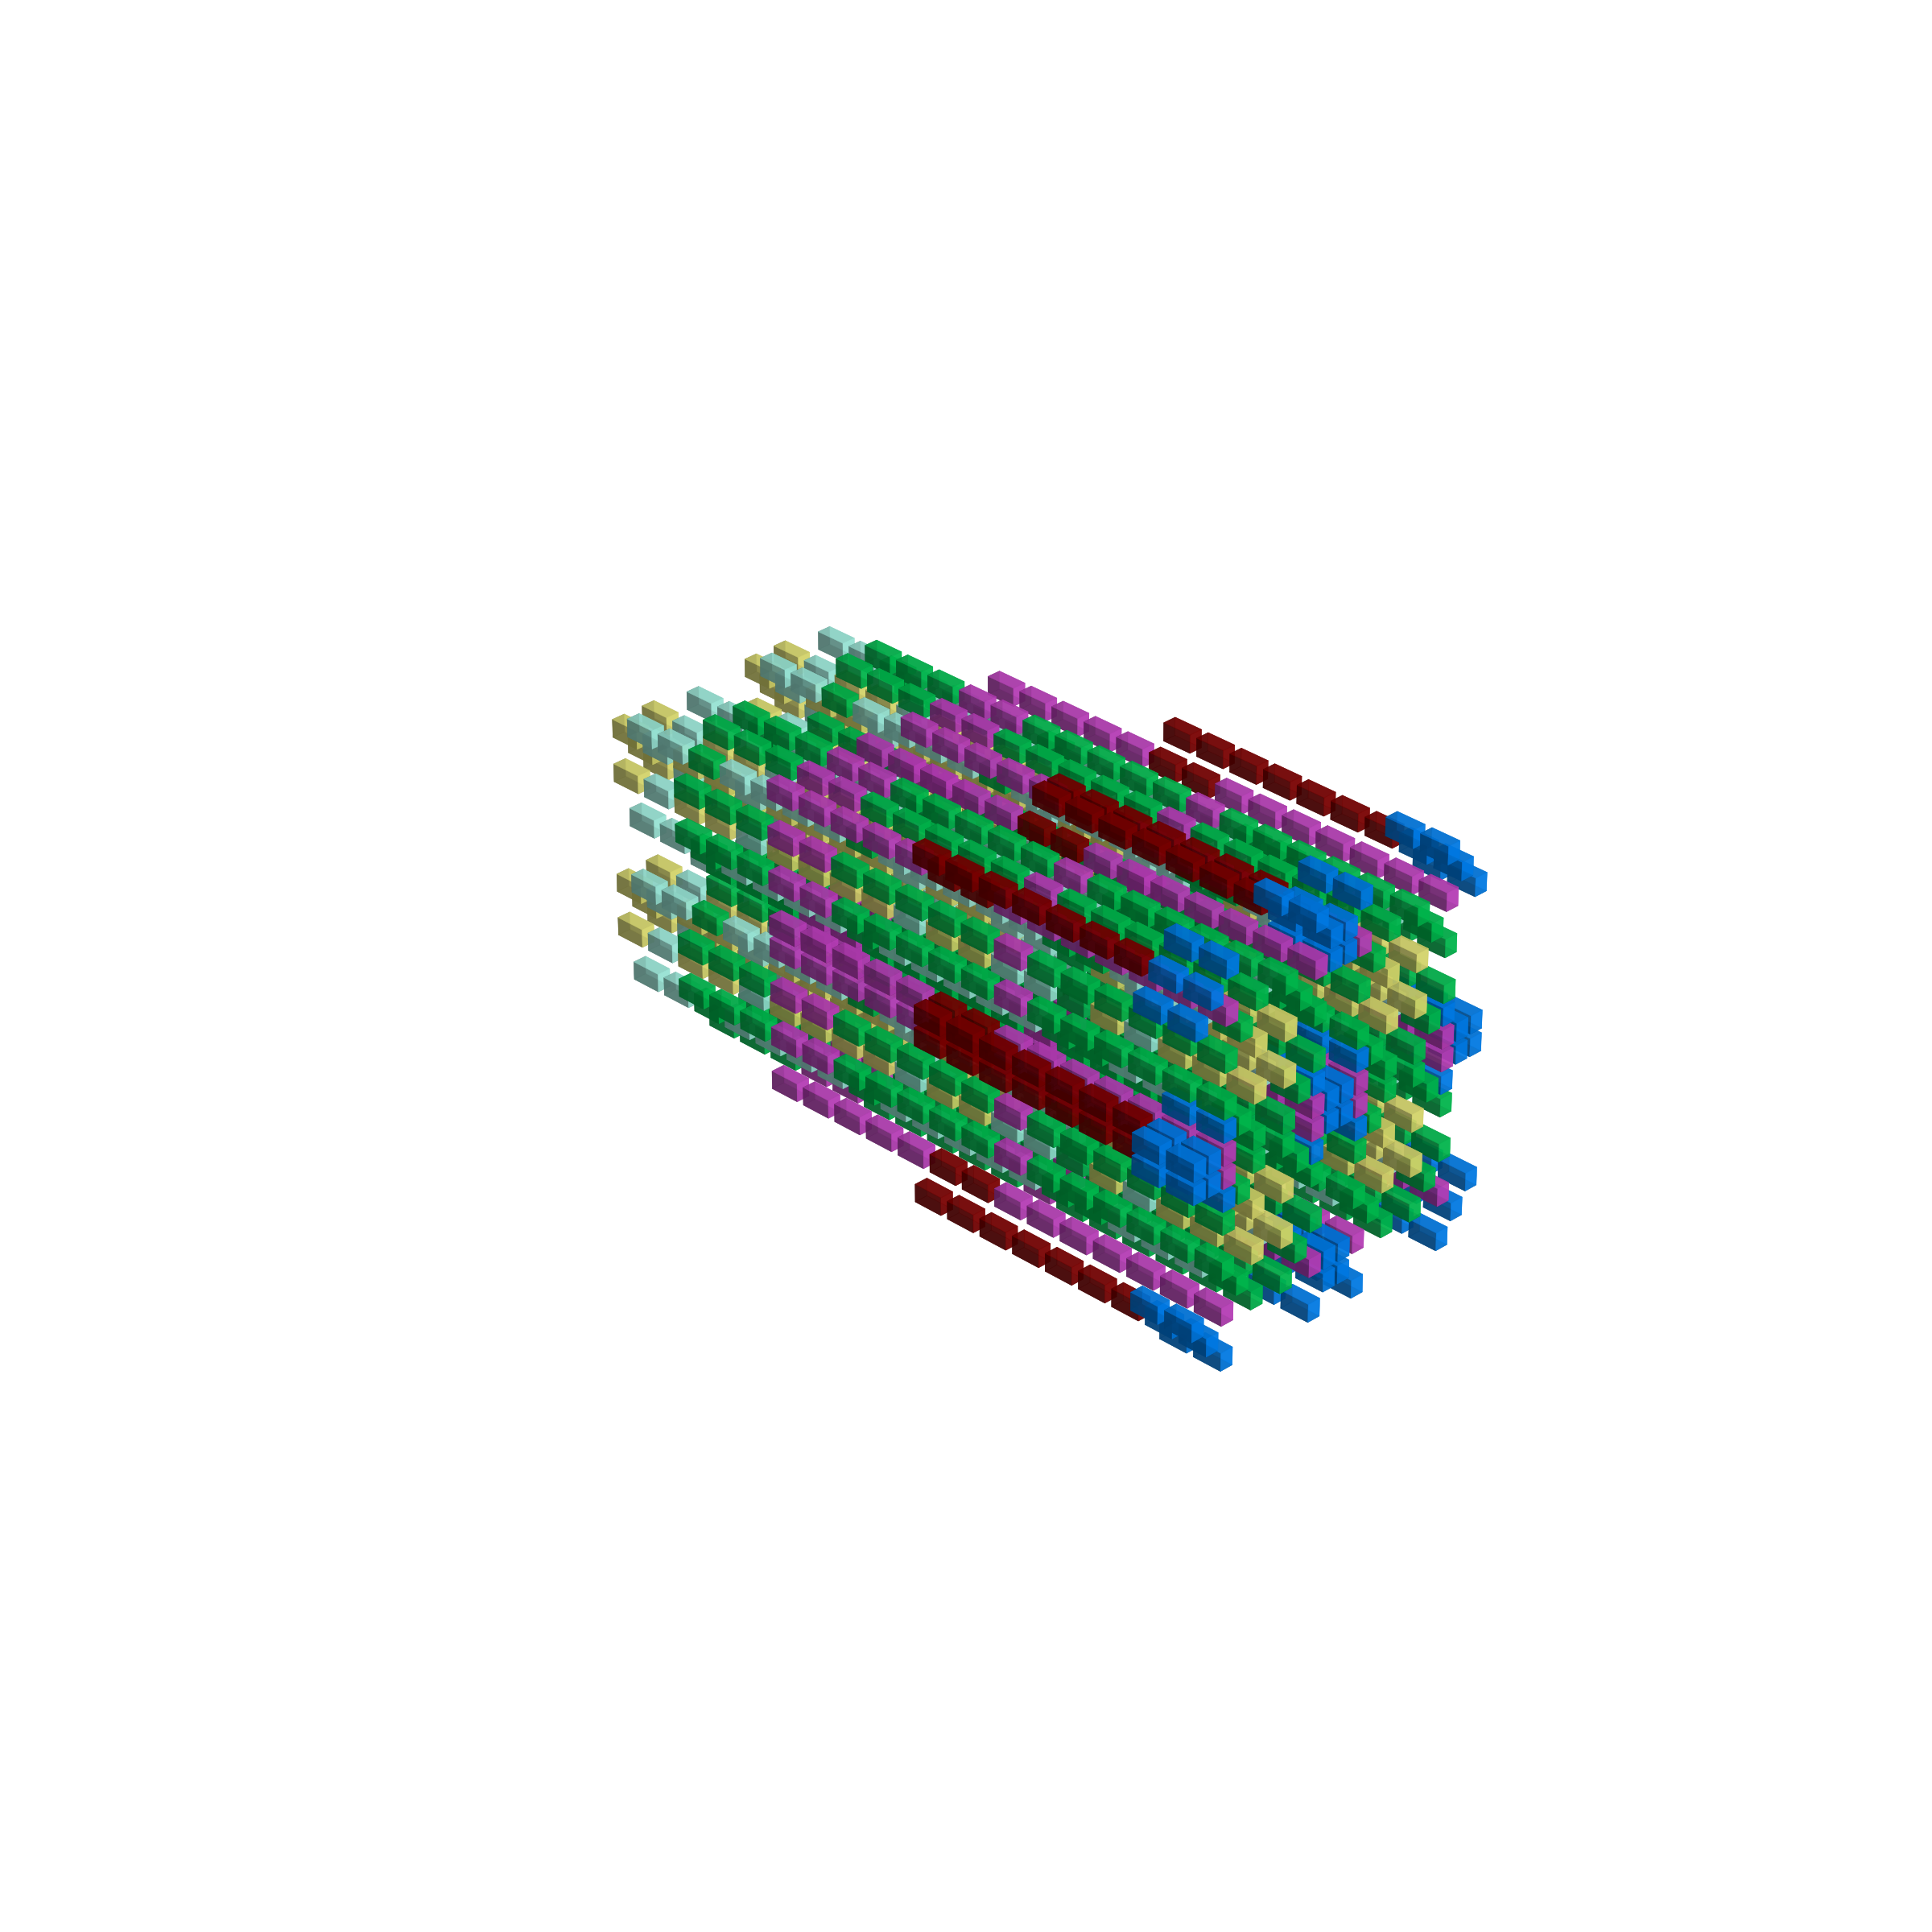
\includegraphics[width=8cm]{src/symmetries/pattern6_4-45.png}
        \vspace*{-2.5cm}
  \caption*{\getItem{6}}
  \end{figure}
\end{minipage}
\hspace{1cm}
\begin{minipage}[b]{0.50\linewidth}                                       
  \begin{figure}[H]
      \centering
        \vspace*{-1cm}
        \hspace*{-2cm}
        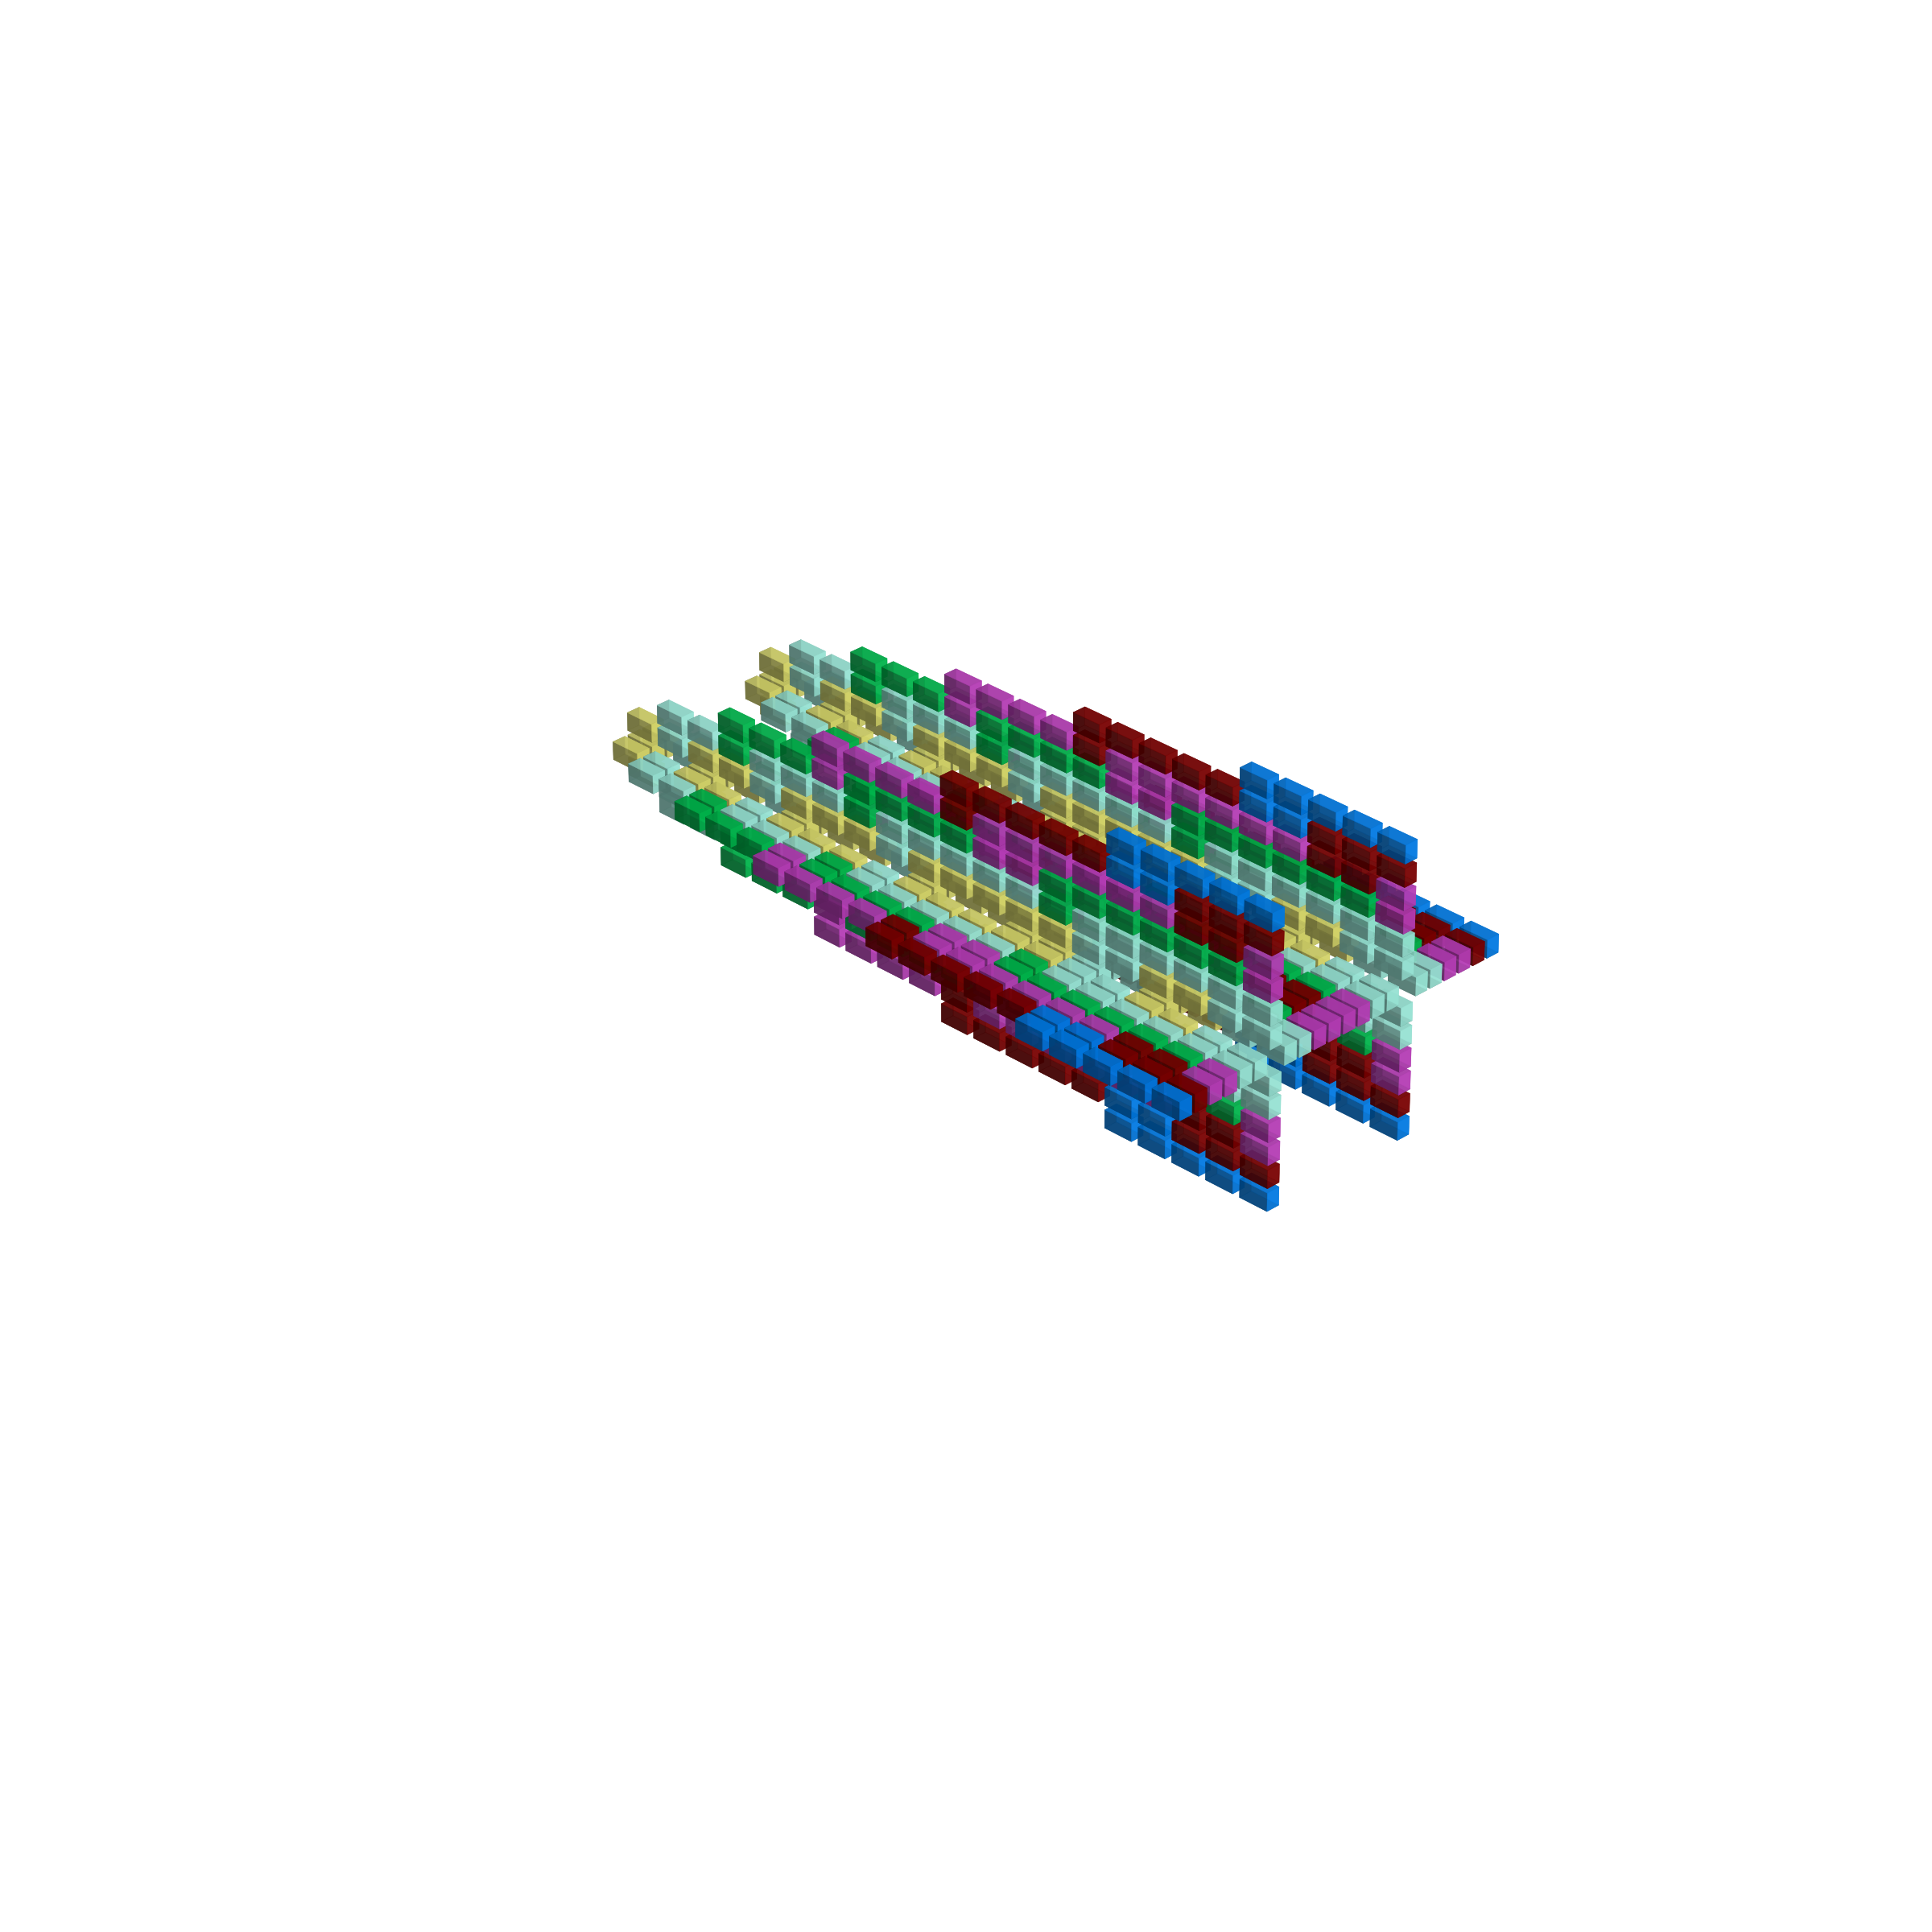
\includegraphics[width=8cm]{src/symmetries/pattern7_1-45.png}%
        \hspace*{-4cm}
        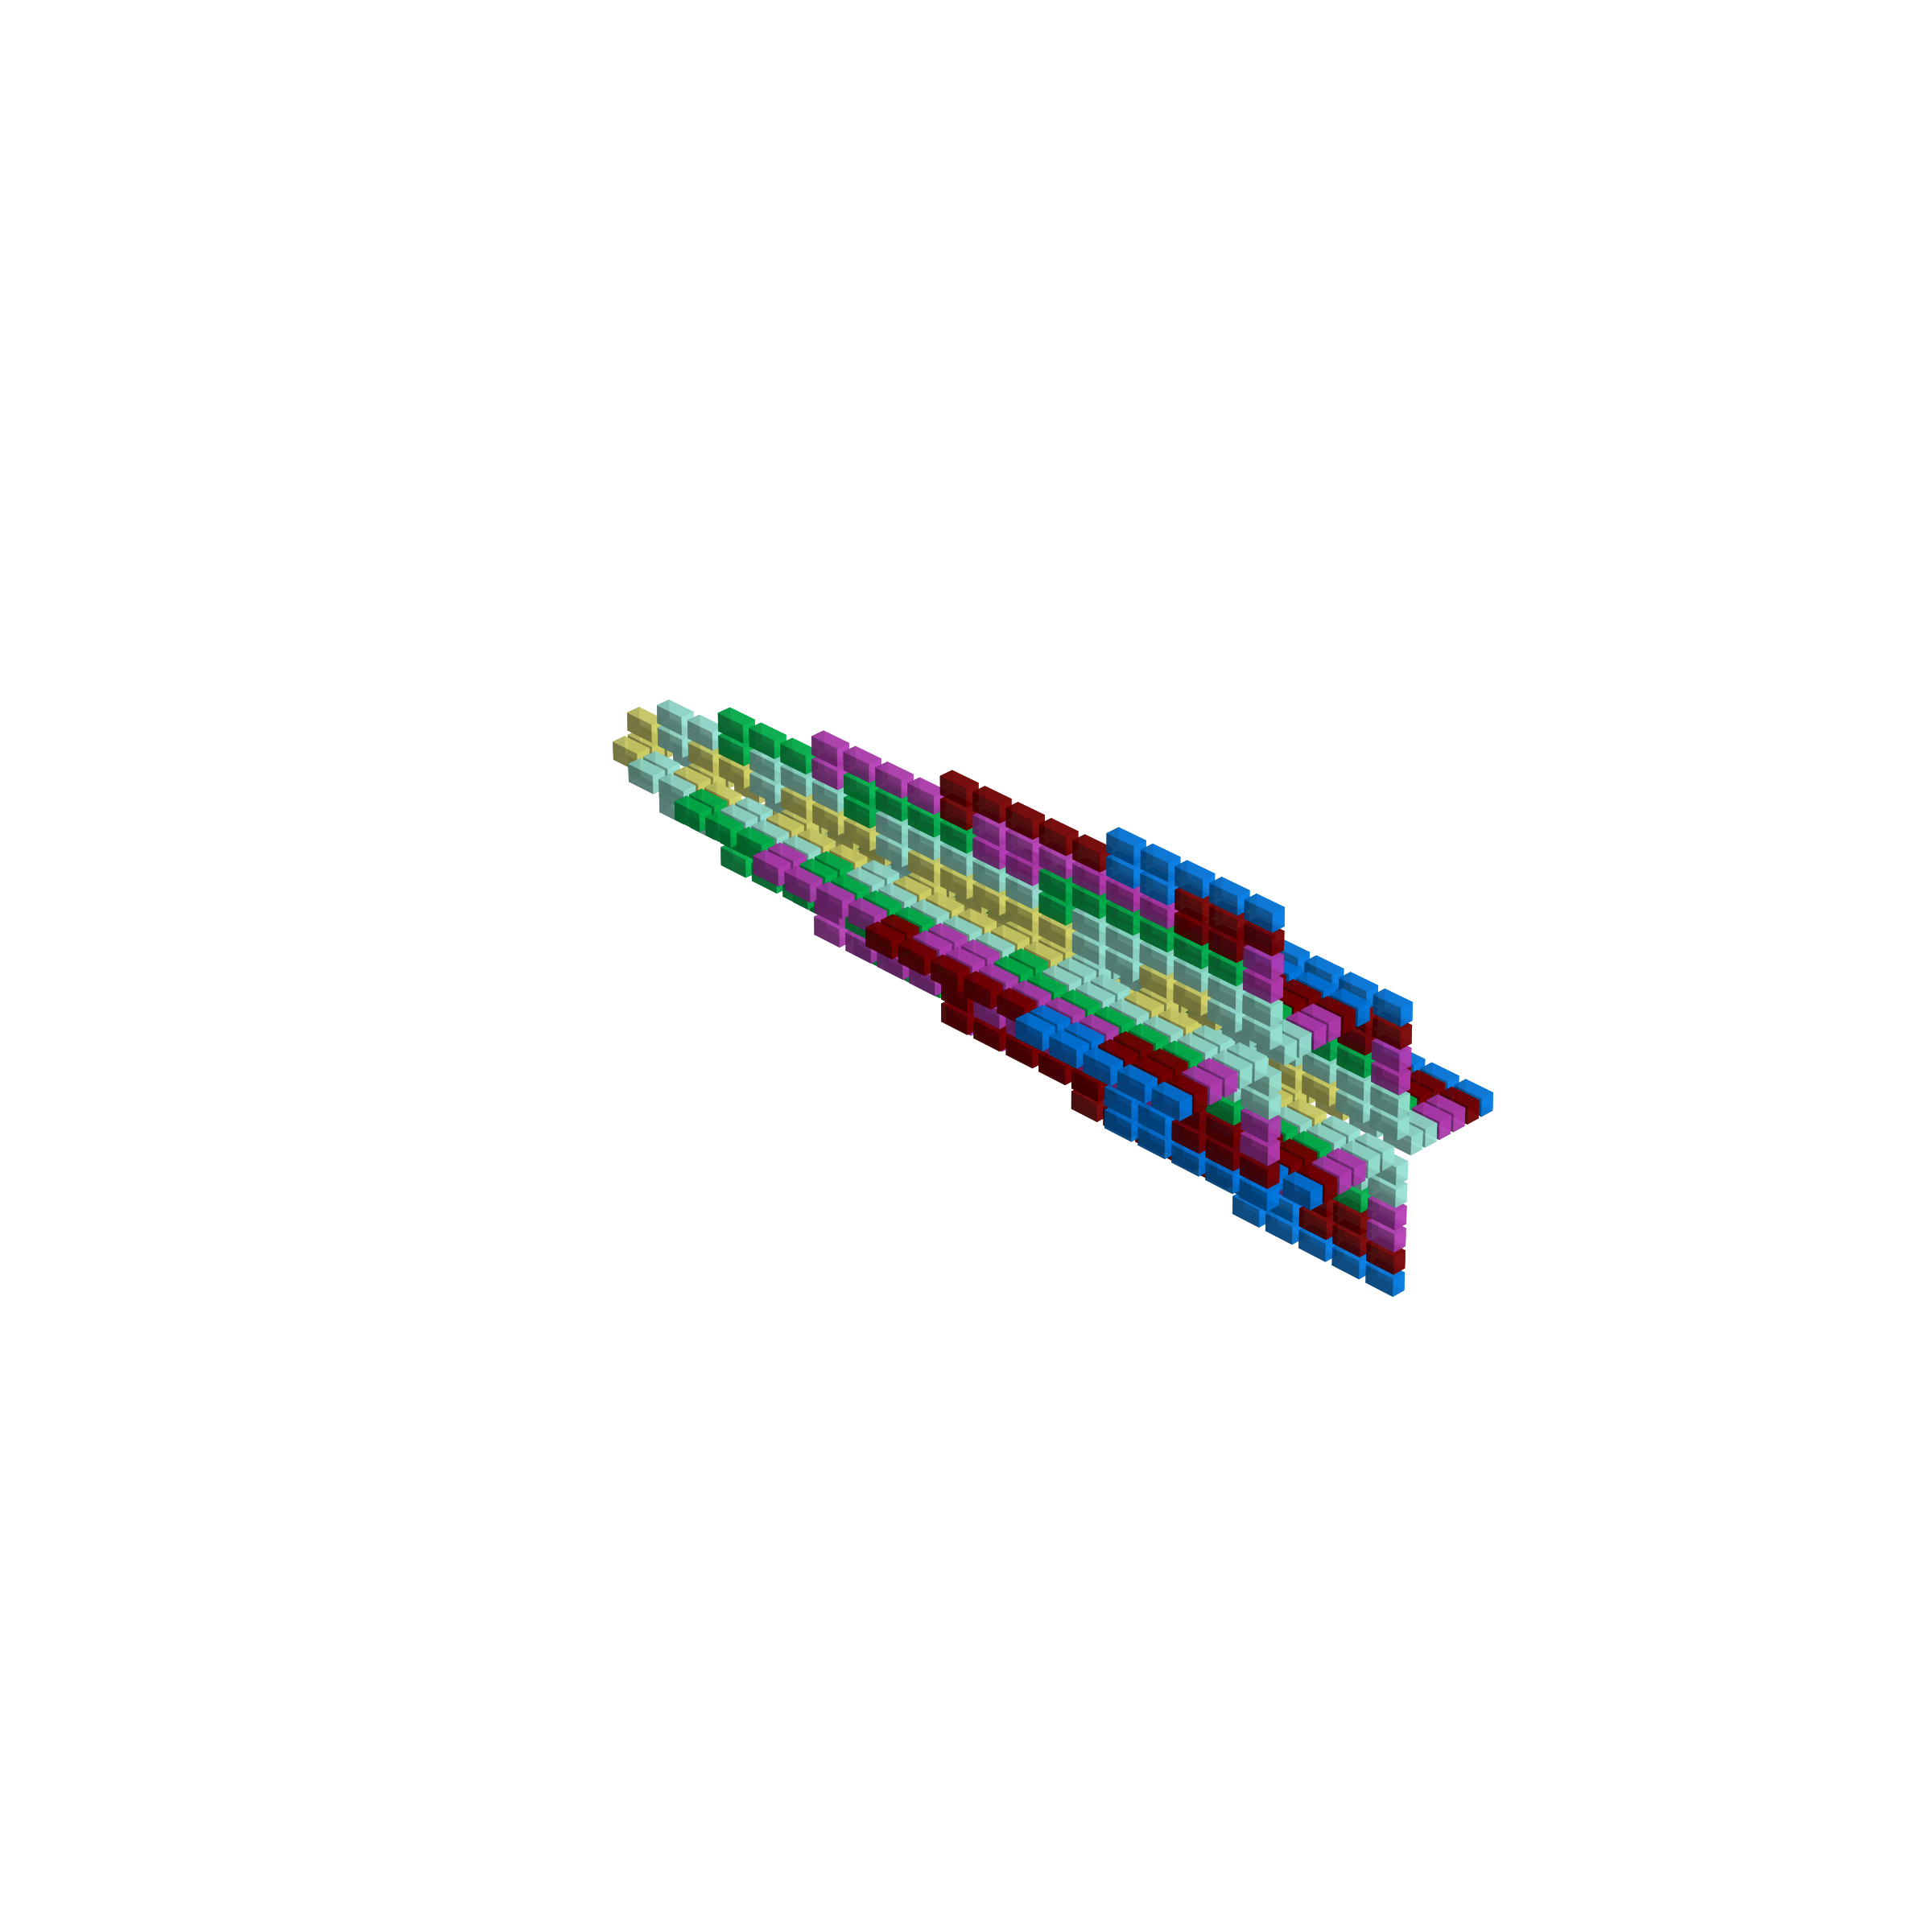
\includegraphics[width=8cm]{src/symmetries/pattern7_2-45.png}\\
        \vspace*{-5cm}
        \hspace*{-1cm}
        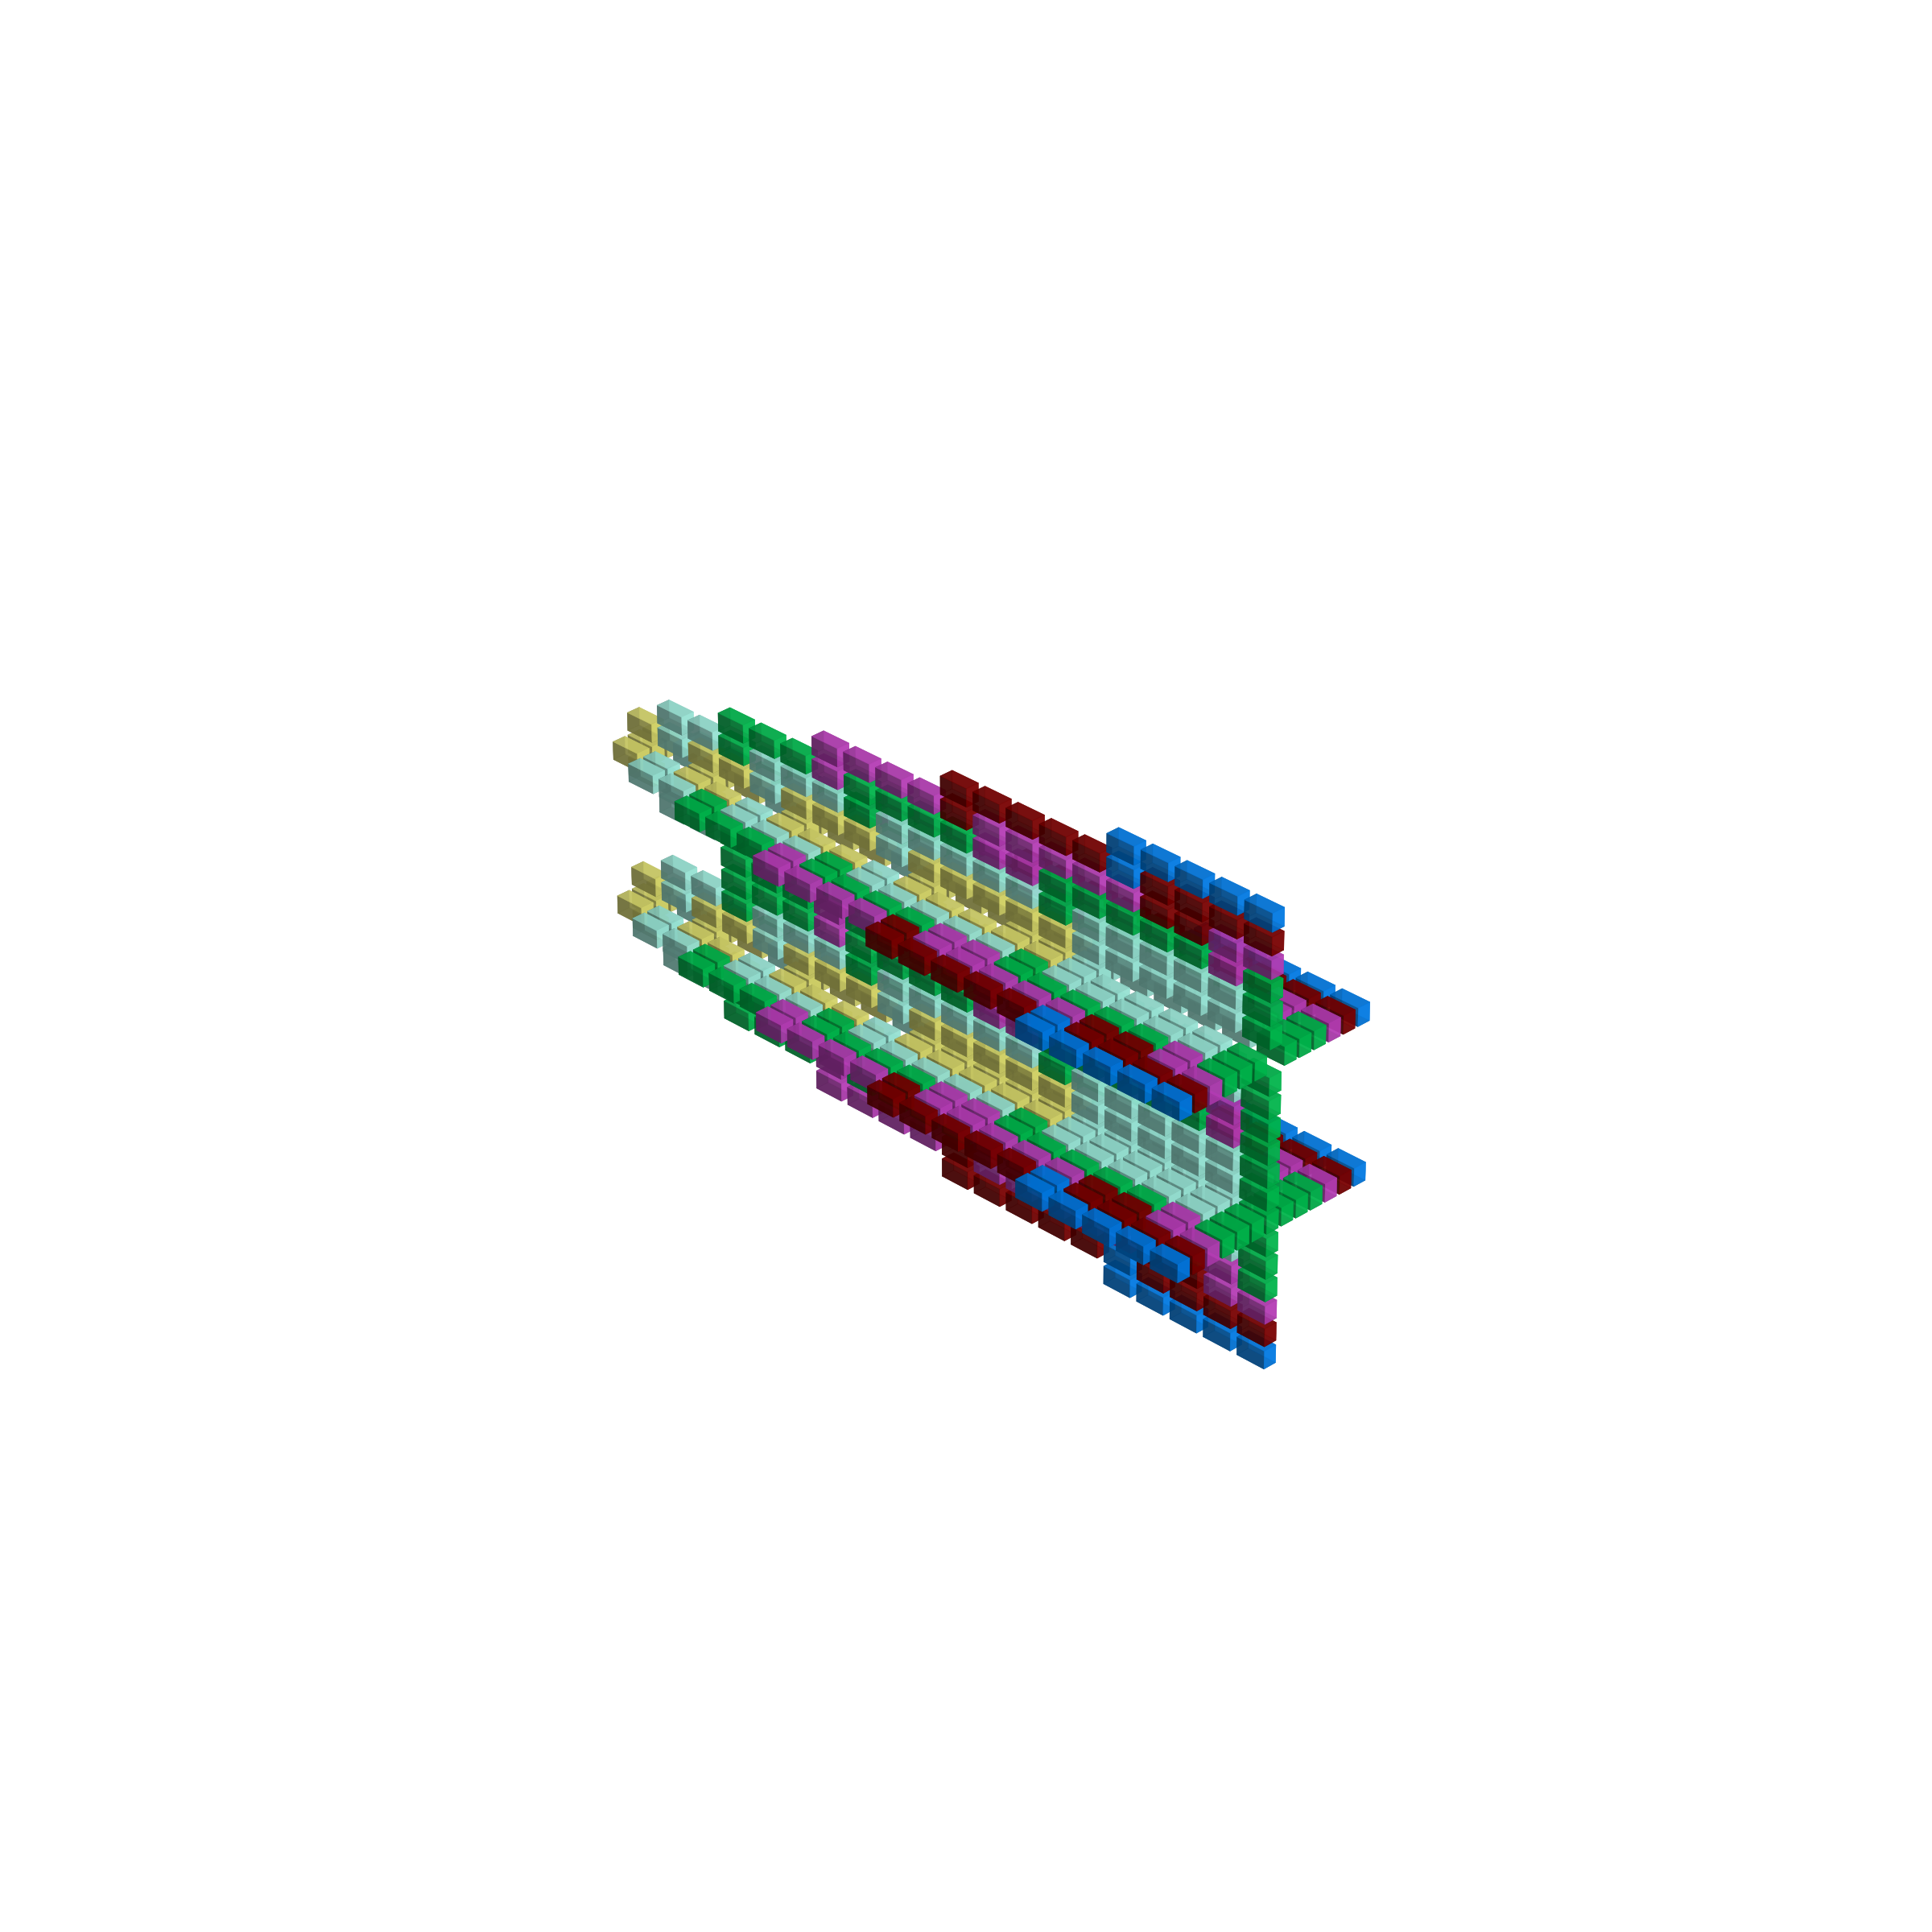
\includegraphics[width=8cm]{src/symmetries/pattern7_3-45.png}\\
        \vspace*{-8cm}
        \hspace*{2cm}
        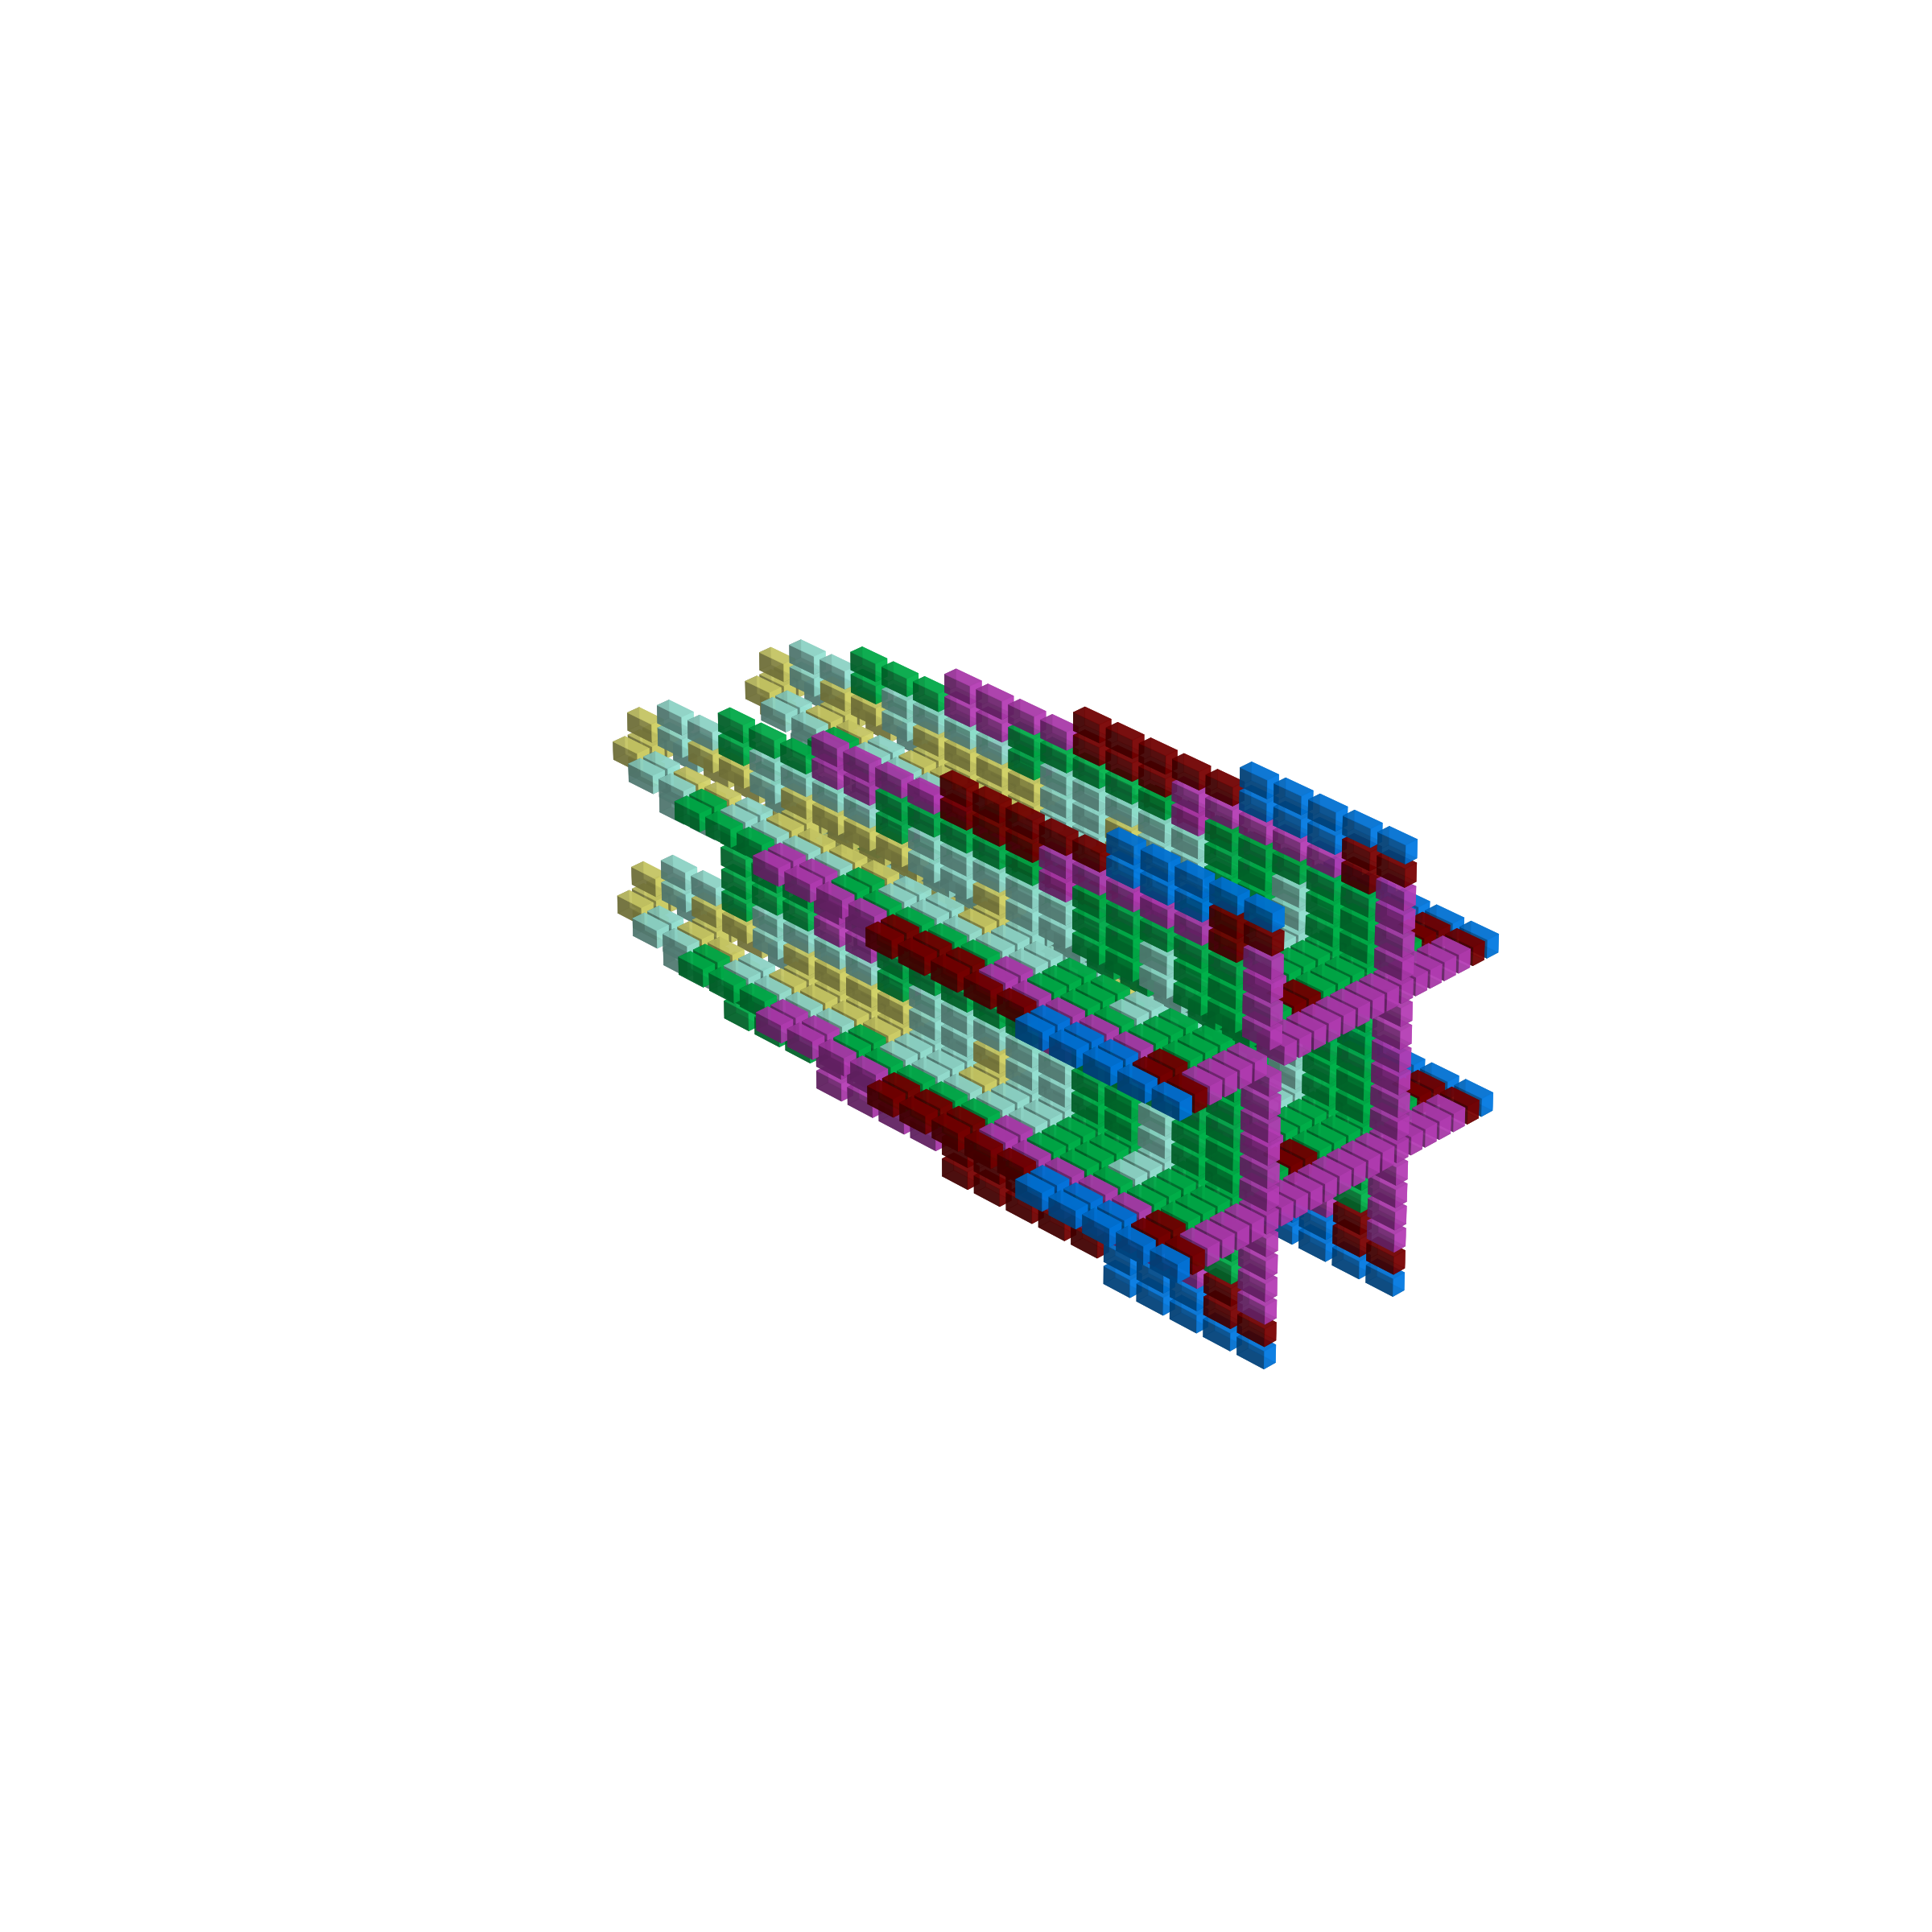
\includegraphics[width=8cm]{src/symmetries/pattern7_4-45.png}
        \vspace*{-2.5cm}
  \caption*{\getItem{7}}
  \end{figure}
\end{minipage}
\begin{minipage}[b]{0.50\linewidth}                                       
  \begin{figure}[H]
      \centering
        \vspace*{-1cm}
        \hspace*{-2cm}
        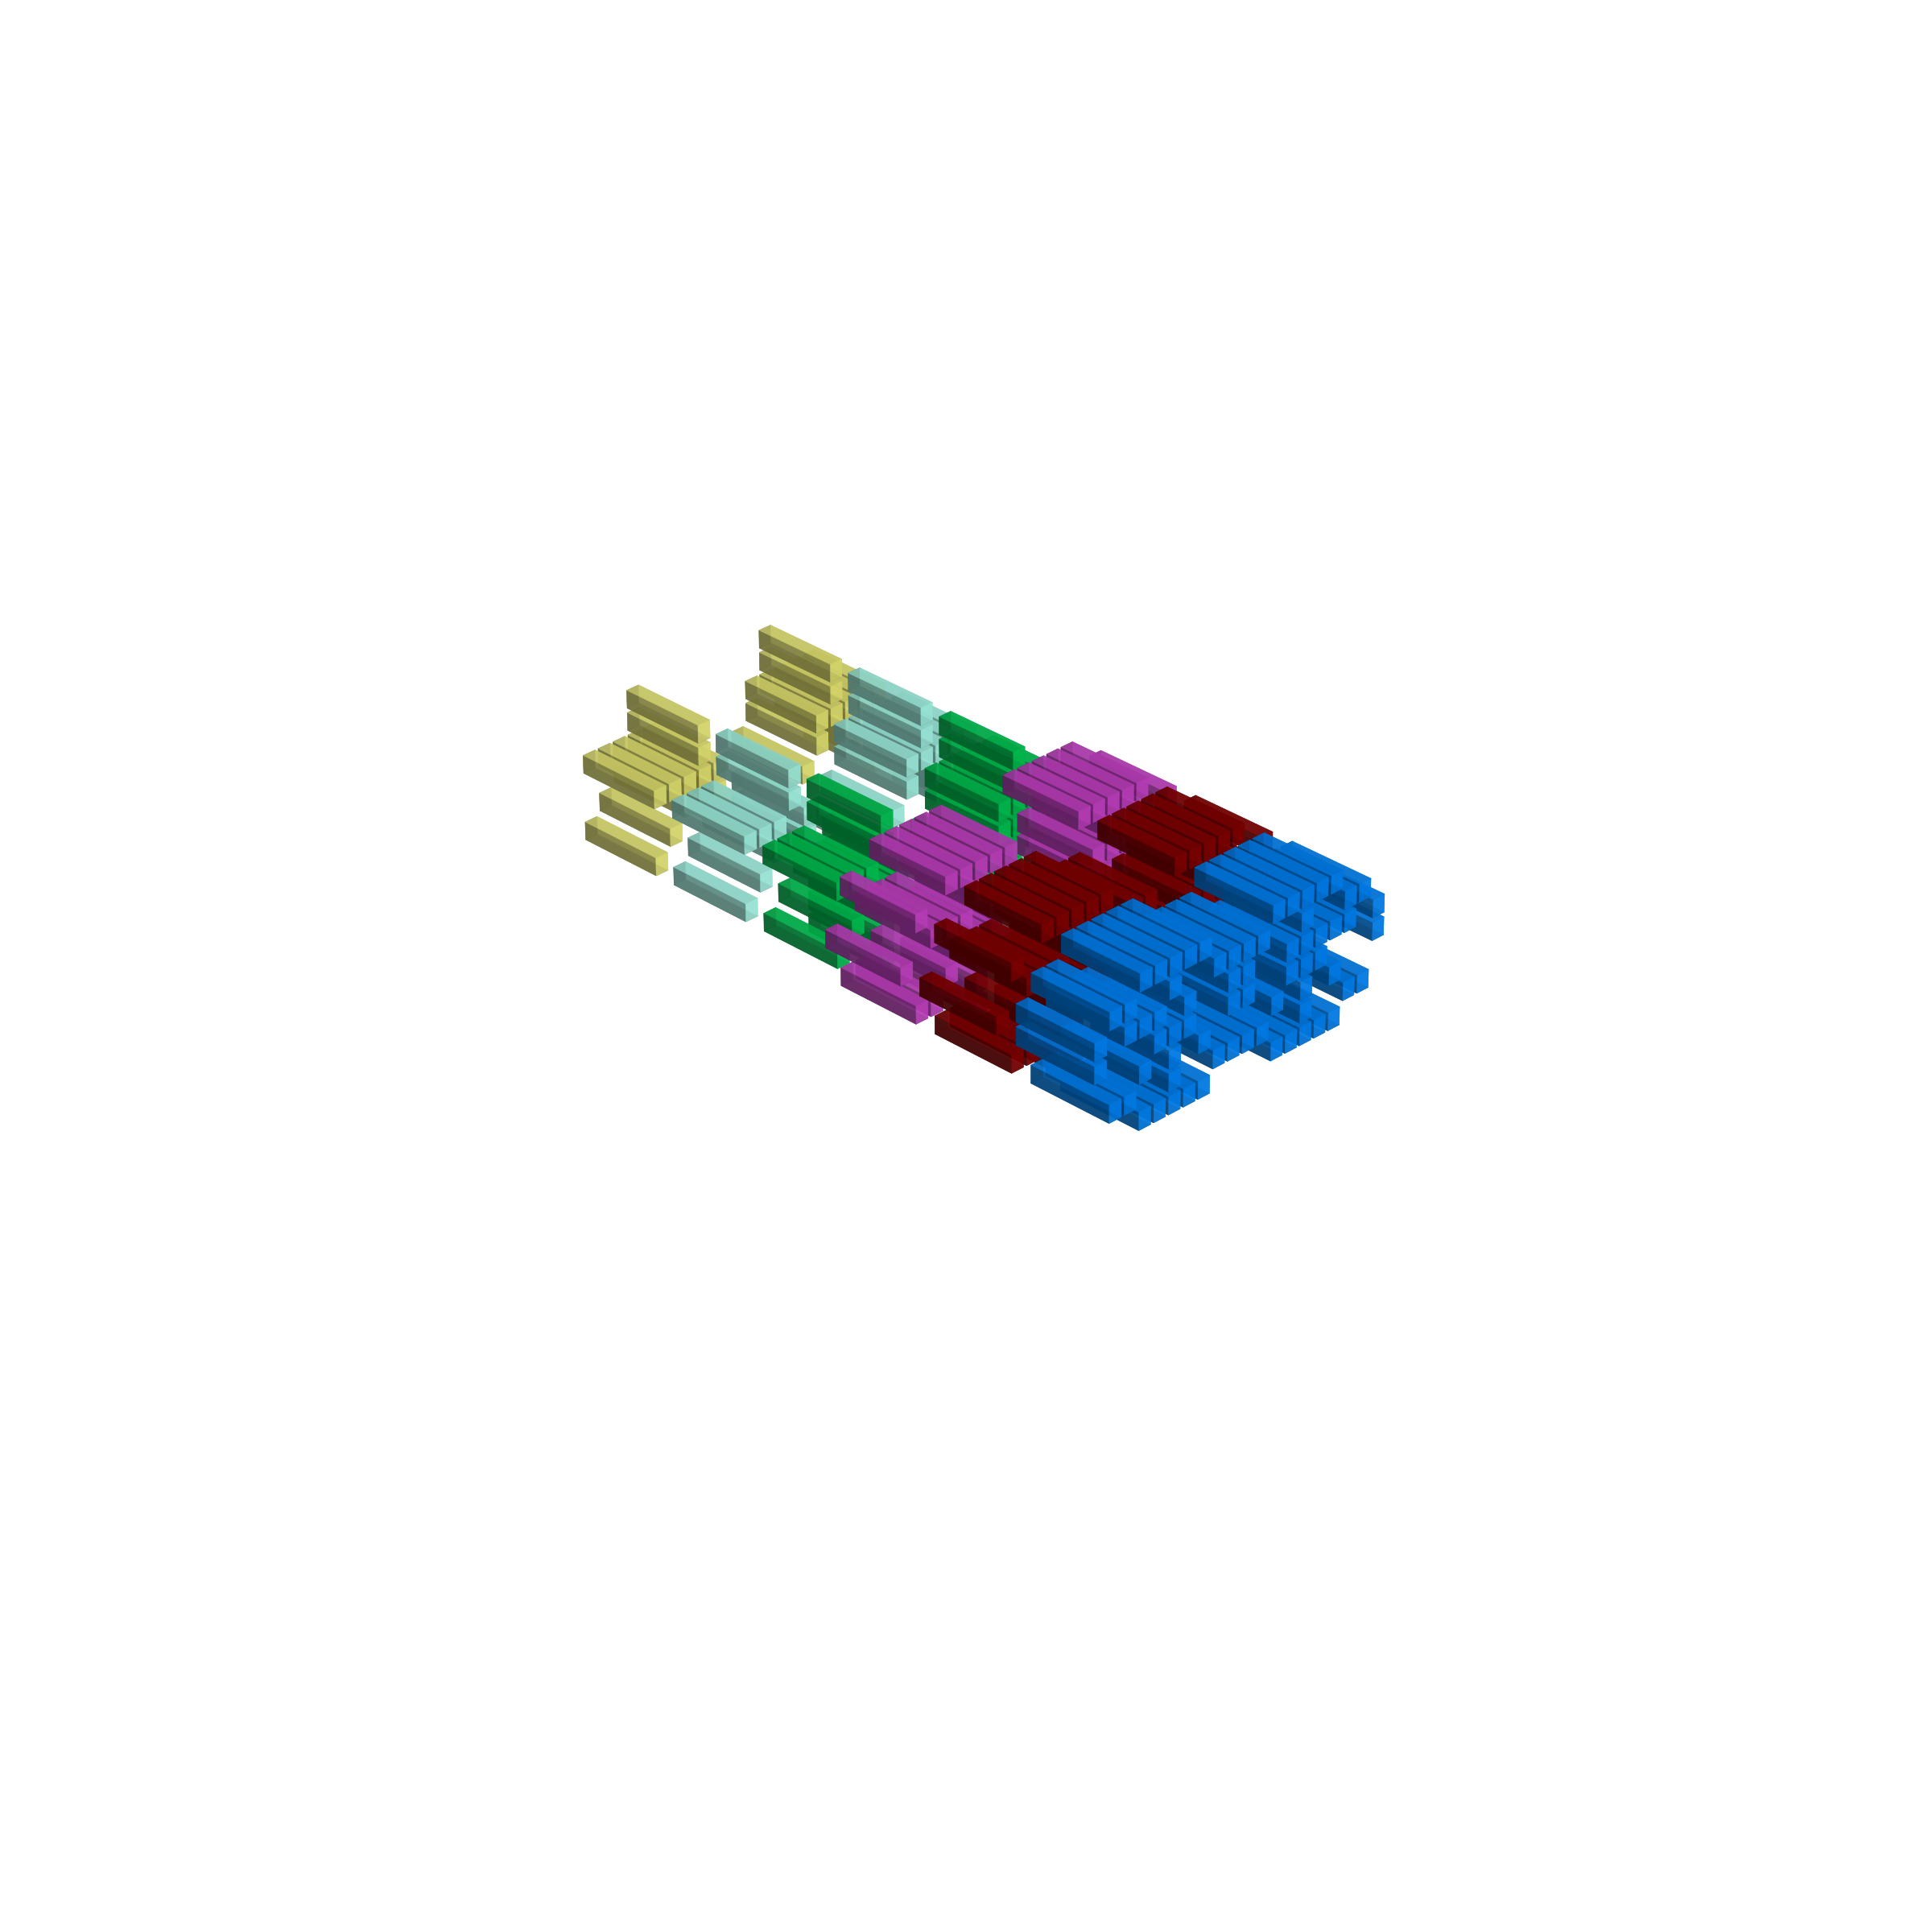
\includegraphics[width=8cm]{src/symmetries/pattern8_1-45.png}%
        \hspace*{-4cm}
        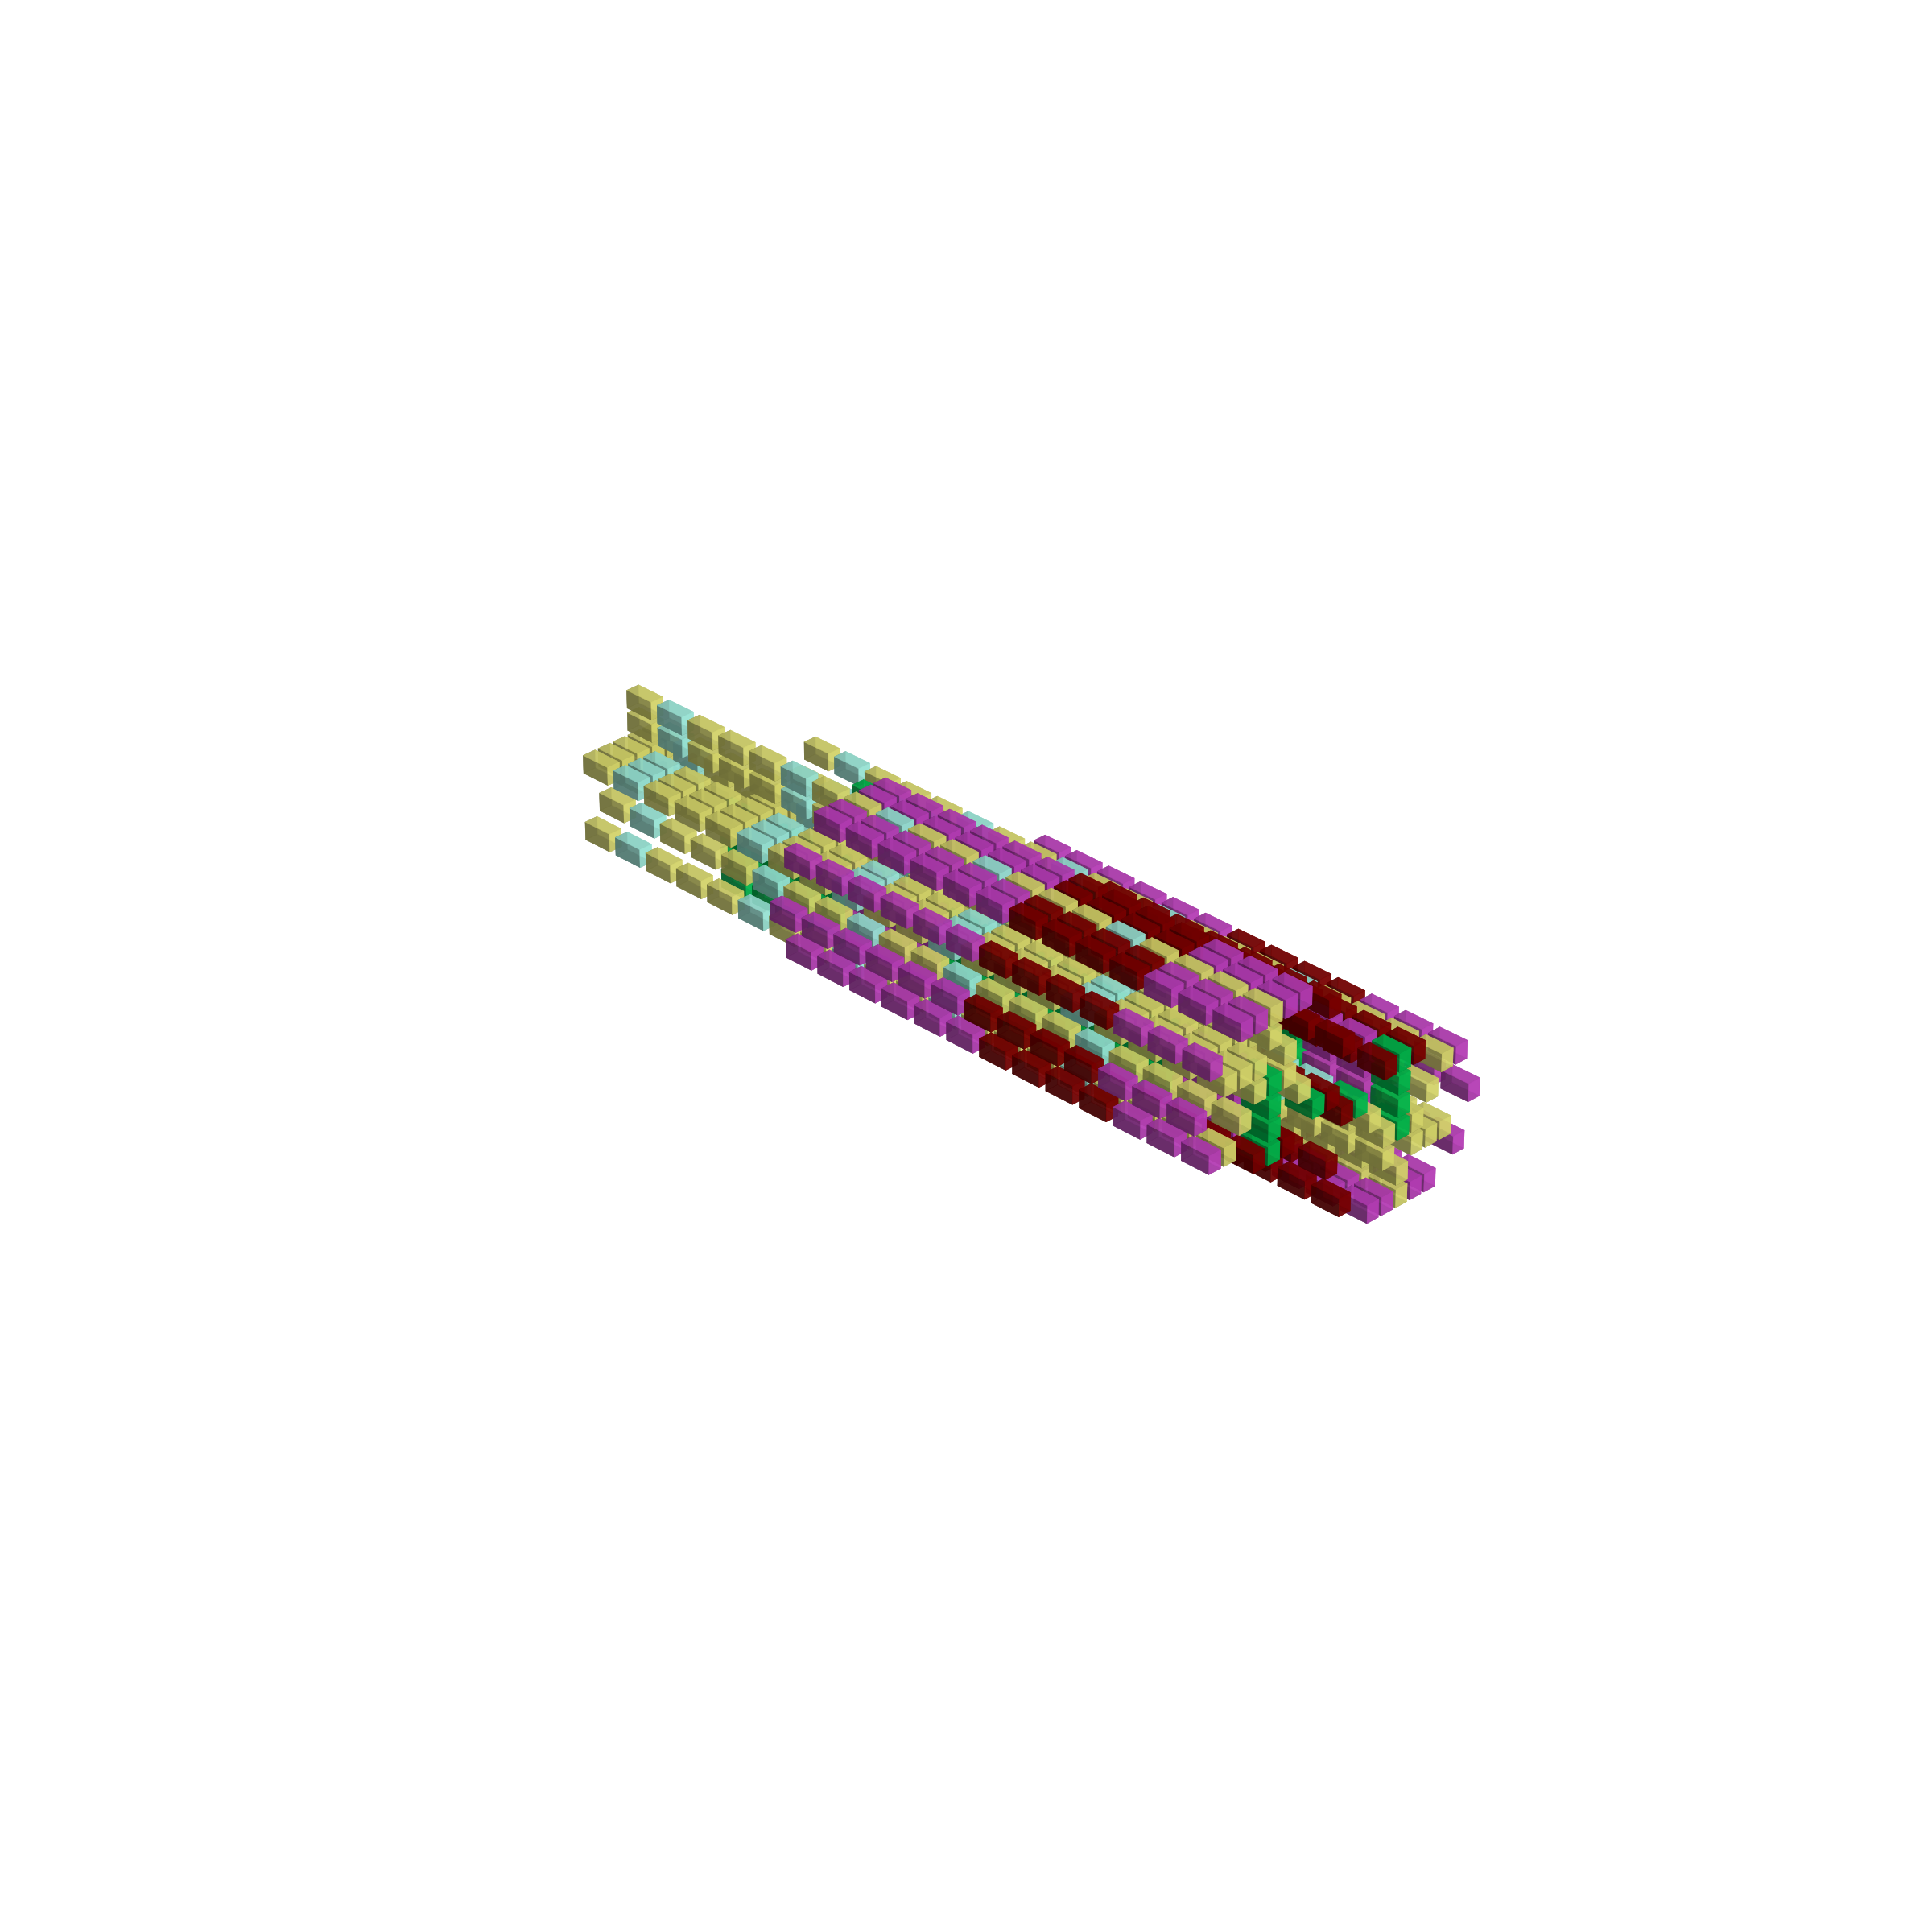
\includegraphics[width=8cm]{src/symmetries/pattern8_2-45.png}\\
        \vspace*{-5cm}
        \hspace*{-3cm}
        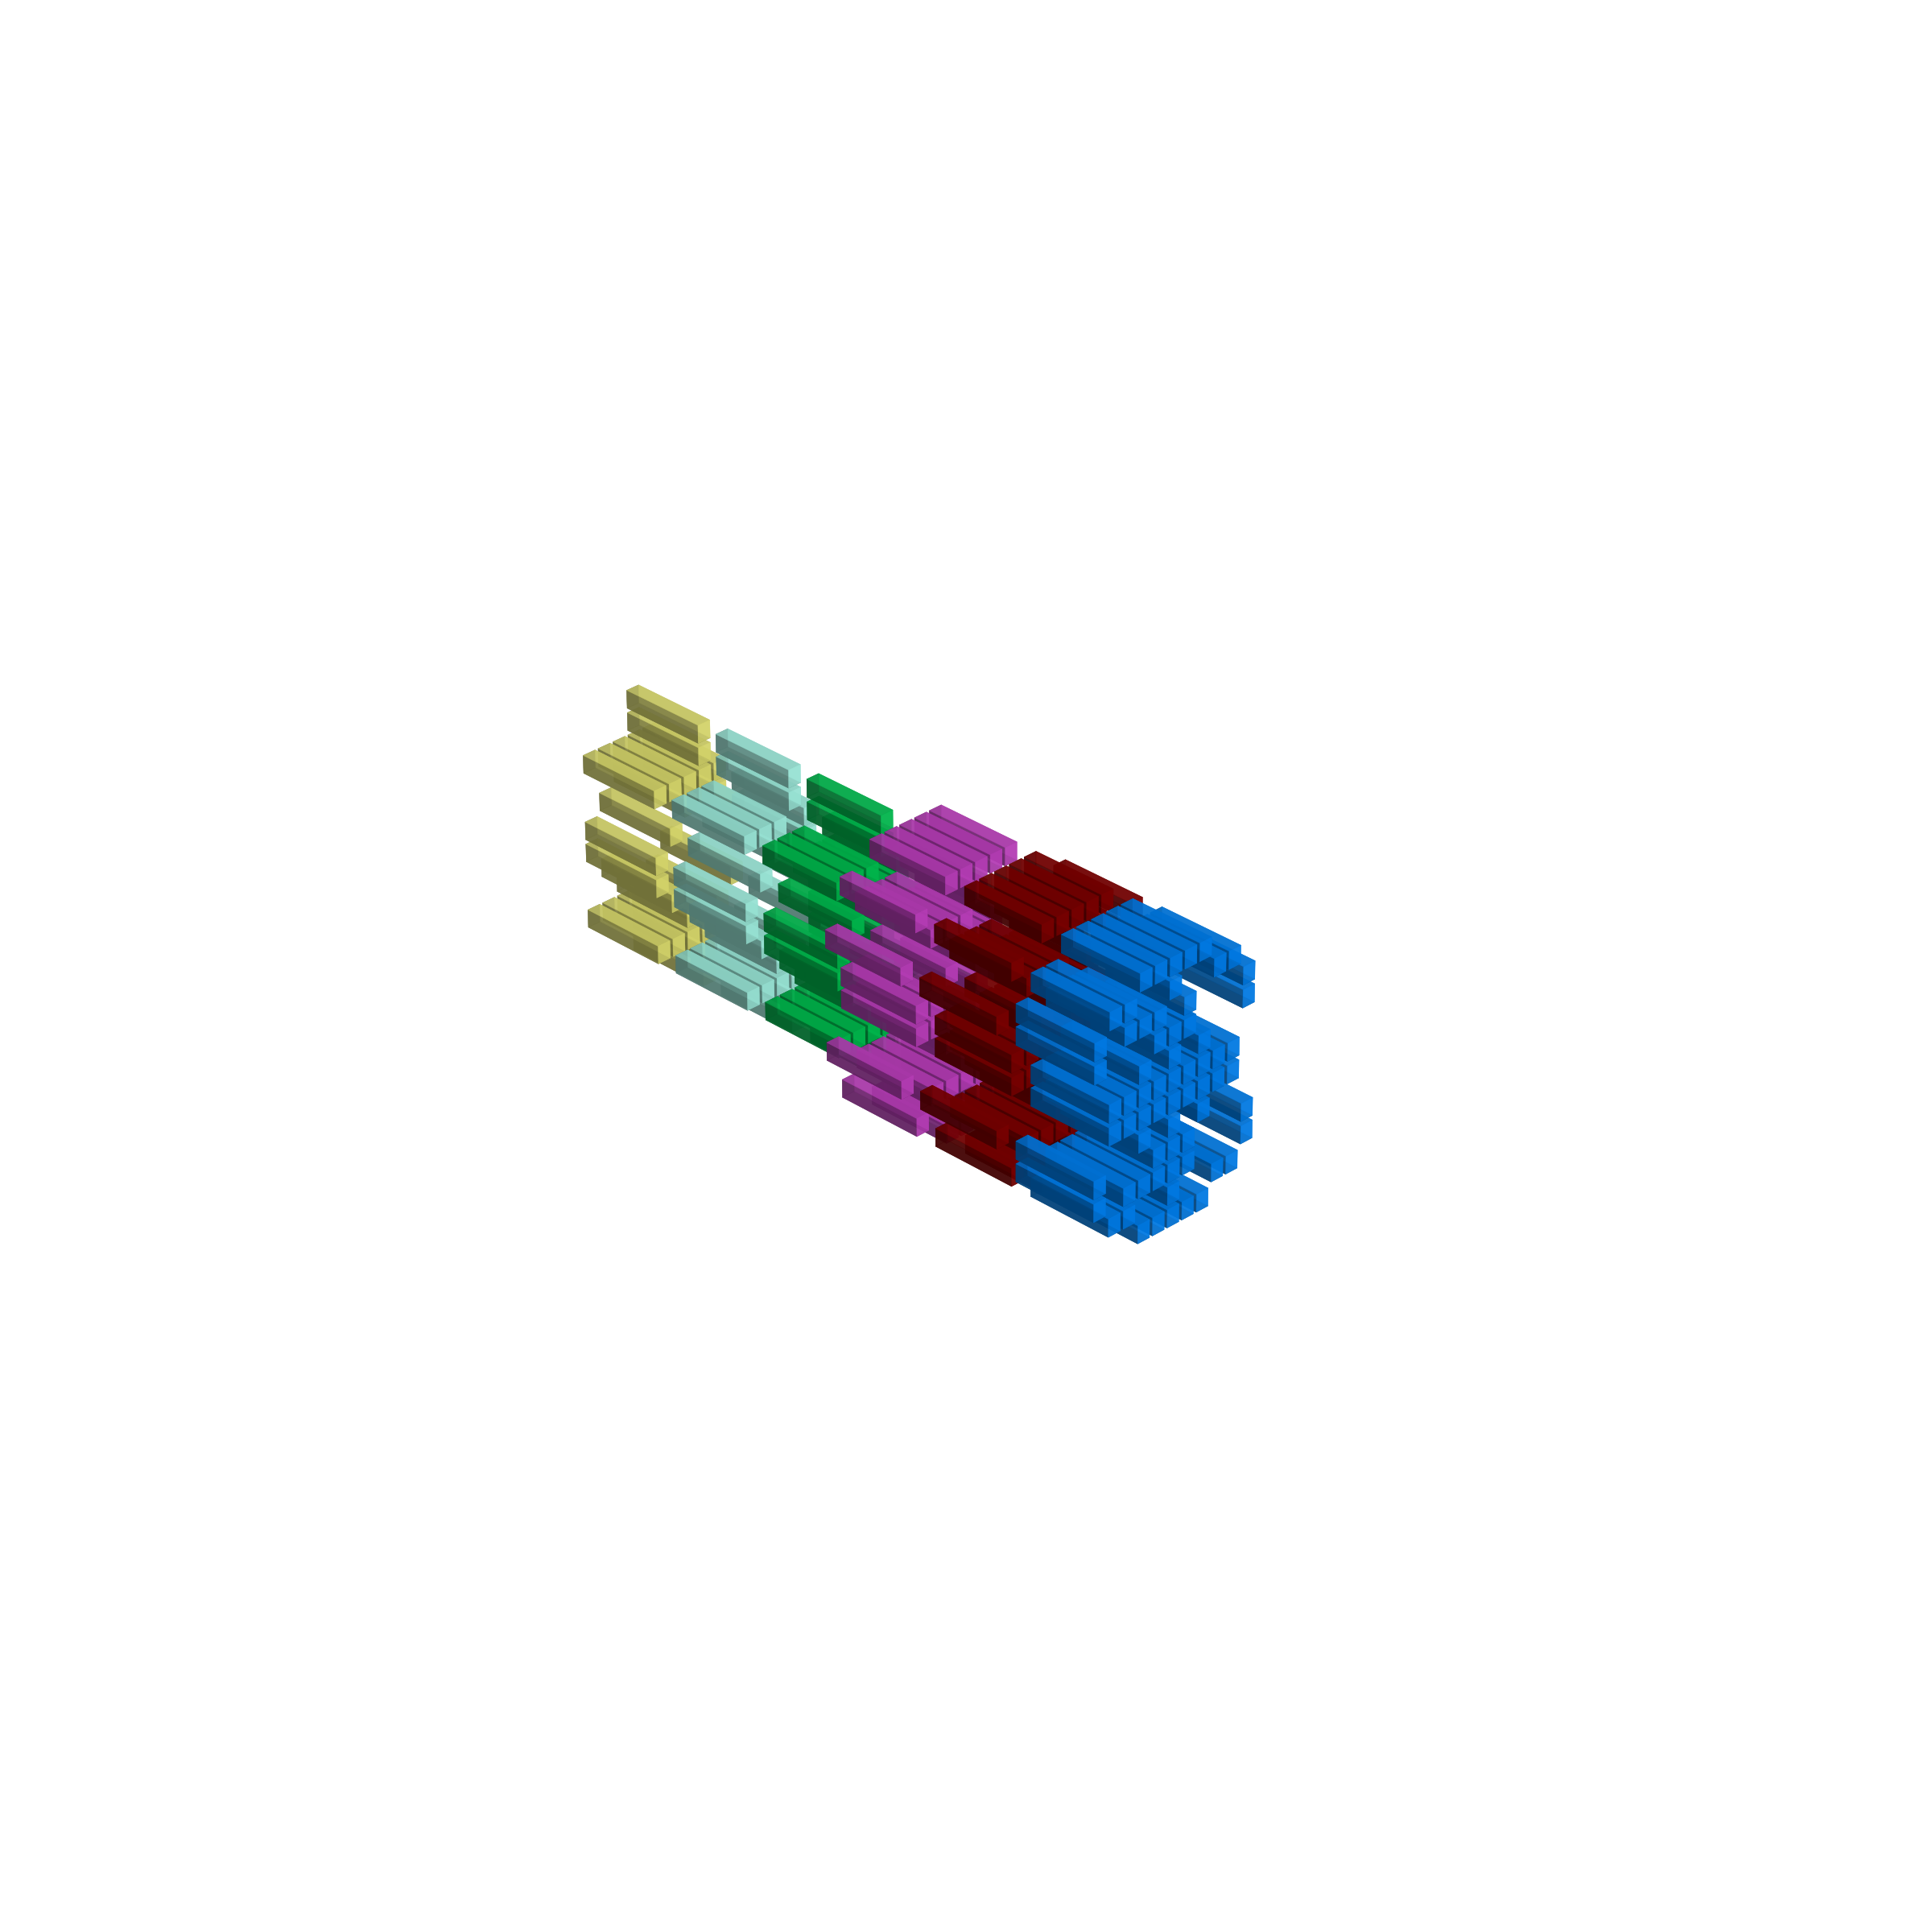
\includegraphics[width=8cm]{src/symmetries/pattern8_3-45.png}\\
        \vspace*{-8cm}
        \hspace*{2cm}
        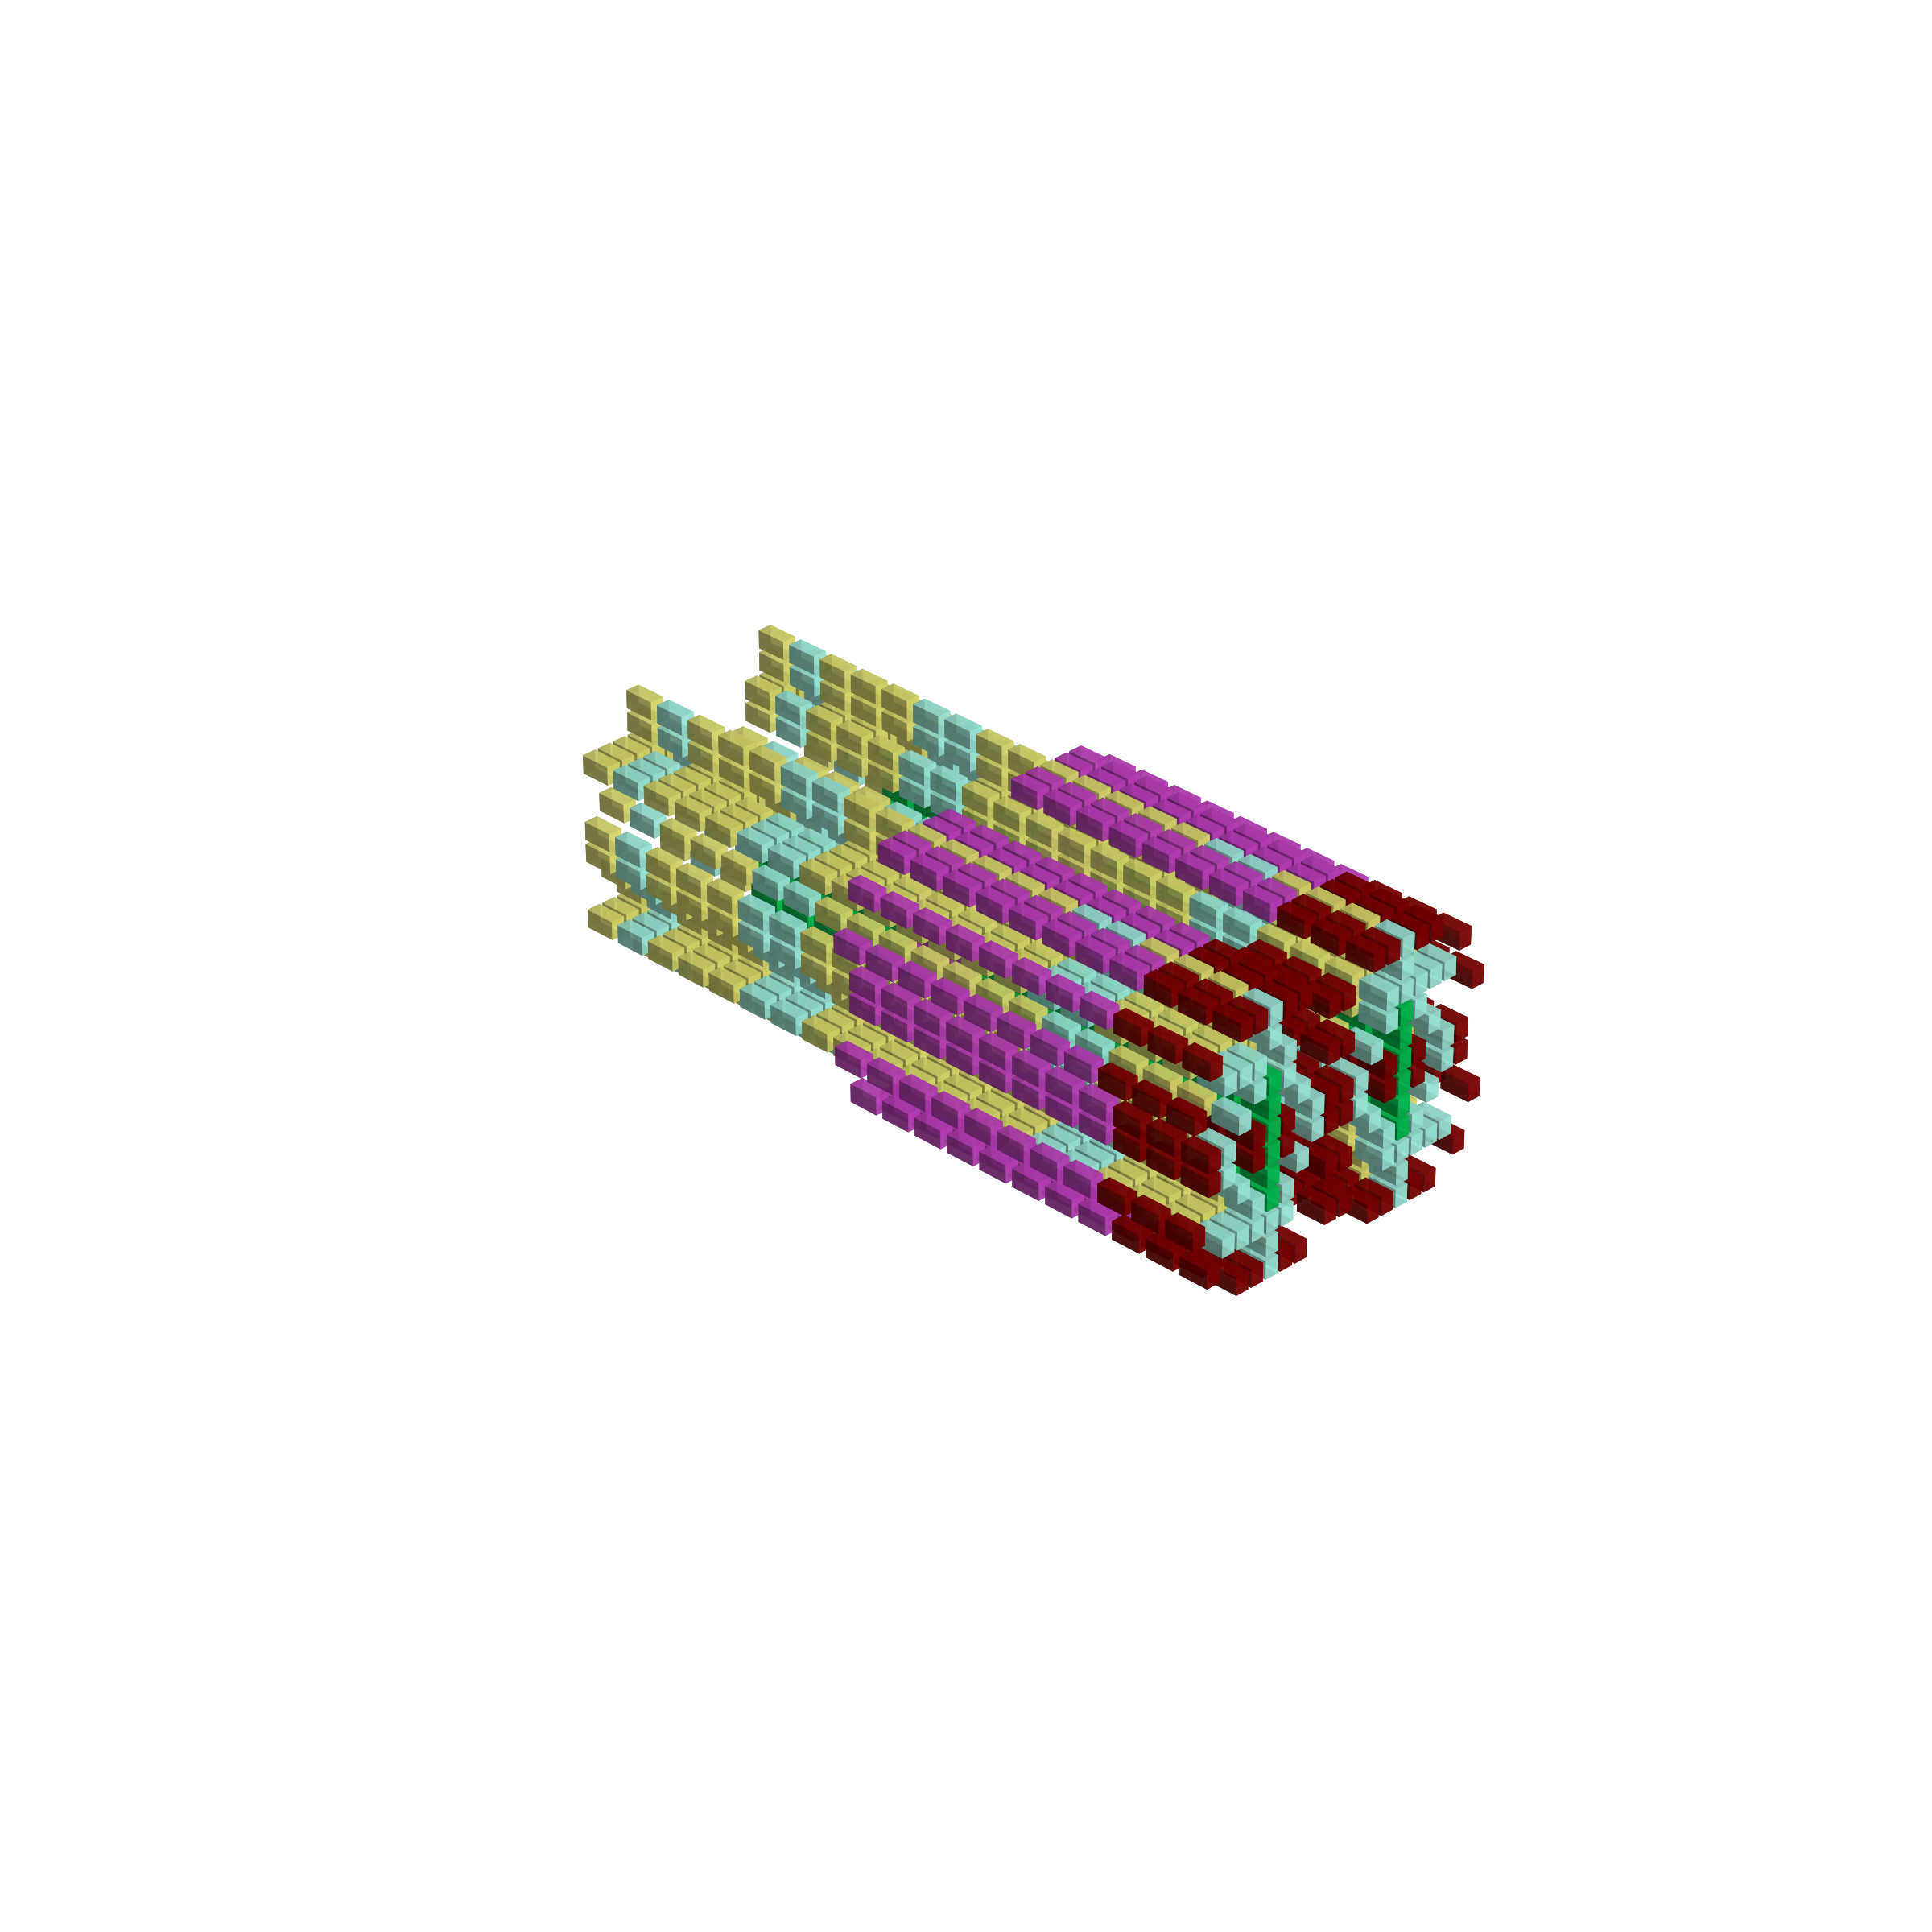
\includegraphics[width=8cm]{src/symmetries/pattern8_4-45.png}
        \vspace*{-2.5cm}
  \caption*{\getItem{8}}
  \end{figure}
\end{minipage}
\hspace{1cm}
\begin{minipage}[b]{0.50\linewidth}                                       
  \begin{figure}[H]
      \centering
        \vspace*{-1cm}
        \hspace*{-2cm}
        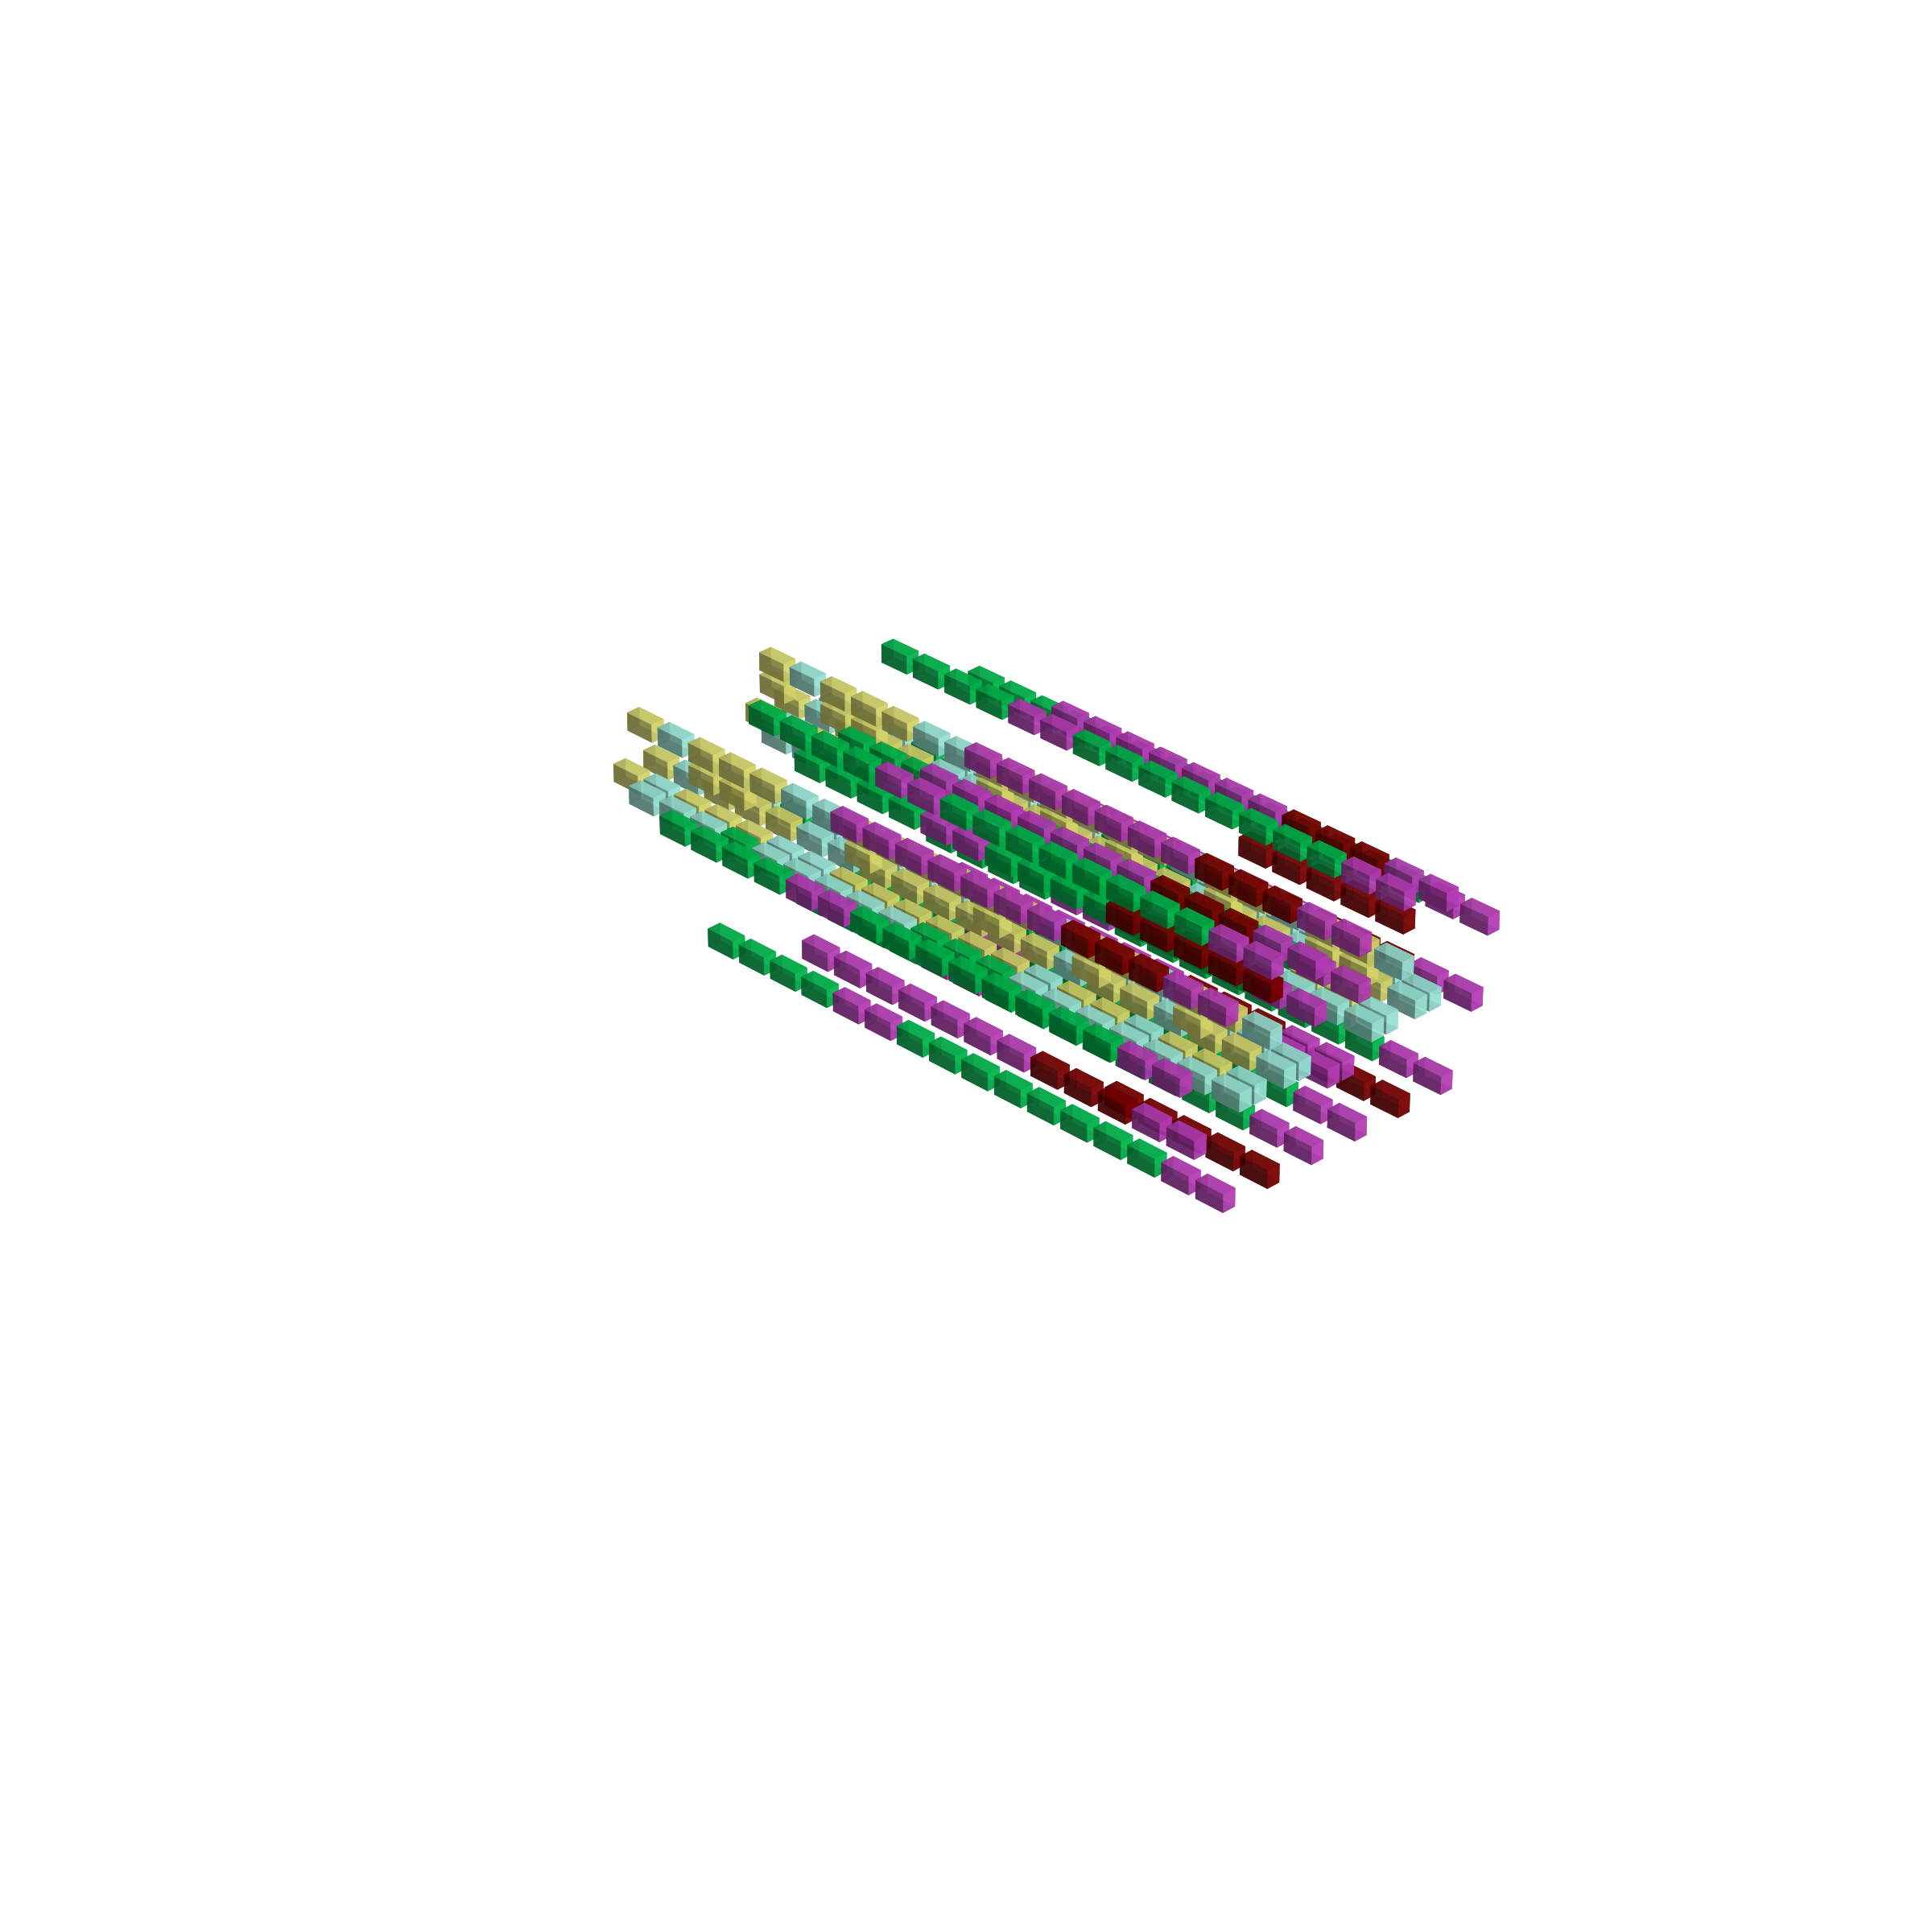
\includegraphics[width=8cm]{src/symmetries/pattern9_1-45.png}%
        \hspace*{-4cm}
        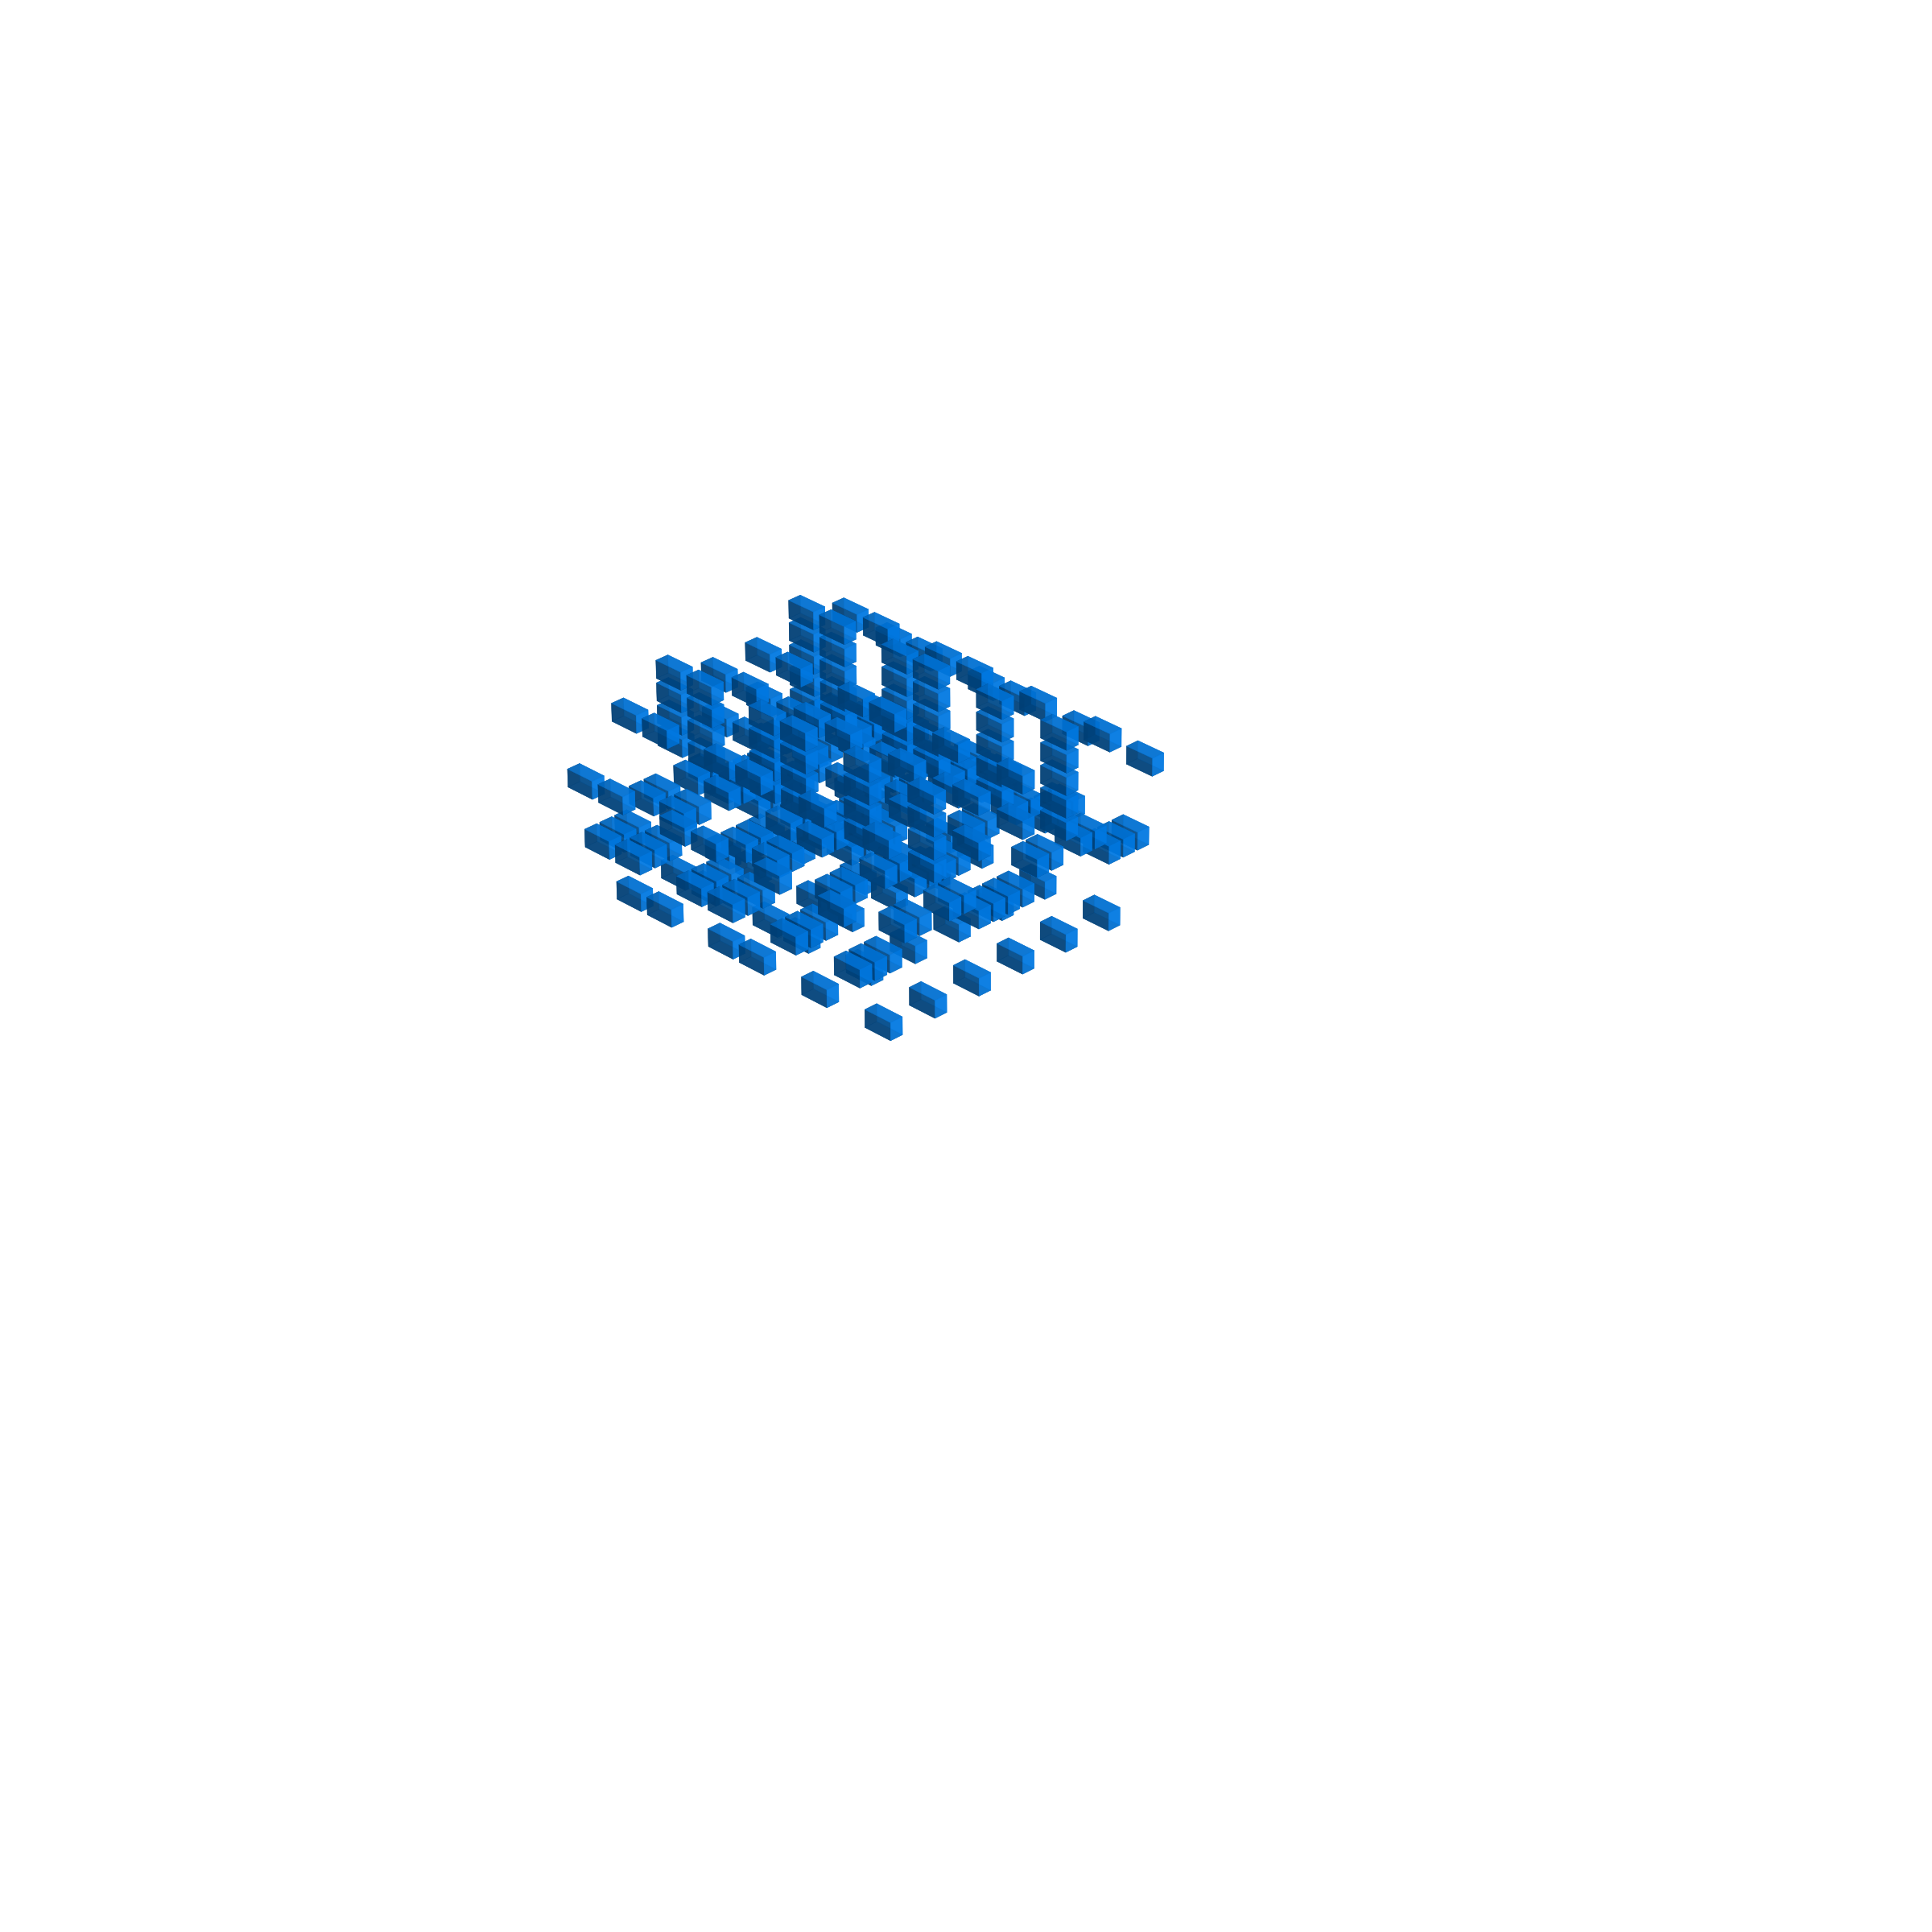
\includegraphics[width=8cm]{src/symmetries/pattern9_2-45.png}\\
        \vspace*{-5cm}
        \hspace*{-1.5cm}
        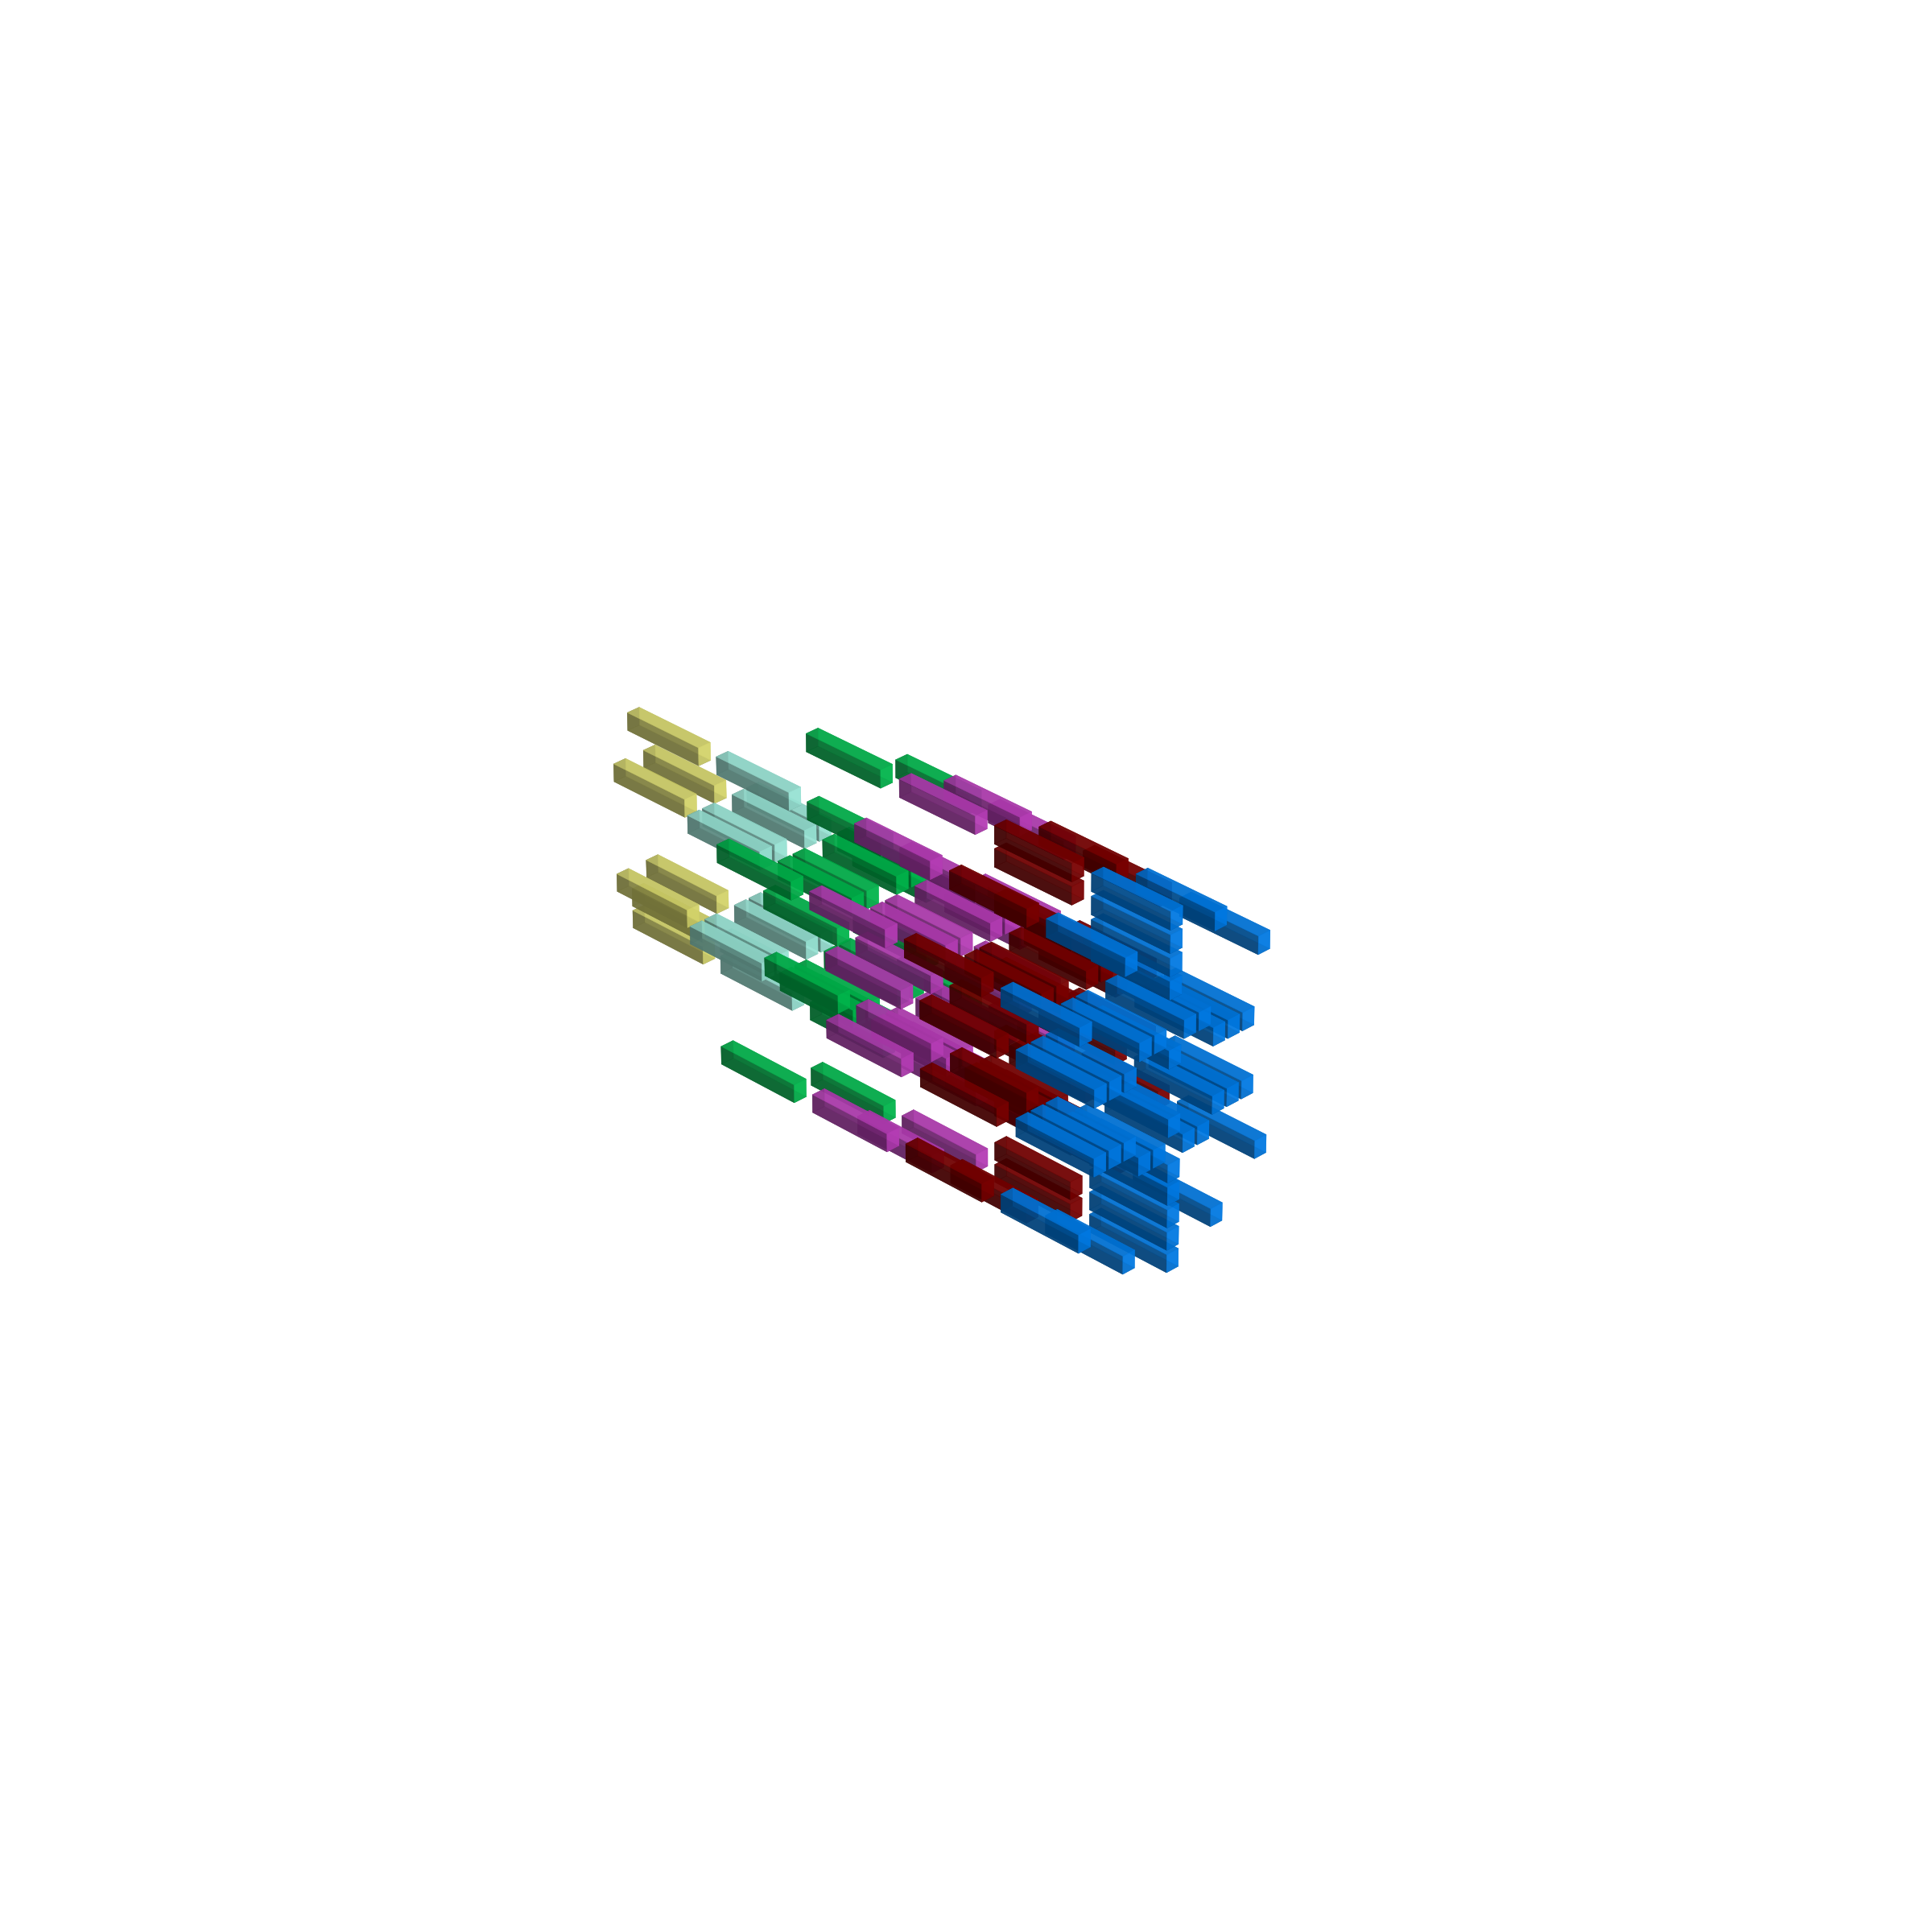
\includegraphics[width=8cm]{src/symmetries/pattern9_3-45.png}\\
        \vspace*{-8cm}
        \hspace*{1cm}
        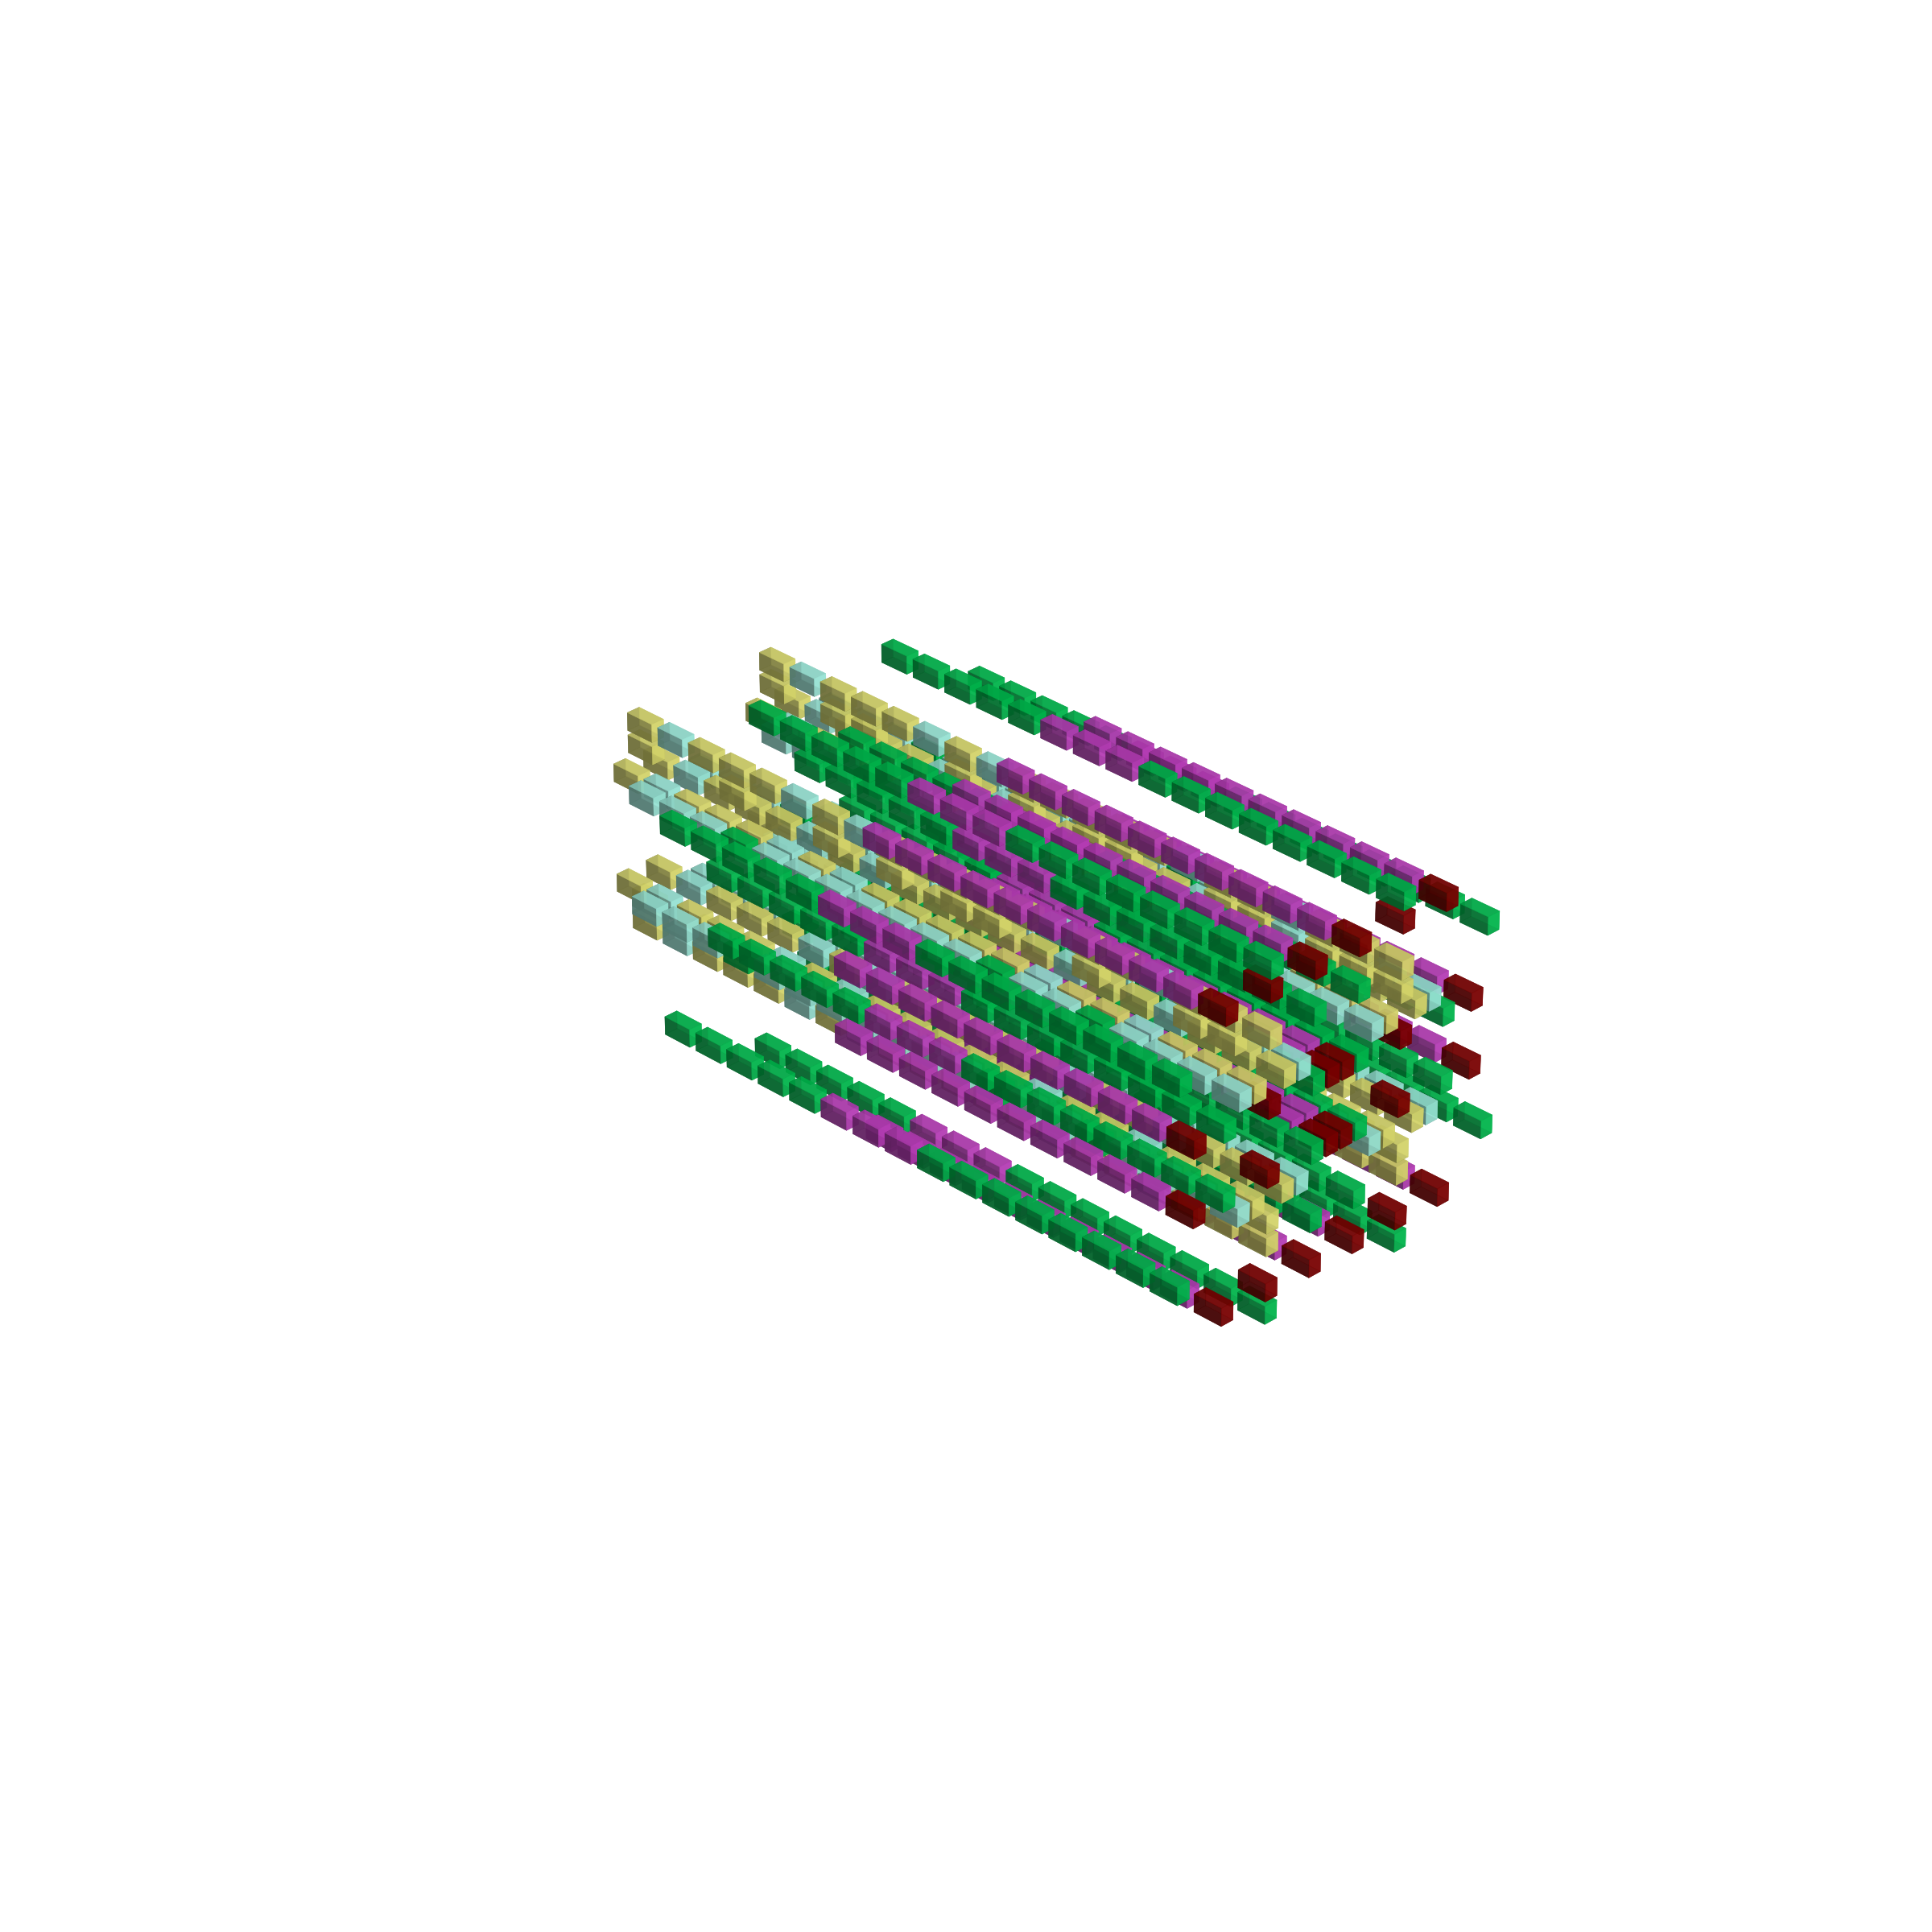
\includegraphics[width=8cm]{src/symmetries/pattern9_4-45.png}
        \vspace*{-2.5cm}
  \caption*{\getItem{9}}
  \end{figure}
\end{minipage}

\clearpage
\textbf{Lines 368-409. \icode{\textbf{PaintPixelForCurrentSymmetry\index{PaintPixelForCurrentSymmetry}}}}
\begin{lstlisting}[escapechar=\%]
;-------------------------------------------------------
; PaintPixelForCurrentSymmetry%\index{PaintPixelForCurrentSymmetry}%
;-------------------------------------------------------
PaintPixelForCurrentSymmetry%\index{PaintPixelForCurrentSymmetry}%   
        ; First paint the normal pattern without any
        ; symmetry.
        LDA pixelXPosition%\index{pixelXPosition}%
        PHA 
        LDA pixelYPosition%\index{pixelYPosition}%
        PHA 
        JSR PaintPixel%\index{PaintPixel}%

        LDA currentSymmetrySettingForStep%\index{currentSymmetrySettingForStep}%
        BNE HasSymmetry

CleanUpAndReturnFromSymmetry   
        PLA 
        STA pixelYPosition%\index{pixelYPosition}%
        PLA 
        STA pixelXPosition%\index{pixelXPosition}%
        RTS 

        RTS

HasSymmetry   
        CMP #X_AXIS_SYMMETRY
        BEQ XAxisSymmetry

        ; Has a pattern to paint on the Y axis
        ; symmetry so prepare for that.
        LDA #$27
        SEC 
        SBC pixelXPosition%\index{pixelXPosition}%
        STA pixelXPosition%\index{pixelXPosition}%

        ; If it has X_Y_SYMMETRY then we just 
        ; need to paint that, and we're done.
        LDY currentSymmetrySettingForStep%\index{currentSymmetrySettingForStep}%
        CPY #X_Y_SYMMETRY
        BEQ XYSymmetry

        ; If we're here it's either Y_AXIS_SYMMETRY
        ; or QUAD_SYMMETRY so we can paint a pattern
        ; on the Y axis.
        JSR PaintPixel%\index{PaintPixel}%

\end{lstlisting}
\clearpage

\rhead[]{\icode{PaintPixelForCurrentSymmetry\index{PaintPixelForCurrentSymmetry}}}
\textbf{Lines 368-409. \icode{\textbf{PaintPixelForCurrentSymmetry\index{PaintPixelForCurrentSymmetry}}}:} This routine seems a lot more convoluted than it
ought to be. What it needs to do is figure out which of the four symmetries it ought to paint and then paint them. Clarity
is a victim of optimization in this instance - making the routine as compact as possible means we need to pick through it
to understand it.

\textbf{Lines 372,374. \icode{\textbf{PHA}}:} Notice that we're pushing the values in \icode{pixelXPosition\index{pixelXPosition}} and \icode{pixelYPosition\index{pixelYPosition}}
on to the stack. The reason for this is that we may have to modify one or both of \icode{pixelXPosition\index{pixelXPosition}/pixelYPosition\index{pixelYPosition}} when
painting the symmetries, so pushing them onto the stack here means we can later pull them back off the stack (\icode{PLA}) and restore each to their original
values when we're finished.

\textbf{Lines 380-387. \icode{\textbf{CleanUpAndReturnFromSymmetry}}:} The simplest case is easiest. If we get to here
the symmetry setting just requires one pattern to be drawn (\icode{NO SYMMETRY}) so after calling \icode{PaintPixel\index{PaintPixel}}
we can return early.

\textbf{Lines 389-409. \icode{\textbf{HasSymmetry}}:} We know what this section ought to be doing, but you really do have
to stare at it quite a long time to work out how it's doing it. What it ought to be doing is painting a pixel reflected on one or more
of the X and Y axes depending on the setting of \icode{currentSymmetrySettingForStep\index{currentSymmetrySettingForStep}}. In the process it jumps around a bit,
shuffles values on and off the stack and has a couple of points where the routine can return early. None of this really aids
the cause of understanding. We'll pick the second simplest case to help give you an idea of how the routine works. This is where
the \icode{X\_AXIS\_SYMMETRY} is active so the code branches to \icode{XAxisSymmetry}.
It's called \icode{X-AXIS SYMMETRY} but the reflection is on the Y Axis, i.e.
on the vertical. Maybe it's called that because the patterns share the same X-coordinate? Either way, it's a confusing name for what
it is.

\begin{figure}[H]
    \centering
      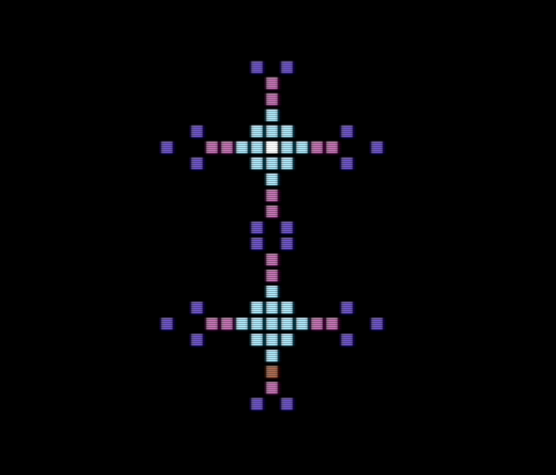
\includegraphics[height=5cm]{src/symmetries/xaxis.png}
  \caption*{\icode{X-AXIS SYMMETRY} - despite the name it's along the Y axis.}
\end{figure}

\clearpage
\textbf{Lines 409-458. \icode{\textbf{PaintPixelForCurrentSymmetry\index{PaintPixelForCurrentSymmetry}} continued.}}
\begin{lstlisting}[escapechar=\%]
        ; If it's Y_AXIS_SYMMETRY we're done and can 
        ; return.
        LDA currentSymmetrySettingForStep%\index{currentSymmetrySettingForStep}%
        CMP #Y_AXIS_SYMMETRY
        BEQ CleanUpAndReturnFromSymmetry

        ; Has QUAD_SYMMETRY so the remaining steps are
        ; to paint two more: one on our X axis and one
        ; on our Y axis.

        ; First we do the Y axis.
        LDA #NUM_ROWS
        SEC 
        SBC pixelYPosition%\index{pixelYPosition}%
        STA pixelYPosition%\index{pixelYPosition}%
        JSR PaintPixel%\index{PaintPixel}%

        ; Paint one on the X axis.
PaintXAxisPixelForSymmetry    
        PLA 
        TAY 
        PLA 
        STA pixelXPosition%\index{pixelXPosition}%
        TYA 
        PHA 
        JSR PaintPixel%\index{PaintPixel}%
        PLA 
        STA pixelYPosition%\index{pixelYPosition}%
        RTS 

XAxisSymmetry   
        LDA #NUM_ROWS
        SEC 
        SBC pixelYPosition%\index{pixelYPosition}%
        STA pixelYPosition%\index{pixelYPosition}%
        JMP PaintXAxisPixelForSymmetry

XYSymmetry   
        LDA #NUM_ROWS
        SEC 
        SBC pixelYPosition%\index{pixelYPosition}%
        STA pixelYPosition%\index{pixelYPosition}%
        JSR PaintPixel%\index{PaintPixel}%
        PLA 
        STA pixelYPosition%\index{pixelYPosition}%
        PLA 
        STA pixelXPosition%\index{pixelXPosition}%
        RTS 
\end{lstlisting}
\clearpage

\rhead[]{\icode{PaintXAxisPixelForSymmetry} cont.}
\textbf{Lines 441-446. \icode{\textbf{XAxisSymmetry}}:} So what we actually want to do here is reflect the pattern on the Y axis. This means manipulating \icode{pixelYPosition\index{pixelYPosition}} so that it's
offset halfway down the screen.  The easiest way to do this is to subtract our current Y position from the total height of the screen.
We do this by loading the height (\icode{NUM\_ROWS}) into the \icode{Accumulator} and substracting our Y position from it 
(\icode{SBC pixelYPosition\index{pixelYPosition}} - we then update our Y position with the new value (\icode{STA pixelYPosition\index{pixelYPosition}}). Next we jump to
\icode{PaintXAxisPixelForSymmetry}.

\textbf{Lines 429-439. \icode{\textbf{PaintXAxisPixelForSymmetry}}:} Now we can update our X position. We do this by retrieving it
from the stack, where we stowed it at the top of \icode{PaintPixelForCurrentSymmetry\index{PaintPixelForCurrentSymmetry}} and in case we previously modified it elsewhere in the routine. 
Because we pushed the X position first, and the Y position after it, the first item we pull from the stack will be the Y position.
So we pull and stow it in the \icode{Y} register:

\begin{lstlisting}[escapechar=\%]
PaintXAxisPixelForSymmetry    
        PLA 
        TAY 
\end{lstlisting}

Now we can pull the X position:
\begin{lstlisting}[escapechar=\%]
        PLA 
        STA pixelXPosition%\index{pixelXPosition}%
\end{lstlisting}

And then push the Y position back onto the stack again:
\begin{lstlisting}[escapechar=\%]
        TYA 
        PHA 
\end{lstlisting}

After calling \icode{PaintPixel\index{PaintPixel}} we pull the Y position off the stack again and reload it to \icode{pixelYPosition\index{pixelYPosition}} so that we leave
the routine with both \icode{pixelXPosition\index{pixelXPosition}/pixelYPosition\index{pixelYPosition}} by any of the monkey business we got up to in \icode{PaintPixel\index{PaintPixel}}.

\begin{lstlisting}[escapechar=\%]
        JSR PaintPixel%\index{PaintPixel}%
        PLA 
        STA pixelYPosition%\index{pixelYPosition}%
        RTS 
\end{lstlisting}

\clearpage
\rhead[]{\leftmark}

\clearpage
\textbf{Lines 518-526. \icode{\textbf{symmetrySettingForStepCount\index{symmetrySettingForStepCount}}}}
\begin{lstlisting}[escapechar=\%]
symmetrySettingForStepCount%\index{symmetrySettingForStepCount}%
        .BYTE $FF,$FF,$FF,$FF,$FF,$FF,$FF,$FF
        .BYTE $FF,$FF,$FF,$FF,$FF,$FF,$FF,$FF
        .BYTE $FF,$FF,$FF,$FF,$FF,$FF,$FF,$FF
        .BYTE $FF,$FF,$FF,$FF,$FF,$FF,$FF,$FF
        .BYTE $FF,$FF,$FF,$FF,$FF,$FF,$FF,$FF
        .BYTE $FF,$FF,$FF,$FF,$FF,$FF,$FF,$FF
        .BYTE $FF,$FF,$FF,$FF,$FF,$FF,$FF,$FF
        .BYTE $FF,$FF,$FF,$FF,$FF,$FF,$FF,$FF
\end{lstlisting}
\textbf{Lines 644-668. \icode{\textbf{ShouldDoAPaint}}}
\begin{lstlisting}[escapechar=\%]
ShouldDoAPaint   
        ...
        ; Get the x and y positions for this pixel.
        ; X is currentIndexToPixelBuffers%\index{currentIndexToPixelBuffers}%
        LDA pixelXPositionArray%\index{pixelXPositionArray}%,X
        STA pixelXPosition%\index{pixelXPosition}%
        LDA pixelYPositionArray%\index{pixelYPositionArray}%,X
        STA pixelYPosition%\index{pixelYPosition}%

        LDA patternIndexArray%\index{patternIndexArray}%,X
        STA patternIndex%\index{patternIndex}%

        LDA symmetrySettingForStepCount%\index{symmetrySettingForStepCount}%,X
        STA currentSymmetrySettingForStep%\index{currentSymmetrySettingForStep}%
\end{lstlisting}
\rhead[]{\icode{symmetrySettingForStepCount\index{symmetrySettingForStepCount}}}
\clearpage

\textbf{Lines 518-526. \icode{\textbf{symmetrySettingForStepCount\index{symmetrySettingForStepCount}}}:} You probably didn't notice that in \icode{PaintPixelForCurrentSymmetry\index{PaintPixelForCurrentSymmetry}}
we inspected the current symmetry setting in a variable called \icode{currentSymmetrySettingForStep\index{currentSymmetrySettingForStep}} rather than \icode{currentSymmetrySetting\index{currentSymmetrySetting}}.
Unlike in the listing version, where the symmetry setting was immutable, the user can change the setting at any time so that forces us to
manage a condition where different symmetries are in force at different stages in the display. For this reason we have an additional array
called \icode{symmetrySettingForStepCount\index{symmetrySettingForStepCount}} that tells us what the symmetry used for the current step is.  

\textbf{Lines 644-668. \icode{\textbf{ShouldDoAPaint}}:} Here we load the symmetry for the current step from our array and store it in
\icode{currentSymmetrySettingForStep\index{currentSymmetrySettingForStep}} for use later in \icode{PaintPixelForCurrentSymmetry\index{PaintPixelForCurrentSymmetry}}.

\clearpage
\hspace{-1cm}
\begin{minipage}[b]{0.50\linewidth}                                       
  \begin{figure}[H]
      \centering
        \vspace*{-1cm}
        \hspace*{-2cm}
        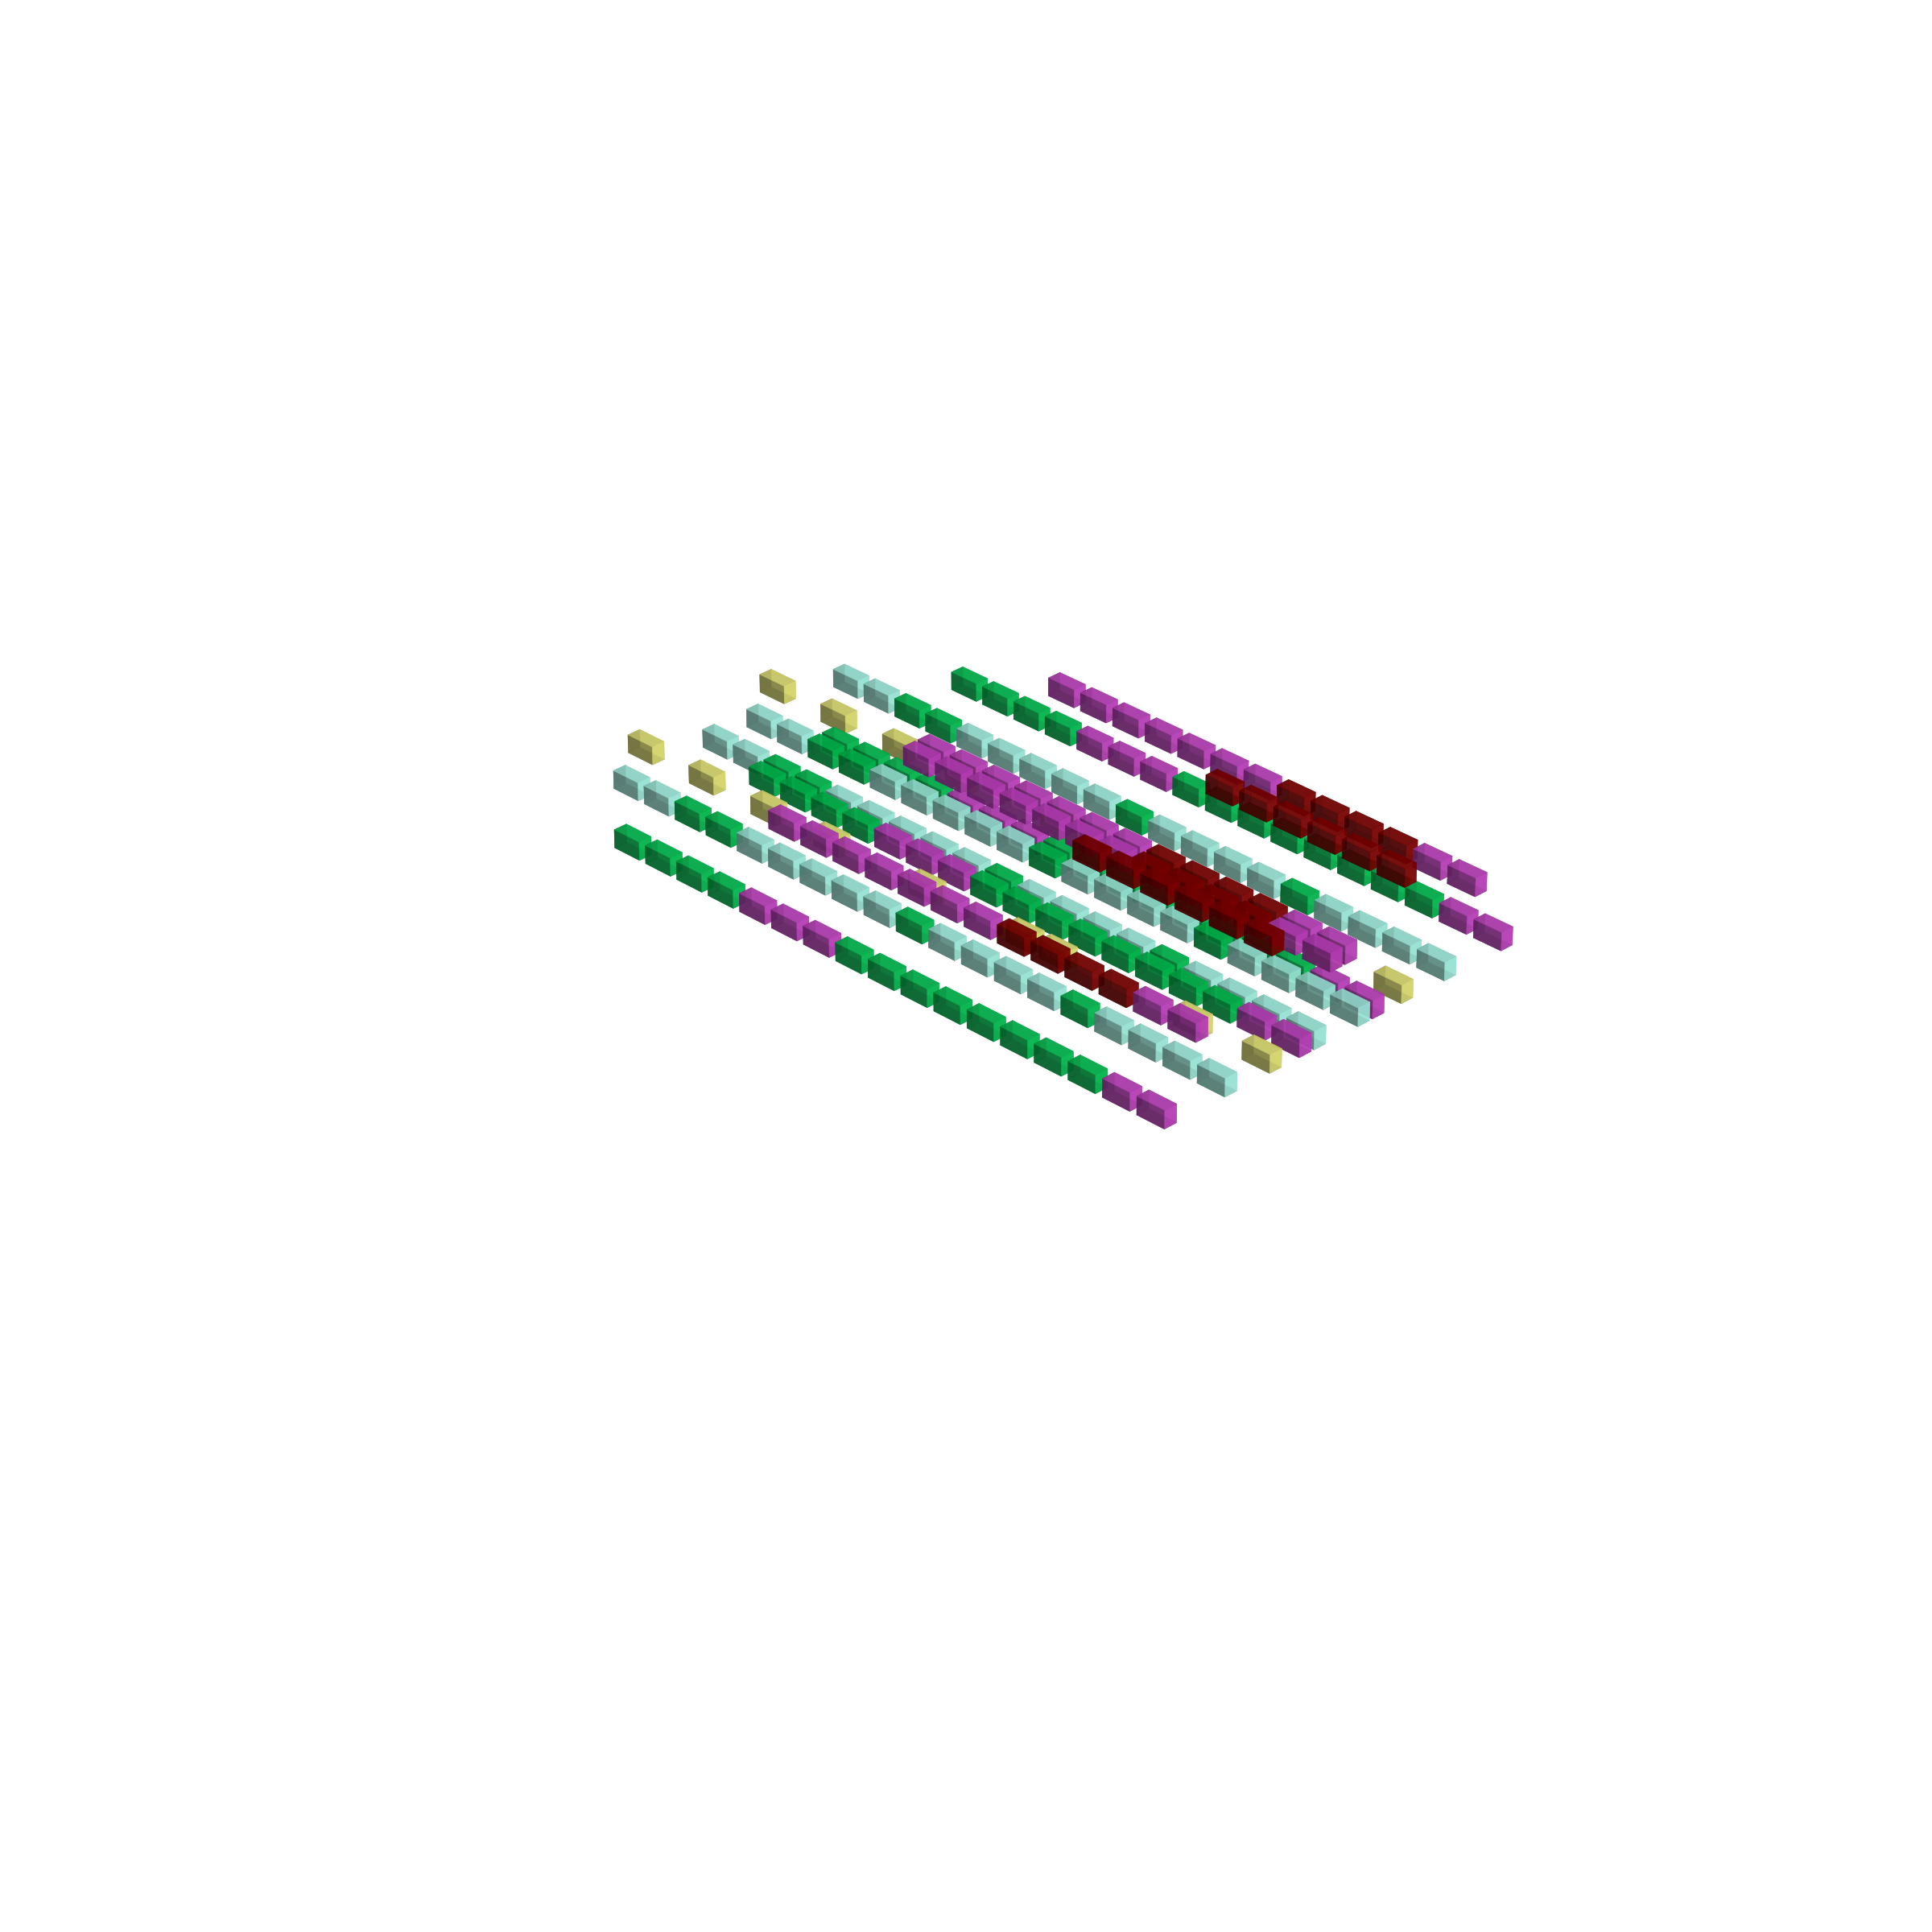
\includegraphics[width=8cm]{src/symmetries/pattern10_1-45.png}%
        \hspace*{-4cm}
        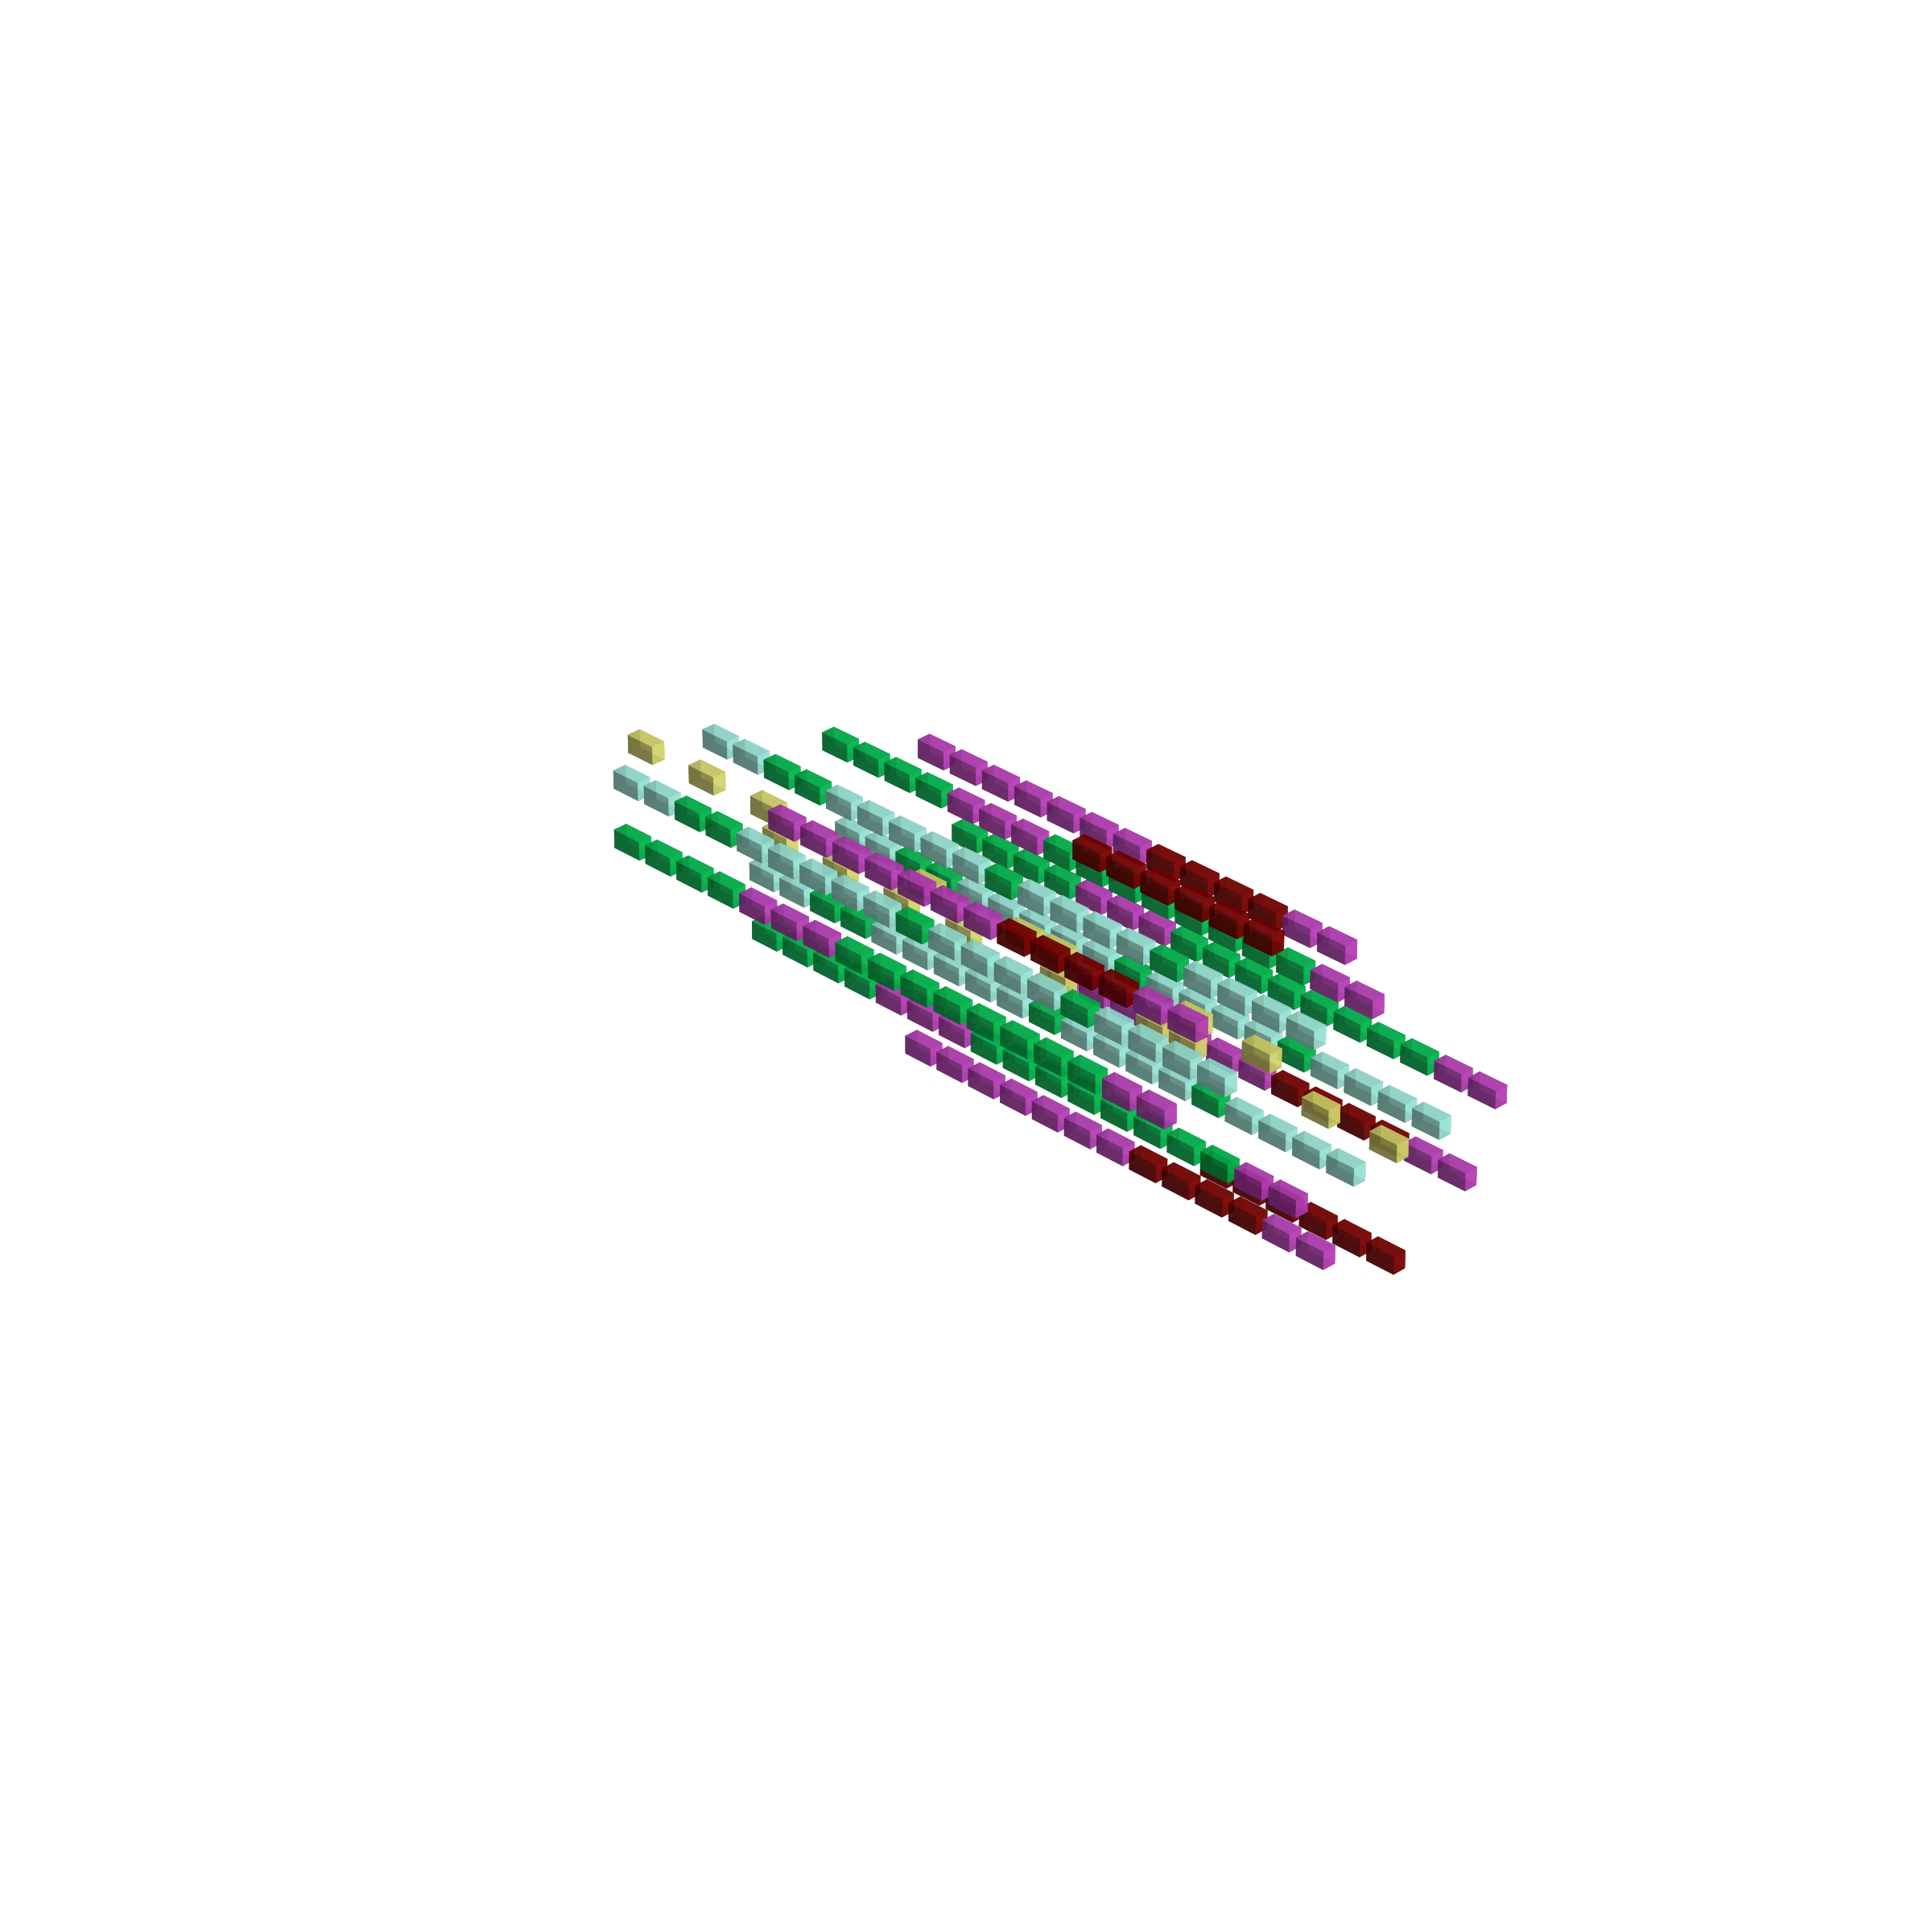
\includegraphics[width=8cm]{src/symmetries/pattern10_2-45.png}\\
        \vspace*{-5cm}
        \hspace*{-3cm}
        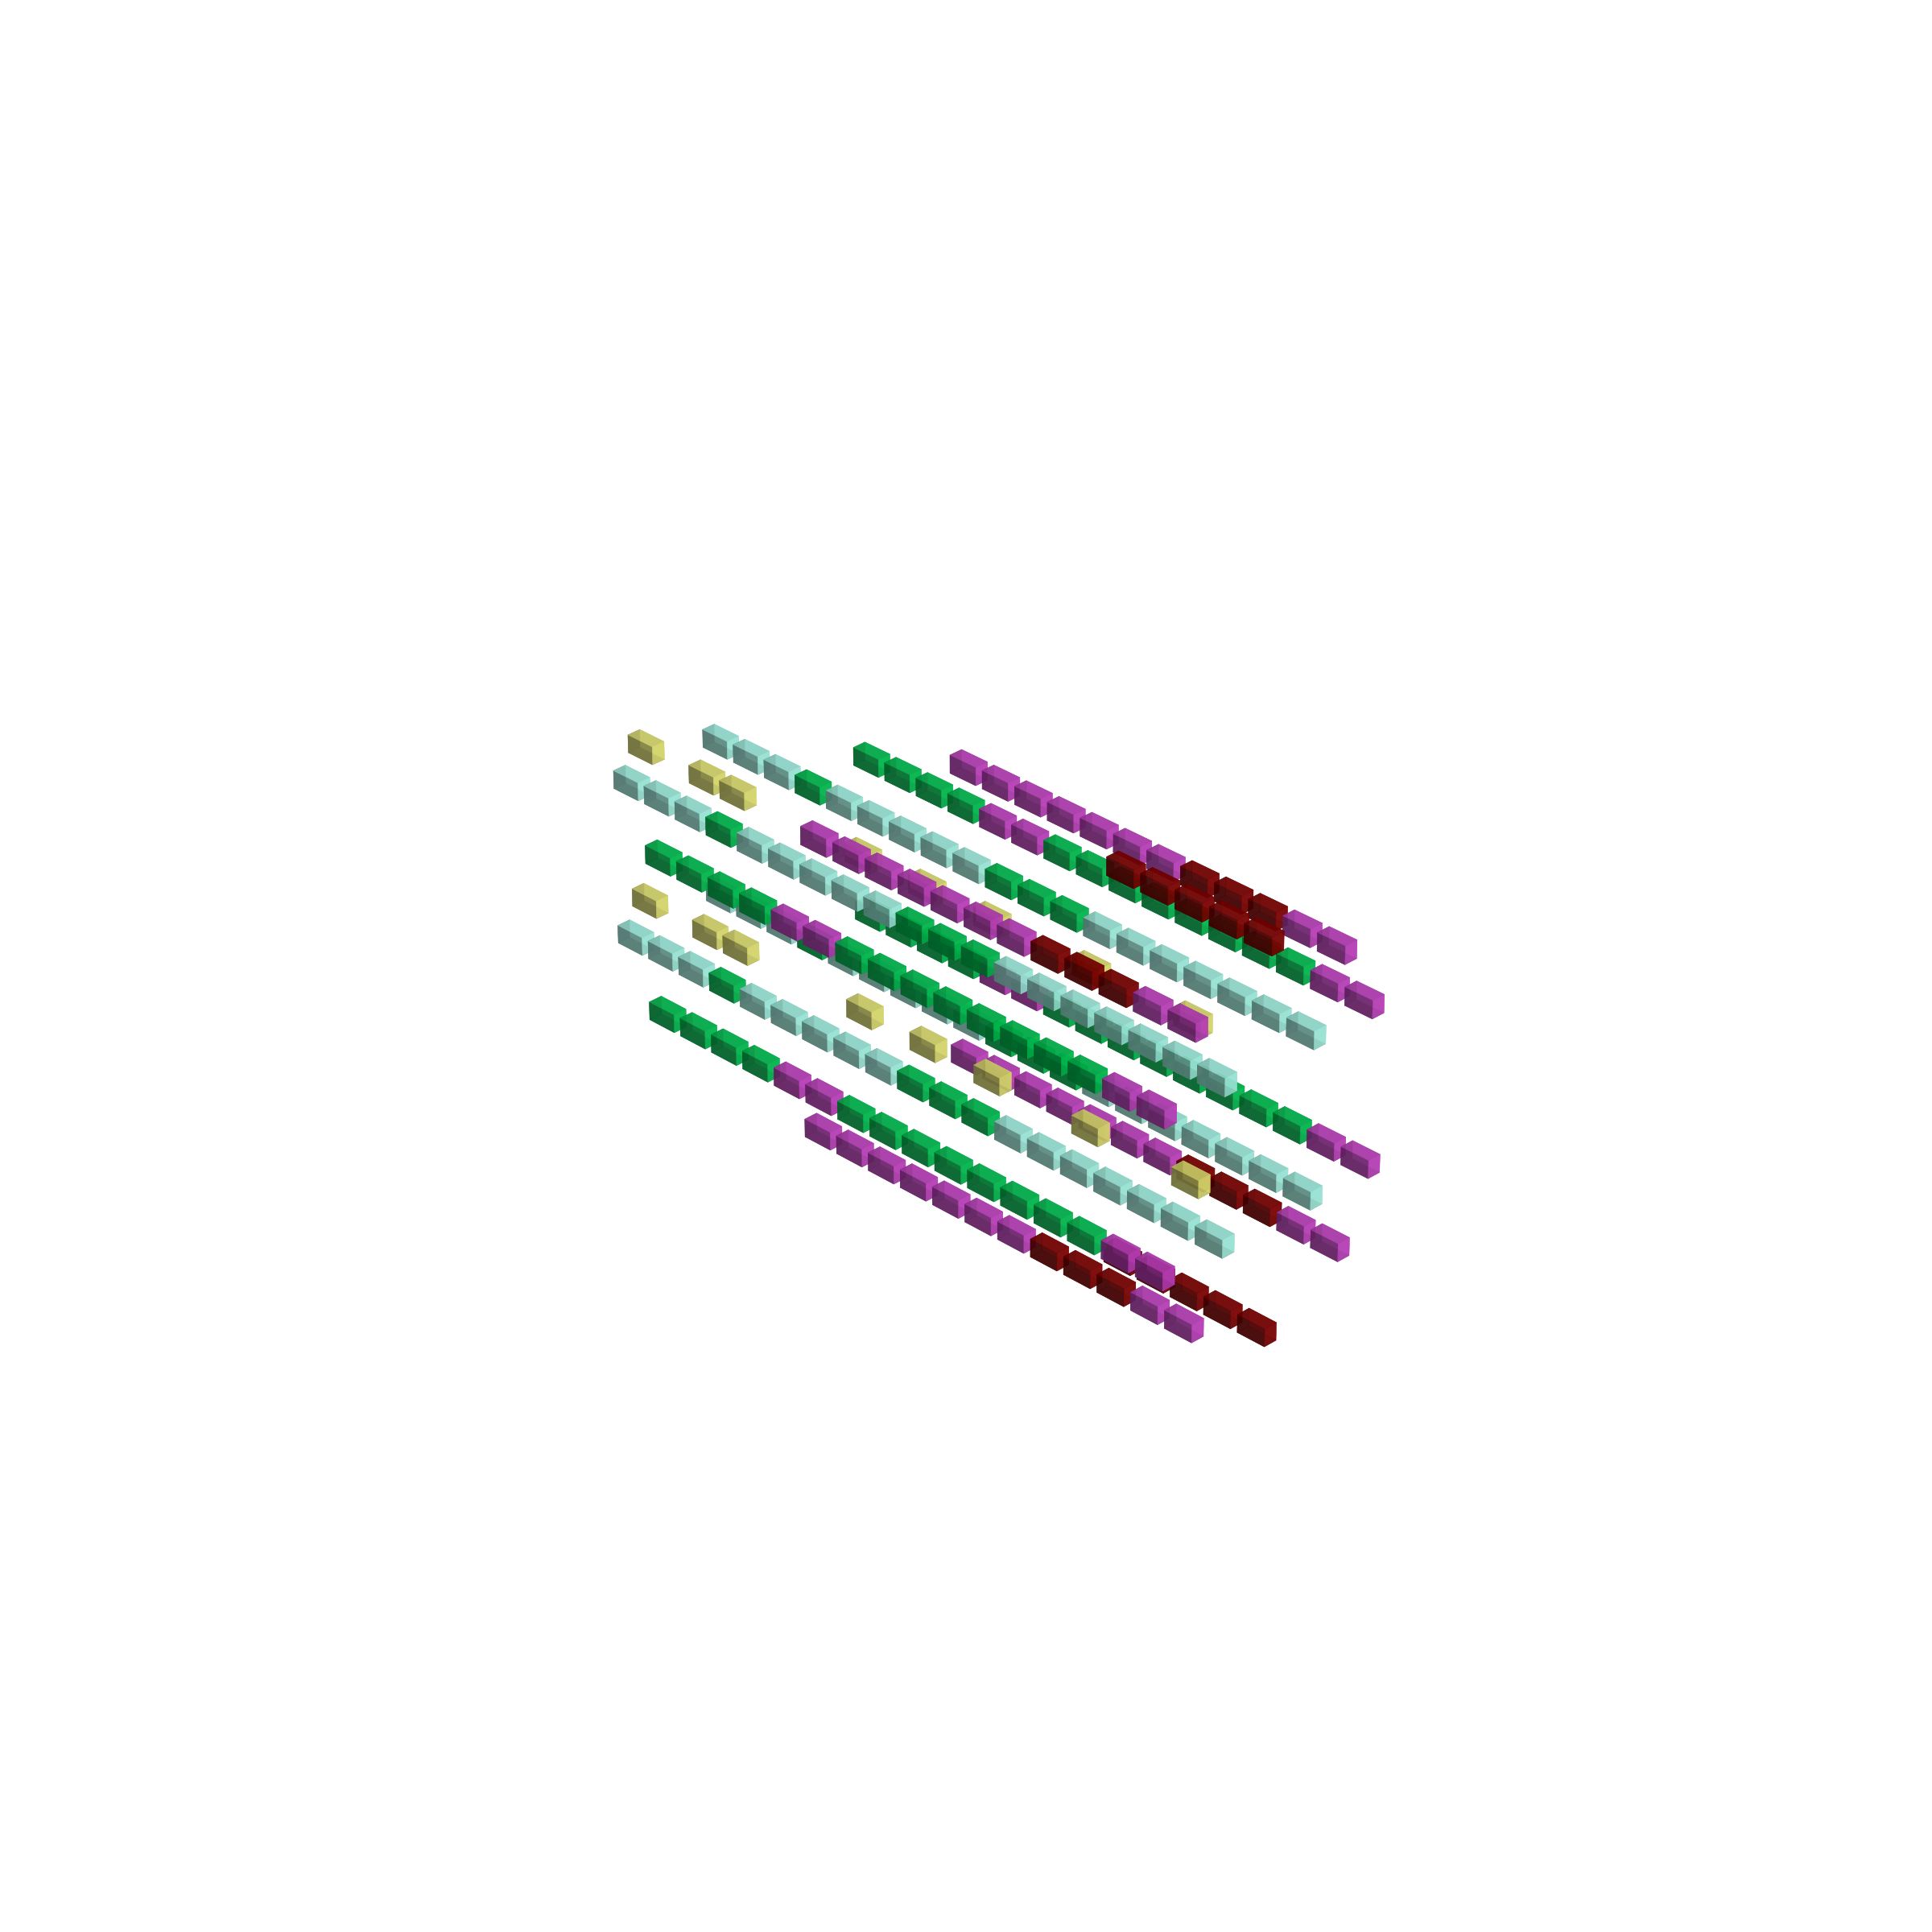
\includegraphics[width=8cm]{src/symmetries/pattern10_3-45.png}\\
        \vspace*{-8cm}
        \hspace*{2cm}
        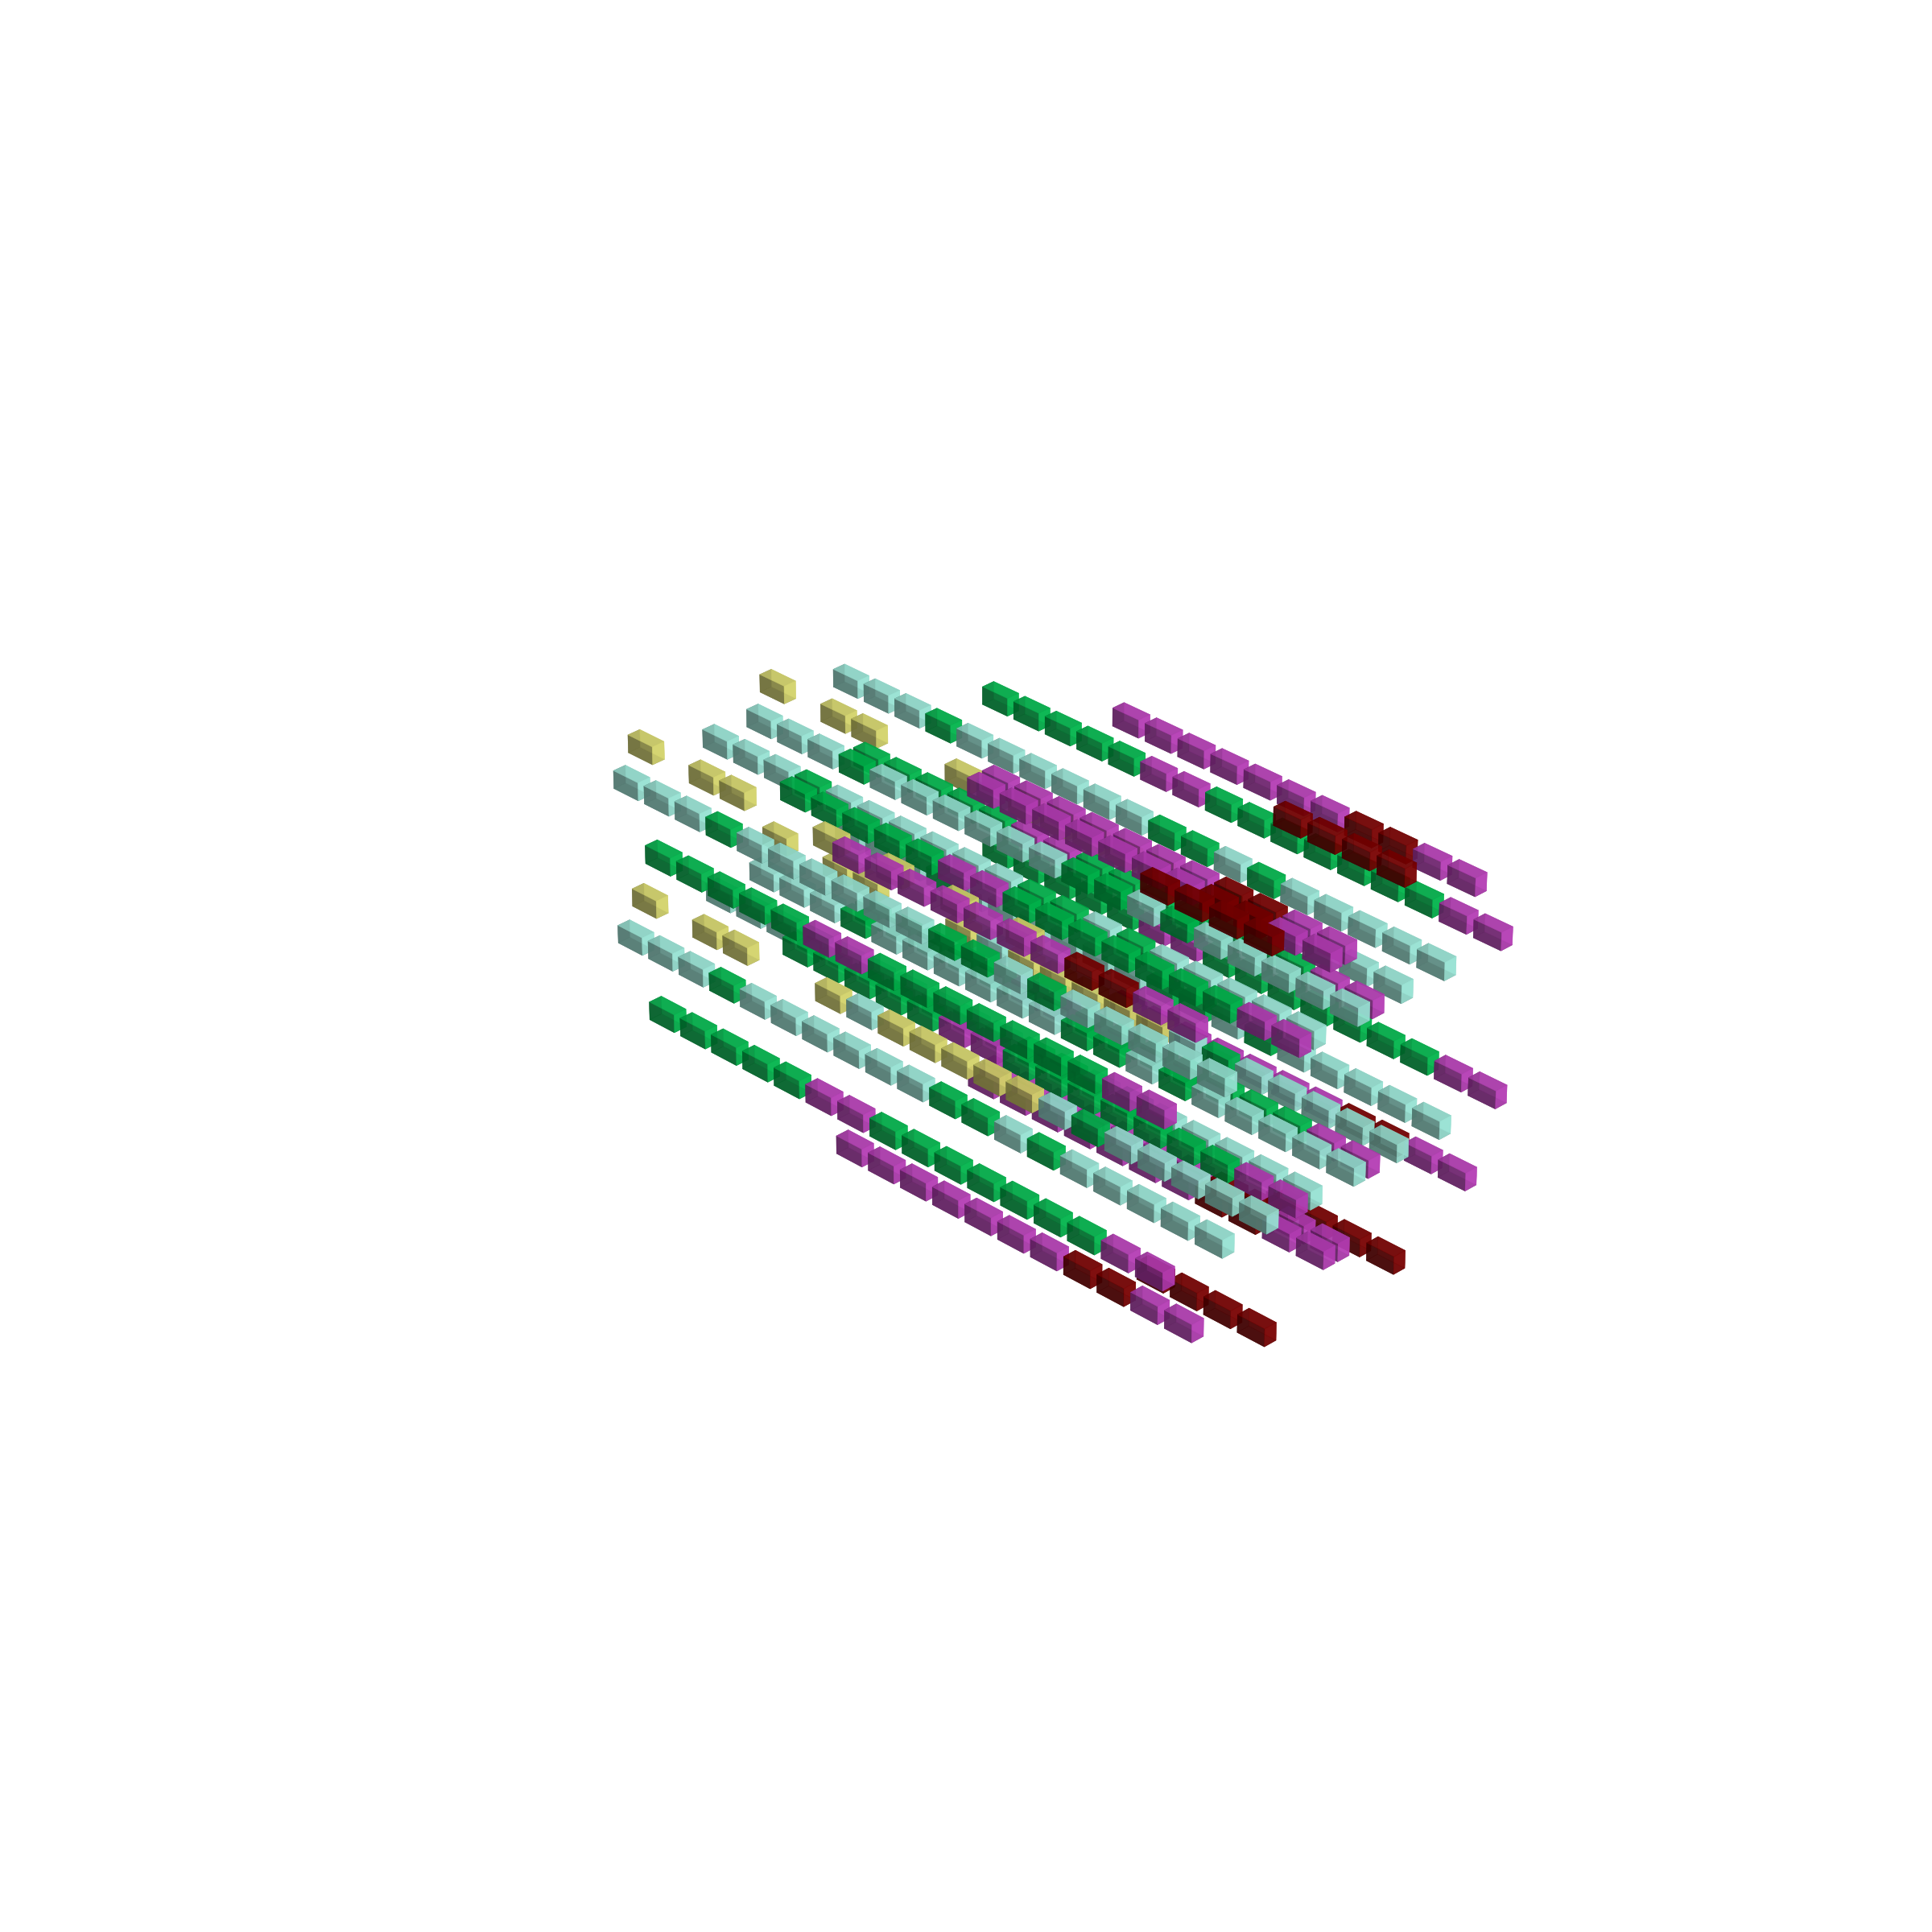
\includegraphics[width=8cm]{src/symmetries/pattern10_4-45.png}
        \vspace*{-2.5cm}
  \caption*{\getItem{10}}
  \end{figure}
\end{minipage}
\hspace{1cm}
\begin{minipage}[b]{0.50\linewidth}                                       
  \begin{figure}[H]
      \centering
        \vspace*{-1cm}
        \hspace*{-2cm}
        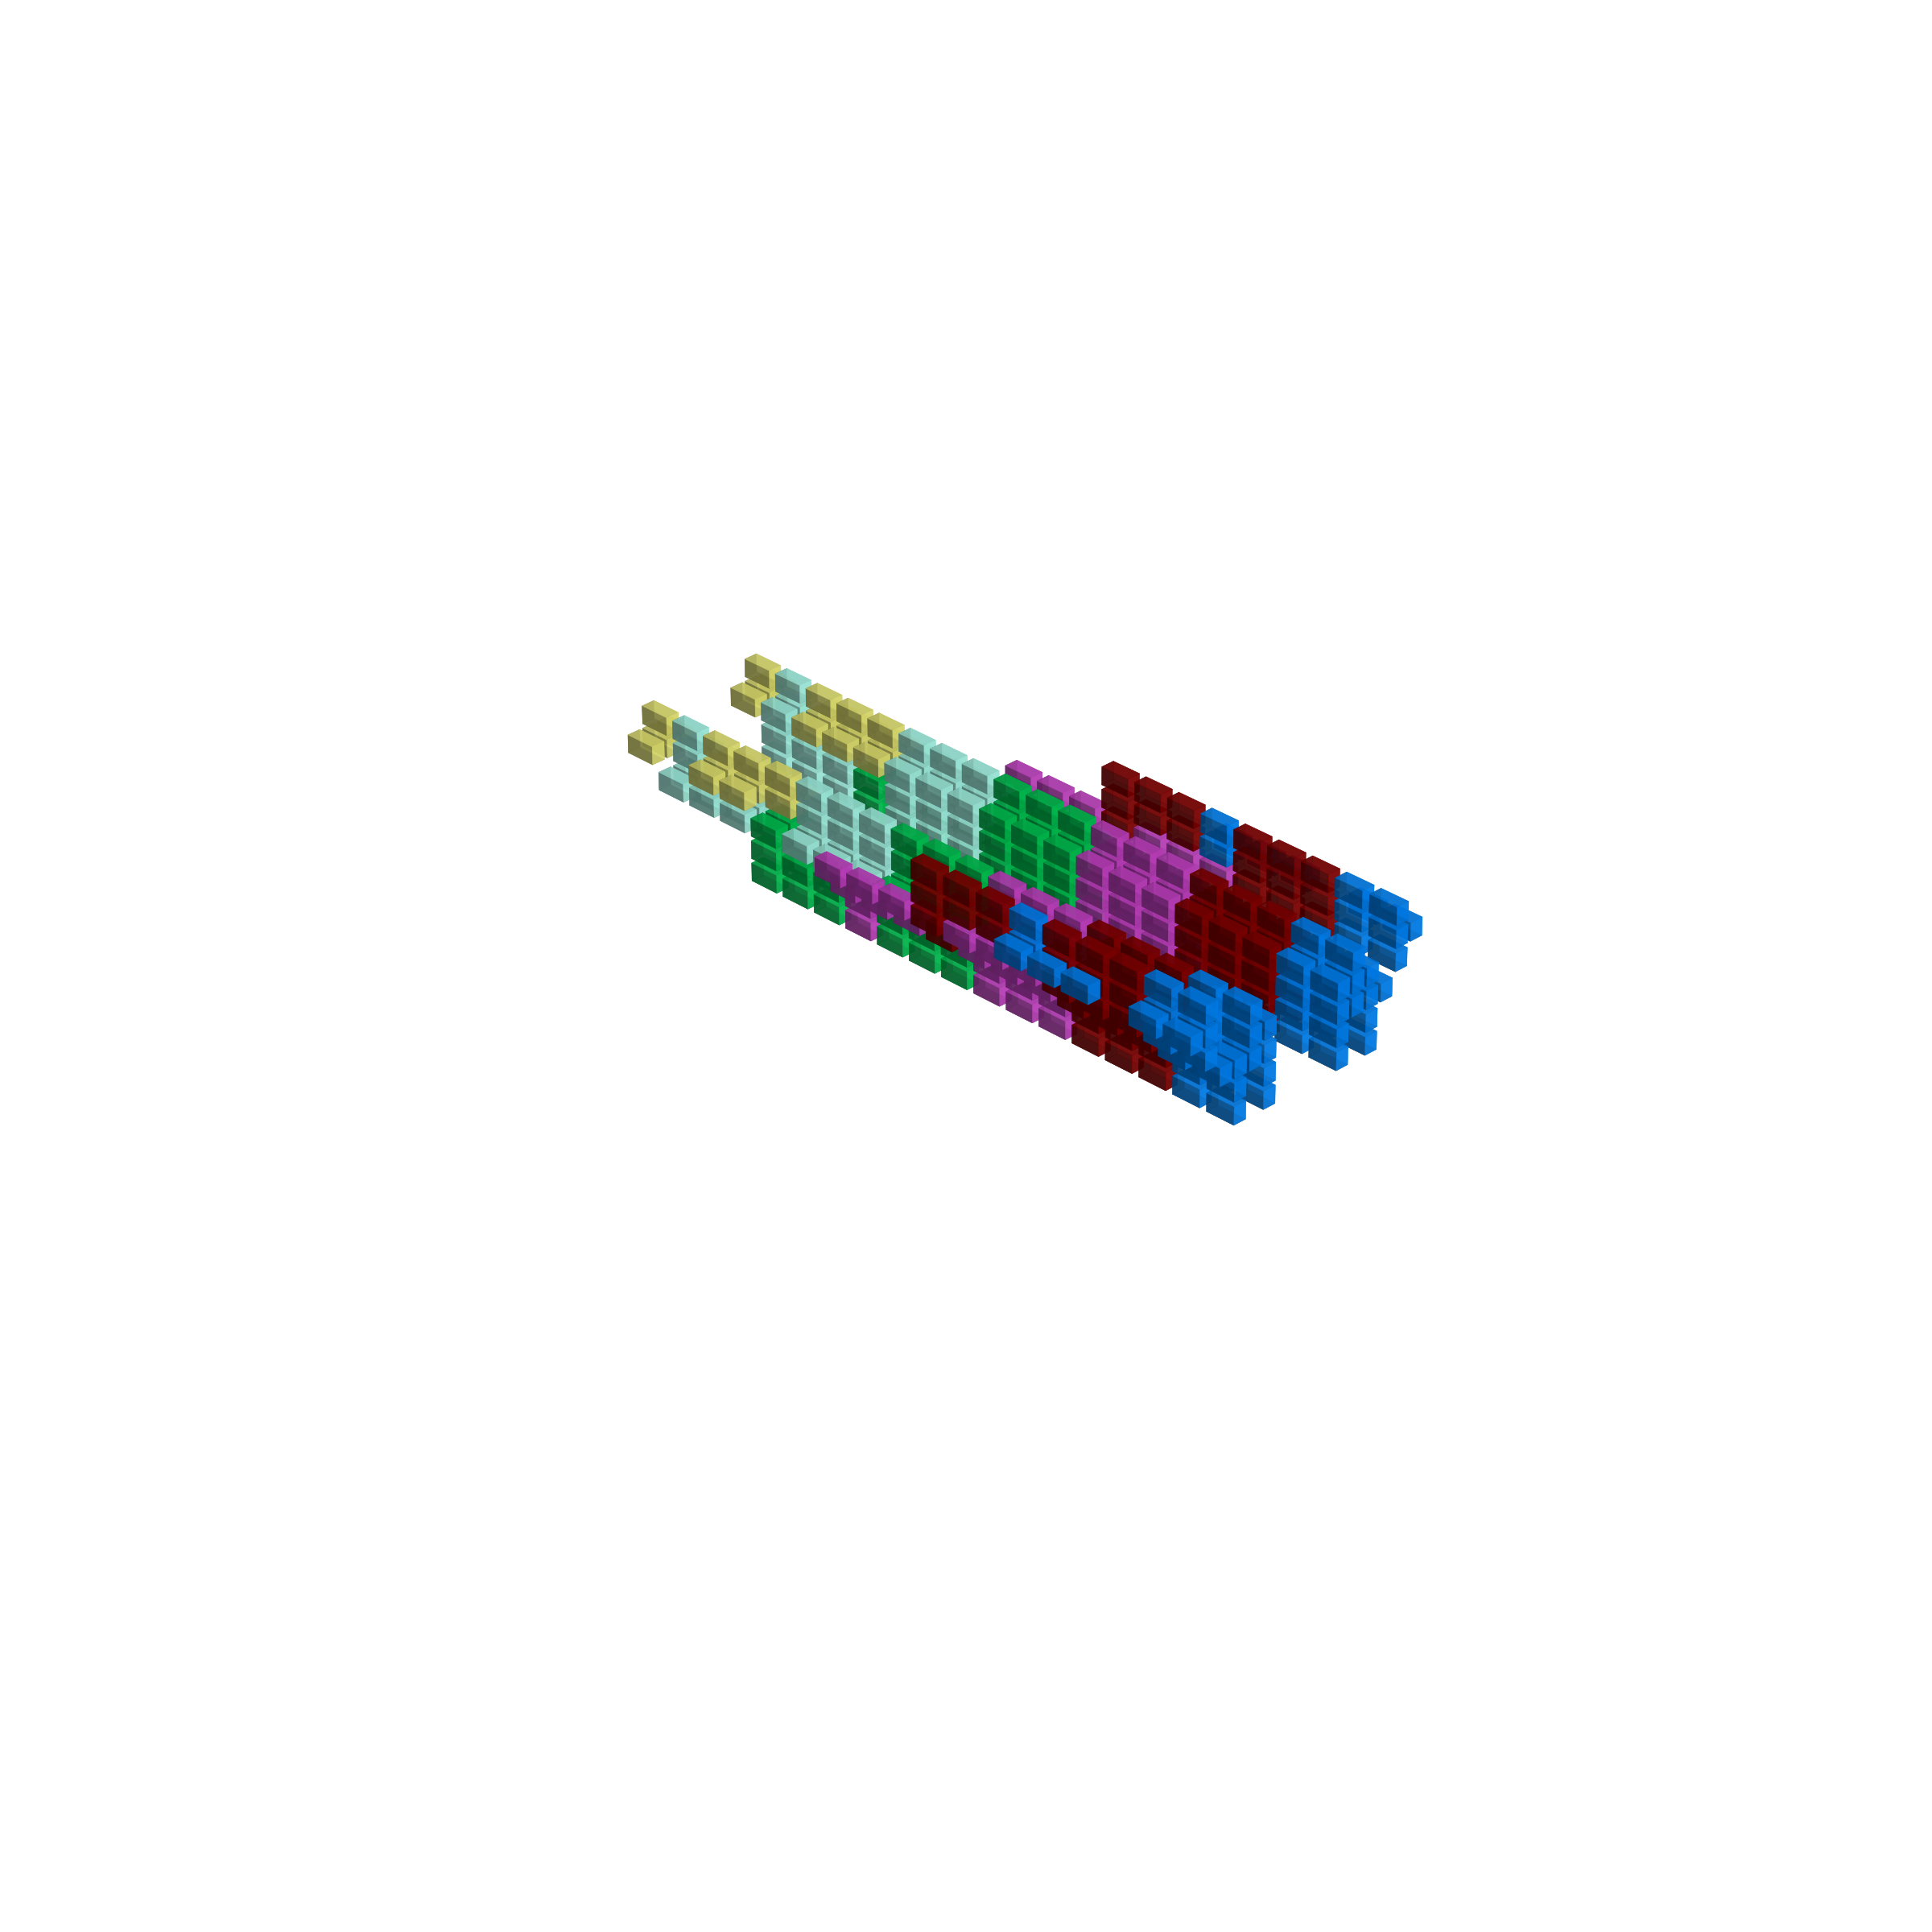
\includegraphics[width=8cm]{src/symmetries/pattern11_1-45.png}%
        \hspace*{-4cm}
        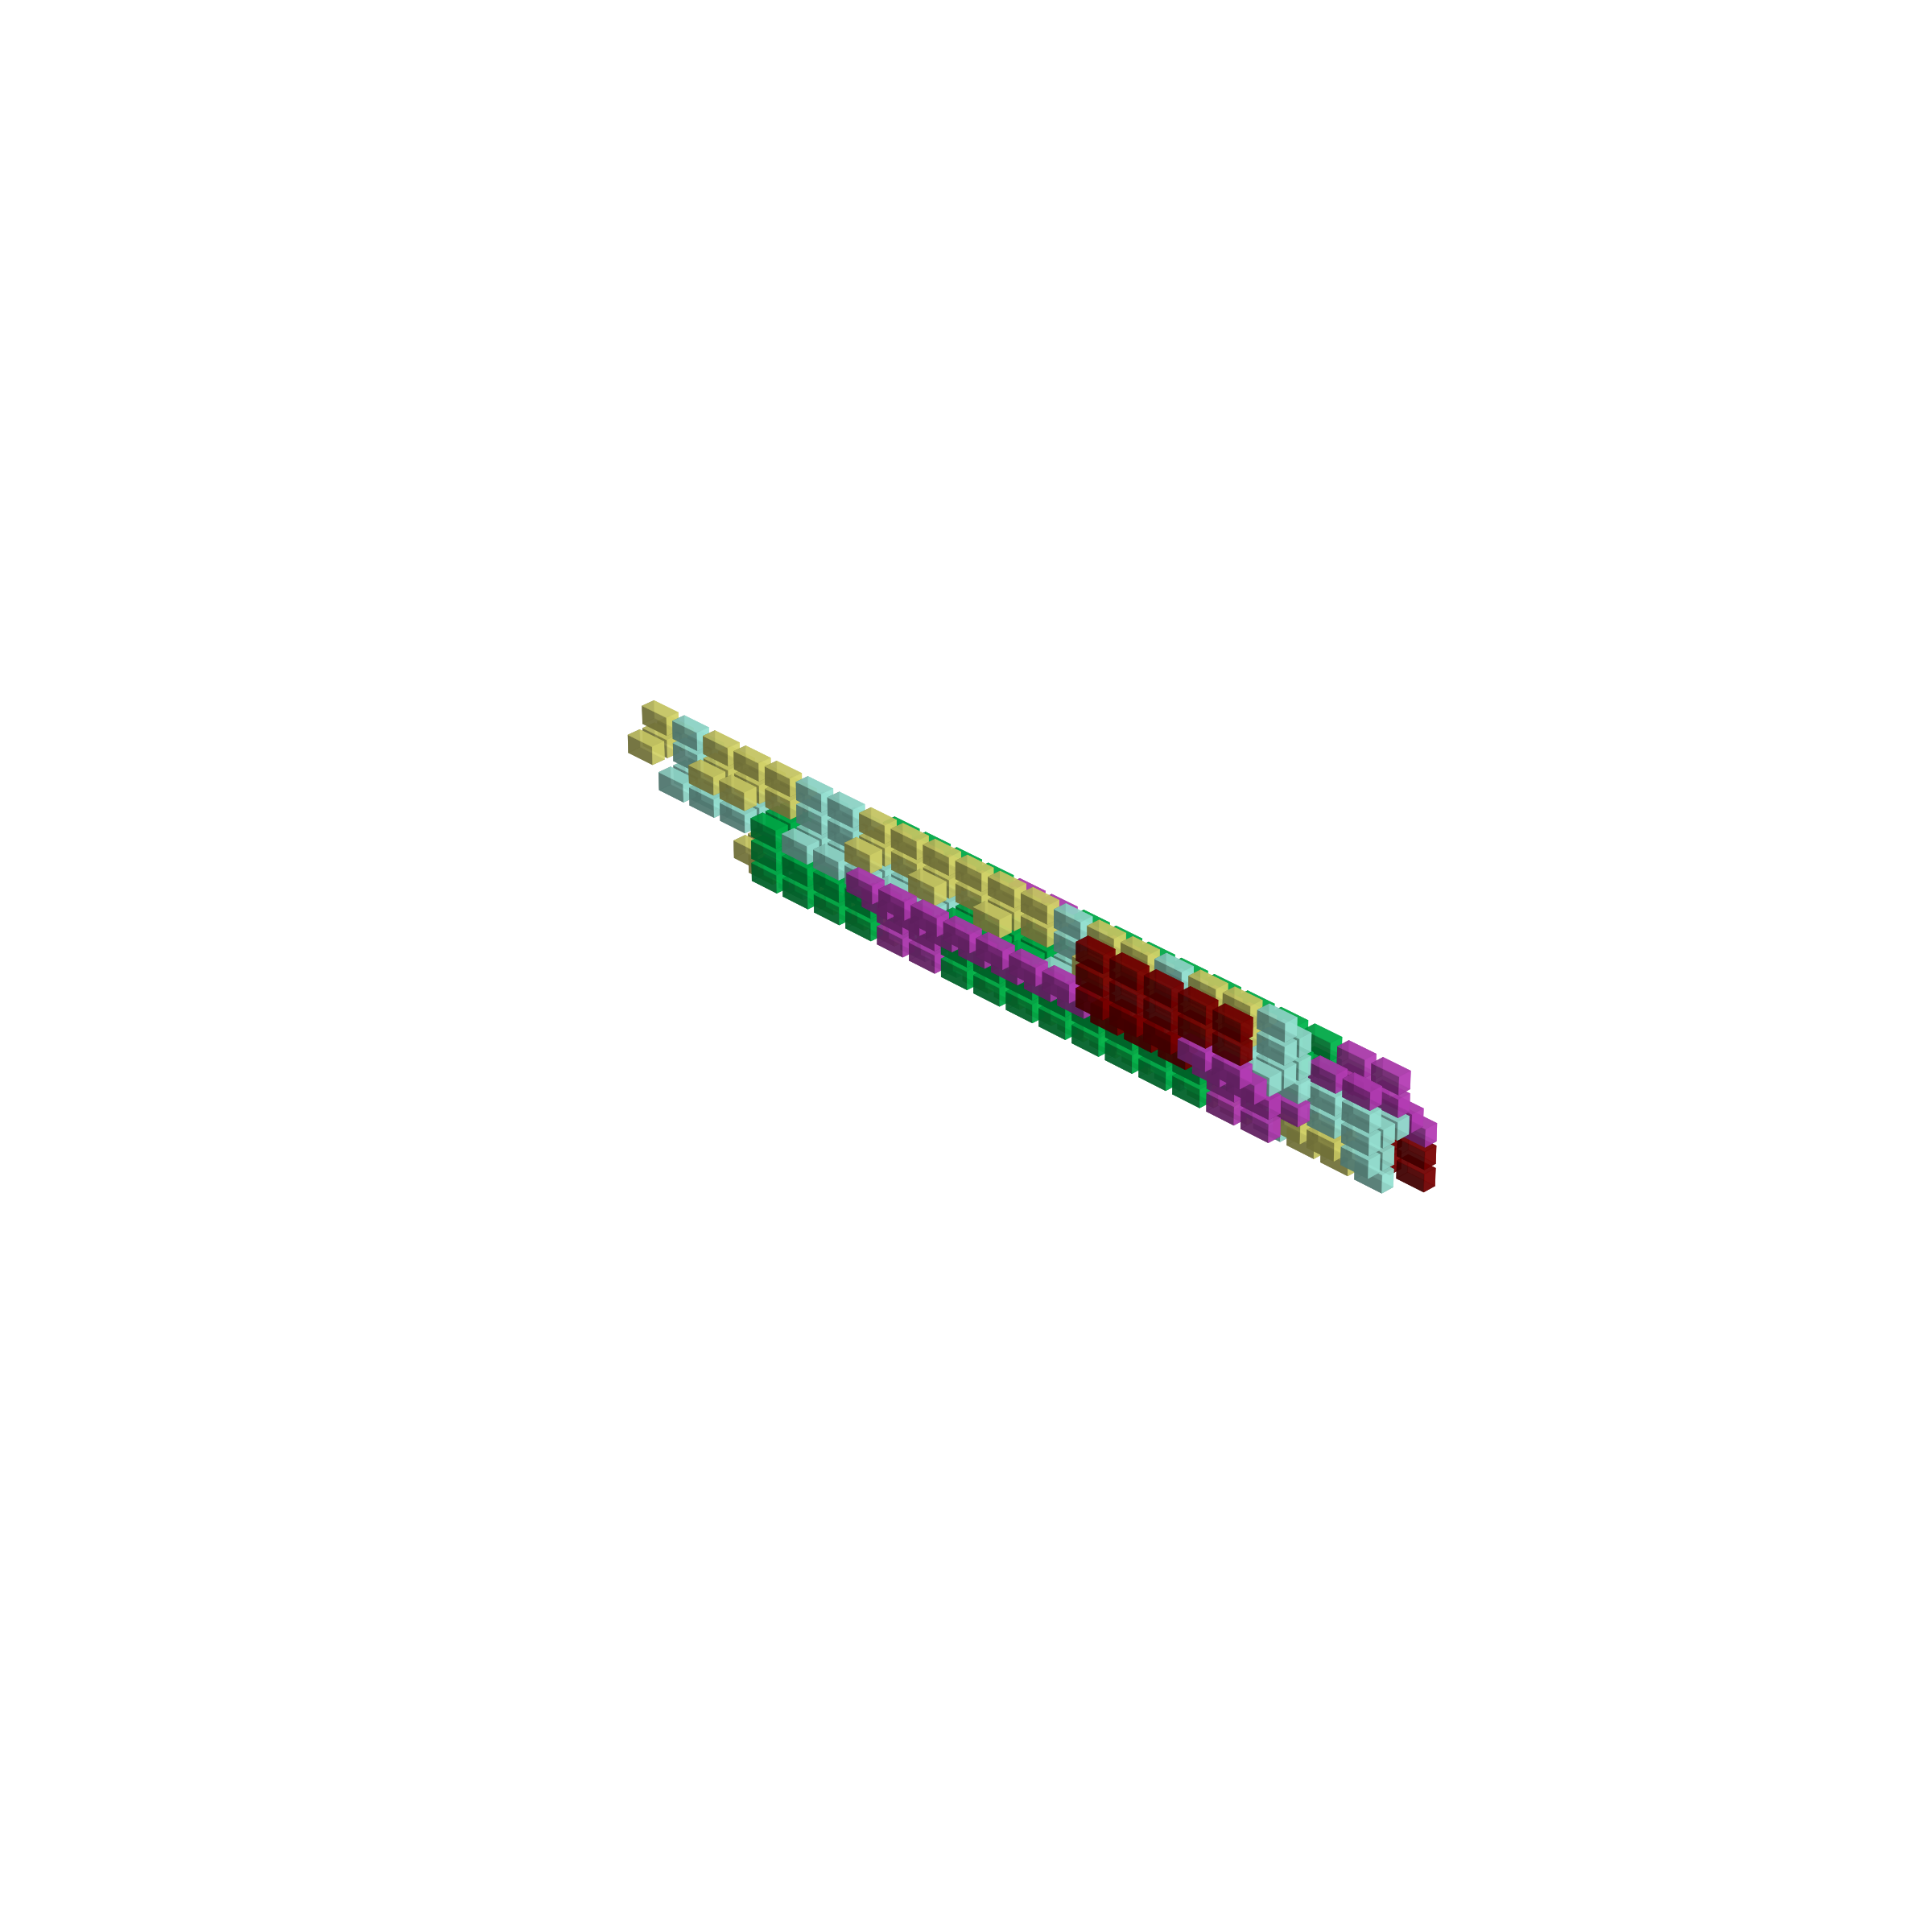
\includegraphics[width=8cm]{src/symmetries/pattern11_2-45.png}\\
        \vspace*{-5cm}
        \hspace*{-1cm}
        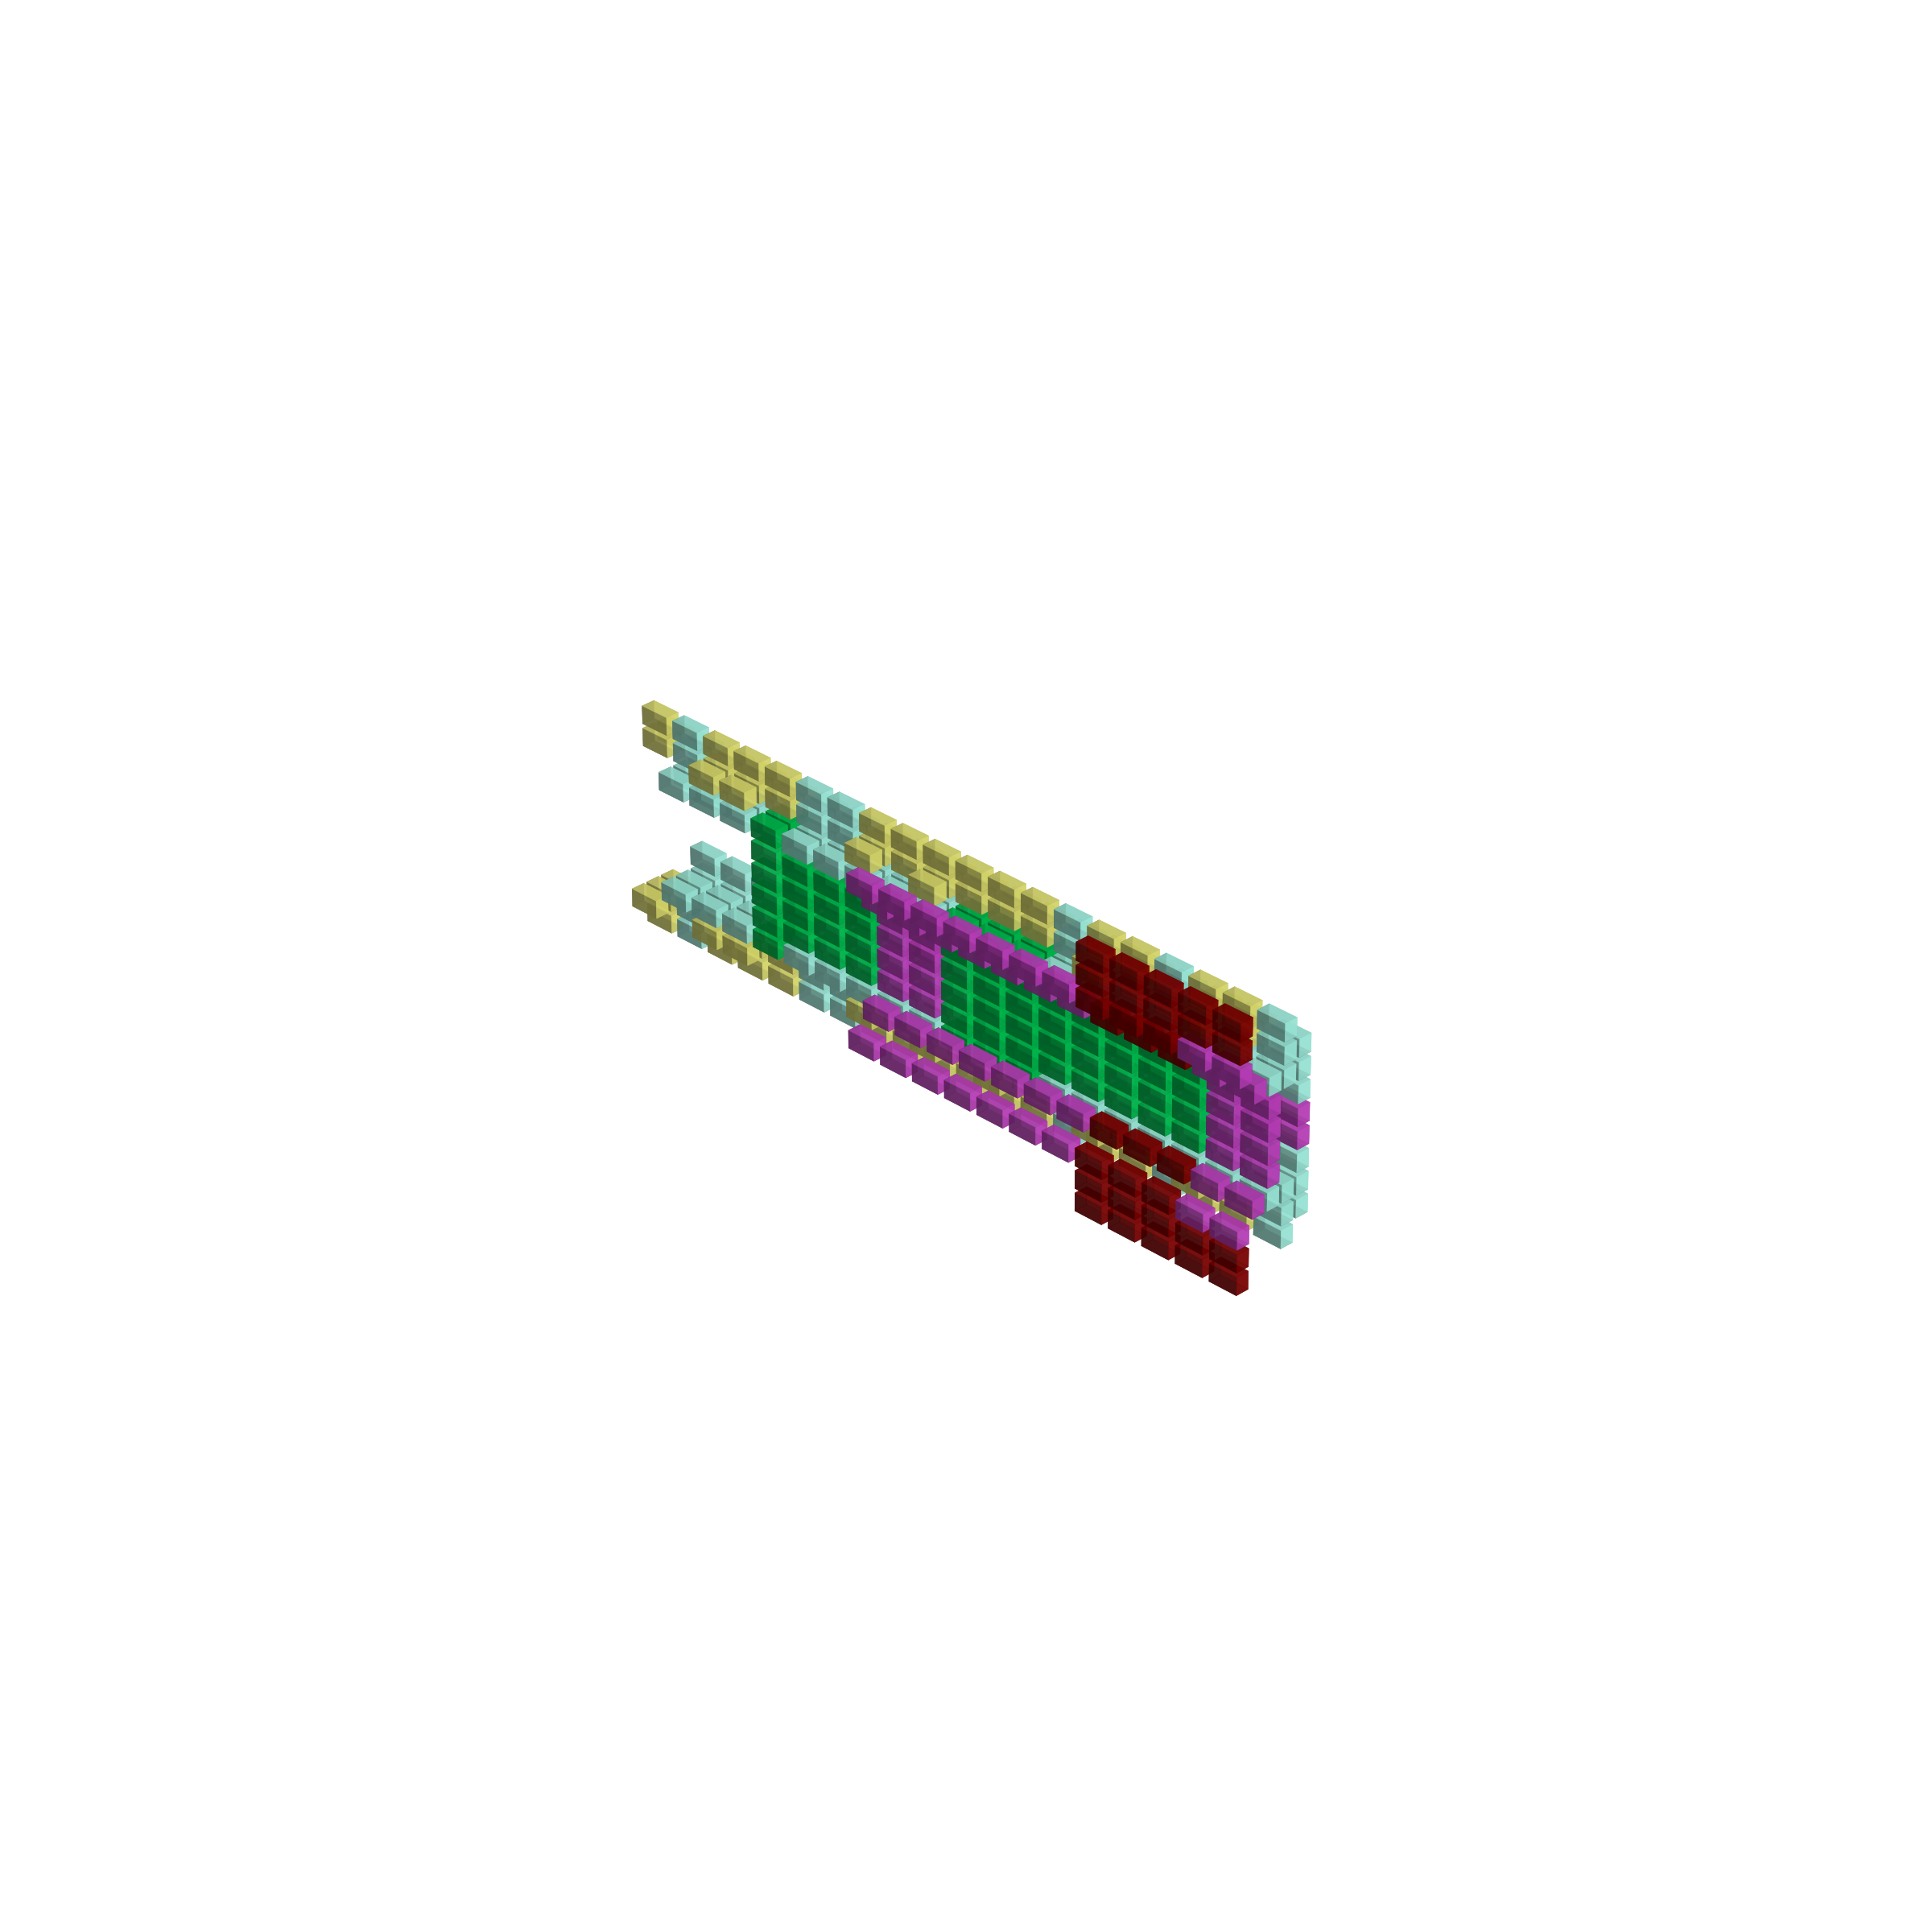
\includegraphics[width=8cm]{src/symmetries/pattern11_3-45.png}\\
        \vspace*{-8cm}
        \hspace*{2cm}
        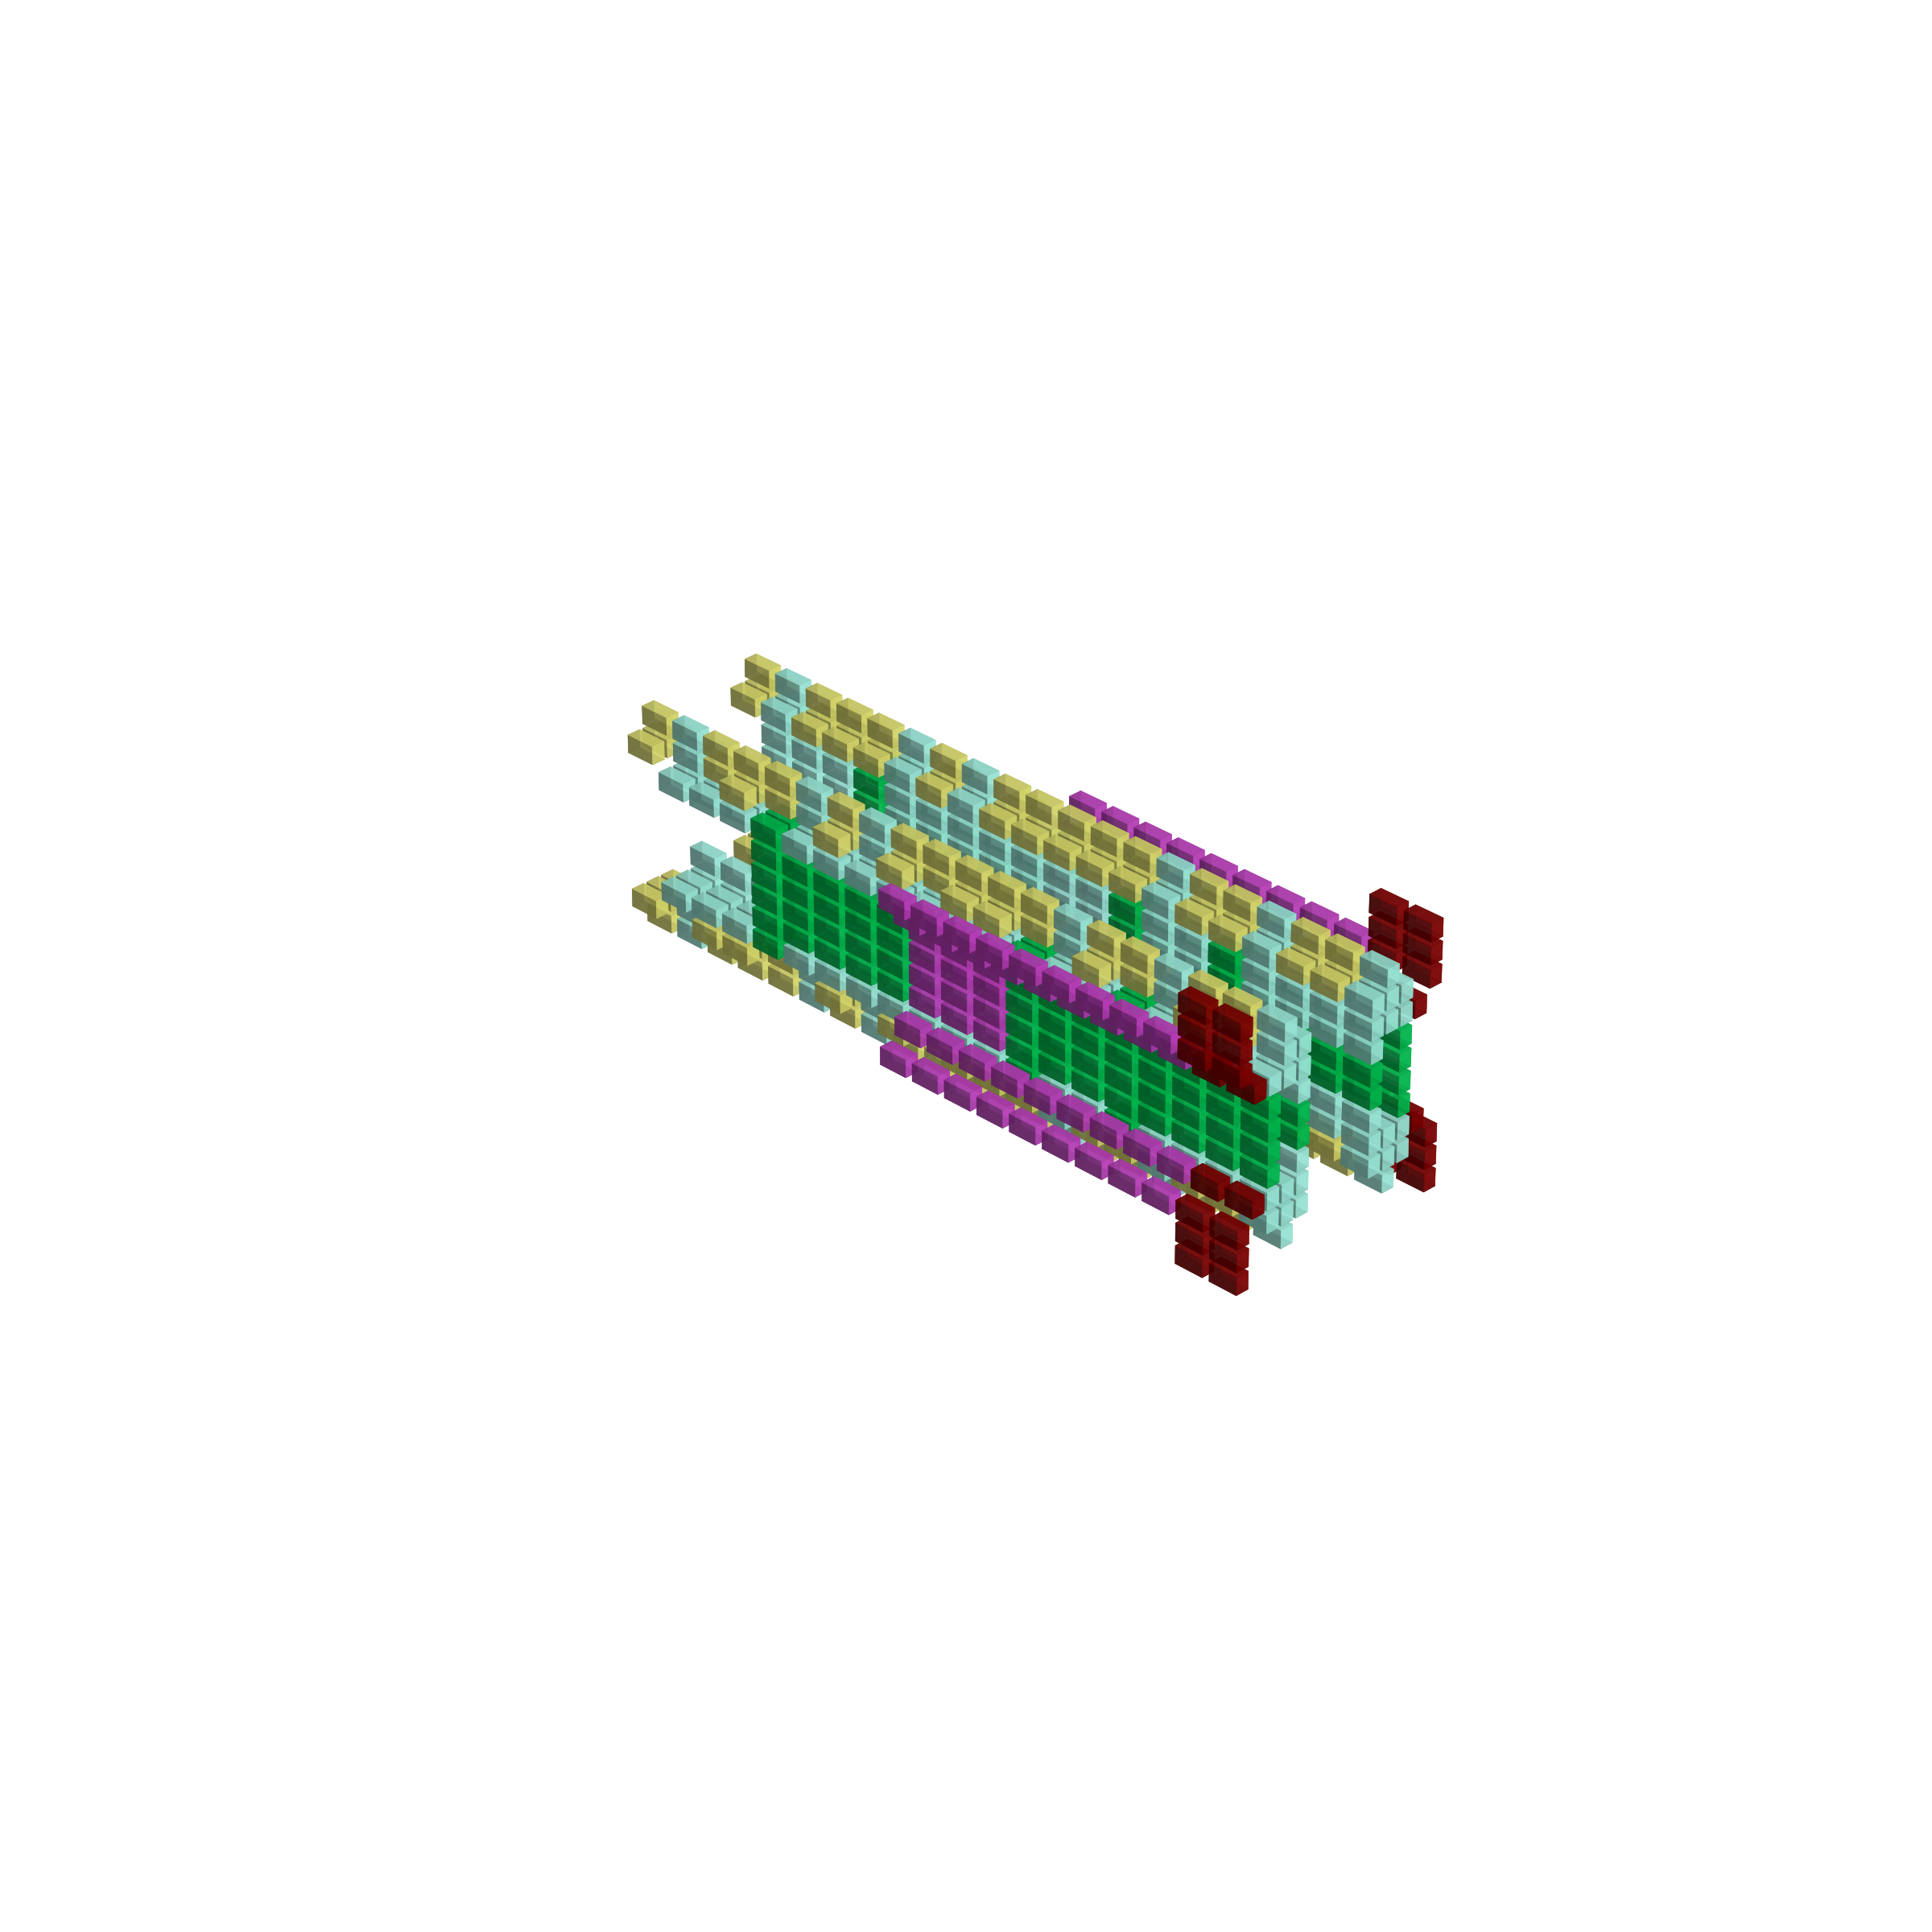
\includegraphics[width=8cm]{src/symmetries/pattern11_4-45.png}
        \vspace*{-2.5cm}
  \caption*{\getItem{11}}
  \end{figure}
\end{minipage}
\begin{minipage}[b]{0.50\linewidth}                                       
  \begin{figure}[H]
      \centering
        \vspace*{-1cm}
        \hspace*{-2cm}
        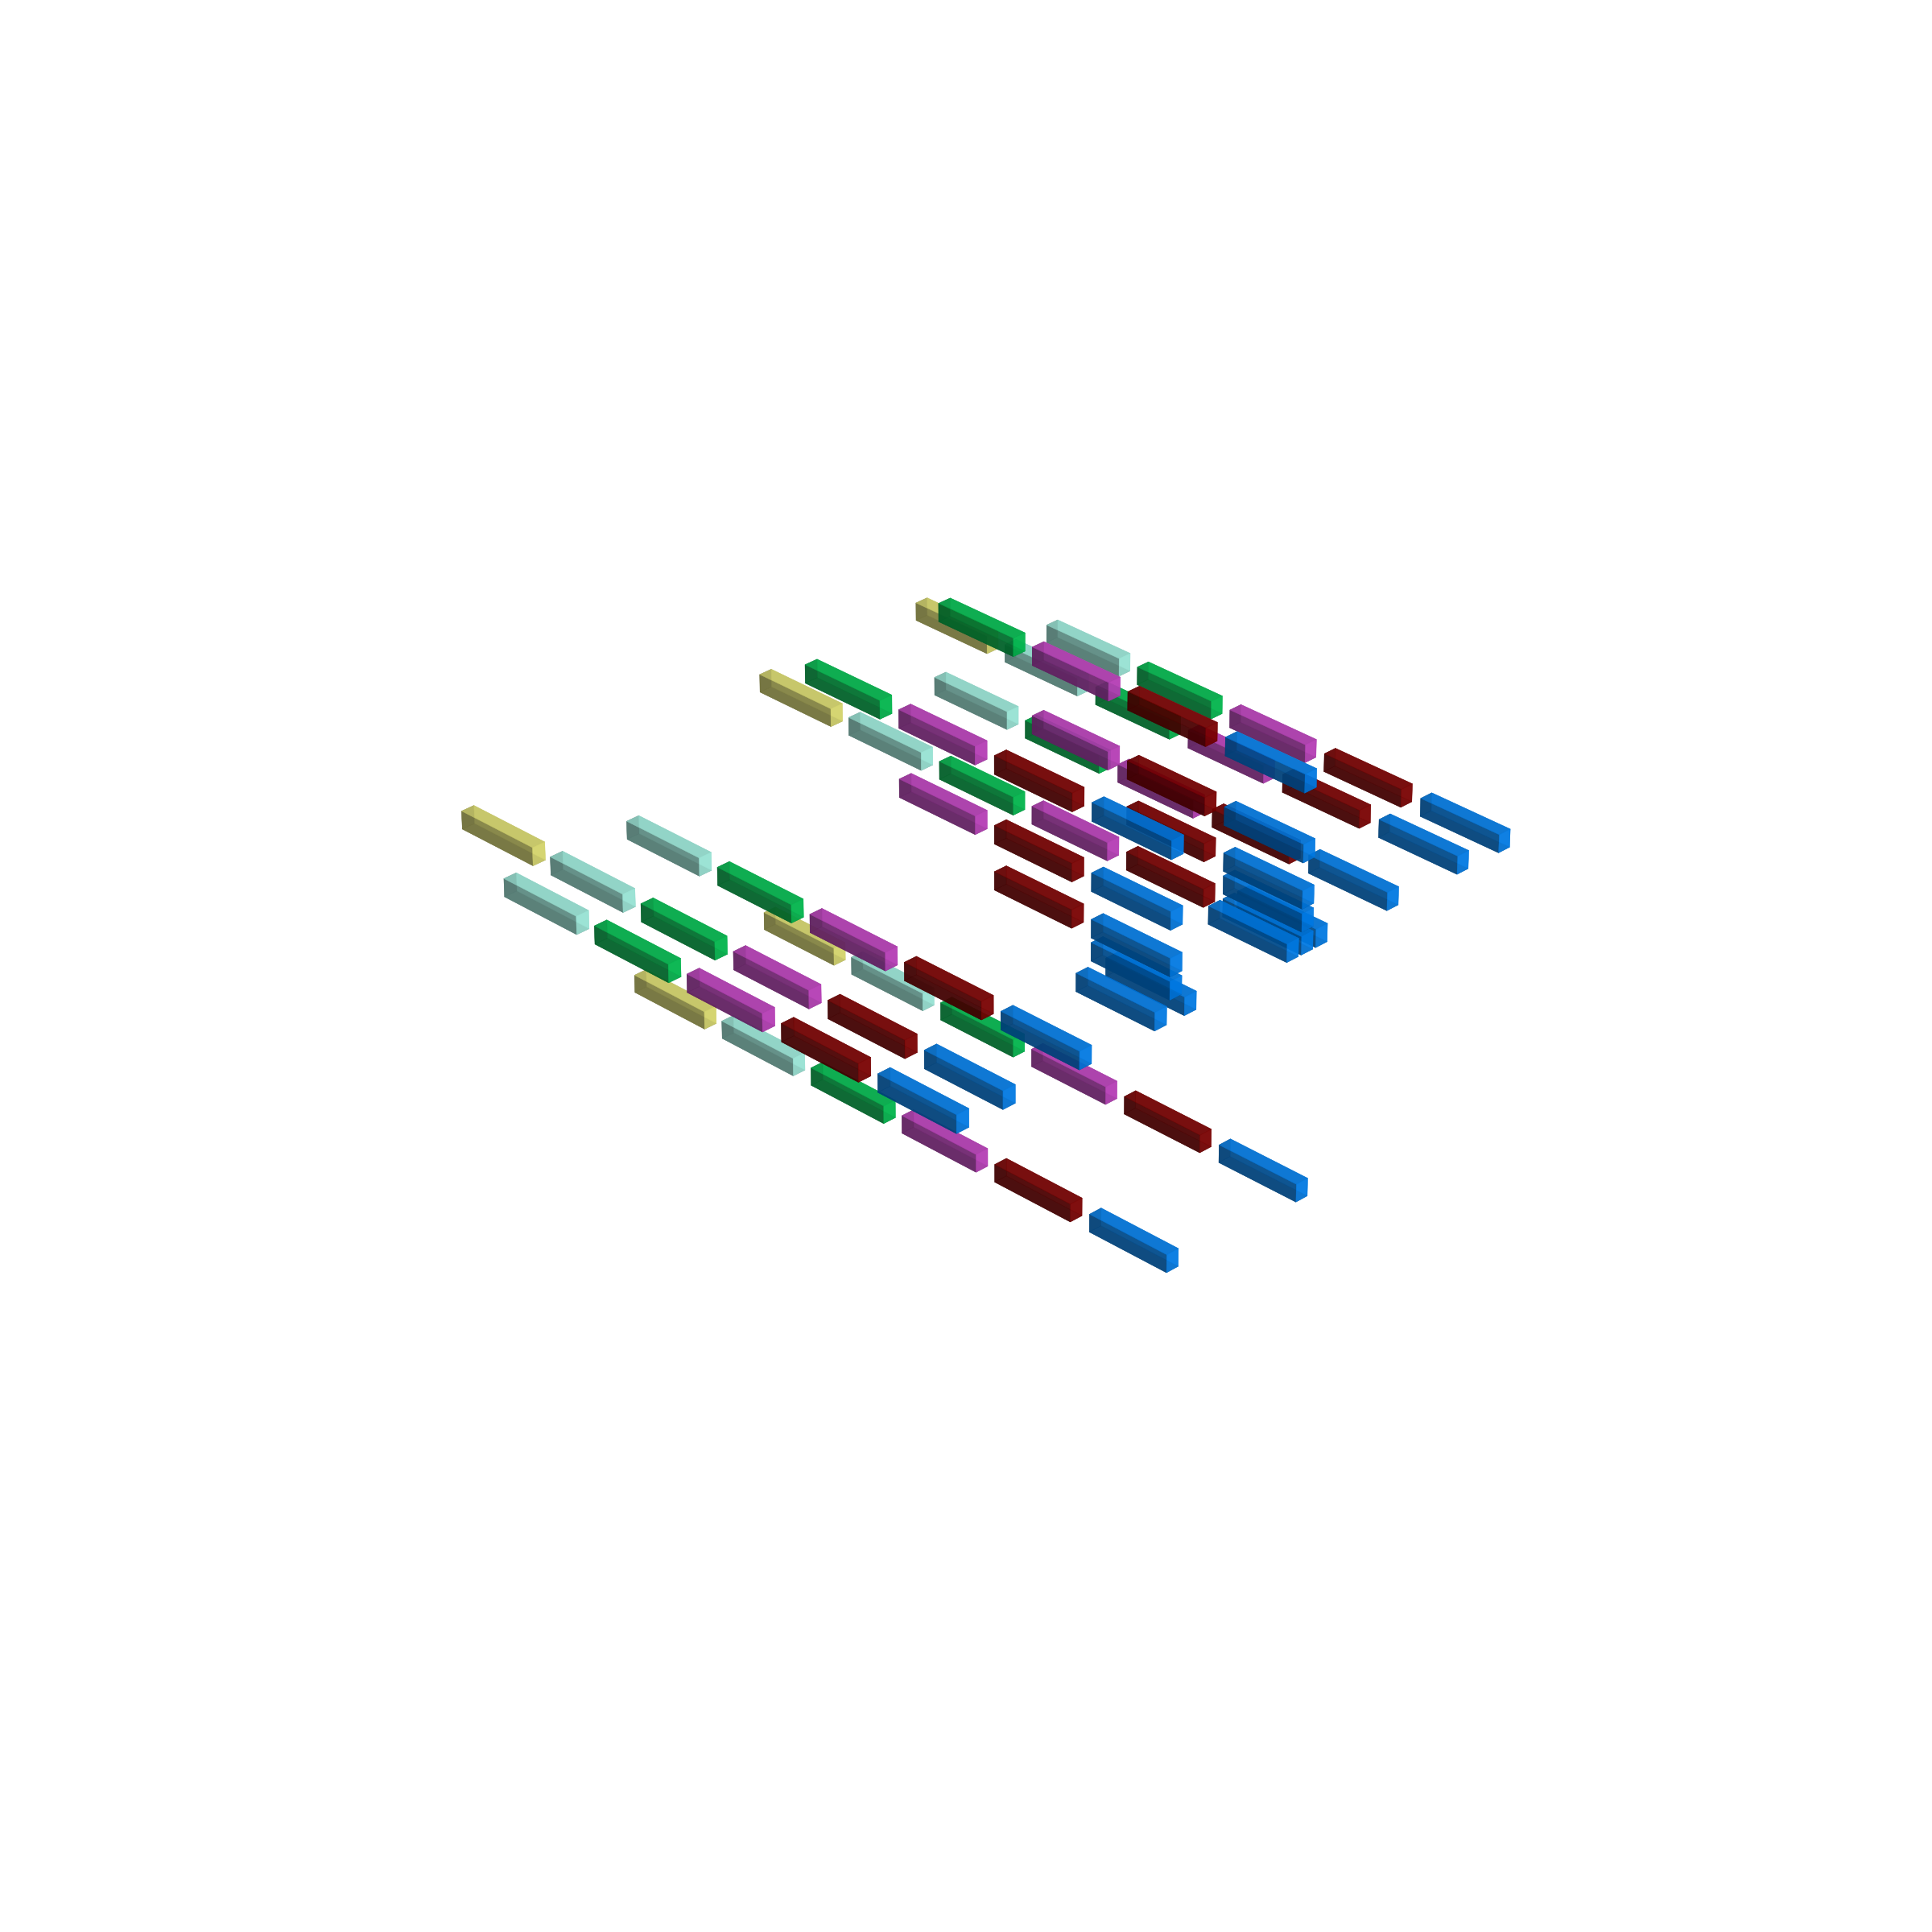
\includegraphics[width=8cm]{src/symmetries/pattern12_1-45.png}%
        \hspace*{-4cm}
        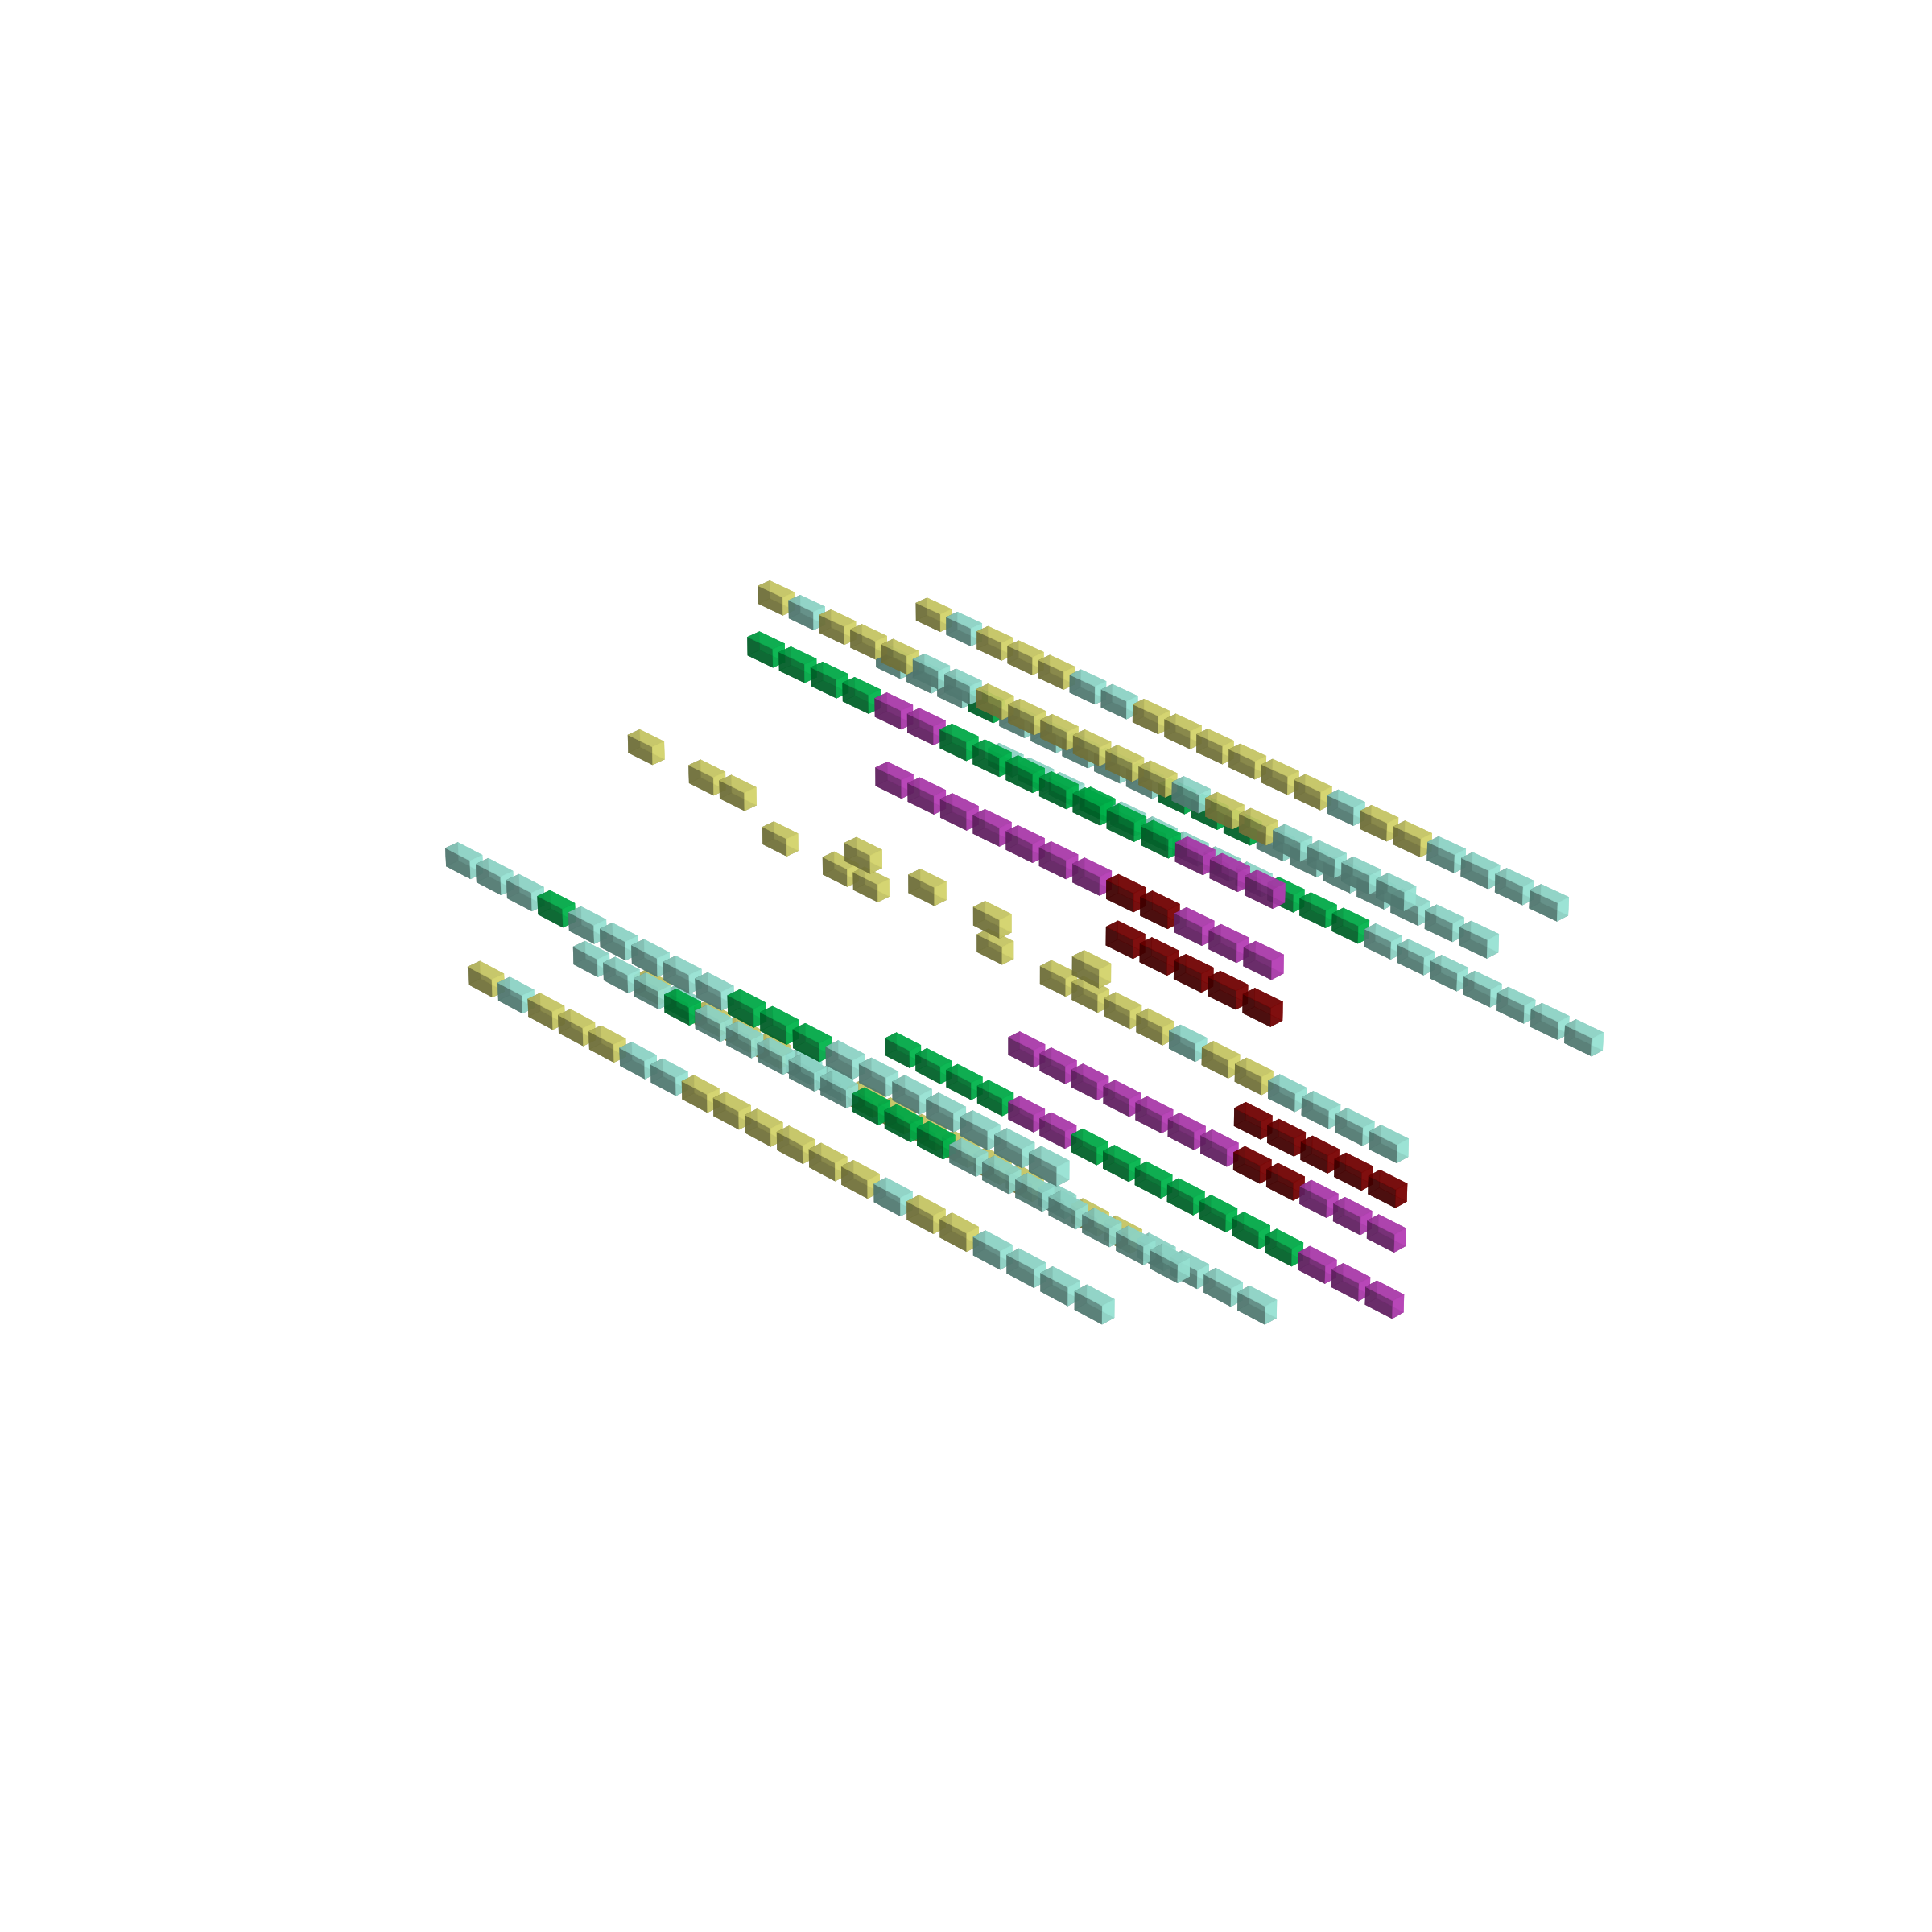
\includegraphics[width=8cm]{src/symmetries/pattern12_2-45.png}\\
        \vspace*{-5cm}
        \hspace*{-3cm}
        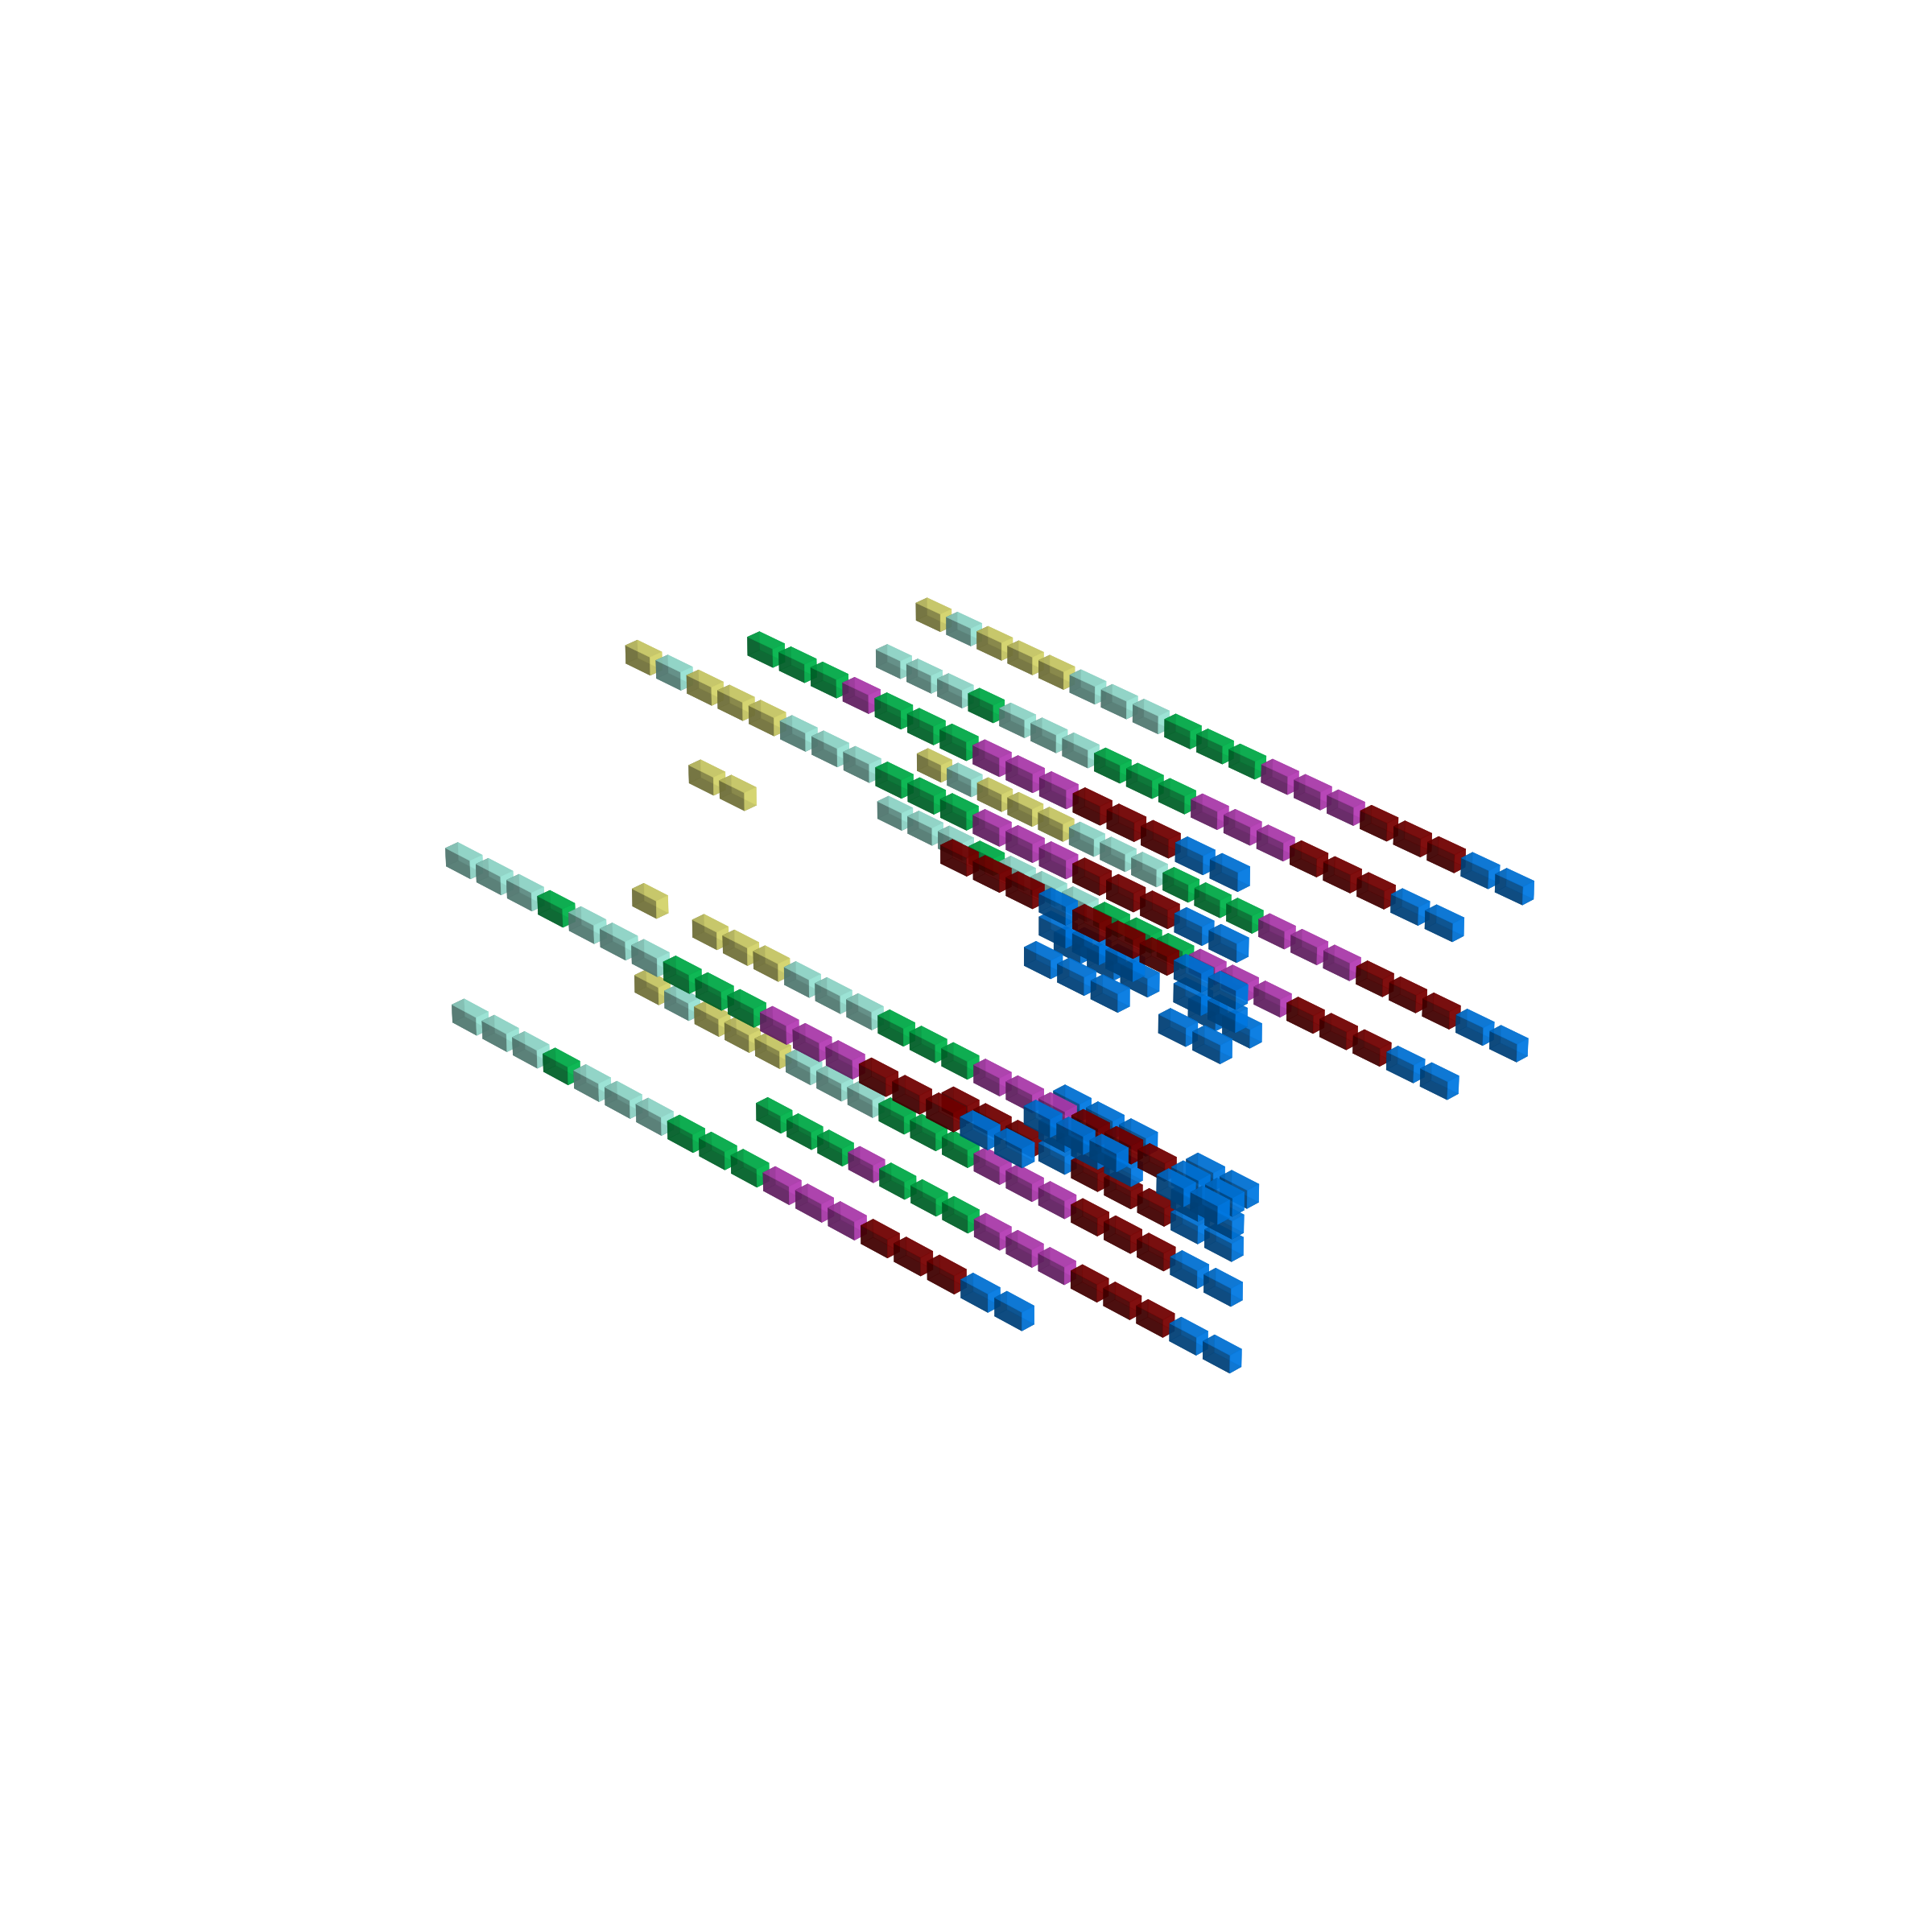
\includegraphics[width=8cm]{src/symmetries/pattern12_3-45.png}\\
        \vspace*{-8cm}
        \hspace*{2cm}
        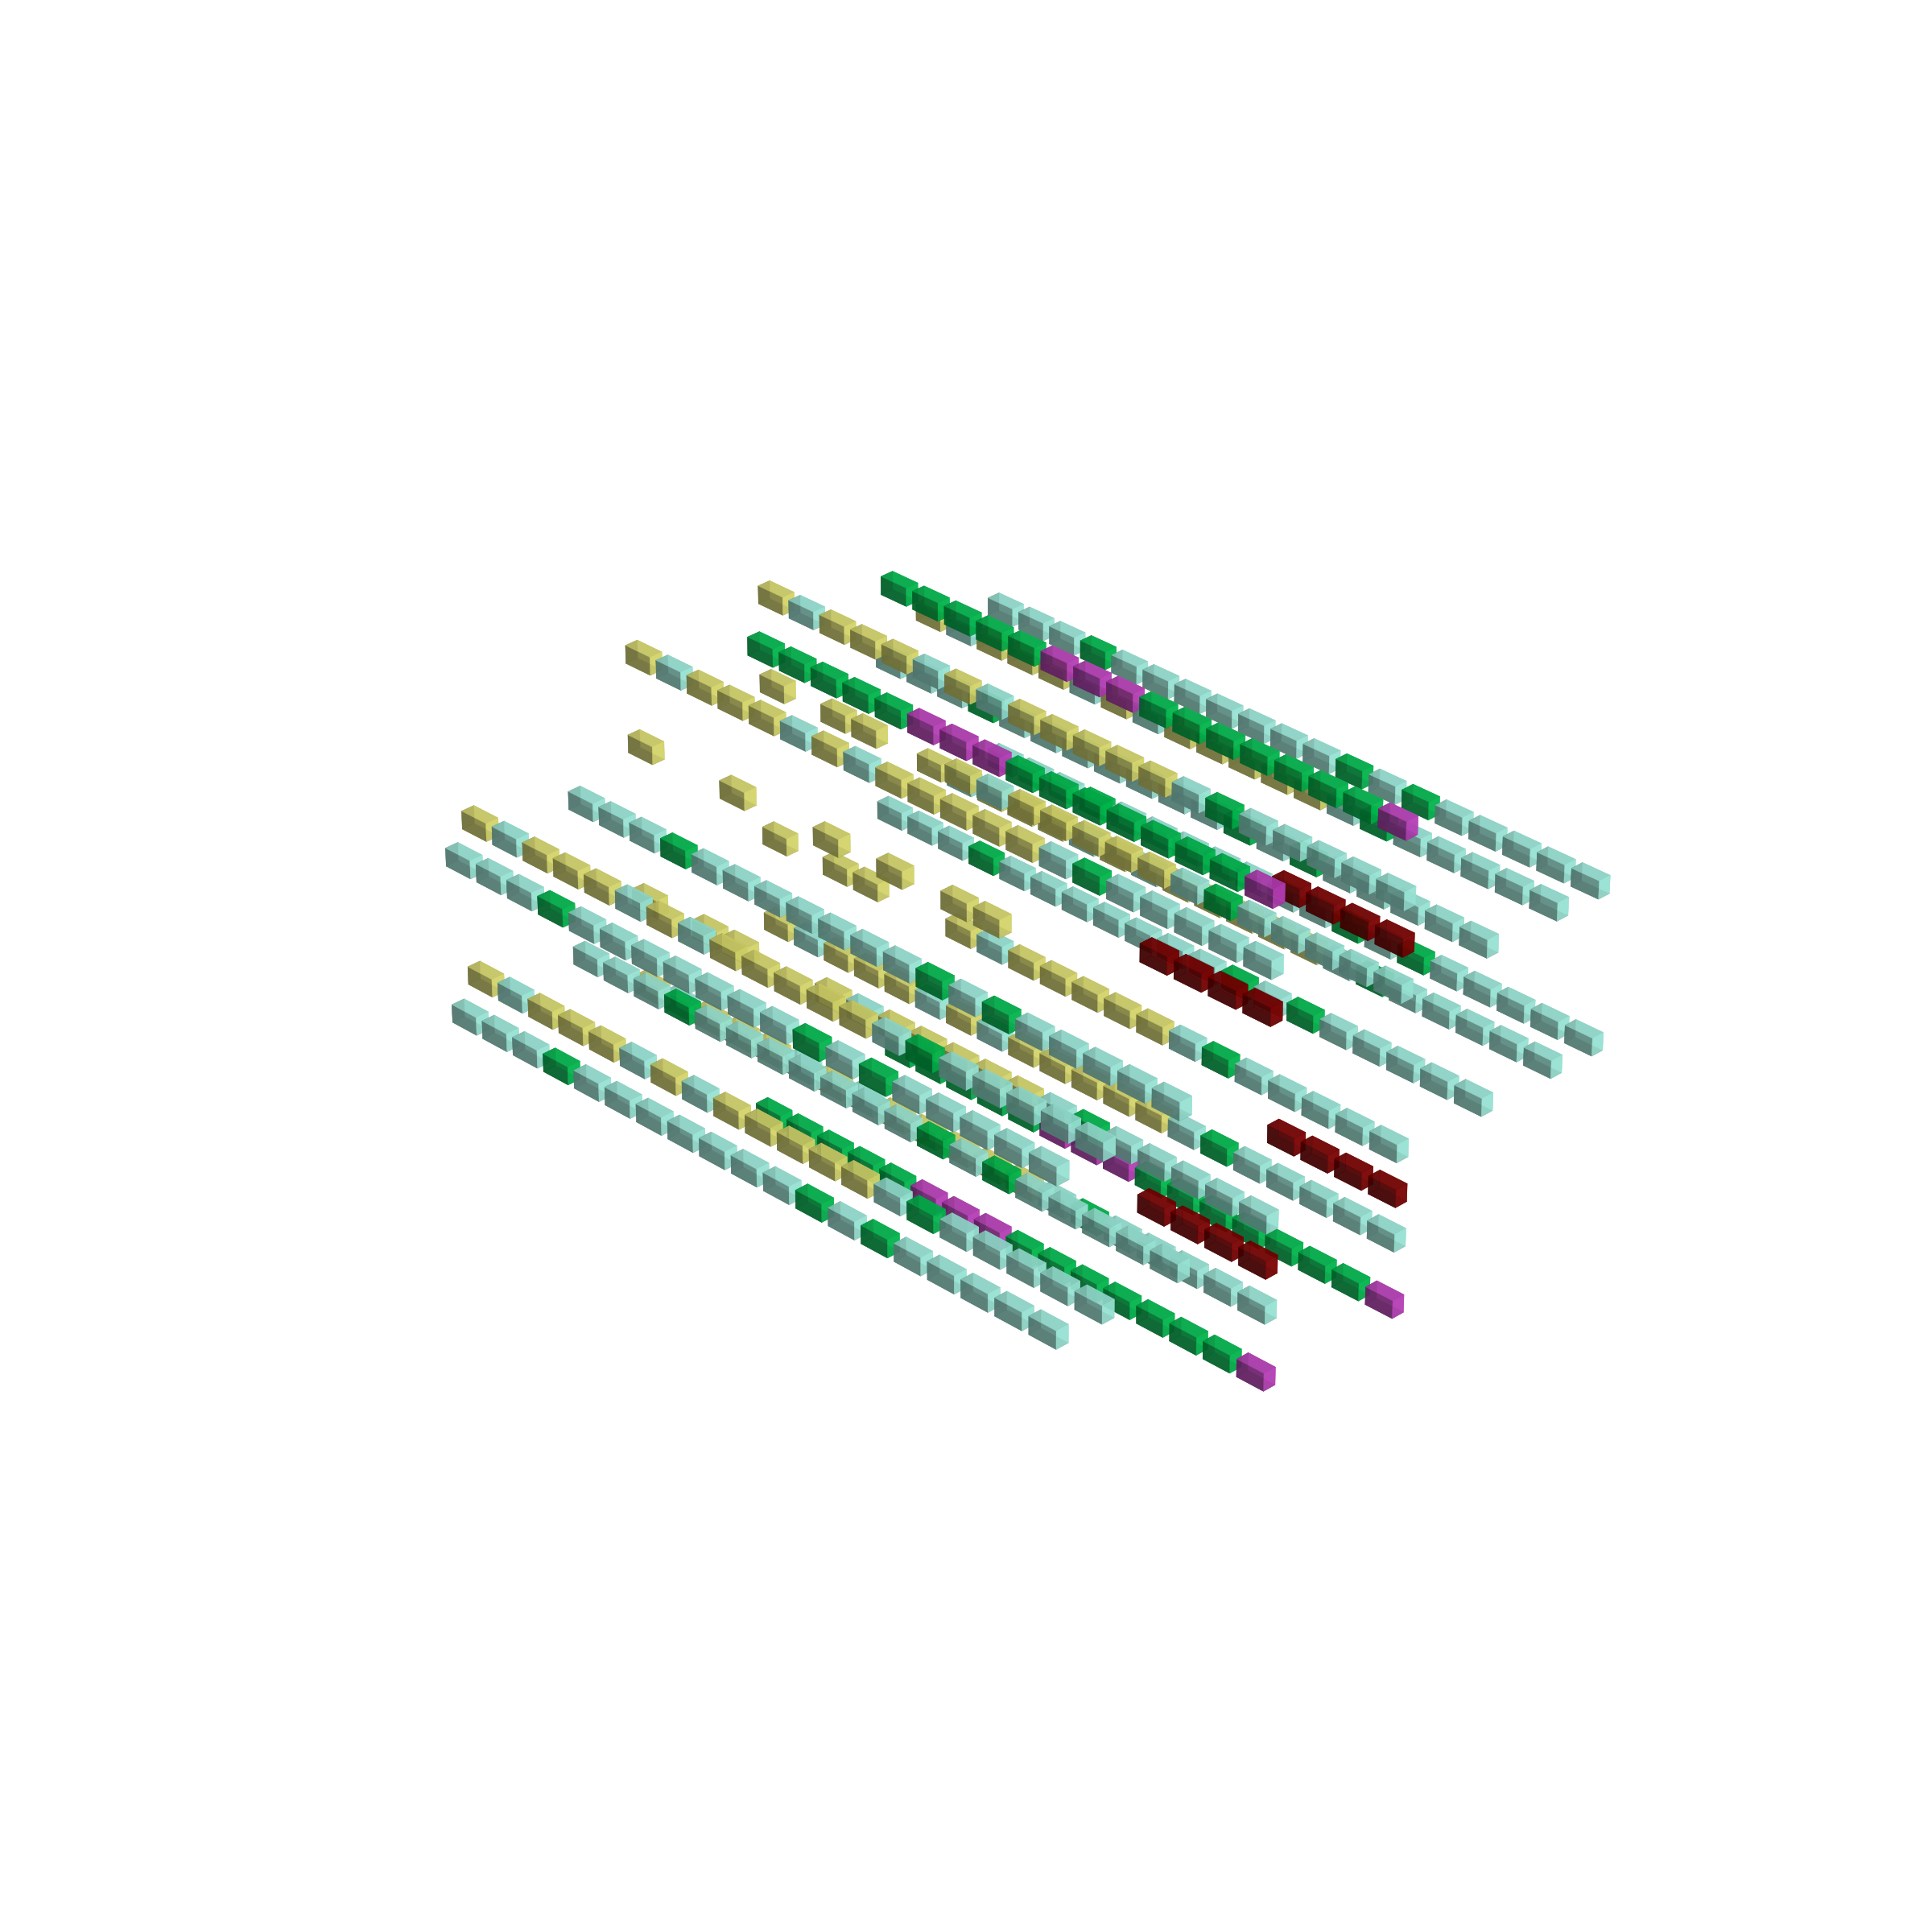
\includegraphics[width=8cm]{src/symmetries/pattern12_4-45.png}
        \vspace*{-2.5cm}
  \caption*{\getItem{12}}
  \end{figure}
\end{minipage}
\hspace{1cm}
\begin{minipage}[b]{0.50\linewidth}                                       
  \begin{figure}[H]
      \centering
        \vspace*{-1cm}
        \hspace*{-2cm}
        \includegraphics[width=8cm]{src/symmetries/pattern13_1-45.png}%
        \hspace*{-4cm}
        \includegraphics[width=8cm]{src/symmetries/pattern13_2-45.png}\\
        \vspace*{-5cm}
        \hspace*{-1cm}
        \includegraphics[width=8cm]{src/symmetries/pattern13_3-45.png}\\
        \vspace*{-8cm}
        \hspace*{2cm}
        \includegraphics[width=8cm]{src/symmetries/pattern13_4-45.png}
        \vspace*{-2.5cm}
  \caption*{\getItem{13}}
  \end{figure}
\end{minipage}

